\mag=1000
\documentclass[twoside]{report}
\usepackage{times}
\usepackage{amssymb}
\usepackage[dutch]{babel}
\usepackage{tikz}
\usepackage[psdextra]{hyperref}
\hypersetup{
    colorlinks=true,
    linkcolor=black,
    filecolor=magenta,      
    urlcolor=blue,
    pdftitle={Fysisch Formularium},
    }

\makeatletter

% tsemlines.sty: https://ctan.org/pkg/tsemlines

\def\newpic#1{%
   \def\emline##1##2##3##4##5##6{%
     \put(0,0){\tikz[remember picture,x=\unitlength,y=\unitlength,
       line width=\@wholewidth]{\draw(##1,##2)
         coordinate (em point #1 ##3) -- (##4,##5) coordinate
         (em point #1 ##6);
         \useasboundingbox (0,0) -- (em point #1
         ##3) -- (em point #1 ##6);}%
     }}}

\newpic{}

% changes to report.sty

\def\@makechapterhead#1{{\parindent 0pt\raggedright
\ifnum\c@secnumdepth >\m@ne\huge\bf\@chapapp{} \thechapter\par
\vskip 18pt\fi\Huge\bf #1\par
\nobreak\vskip 40pt}}

\def\@makeschapterhead#1{{\parindent 0pt\raggedright
\Huge\bf #1\par
\nobreak\vskip 40pt}}

% fancyheadings.sty

\def\lhead{\@ifnextchar[{\@xlhead}{\@ylhead}}
\def\@xlhead[#1]#2{\gdef\@elhead{#1}\gdef\@olhead{#2}}
\def\@ylhead#1{\gdef\@elhead{#1}\gdef\@olhead{#1}}

\def\chead{\@ifnextchar[{\@xchead}{\@ychead}}
\def\@xchead[#1]#2{\gdef\@echead{#1}\gdef\@ochead{#2}}
\def\@ychead#1{\gdef\@echead{#1}\gdef\@ochead{#1}}

\def\rhead{\@ifnextchar[{\@xrhead}{\@yrhead}}
\def\@xrhead[#1]#2{\gdef\@erhead{#1}\gdef\@orhead{#2}}
\def\@yrhead#1{\gdef\@erhead{#1}\gdef\@orhead{#1}}

\def\lfoot{\@ifnextchar[{\@xlfoot}{\@ylfoot}}
\def\@xlfoot[#1]#2{\gdef\@elfoot{#1}\gdef\@olfoot{#2}}
\def\@ylfoot#1{\gdef\@elfoot{#1}\gdef\@olfoot{#1}}

\def\cfoot{\@ifnextchar[{\@xcfoot}{\@ycfoot}}
\def\@xcfoot[#1]#2{\gdef\@ecfoot{#1}\gdef\@ocfoot{#2}}
\def\@ycfoot#1{\gdef\@ecfoot{#1}\gdef\@ocfoot{#1}}

\def\rfoot{\@ifnextchar[{\@xrfoot}{\@yrfoot}}
\def\@xrfoot[#1]#2{\gdef\@erfoot{#1}\gdef\@orfoot{#2}}
\def\@yrfoot#1{\gdef\@erfoot{#1}\gdef\@orfoot{#1}}

\newdimen\headrulewidth
\newdimen\footrulewidth
\newdimen\plainheadrulewidth
\newdimen\plainfootrulewidth
\newdimen\headwidth
\newif\if@fancyplain \@fancyplainfalse
\def\fancyplain#1#2{\if@fancyplain#1\else#2\fi}

\headrulewidth 0.5pt
\footrulewidth 0.5pt
\plainheadrulewidth\z@
\plainfootrulewidth\z@

\lhead[\fancyplain{}{\sl\rightmark}]{\fancyplain{}{\sl\leftmark}}
\rhead[\fancyplain{}{\sl\leftmark}]{\fancyplain{}{\sl\rightmark}}
\chead{}
\lfoot{}
\rfoot{}

\def\@fancyhead#1#2#3#4#5{#1\hbox to\headwidth{\vbox{\hbox
{\rlap{\parbox[b]{\headwidth}{\raggedright#2\strut}}\hfill
\parbox[b]{\headwidth}{\centering#3\strut}\hfill
\llap{\parbox[b]{\headwidth}{\raggedleft#4\strut}}}\headrule}}#5}

\def\@fancyfoot#1#2#3#4#5{#1\hbox to\headwidth{\vbox{\footrule
\hbox{\rlap{\parbox[t]{\headwidth}{\raggedright#2\strut}}\hfill
\parbox[t]{\headwidth}{\centering#3\strut}\hfill
\llap{\parbox[t]{\headwidth}{\raggedleft#4\strut}}}}}#5}

\def\headrule{{\if@fancyplain\headrulewidth\plainheadrulewidth\fi
\hrule\@height\headrulewidth\@width\headwidth \vskip-\headrulewidth}}

\def\footrule{{\if@fancyplain\footrulewidth\plainfootrulewidth\fi
\vskip-0.3\normalbaselineskip\vskip-\footrulewidth
\hrule\@width\headwidth\@height\footrulewidth\vskip0.3\normalbaselineskip}}

\def\ps@fancy{
\let\@mkboth\markboth
\@ifundefined{chapter}{\def\sectionmark##1{\markboth
{\uppercase{\ifnum \c@secnumdepth>\z@
\thesection\hskip 1em\relax \fi ##1}}{}}
\def\subsectionmark##1{\markright {\ifnum \c@secnumdepth >\@ne
\thesubsection\hskip 1em\relax \fi ##1}}}
{\def\chaptermark##1{\markboth {\uppercase{\ifnum \c@secnumdepth>\m@ne
\@chapapp\ \thechapter. \ \fi ##1}}{}}
\def\sectionmark##1{\markright{\uppercase{\ifnum \c@secnumdepth >\z@
\thesection. \ \fi ##1}}}}
\def\@oddhead{\@fancyhead\relax\@olhead\@ochead\@orhead\hss}
\def\@oddfoot{\@fancyfoot\relax\@olfoot\@ocfoot\@orfoot\hss}
\def\@evenhead{\@fancyhead\hss\@elhead\@echead\@erhead\relax}
\def\@evenfoot{\@fancyfoot\hss\@elfoot\@ecfoot\@erfoot\relax}
\headwidth\textwidth}
\def\ps@fancyplain{\ps@fancy \let\ps@plain\ps@plain@fancy}
\def\ps@plain@fancy{\@fancyplaintrue\ps@fancy}

% bezier.sty

\newcounter{@sc}
\newcounter{@scp}
\newcounter{@t}
\newlength{\@x}
\newlength{\@xa}
\newlength{\@xb}
\newlength{\@y}
\newlength{\@ya}
\newlength{\@yb}
\newsavebox{\@pt}
\def\bezier#1(#2,#3)(#4,#5)(#6,#7){\c@@sc#1\relax
\c@@scp\c@@sc\advance\c@@scp\@ne
\@xb #4\unitlength\advance\@xb -#2\unitlength\multiply\@xb\tw@
\@xa #6\unitlength\advance\@xa -#2\unitlength
\advance\@xa -\@xb\divide\@xa\c@@sc
\@yb #5\unitlength\advance\@yb -#3\unitlength\multiply\@yb\tw@
\@ya #7\unitlength\advance\@ya -#3\unitlength
\advance\@ya -\@yb\divide\@ya\c@@sc
\setbox\@pt\hbox{\vrule height\@halfwidth depth\@halfwidth
width\@wholewidth}\c@@t\z@
\put(#2,#3){\@whilenum{\c@@t<\c@@scp}\do
{\@x\c@@t\@xa\advance\@x\@xb\divide\@x\c@@sc\multiply\@x\c@@t
\@y\c@@t\@ya\advance\@y\@yb\divide\@y\c@@sc\multiply\@y\c@@t
\raise\@y\hbox to\z@{\hskip\@x\unhcopy\@pt\hss}\advance\c@@t\@ne}}}

\makeatother

\hoffset 0mm
\voffset 0mm
\parindent 0pt
\unitlength 1mm
\topmargin 0pt
\evensidemargin 0.385cm
\oddsidemargin 0.385cm
\marginparwidth 0.75in
\textwidth 15.4225cm
\textheight 53\baselineskip
\advance\textheight by \topskip
\advance\textheight by 5mm

\begin{document}

\typeout{Fysisch Formularium door ir. J.C.A. Wevers <johanw@xs4all.nl>}

\newfont{\sfd}{cmssdc10 scaled\magstep0}
\newfont{\cmu}{cmu10 scaled\magstep0}

\def\npar{\par\medskip}
%\def\vec#1{\mbox{\boldmath$#1$\unboldmath}}  % Uncomment this when you don't like the arrows
\def\rr{\vec{r}}
\def\vv{\vec{v}}
\def\aaa{\vec{a}}
\def\vvec#1{\vec{#1}\,}
\def\e#1{\vec{e}_{\rm #1}}
\def\ee#1{\vec{e}_{#1}}
\def\Q#1#2{\frac{\partial #1}{\partial #2}}
\def\QQ#1#2{\frac{\partial^2 #1}{\partial #2^2}}
\def\Qc#1#2#3{\left(\frac{\partial #1}{\partial #2}\right)_{#3}}
\def\LL{{\cal L}}
\def\RR{I\hspace{-1mm}R}
\def\NN{I\hspace{-1mm}N}
\def\TT{\mbox{\sfd T}}
\def\DD{\mbox{\sfd D}}
\def\half{\mbox{$\frac{1}{2}$}}
\def\kwart{\mbox{$\frac{1}{4}$}}
\def\av#1{\left\langle #1 \right\rangle}
\def\oiint{\int\hspace{-2ex}\int\hspace{-3ex}\bigcirc~}
\def\iint{\int\hspace{-1.5ex}\int}
\def\iiint{\int\hspace{-1.5ex}\int\hspace{-1.5ex}\int}
\def\dd{d\hspace{-1ex}\rule[1.25ex]{2mm}{0.4pt}}
\def\lrarrow{~\lower.2ex\hbox{$\rightarrow$}\kern-2.4ex\raise.7ex\hbox{$\leftarrow$}~}
\def\rlarrow{~\lower.2ex\hbox{$\leftarrow$}\kern-2.3ex\raise.7ex\hbox{$\rightarrow$}~}
\def\ne{n_{\rm e}}
\def\ni{n_{\rm i}}
\def\no{n_{\rm 0}}
\def\me{m_{\rm e}}
\def\mi{m_{\rm i}}
\def\Te{T_{\rm e}}
\def\Ti{T_{\rm i}}

% Labels in het tweede niveau Romeins nummeren.
\def\labelenumii{\Roman{enumii}.}
\def\theenumii{\Roman{enumii}}
\def\p@enumii{\theenumi}

\pagestyle{fancyplain}
\lhead[\fancyplain{}{\thepage}]{\fancyplain{}{\cmu Fysisch Formularium door ir. J.C.A. Wevers}}
\rhead[\fancyplain{}{\cmu Fysisch Formularium door ir. J.C.A. Wevers}]{\fancyplain{}{\thepage}}
\cfoot{\fancyplain{\thepage}{}}

\thispagestyle{empty}
\setcounter{page}{0}
\hrule
\rule{.4pt}{22.85cm}\hspace*{154mm}\rule{.4pt}{22.85cm}
\vspace*{-18cm}
\begin{center}
\Huge
\fbox{\fbox{Fysisch Formularium}}
\end{center}
\vspace{2cm}
\centerline{\Large\bf Door ir. J.C.A. Wevers}
\vspace{2cm}
\centerline{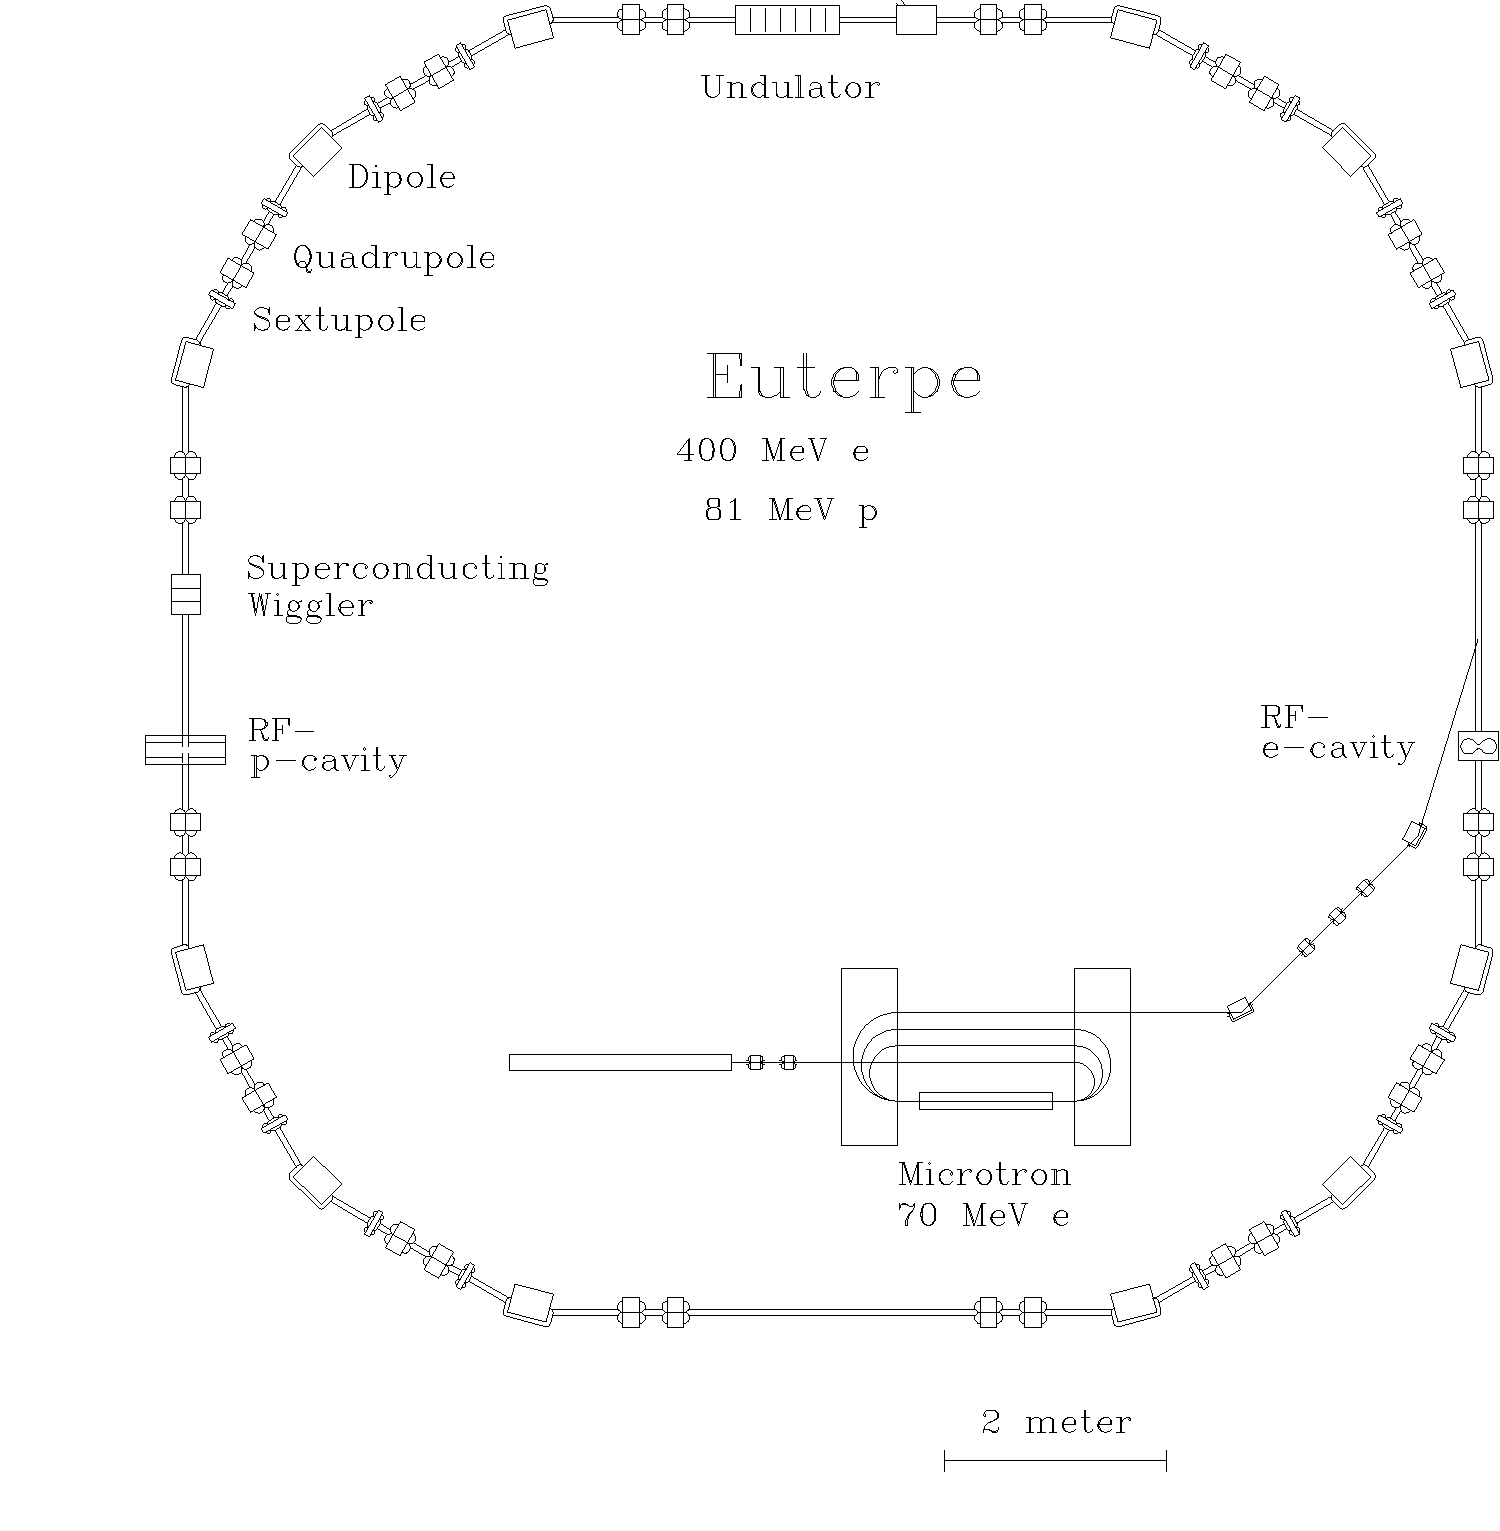
\includegraphics[width=10cm]{euterpe.pdf}~~~~~~}
\vfill
\hrule
\newpage
\thispagestyle{empty}
\copyright~1994, 2022~~J.C.A. Wevers\hfill Versie: 22 november 2022
\npar
\hrule
\par
\bigskip
Geachte lezer,
\npar
Dit document is een 108 pagina's tellend natuurkundig formuleboek op
universitair niveau. Het is bedoeld als naslagwerk voor iedereen die veel
formules op moet zoeken.
\npar
Dit document is, evenals een Engelstalige versie, te verkrijgen bij de
auteur, Johan Wevers\linebreak
(\href{mailto:johanw@xs4all.nl}{\tt johanw@xs4all.nl}).
\npar
Het is tevens te vinden op het WWW op \url{http://www.xs4all.nl/~johanw/index.html}.
Hier zijn tevens Postscript en PDF versies te vinden.
\npar
Het Fysisch Formularium werd gemaakt met behulp van MiK\TeX.
\npar
Indien U de layout waarin vectoren vet weergegeven worden prefereert kunt U
het commentaar voor het alternatieve {\tt $\backslash$vec} commando in de
\TeX\ file weghalen en hercompileren.
\npar
Ik houd me altijd aanbevolen voor opmerkingen en suggesties over het Fysisch
Formularium.
\npar
De Creative Commons Naamsvermelding 3.0 Nederland Licentie is van toepassing op dit werk.
Ga naar {\tt http://creativecommons.org/licenses/by/3.0/nl/} of stuur een brief naar Creative Commons,
171 Second Street, Suite 300, San Francisco, California, 94105, VS om deze licentie te bekijken.
\npar
Johan Wevers
\vfill
\hrule
\newpage

\pagenumbering{Roman}
\addcontentsline{toc}{chapter}{Inhoudsopgave}
\typeout{Inhoudsopgave}
\tableofcontents
\newpage

\pagenumbering{arabic}

\chapter*{\center Natuurconstanten}
\typeout{Natuurconstanten}
\addcontentsline{toc}{chapter}{Natuurconstanten}
\begin{center}
\begin{tabular}{||l|lll||}
\hline
{\bf Naam}&{\bf Symbool}&{\bf Waarde}&{\bf Eenheid}\\
\hline
\hline
Getal $\pi$                    &$\pi$&3,14159265358979323846...&\\
Getal e                        &e    &2,71828182845904523536...&\\
Constante van Euler&\multicolumn{3}{|l||}{$\gamma=\lim\limits_{n\rightarrow\infty}\left(\sum\limits_{k=1}^n 1/k-\ln(n)\right)=0,5772156649...$}\\
\hline
Elementaire lading             &$e$&$1,602176634\cdot10^{-19}$&C\rule{0pt}{13pt}\\
Gravitatieconstante            &$G,\kappa$&$6,67430(15)\cdot10^{-11}$&m$^3$kg$^{-1}$s$^{-2}$\\
Fijnstructuurconstante         &$\alpha=e^2/2hc\varepsilon_0$&$\approx1/137$&\\
Lichtsnelheid in vacu\"um      &$c$&$2,99792458\cdot10^8$&m/s (def)\\
Permittiviteit van het vacu\"um&$\varepsilon_0$&$8,8541878128(13)\cdot10^{-12}$&F/m\\
Permeabiliteit van het vacu\"um&$\mu_0$&$4\pi\cdot10^{-7}$&H/m\\
$(4\pi\varepsilon_0)^{-1}$     &&$8,9876\cdot10^9$&Nm$^2$C$^{-2}$\\
\hline
Constante van Planck           &$h$&$6,62607015\cdot10^{-34}$&Js\rule{0pt}{13pt}\\
Constante van Dirac            &$\hbar=h/2\pi$&$1,054571817\cdot10^{-34}$&Js\\
Bohrmagneton                   &$\mu_{\rm B}=e\hbar/2m_{\rm e}$&$9,2740100783(28)\cdot10^{-24}$&Am$^2$\\
Bohrstraal                     &$a_0$&$0,529177210903(80)$&\AA\\
Rydbergconstante               &$Ry$&13,605693122994(26)&eV\\
Comptongolflengte elektron     &$\lambda_{\rm Ce}=h/\me c$&$2,42631023867(73)\cdot10^{-12}$&m\\
Comptongolflengte proton       &$\lambda_{\rm Cp}=h/m_{\rm p}c$&$1,32140985539(40)\cdot10^{-15}$&m\\
Gereduceerde massa H-atoom     &$\mu_{\rm H}$&$9,1045755\cdot10^{-31}$&kg\\
\hline
Constante van Stefan-Boltzmann &$\sigma$&$5,670374419\cdot10^{-8}$&Wm$^{-2}$K$^{-4}$\rule{0pt}{13pt}\\
Constante van Wien             &$k_{\rm W}$&$2,897771955...\cdot10^{-3}$&mK\\
\hline
Gasconstante                   &$R$&8,31446261815324&J$\cdot$mol$^{-1}\cdot$K$^{-1}$\\
Getal van Avogadro             &$N_{\rm A}$&$6,02214076\cdot10^{23}$&mol$^{-1}$\\
Constante van Boltzmann        &$k=R/N_{\rm A}$&$1,380649\cdot10^{-23}$&J/K\\
\hline
Massa van het elektron         &$m_{\rm e}$&$9,1093837015(28)\cdot10^{-31}$&kg\rule{0pt}{13pt}\\
Massa van het proton           &$m_{\rm p}$&$1,67262192369(51)\cdot10^{-27}$&kg\\
Massa van het neutron          &$m_{\rm n}$&$1,67492749804(95)\cdot10^{-27}$&kg\\
Elementaire massaeenheid       &$m_{\rm u}=\frac{1}{12}m(^{12}_{~6}$C)&$1,66053906660(50)\cdot10^{-27}$&kg\\
Kernmagneton                   &$\mu_{\rm N}$&$5,050783699(31\cdot10^{-27}$&J/T\\
\hline
Diameter van de Zon            &$D_\odot$&$1392\cdot10^6$&m\rule{0pt}{13pt}\\
Massa van de Zon               &$M_\odot$&$1,989\cdot10^{30}$&kg\\
Rotatietijd van de Zon         &$T_\odot$&25,38&dag\\
Straal van de aarde            &$R_{\rm A}$&$6,378\cdot10^6$&m\\
Massa van de aarde             &$M_{\rm A}$&$5,976\cdot10^{24}$&kg\\
Rotatietijd van de aarde       &$T_{\rm A}$&23,96&uur\\
Omlooptijd aarde-zon           &Tropisch jaar&365,24219879&dag\\
Astronomische eenheid          &AE&$1,4959787066\cdot10^{11}$&m\\
Lichtjaar                      &lj&$9,4605\cdot10^{15}$&m\\
Parsec                         &pc&$3,0857\cdot10^{16}$&m\\
Constante van Hubble           &$H$&$\approx(75\pm25)$&km$\cdot$s$^{-1}\cdot$Mpc$^{-1}$\\
\hline
\end{tabular}
\end{center}

\renewcommand{\chaptermark}[1]{\markboth{#1}{#1}}
\lhead[\fancyplain{}{\thepage}]{\fancyplain{}{\cmu Hoofdstuk \thechapter: \leftmark}}
\rhead[\fancyplain{}{\cmu Fysisch Formularium door ir. J.C.A. Wevers}]{\fancyplain{}{\thepage}}

\chapter{Mechanica}
\typeout{Mechanica}
\section{Puntkinematica in een vast stelsel}
\subsection{Definities}
De plaats $\rr$, de snelheid $\vv$ en de versnelling $\aaa$ zijn gedefinieerd
als:
$\rr=(x,y,z)$, $\vv=(\dot{x},\dot{y},\dot{z})$, $\aaa=(\ddot{x},\ddot{y},\ddot{z})$.
Er geldt:
\[
s(t)=s_0+\int|\vv(t)|dt~;~~~\rr(t)=\rr_0+\int\vv(t)dt~;~~~\vv(t)=\vv_0+\int\aaa(t)dt
\]
Bij constante versnelling geldt dus: $v(t)=v_0+at$ en $s(t)=s_0+v_0t+\half at^2$.
\npar
Voor de eenheidsrichtingsvectoren $\perp$ op de baan $\e{t}$ en evenwijdig
daaraan $\e{n}$ geldt:
\[
\e{t}=\frac{\vv}{|\vv|}=\frac{d\rr}{ds}~~~\dot{\e{t}}=
\frac{v}{\rho}\e{n}~;~~~\e{n}=\frac{\dot{\e{t}}}{|\dot{\e{t}}|}
\]
Voor de {\it kromming} $k$ en de {\it kromtestraal} $\rho$ geldt:
\[
\vec{k}=\frac{d\e{t}}{ds}=\frac{d^2\rr}{ds^2}=\left|\frac{d\varphi}{ds}\right|
~;~~~\rho=\frac{1}{|k|}
\]
\subsection{Poolco\"ordinaten}
Poolco\"ordinaten worden gegeven door: $x=r\cos(\theta)$, $y=r\sin(\theta)$.
Hieruit volgt voor de eenheidsvectoren: $\dot{\ee{r}}=\dot{\theta}\ee{\theta}$,
$\dot{\ee{\theta}}=-\dot{\theta}\ee{r}$
\npar
De snelheid en versnelling volgen uit: $\rr=r\ee{r}$,
$\vv=\dot{r}\ee{r}+r\dot{\theta}\ee{\theta}$,
$\aaa=(\ddot{r}-r\dot{\theta}^2)\ee{r}+(2\dot{r}\dot{\theta}+r\ddot{\theta})\ee{\theta}$.

\section{Relatieve beweging}
Voor de beweging van een punt D t.o.v. een punt Q geldt:
$\displaystyle\rr_{\rm D}=\rr_{\rm Q}+\frac{\vec{\omega}\times\vv_{\rm Q}}{\omega^2}$,
met $\vec{\rm QD}=\rr_{\rm D}-\rr_{\rm Q}$ en $\omega=\dot{\theta}$.
\npar
Verder geldt:
$\alpha=\ddot{\theta}$. Het accent $'$ betekent: de betreffende grootheid geldt
in het bewegende co\"ordinatenstelsel. In een bewegend stelsel geldt:\\
$\vv=\vv_{\rm Q}+\vv\,'+\vec{\omega}\times\rr\,'$ en
$\aaa=\aaa_{\rm Q}+\aaa\,'+\vec{\alpha}\times\rr\,'+2\vec{\omega}\times\vv\,'+\vec{\omega}\times(\vec{\omega}\times\rr\,')$\\
met $\vec{\omega}\times(\vec{\omega}\times\rr\,')=-\omega^2\rr\,'_n$

\section{Puntdynamica in een vast stelsel}
\subsection{Kracht, impuls(moment), energie}
De 2e wet van Newton geeft het verband tussen een kracht op een voorwerp en
de resulterende versnelling daarvan, waarin de {\it impuls} gegeven is door:
$\vec{p}=m\vv$:
\[
\vec{F}(\rr,\vv,t)=\frac{d\vec{p}}{dt}=\frac{d(m\vv\,)}{dt}=m\frac{d\vv}{dt}+
\vv\,\frac{dm}{dt}\mathop{=}\limits^{m={\rm const}}m\aaa
\]
De 3e wet van Newton luidt: $\vec{F}_{\rm actie}=-\vec{F}_{\rm reactie}$.
\npar
Voor het vermogen $P$ geldt: $P=\dot{W}=\vec{F}\cdot\vv$. Voor de totale
energie $W$, de kinetische energie $T$ en de potenti\"ele energie $U$ geldt:
$W=T+U~;~~~\dot{T}=-\dot{U}$ met $T=\half mv^2$.
\npar
De {\it stoot} $\vec{S}$ is gegeven door:
$\displaystyle\vec{S}=\Delta\vec{p}=\int\vec{F}dt$
\npar
De door een kracht geleverde arbeid $A$ is
$\displaystyle A=\int\limits_1^2\vec{F}\cdot d\vec{s}=\int\limits_1^2F\cos(\alpha)ds$
\npar
Het krachtmoment $\vec{\tau}$ hangt samen met het impulsmoment $\vec{L}$:~~
$\vec{\tau}=\dot{\vec{L}}=\rr\times\vec{F}$; en\\
$\vec{L}=\rr\times\vec{p}=m\vv\times\rr$, $|\vvec{L}|=mr^2\omega$. Er geldt
\[
\tau=-\Q{U}{\theta}
\]
Voorwaarden voor een mechanisch evenwicht zijn dus: $\sum\vec{F}_i=0$ en
$\sum\vec{\tau}_i=0$.
\npar
De {\it wrijvingskracht} is meestal evenredig met de normaalkracht, behalve
bij het op gang komen van de beweging, wanneer er een drempel overwonnen
moet worden: $F_{\rm wrijv}=f\cdot F_{\rm norm}\cdot\e{t}$.

\subsection{Conservatief krachtveld}
Een conservatieve kracht is te schrijven als de gradi\"ent van een potentiaal:
$\vec{F}_{\rm cons}=-\vec{\nabla}U$. Hieruit volgt dat
$\nabla\times\vec{F}=\vec{0}$. Voor zo'n krachtveld geldt tevens:
\[
\oint\vec{F}\cdot d\vec{s}=0~\Rightarrow~U=U_0-\int\limits_{r_0}^{r_1}\vec{F}\cdot d\vec{s}
\]
De arbeid die een conservatief veld verricht hangt dus niet af van de
gevolgde baan, maar slechts van het begin- en eindpunt van de beweging.

\subsection{Gravitatie}
De Newtonse gravitatiewet luidt (in de ART schrijft men ook $\kappa$ i.p.v. $G$):
\[
\vec{F}_{\rm g}=-G\frac{m_1 m_2}{r^2}\ee{r}
\]
Hieruit volgt voor de gravitatiepotentiaal $V=-Gm/r$. Uit Gauss volgt dan:
$\nabla^2 V=4\pi G\varrho$.

\subsection{Baanvergelijkingen}
Als $V=V(r)$ volgt uit de Lagrangevergelijking voor $\phi$ behoud van
impulsmoment:
\[
\Q{\LL}{\phi}=\Q{V}{\phi}=0\Rightarrow\frac{d}{dt}(mr^2\phi)=0\Rightarrow L_z=mr^2\phi=\mbox{constant}
\]
Voor de straal als functie van de tijd is dan af te leiden dat:
\[
\left(\frac{dr}{dt}\right)^2=\frac{2(W-V)}{m}-\frac{L^2}{m^2r^2}
\]
De hoekvergelijking luidt nu:
\[
\phi-\phi_0=\int\limits_0^r\left[\frac{mr^2}{L}\sqrt{\frac{2(W-V)}{m}-\frac{L^2}{m^2r^2}}~\right]^{-1}dr
\stackrel{r^{-2}{\rm veld}}{=}
\arccos\left(1+\frac{\frac{1}{r}-\frac{1}{r_0}}{\frac{1}{r_0}+km/L_z^2}\right)
\]
als $F=F(r)$: $L=$constant, als $F$ conservatief is, geldt $W=$constant, als
$\vec{F}\perp\vv$ dan is $\Delta T=0$ en $U=0$.

\subsubsection{De baanvergelijkingen van Kepler}
In een krachtveld $F=kr^{-2}$ veld zijn banen kegelsneden met het
krachtcentrum in een brandpunt (1e wet van Kepler). De baanvergelijking luidt:
\[
r(\theta)=\frac{\ell}{1+\varepsilon\cos(\theta-\theta_0)}~,~~\mbox{ofwel:~~}
x^2+y^2=(\ell-\varepsilon x)^2
\]
met
\[
\ell=\frac{L^2}{G\mu^2M_{\rm tot}}~;~~~\varepsilon^2=1+\frac{2WL^2}{G^2\mu^3M^2_{\rm tot}}=1-\frac{\ell}{a}
~;~~~a=\frac{\ell}{1-\varepsilon^2}=\frac{k}{2W}
\]
$a$ is de lengte van de halve lange as van de ellipsbaan in het geval de baan
gesloten is. De halve korte as $b=\sqrt{a\ell}$. $\varepsilon$ is de
{\it excentriciteit} van de baan. Banen met gelijke $\varepsilon$ zijn
gelijkvormig. Er zijn nu 5 soorten banen mogelijk:
\begin{enumerate}
\item $k<0$ en $\varepsilon=0$: een cirkel.
\item $k<0$ en $0<\varepsilon<1$: een ellips.
\item $k<0$ en $\varepsilon=1$: een parabool.
\item $k<0$ en $\varepsilon>1$: een hyperbool naar het krachtcentrum toe gekromd.
\item $k>0$ en $\varepsilon>1$: een hyperbool van het krachtcentrum af gekromd.
\end{enumerate}
Andere combinaties zijn niet mogelijk: in een afstotend veld is de totale
energie positief dus $\varepsilon>1$.
\npar
Indien $A(t_1,t_2)$ het oppervlak is tussen de baan die doorlopen is tussen
$t_1$ en $t_2$ en het brandpunt C waaromheen de planeet draait luidt de 2e
wet van Kepler (de perkenwet):
\[
A(t_1,t_2)=\frac{L_{\rm C}}{2m}(t_2-t_1)
\]
De 3e wet van Kepler luidt, met $T$ de omlooptijd en $M_{\rm tot}$ de totale
massa van het systeem:
\[
\frac{T^2}{a^3}=\frac{4\pi^2}{GM_{\rm tot}}
\]
\subsection{De viriaalstelling}
De viriaalstelling voor 1 deeltje luidt:
\[
\av{m\vv\cdot\rr}=0\Rightarrow\av{T}=-\half\av{\vec{F}\cdot\rr}=\half\av{r\frac{dU}{dr}}=
\half n\av{U}\mbox{ als } U=-\frac{k}{r^n}
\]
De viriaalstelling voor een verzameling deeltjes luidt:
\[
\av{T}=-\half\av{\sum\limits_{\rm deeltjes}\vec{F}_i\cdot\rr_i+
\sum\limits_{\rm paren}\vec{F}_{ij}\cdot\rr_{ij}}
\]
Deze stellingen zijn ook te schrijven als $2E_{\rm kin}+E_{\rm pot}=0$.

\section{Puntdynamica in een bewegend stelsel}
\subsection{Schijnkrachten}
De totale kracht in een bewegend co\"ordinatenstelsel wordt gevonden door de
schijnkrachten af te trekken van de krachten die in het referentiestelsel
werken: $\vec{F}\,'=\vec{F}-\vec{F}_{\rm schijn}$. De verschillende
schijnkrachten worden gegeven door:
\begin{enumerate}
\item Oorsprongstransformatie: $F_{\rm oor}=-m\aaa_a$
\item Rotatie: $\vec{F}_{\alpha}=-m\vec{\alpha}\times\rr\,'$
\item Corioliskracht: $F_{\rm cor}=-2m\vec{\omega}\times\vv$
\item Centrifugale kracht: $\vec{F}_{\rm cf}=m\omega^2\rr_n\,'=-\vec{F}_{\rm cp}$
      ;~~$\displaystyle\vec{F}_{\rm cp}=-\frac{mv^2}{r}\ee{r}$
\end{enumerate}

\subsection{Tensorvorm}
Transformatie van de Newtonse bewegingsvergelijkingen naar $x^\alpha=x^\alpha(x)$:
\[
\frac{dx^\alpha}{dt}=\Q{x^\alpha}{\bar{x}^\beta}\frac{d\bar{x}^\beta}{dt};
\]
Uit de kettingregel volgt:
\[
\frac{d}{dt}\frac{dx^\alpha}{dt}=\frac{d^2x^\alpha}{dt^2}=\frac{d}{dt}
\left(\Q{x^\alpha}{\bar{x}^\beta}\frac{d\bar{x}^\beta}{dt}\right)=
\Q{x^\alpha}{\bar{x}^\beta}\frac{d^2\bar{x}^\beta}{dt^2}+
\frac{d\bar{x}^\beta}{dt}\frac{d}{dt}\left(\Q{x^\alpha}{\bar{x}^\beta}\right)
\]
dus:
\[
\frac{d}{dt}\Q{x^\alpha}{\bar{x}^\beta}=\Q{}{\bar{x}^\gamma}\Q{x^\alpha}{\bar{x}^\beta}\frac{d\bar{x}^\gamma}{dt}=
\frac{\partial^2x^\alpha}{\partial\bar{x}^\beta\partial\bar{x}^\gamma}\frac{d\bar{x}^\gamma}{dt}
\]
Dit geeft:
\[
\frac{d^2x^\alpha}{dt^2}=\Q{x^\alpha}{\bar{x}^\beta}\frac{d^2\bar{x}^\beta}{dt^2}+
\frac{\partial^2x^\alpha}{\partial\bar{x}^\beta\partial\bar{x}^\gamma}\frac{d\bar{x}^\gamma}{dt}
\left(\frac{d\bar{x}^\beta}{dt}\right)
\]
De Newtonse bewegingsvergelijking
\[
m\frac{d^2x^\alpha}{dt^2}=F^\alpha
\]
wordt dus getransformeerd in:
\[
m\left\{\frac{d^2x^\alpha}{dt^2}+\Gamma_{\beta\gamma}^\alpha
\frac{dx^\beta}{dt}\frac{dx^\gamma}{dt}\right\}=F^\alpha
\]
De schijn``krachten'' zijn dus van de oorzaak- naar de effect kant gebracht in
de vorm $\displaystyle\Gamma_{\beta\gamma}^\alpha\frac{dx^\beta}{dt}\frac{dx^\gamma}{dt}$.

\section{Dynamica van massapuntverzamelingen}
\subsection{Het massamiddelpunt}
De snelheid t.o.v. het massamiddelpunt $\vec{R}$ wordt gegeven door $\vv-\dot{\vec{R}}$.
De co\"ordinaten van het massamiddelpunt worden gegeven door:
\[
\rr_{\rm m}=\frac{\sum m_i\rr_i}{\sum m_i}
\]
In een 2-deeltjes systeem worden de co\"ordinaten van het massamiddelpunt
gegeven door:
\[
\vec{R}=\frac{m_1\rr_1+m_2\rr_2}{m_1+m_2}
\]
Met $\rr=\rr_1-\rr_2$ wordt kinetische energie dan:
$T=\half M_{\rm tot}\dot{R}^2+\half\mu\dot{r}^2$, waarbij de
{\it gereduceerde massa} $\mu$ gegeven wordt door:
$\displaystyle\frac{1}{\mu}=\frac{1}{m_1}+\frac{1}{m_2}$\\
De bewegingen binnen en buiten het massamiddelpuntssysteem zijn te scheiden:
\[
\dot{\vec{L}}_{\rm uitwendig}=\vec{\tau}_{\rm uitwendig}~;~~~
\dot{\vec{L}}_{\rm inwendig}=\vec{\tau}_{\rm inwendig}
\]
\[
\vec{p}=m\vv_{\rm m}~;~~~\vec{F}_{\rm uitw}=m\aaa_{\rm m}~;~~~\vec{F}_{12}=\mu\vec{u}
\]
\subsection{Botsingen}
Bij botsingen, met B het botsingspunt en C een willekeurig ander punt, geldt:\\
$\vec{p}=m\vv_{\rm m}$ is constant, en $T=\half m\vv_{\rm m}^{\,2}$ is
constant. De verandering in de {\it relatieve snelheden} volgt uit
$\vec{S}=\Delta\vec{p}=\mu(\vv_{\rm na}-\vv_{\rm voor})$. Verder geldt dat
$\Delta\vec{L}_{\rm C}=\vec{\rm CB}\times\vec{S}$,
$\vec{p}~\parallel~\vec{S}=$constant en $\vec{L}$ t.o.v. B is constant.

\section{Dynamica van starre lichamen}
\subsection{Traagheidsmoment}
Het impulsmoment in een bewegend co\"ordinatenstelsel wordt gegeven door:
\[
\vec{L}'=I\vec{\omega}+\vec{L}_n'
\]
waarin $I$ het {\it traagheidsmoment} ten opzichte van een centrale as is,
dat gegeven is door:
\[
I=\sum\limits_i m_i\rr_i~^2~;~~~T'=W_{\rm rot}=\half\omega I_{ij}\vec{e}_i\vec{e}_j=\half I\omega^2
\]
of, in het continue geval, door:
\[
I=\frac{m}{V}\int{r'}^2_ndV=\int{r'}^2_ndm
\]
Verder geldt dat:
\[
L_i=I^{ij}\omega_j~;~~~I_{ii}=I_i~;~~~I_{ij}=I_{ji}=-\sum\limits_km_kx_i'x_j'
\]
De stelling van Steiner luidt: $I_{\rm t.o.v. D}=I_{\rm t.o.v. C}+m(DM)^2$
als as C $\parallel$ as D.
\begin{center}
\begin{tabular}{||l|l||l|l||}
\hline
{\bf Object}&$I$&{\bf Object}&$I$\\
\hline
\hline
\rule{0pt}{15pt}Holle cylinder                   &$I=mR^2$             &Massieve cylinder &$I=\half mR^2$\\
\rule{0pt}{15pt}Schijf, as in vlak schijf door m &$I=\kwart mR^2$      &Halter            &$I=\half\mu R^2$\\
\rule{0pt}{15pt}Holle bol                        &$I=\frac{2}{3}mR^2$  &Massieve bol      &$I=\frac{2}{5}mR^2$\\
\rule{0pt}{15pt}Staaf, as $\perp$ door m.pnt     &$I=\frac{1}{12}ml^2$ &Staaf, as $\perp$ door eind &$I=\frac{1}{3}ml^2$\\
\rule[-5pt]{0pt}{20pt}Rechthoek, as $\perp$ vlak door m&$I=\frac{1}{12}m(a^2+b^2)$&Rechthoek, as $\parallel b$ door m &$I=ma^2$\\
\hline
\end{tabular}
\end{center}

\subsection{Hoofdassen}
Elk star lichaam heeft (minstens) 3 onderling $\perp$ centrale hoofdassen.
Voor een hoofdas geldt:
\[
\Q{I}{\omega_x}=\Q{I}{\omega_y}=\Q{I}{\omega_z}=0~~\mbox{zodat}~~L'_n=0
\]
er geldt: $\dot{\omega}_k=-a_{ijk}\omega_i\omega_j$ met
$\displaystyle a_{ijk}=\frac{I_i-I_j}{I_k}$ als $I_1\leq I_2\leq I_3$.

\subsection{Tijdafhankelijkheid}
Voor het krachtmoment $\vec{\tau}$ geldt:
\[
\vec{\tau}\,'=I\ddot{\theta}~;~~~\frac{d''\vec{L}'}{dt}=\vec{\tau}\,'-\vec{\omega}\times\vec{L}'
\]
Het {\it koppel} $\vec{T}$ is gegeven door: $\vec{T}=\vec{F}\times\vec{d}$.

\section{Variatierekening, Hamilton en Lagrange mechanica}
\subsection{Variatierekening}
Uitgaande van:
\[
\delta\int\limits_a^b\LL(q,\dot{q},t)dt=0\mbox{~~met~~}\delta(a)=\delta(b)=0\mbox{~~en~~}
\delta\left(\frac{du}{dx}\right)=\frac{d}{dx}(\delta u)
\]
volgen de vergelijkingen van Lagrange:
\[
\frac{d}{dt}\Q{\LL}{\dot{q}_i}=\Q{\LL}{q_i}
\]
Wanneer bij het variatieprobleem $\delta J(u)=0$ nevencondities van het type
$K(u)=$constant gelden wordt het variatieprobleem:
$\delta J(u)-\lambda\delta K(u)=0$.

\subsection{Hamiltonmechanica}
De {\it Lagrangiaan} wordt gegeven door: $\LL=\sum T(\dot{q}_i)-V(q_i)$.
De {\it Hamiltoniaan} wordt gegeven door: $H=\sum\dot{q}_ip_i-\LL$. In 2
dimensies geldt: $\LL=T-U=\half m(\dot{r}^2+r^2\dot{\phi}^2)-U(r,\phi)$.
\npar
Als de gebruikte co\"ordinaten {\it canonisch} zijn, zijn de Hamilton
vergelijkingen de bewegingsvergelijkingen van het probleem:
\[
\frac{dq_i}{dt}=\Q{H}{p_i}~;~~~\frac{dp_i}{dt}=-\Q{H}{q_i}
\]
Co\"ordinaten zijn canonisch als ze voldoen aan:
$\{q_i,q_j\}=0,~\{p_i,p_j\}=0,~\{q_i,p_j\}=\delta_{ij}$ waarin $\{,\}$ de
{\it Poisson haak} is:
\[
\{A,B\}=\sum\limits_i\left[\Q{A}{q_i}\Q{B}{p_i}-\Q{A}{p_i}\Q{B}{q_i}\right]
\]
De Hamiltoniaan van de Harmonische oscillator is gegeven door
$H(x,p)=p^2/2m+\half m\omega^2 x^2$.\\ Met nieuwe co\"ordinaten $(\theta,I)$,
volgend uit de canonieke transformatie $x=\sqrt{2I/m\omega}\cos(\theta)$ en\\
$p=-\sqrt{2Im\omega}\sin(\theta)$, met inverse $\theta=\arctan(-p/m\omega x)$
en $I=p^2/2m\omega+\half m\omega x^2$, volgt: $H(\theta,I)=\omega I$.
\npar
De Hamiltoniaan van een geladen deeltje met lading $q$ in een uitwendig
elektromagnetisch veld is gegeven door
\[
H=\frac{1}{2m}\left(\vec{p}-q\vvec{A}\right)^2+qV
\]
Deze is te vinden uit de Hamiltoniaan voor een vrij deeltje $H=p^2/2m$
door de transformaties $\vec{p}\rightarrow\vec{p}-q\vec{A}$ en
$H\rightarrow H-qV$. Uit relativistisch oogpunt is dit elegant: dit komt
overeen met de transformatie van de impuls 4-vector
$p^\alpha\rightarrow p^\alpha-qA^\alpha$. Een ijktransformatie van de
potentialen $A^\alpha$ komt juist overeen met een canonieke transformatie,
waardoor de Hamiltonvergelijkingen weer de bewegingsvergelijkingen van het
probleem geven.

\subsection{Beweging om evenwicht, linearisatie}
Voor natuurlijke systemen geldt rondt een evenwichtspunt:
\[
\left(\Q{V}{q_i}\right)_0=0~;~~~V(q)=V(0)+V_{ik}q_iq_k\mbox{~~met~~}
V_{ik}=\left(\frac{\partial^2V}{\partial q_i\partial q_k}\right)_0
\]
Met $T=\half(M_{ik}\dot{q}_i\dot{q}_k)$ wordt het stelsel
bewegingsvergelijkingen $M\ddot{q}+Vq=0$ verkregen. Als
$q_i(t)=a_i\exp(i\omega t)$ wordt gesubstitueerd, heeft dit stelsel
oplossingen als ${\rm det}(V-\omega^2 M)=0$. Dit geeft de eigenfrequenties
van het probleem: $\displaystyle\omega^2_k=\frac{a_k^{\rm T}Va_k}{a_k^{\rm T}Ma_k}$.
Als het evenwichtspunt stabiel is geldt $\forall k$ dat $\omega^2_k>0$. De
algemene oplossing is een superpositie van de eigentrillingen.

\subsection{Faseruimte, stelling van Liouville}
In de faseruimte geldt:
\[
\nabla=\left(\sum_i\Q{}{q_i},\sum_i\Q{}{p_i}\right)\mbox{~~dus~~}
\nabla\cdot\vv=\sum_i\left(\Q{}{q_i}\Q{H}{p_i}-\Q{}{p_i}\Q{H}{q_i}\right)
\]
Als de continu\"{\i}teitsvergelijking $\partial_t\varrho+\nabla\cdot(\varrho\vv)=0$ geldt,
is dit te schrijven als:
\[
\{\varrho,H\}+\Q{\varrho}{t}=0
\]
In het algemeen geldt voor een willekeurige grootheid $A$:
\[
\frac{dA}{dt}=\{A,H\}+\Q{A}{t}
\]
De stelling van Liouville is dan te schrijven als:
\[
\frac{d\varrho}{dt}=0~;~~~\mbox{ofwel:~}\int pdq=\mbox{constant}
\]
\subsection{Genererende functies}
Uitgaande van de co\"ordinatentransformatie:
\[
\left\{\begin{array}{l}
Q_i=Q_i(q_i,p_i,t)\\
P_i=P_i(q_i,p_i,t)
\end{array}\right.
\]
gelden met de nieuwe Hamiltoniaan $K$ de Hamiltonvergelijkingen:
\[
\frac{dQ_i}{dt}=\Q{K}{P_i}~;~~~\frac{dP_i}{dt}=-\Q{K}{Q_i}
\]
Er zijn nu 4 gevallen te onderscheiden:
\begin{enumerate}
\item Als geldt: $\displaystyle p_i\dot{q}_i-H=P_iQ_i-K(P_i,Q_i,t)-\frac{dF_1(q_i,Q_i,t)}{dt}$
volgen de co\"ordinaten uit:
\[
p_i=\Q{F_1}{q_i}~;~~~P_i=-\Q{F_1}{Q_i}~;~~~K=H+\Q{F_1}{t}
\]
\item Als geldt: $\displaystyle p_i\dot{q}_i-H=-\dot{P}_iQ_i-K(P_i,Q_i,t)+\frac{dF_2(q_i,P_i,t)}{dt}$
volgen de co\"ordinaten uit:
\[
p_i=\Q{F_2}{q_i}~;~~~Q_i=\Q{F_2}{P_i}~;~~~K=H+\Q{F_2}{t}
\]
\item Als geldt: $\displaystyle-\dot{p}_iq_i-H=P_i\dot{Q}_i-K(P_i,Q_i,t)+\frac{dF_3(p_i,Q_i,t)}{dt}$
volgen de co\"ordinaten uit:
\[
q_i=-\Q{F_3}{p_i}~;~~~P_i=-\Q{F_3}{Q_i}~;~~~K=H+\Q{F_3}{t}
\]
\item Als geldt: $\displaystyle-\dot{p}_iq_i-H=-P_iQ_i-K(P_i,Q_i,t)+\frac{dF_4(p_i,P_i,t)}{dt}$
volgen de co\"ordinaten uit:
\[
q_i=-\Q{F_4}{p_i}~;~~~Q_i=\Q{F_4}{P_i}~;~~~K=H+\Q{F_4}{t}
\]
\end{enumerate}
De functies $F_1$, $F_2$, $F_3$ en $F_4$ heten de {\it genererende functies}.

\chapter{Elektriciteit \& Magnetisme}
\typeout{Elektriciteit & Magnetisme}
\section{De Maxwell vergelijkingen}
Het klassieke elektromagnetische veld kan beschreven worden met de
{\it Maxwellvergelijkingen}, die zowel in differenti\"ele als integrale vorm
geschreven kunnen worden:
\[
\begin{array}{ll}
\displaystyle\oiint(\vec{D}\cdot\vvec{n})d^2A=Q_{\rm vrij,omsl}~~~~~~~~~~~~~
 &\displaystyle\nabla\cdot\vec{D}=\rho_{\rm vrij}\\
\displaystyle\oiint(\vec{B}\cdot\vvec{n})d^2A=0
 &\displaystyle\nabla\cdot\vec{B}=0\\
\displaystyle\oint\vec{E}\cdot d\vec{s}=-\frac{d\Phi}{dt}
 &\displaystyle\nabla\times\vec{E}=-\Q{\vec{B}}{t}\\
\displaystyle\oint\vec{H}\cdot d\vec{s}=I_{\rm vrij,omsl}+\frac{d\Psi}{dt}
 &\displaystyle\nabla\times\vec{H}=\vec{J}_{\rm vrij}+\Q{\vec{D}}{t}
\end{array}
\]
Voor de fluxen geldt: $\displaystyle \Psi=\iint(\vec{D}\cdot\vvec{n})d^2A$,
$\displaystyle\Phi=\iint(\vec{B}\cdot\vvec{n})d^2A$.
\npar
De di\"elektrische verschuiving $\vec{D}$, polarisatie $\vec{P}$ en
elektrische veldsterkte $\vec{E}$ hangen samen volgens:
\npar
$\vec{D}=\varepsilon_0\vec{E}+\vec{P}=\varepsilon_0\varepsilon_{\rm r}\vec{E}$,~~
$\vec{P}=\sum\vec{p}_0/{\rm Vol}$, $\varepsilon_{\rm r}=1+\chi_{\rm e}$, met
$\displaystyle\chi_{\rm e}=\frac{np_0^2}{3\varepsilon_0kT}$
\npar
De magnetische veldsterkte $\vec{H}$, de magnetisatie $\vec{M}$ en de
magnetische fluxdichtheid $\vec{B}$ hangen samen volgens:
\npar
$\vec{B}=\mu_0(\vec{H}+\vec{M})=\mu_0\mu_{\rm r}\vec{H}$,~~
$\vec{M}=\sum\vec{m}/{\rm Vol}$, $\mu_{\rm r}=1+\chi_{\rm m}$, met
$\displaystyle\chi_{\rm m}=\frac{\mu_0nm_0^2}{3kT}$

\section{Kracht en potentiaal}
De kracht en het elektrische veld tussen 2 puntladingen wordt gegeven door:
\[
\vec{F}_{12}=\frac{Q_1Q_2}{4\pi\varepsilon_0\varepsilon_{\rm r}r^2}\ee{r}
~;~~~\vec{E}=\frac{\vec{F}}{Q}
\]
De Lorentzkracht, die een geladen deeltje dat beweegt in een magnetisch veld
ondervindt, is de relativistische transformatie van de Coulombkracht:
$\vec{F}_{\rm L}=Q(\vv\times\vvec{B})=l(\vec{I}\times\vvec{B})$.
\npar
Het magnetische veld in punt $P$ dat ten gevolge van een elektrische stroom
ontstaat wordt gegeven door de {\it wet van Biot-Savart}, ook wel de wet van
Laplace genoemd. Hierin is $d\vec{l}\parallel\vec{I}$ en $\rr$ loopt van
$d\vec{l}$ naar $P$:
\[
d\vec{B}_P=\frac{\mu_0I}{4\pi r^2}d\vec{l}\times\ee{r}
\]
Indien de stroom tijdafhankelijk is dient men rekening te houden met
{\it retardatie}: men dient de substitutie $I(t)\rightarrow I(t-r/c)$ toe te
passen.
\npar
De potentialen worden gegeven door:
$\displaystyle V_{12}=-\int\limits_1^2\vec{E}\cdot d\vec{s}$ en
$\vec{A}=\half\vec{B}\times\rr$.
\npar
Hierbij blijft de vrijheid over om een {\it ijktransformatie} uit te voeren.
De velden volgen uit de potentialen via:
\[
\vec{E}=-\nabla V-\Q{\vec{A}}{t}~,~~~\vec{B}=\nabla\times\vec{A}
\]
Verder geldt nog het verband: $c^2\vec{B}=\vv\times\vec{E}$.

\section{IJktransformaties}
Onder een ijktransformatie transformeren de potentialen van het EM veld
volgens:
\[
\left\{\begin{array}{l}
\vec{A}'=\vec{A}-\nabla f\\
\displaystyle V'=V+\Q{f}{t}
\end{array}\right.
\]
zodat de velden $\vec{E}$ en $\vec{B}$ niet veranderen. Dit geeft een
canonieke transformatie van de Hamiltoniaan. Men kan dan tevens nog een
beperkende voorwaarde opleggen. Twee gebruikelijke keuzes zijn:
\begin{enumerate}
\item Lorentz-ijk: $\displaystyle\nabla\cdot\vec{A}+\frac{1}{c^2}\Q{V}{t}=0$.
      Hierdoor ontkoppelen de DV's voor $\vec{A}$ en $V$:
      $\displaystyle\Box V=-\frac{\rho}{\varepsilon_0}$, $\Box\vec{A}=-\mu_0\vec{J}$.
\item Coulomb ijk: $\nabla\cdot\vec{A}=0$. Als $\rho=0$ en $\vec{J}=0$ geldt
      $V=0$ en voldoet $\vec{A}$ aan $\Box\vec{A}=0$.
\end{enumerate}

\section{Energie van het elektromagnetische veld}
De energiedichtheid van het EM veld is:
\[
\frac{dW}{d{\rm Vol}}=w=\int HdB+\int EdD
\]
Uitgedrukt in stromen en potentialen zijn de energiedichtheden;
\[
w_{\rm mag}=\half\int\vec{J}\cdot\vec{A}\,d^3x~~,~~w_{\rm el}=\half\int\rho Vd^3x
\]

\section{Elektromagnetische golven}
\subsection{Elektromagnetische golven in vacu\"um}
De golfvergelijking $\Box\Psi(\rr,t)=-f(\rr,t)$ heeft als oplossingen, met
$c=(\varepsilon_0\mu_0)^{-1/2}$:
\[
\Psi(\rr,t)=\int\frac{f(\rr,t-|\rr-\rr\,'|/c)}{4\pi|\rr-\rr\,'|}d^3r'
\]
Indien dit geschreven wordt als: $\vec{J}(\rr,t)=\vec{J}(\rr\,)\exp(-i\omega t)$ en
$\vec{A}(\rr,t)=\vec{A}(\rr\,)\exp(-i\omega t)$ met:
\[
\vec{A}(\rr\,)=\frac{\mu}{4\pi}\int\vec{J}(\rr\,')\frac{\exp(ik|\rr-\rr\,'|)}{|\rr-\rr\,'|}d^3\rr\,'~~,~~~
V(\rr\,)=\frac{1}{4\pi\varepsilon}\int\rho(\rr\,')\frac{\exp(ik|\rr-\rr\,'|)}{|\rr-\rr\,'|}d^3\rr\,'
\]
is via een multipoolontwikkeling af te leiden dat voor de uitgestraalde
energie geldt, als $d,\lambda\gg r$:
\[
\frac{dP}{d\Omega}=\frac{k^2}{32\pi^2\varepsilon_0c}\left|\int J_\perp(\rr\,'){\rm e}^{i\vec{k}\cdot\rr}d^3r'\right|^2
\]
De energiedichtheid van de EM golf van een trillende dipool op grote afstand
is:
\[
w=\varepsilon_0E^2=\frac{p^2_0\sin^2(\theta)\omega^4}{16\pi^2\varepsilon_0r^2c^4}\sin^2(kr-\omega t)~,~~~
\av{w}_t=\frac{p^2_0\sin^2(\theta)\omega^4}{32\pi^2\varepsilon_0r^2c^4}~,~~
P=\frac{ck^4|\vvec{p}|^2}{12\pi\varepsilon_0}
\]
De uitgestraalde energie volgt uit de {\it Poynting vector} $\vec{S}$:
$\vec{S}=\vec{E}\times\vec{H}=cW\vec{e}_v$. De {\it irradiantie} is het
tijdgemiddelde van de Poynting vector: $I=\langle|\vvec{S}|\rangle_t$. De
stralingsdruk $p_{\rm s}$ is gegeven door $p_{\rm s}=(1+R)|\vvec{S}|/c$,
waarin $R$ de reflectieco\"effici\"ent is.

\subsection{Elektromagnetische golven in materie}
De golfvergelijkingen in materie, met $c_{\rm mat}=(\varepsilon\mu)^{-1/2}$
de lichtsnelheid in materie, zijn:
\[
\left(\nabla^2-\varepsilon\mu\QQ{}{t}-\frac{\mu}{\rho}\Q{}{t}\right)\vec{E}=0~,~~
\left(\nabla^2-\varepsilon\mu\QQ{}{t}-\frac{\mu}{\rho}\Q{}{t}\right)\vec{B}=0
\]
geven, na substitutie van de monochromatische vlakke golfoplossingen
$\vec{E}=E\exp(i(\vec{k}\cdot\rr-\omega t))$ en
$\vec{B}=B\exp(i(\vec{k}\cdot\rr-\omega t))$ de dispersierelatie:
\[
k^2=\varepsilon\mu\omega^2+\frac{i\mu\omega}{\rho}
\]
De 1e term komt van de verplaatsingsstroom, de 2e van de geleidingsstroom.
Als $k$ geschreven wordt als $k:=k'+ik''$ volgt:
\[
k'=\omega\sqrt{\half\varepsilon\mu}\sqrt{1+\sqrt{1+\frac{1}{(\rho\varepsilon\omega)^2}}}~~~\mbox{en}~~~
k''=\omega\sqrt{\half\varepsilon\mu}\sqrt{-1+\sqrt{1+\frac{1}{(\rho\varepsilon\omega)^2}}}
\]
De golf is dus gedempt: $\vec{E}=E\exp(-k''\vec{n}\cdot\rr\,)\exp(i(k'\vec{n}\cdot\rr-\omega t))$.
Als er sprake is van een goede geleider dempt de golf uit op een afstand van
ongeveer de golflengte, $\displaystyle k=(1+i)\sqrt{\frac{\mu\omega}{2\rho}}$.

\section{Multipolen}
Omdat
$\displaystyle
\frac{1}{|\rr-\rr\,'|}=\frac{1}{r}\sum_0^\infty\left(\frac{r'}{r}\right)^lP_l(\cos\theta)
$ is de potentiaal te schrijven als:
$\displaystyle V=\frac{Q}{4\pi\varepsilon}\sum_n\frac{k_n}{r^n}$
\npar
Voor de laagste orde termen geldt:
\begin{itemize}
\item Monopool: $l=0$, $k_0=\int\rho dV$
\item Dipool: $l=1$, $k_1=\int r\cos(\theta)\rho dV$
\item Quadrupool: $l=2$, $k_2=\half\sum\limits_i(3z^2_i-r^2_i)$
\end{itemize}
\begin{enumerate}
\item De elektrische dipool: dipoolmoment: $\vec{p}=Ql\e{}$, waarin $\e{}$
      loopt van $\oplus$ naar $\ominus$, en\linebreak
      $\vec{F}=(\vec{p}\cdot\nabla)\vec{E}_{\rm uitw}$, en
      $W=-\vec{p}\cdot\vec{E}_{\rm uitw}$.\\
      Elektrisch veld: $\displaystyle \vec{E}\approx\frac{Q}{4\pi\varepsilon r^3}\left(\frac{3\vec{p}\cdot\rr}{r^2}-\vec{p}\right)$.~~
      Het moment is: $\vec{\tau}=\vec{p}\times\vec{E}_{\rm uitw}$
\item De magnetische dipool: dipoolmoment: als $r\gg\sqrt{A}$: $\vec{\mu}=\vec{I}\times(A\ee{\perp})$,
      $\vec{F}=(\vec{\mu}\cdot\nabla)\vec{B}_{\rm uitw}$\\
      $\displaystyle|\mu|=\frac{mv^2_\perp}{2B}$, $W=-\vec{\mu}\times\vec{B}_{\rm uitw}$\\
      Magnetisch veld: $\displaystyle\vec{B}=\frac{-\mu}{4\pi r^3}\left(\frac{3\mu\cdot\rr}{r^2}-\vec{\mu}\right)$.~~
      Het moment is: $\vec{\tau}=\vec{\mu}\times\vec{B}_{\rm uitw}$
\end{enumerate}

\section{Elektrische stromen}
De continu\"{\i}teitsvergelijking voor lading luidt:
$\displaystyle\Q{\rho}{t}+\nabla\cdot\vec{J}=0$.
De {\it elektrische stroomsterkte} is gegeven door:
\[
I=\frac{dQ}{dt}=\iint(\vec{J}\cdot\vvec{n})d^2A
\]
In het algemeen geldt in een geleider: $\vec{J}=\vec{E}/\rho$, met $\rho$ de
{\it soortelijke weerstand}.
\npar
Een verandering van de flux die door een geleider omsloten wordt geeft
aanleiding tot een {\it inductiespanning}
$\displaystyle V_{\rm ind}=-N\frac{d\Phi}{dt}$. Een varandering van de stroom
die door een geleider gaat geeft aanleiding tot een zelfinductiespanning die
deze verandering tegen gaat: $\displaystyle V_{\rm zelfind}=-L\frac{dI}{dt}$.
Indien een bepaalde stroomkring een flux $\Phi$ omsluit geldt: $\Phi=LI$.
\npar
De magnetische fluxdichtheid binnen een spoel wordt bij benadering gegeven
door: $\displaystyle B=\frac{\mu NI}{\sqrt{l^2+4R^2}}$ met $l$ de lengte, $R$ de
straal en $N$ het aantal windingen van de spoel. De energie in een spoel wordt
gegeven door $W=\half LI^2$ en $L=\mu N^2A/l$.
\npar
De {\it Capaciteit} is gedefinieerd als: $C=Q/V$. In een condensator geldt:
$C=\varepsilon_0\varepsilon_{\rm r}A/d$ met $d$ de afstand tussen de platen en $A$ de oppervlakte
van \'e\'en plaat. De elektrische veldsterkte tussen de platen is
$E=\sigma/\varepsilon_0=Q/\varepsilon_0A$ met $\sigma$ de oppervlaktelading. De opgeslagen
energie is gelijk aan $W=\half CV^2$. De stroom door een capaciteit is
$\displaystyle I=-C\frac{dV}{dt}$.
\npar
Voor de meeste, PTC weerstanden geldt in goede benadering: $R=R_0(1+\alpha T)$,
met $R_0=\rho l/A$. Voor een NTC geldt: $R(T)=C\exp(-B/T)$ met $B$ en $C$
materiaalconstanten.
\npar
Indien men door 2 verschillende, elkaar rakende geleiders $x$ en $y$ een
stroom stuurt zal het contactoppervlak opwarmen of afkoelen, afhankelijk van
de stroomrichting. Dit is het {\it Peltiereffect}. De vrijkomende c.q.
onttrokken warmte volgt uit: $W=\Pi_{xy}It$. Met halfgeleiders is dit effect
verder te versterken.
\npar
De {\it thermospanning} tussen 2 metalen wordt gegeven door: $V=\gamma(T-T_0)$.
Voor een Cu-Konstantaan verbinding geldt: $\gamma\approx0,2-0.7$ mV/K.
\npar
In een netwerk waarin slechts stationaire stromen lopen gelden de {\it wetten
van Kirchhoff}: voor een knooppunt geldt: $\sum I_n=0$, en langs een gesloten
baan geldt: $\sum V_n=\sum I_nR_n=0$.

\section{Ontpolariserend veld}
Plaatst men een di\"elektricum in een elektrisch of magnetisch veld, dan zal
de veldsterkte zowel binnen als buiten het di\"elektricum anders zijn dan
eerst omdat het di\"elektricum wordt gepolariseerd c.q.\ gemagnetiseerd. Als
het di\"elektricum de vorm heeft van een ellipso\"{\i}de waarvan \'e\'en der
hoofdassen in de richting van het externe veld $\vec{E}_0$ c.q. $\vec{B}_0$
staat is het ontpolariserende veld homogeen.
\begin{eqnarray*}
\vec{E}_{\rm ont}=\vec{E}_{\rm mat}-\vec{E}_0=-\frac{{\cal N}\vec{P}}{\varepsilon_0}\\
\vec{H}_{\rm ont}=\vec{H}_{\rm mat}-\vec{H}_0=-{\cal N}\vec{M}
\end{eqnarray*}
$\cal N$ is een constante die slechts van de vorm van het object in het veld
afhangt. In het algemeen geldt $0\leq{\cal N}\leq1$. Voor enkele
limietgevallen van een ellipso\"{\i}de geldt: een dunne, vlakke plaat:
${\cal N}=1$, een lange, dunne staaf: ${\cal N}=0$ en voor een bol geldt:
${\cal N}=\frac{1}{3}$.

\section{Mengsels van materialen}
De gemiddelde di\"elektrische verschuiving in een materiaal dat op mesoscopische
schaal inhomogeen is, is: $\av{D}=\av{\varepsilon E}=\varepsilon^*\av{E}$ met
$\displaystyle \varepsilon^*=\varepsilon_1\left(1-\frac{\phi_2(1-x)}{\Phi(\varepsilon^*/\varepsilon_2)}\right)^{-1}$
waarin $x=\varepsilon_1/\varepsilon_2$ en voor een bol geldt:
$\Phi=\frac{1}{3}+\frac{2}{3}x$. Verder geldt:
\[
\left(\sum_i \frac{\phi_i}{\varepsilon_i}\right)^{-1}\leq\varepsilon^*\leq\sum_i \phi_i\varepsilon_i
\]

\chapter{Relativiteitstheorie}
\typeout{Relativiteitstheorie}
\section{De speciale relativiteitstheorie}
\subsection{De Lorentztransformatie}
De Lorentztransformatie $(\vvec{x}',t')=(\vvec{x}'(\vec{x},t),t'(\vec{x},t))$
laat de golfvergelijking gelijkvormig als $c$ invariant is:
\[
\QQ{}{x}+\QQ{}{y}+\QQ{}{z}-\frac{1}{c^2}\QQ{}{t}=
\QQ{}{x'}+\QQ{}{y'}+\QQ{}{z'}-\frac{1}{c^2}\QQ{}{t'}
\]
en kan ook gevonden worden uit de eis $ds^2=ds'^2$. De algemene vorm van de
Lorentztransformatie is:
\[
\vvec{x}'=\vec{x}+\frac{(\gamma-1)(\vec{x}\cdot\vv\,)\vv}{|v|^2}-\gamma\vv t~~,~~
t'=\gamma\left(t-\frac{\vec{x}\cdot\vv}{c^2}\right)
\]
met
\[
\gamma=\frac{1}{\sqrt{1-\frac{\displaystyle v^2}{\displaystyle c^2}}}
\]
De verschilsnelheid $\vv\,'$ tussen twee waarnemers transformeert volgens:
\[
\vv\,'=\left(\gamma\left(1-\frac{\vv_1\cdot\vv_2}{c^2}\right)\right)^{-1}
\left(\vv_2+(\gamma-1)\frac{\vv_1\cdot\vv_2}{v_1^2}\vv_1-\gamma\vv_1\right)
\]
Als de snelheid in de $x$-richting is, wordt dit $y'=y$, $z'=z$ en:
\begin{eqnarray*}
&&x'=\gamma(x-vt)~,~~~x=\gamma(x'+vt')\\
&&t'=\gamma\left(t-\displaystyle\frac{xv}{c^2}\right)~,~~~t=\gamma\left(t'+\displaystyle\frac{x'v}{c^2}\right)~,~~~
v'=\frac{\displaystyle v_2-v_1}{\displaystyle 1-\frac{v_1v_2}{c^2}}
\end{eqnarray*}
Als $\vv=v\vec{e}_x$ geldt:
\[
p'_x=\gamma\left(p_x-\frac{\beta W}{c}\right)~,~~~W'=\gamma(W-vp_x)
\]
Met $\beta=v/c$ wordt het elektrische veld van een bewegende lading gegeven
door:
\[
\vec{E}=\frac{Q}{4\pi\varepsilon_0r^2}\frac{(1-\beta^2)\ee{r}}{(1-\beta^2\sin^2(\theta))^{3/2}}
\]
Het elektromagnetische veld transformeert volgens:
\[
\vec{E}'=\gamma(\vec{E}+\vv\times\vvec{B})~~,~~~
\vec{B}'=\gamma\left(\vec{B}-\frac{\vv\times\vec{E}}{c^2}\right)
\]
Lengte, massa en tijd transformeren volgens:
$\Delta t_{\rm r}=\gamma\Delta t_{\rm 0}$, $m_{\rm r}=\gamma m_0$,
$l_{\rm r}=l_0/\gamma$, met $_{\rm 0}$ de grootheden in een met het object
meebewegend stelsel en $_{\rm r}$ de grootheden in een stelsel dat met
snelheid $v$ beweegt t.o.v.\ dat stelsel. De eigentijd $\tau$ is gedefinieerd
als: $d\tau^2=ds^2/c^2$, dus $\Delta\tau=\Delta t/\gamma$. Voor energie en
impuls geldt: $W=m_{\rm r}c^2=\gamma W_0$, $W^2=m_0^2c^4+p^2c^2$. $p=m_{\rm
r}v=\gamma m_0v=Wv/c^2$, en $pc=W\beta$ met $\beta=v/c$. De {\it kracht} is
{\it gedefinieerd} door $\vec{F}=d\vec{p}/dt$.
\npar
4-vectoren hebben de eigenschap dat hun absolute waarde onafhankelijk is
van de waarnemer: hun componenten kunnen w\'el veranderen bij een
co\"ordinatentransformatie, maar hun lengte niet. Het verschil van twee
4-vectoren transformeert \'o\'ok als een 4-vector. De 4-vector voor de
snelheid wordt gegeven door $\displaystyle U^\alpha=\frac{dx^\alpha}{d\tau}$.
Het verband met de ``gewone'' snelheid $u^i:=dx^i/dt$ is:
$U^\alpha=(\gamma u^i,ic\gamma)$. Voor een deeltje met rustmassa $>0$ geldt:
$U^\alpha U_\alpha=-c^2$, voor een deeltje zonder rustmassa (dus met $v=c$)
geldt: $U^\alpha U_\alpha=0$. De 4-vector voor energie en impuls wordt
gegeven door: $p^\alpha=m_0U^\alpha=(\gamma p^i,iW/c)$. Dus:
$p_\alpha p^\alpha=-m_0^2c^2=p^2-W^2/c^2$.

\subsection{Rood en blauw verschuiving}
Er zijn 3 oorzaken van rood c.q. blauwverschuiving:
\begin{enumerate}
\item Beweging: met $\vec{e}_v\cdot\vec{e}_r=\cos(\varphi)$ volgt:
      $\displaystyle \frac{f'}{f}=\gamma\left(1-\frac{v\cos(\varphi)}{c}\right)$.\\
      Dit kan zowel rood- als blauwverschuiving geven, ook $\perp$ op de
      bewegingsrichting.
\item Gravitationele roodverschuiving: $\displaystyle\frac{\Delta f}{f}=\frac{\kappa M}{rc^2}$.
\item Roodverschuiving door de uitzetting van het heelal, resulterend in o.a.
      de achtergrondstraling: $\displaystyle\frac{\lambda_0}{\lambda_1}=\frac{R_0}{R_1}$.
\end{enumerate}

\subsection{De energie-impuls tensor en de veldtensor}
De energie-impuls tensor wordt gegeven door:
\[
T_{\mu\nu}=(\varrho c^2+p)u_\mu u_\nu+pg_{\mu\nu}+\frac{1}{c^2}
\left(F_{\mu\alpha}F^\alpha_\nu+\kwart g_{\mu\nu}F^{\alpha\beta}F_{\alpha\beta}\right)
\]
De behoudswetten zijn dan te schrijven als: $\nabla_\nu T^{\mu\nu}=0$. De
elektromagnetische veldtensor wordt gegeven door:
\[
\mbox{\fbox{$\displaystyle F_{\alpha\beta}=\Q{A_\beta}{x^\alpha}-\Q{A_\alpha}{x^\beta}$}}
\]
met $A_\mu:=(\vec{A},iV/c)$ en $J_\mu:=(\vec{J},ic\rho)$. De
Maxwellvergelijkingen kunnen dan geschreven worden in de vorm:
\[
\partial_\nu F^{\mu\nu}=\mu_0J^\mu~,~~
\partial_\lambda F_{\mu\nu}+\partial_\mu F_{\nu\lambda}+\partial_\nu F_{\lambda\mu}=0
\]
De bewegingsvergelijking voor een geladen deeltje in een EM veld is met de
veldtensor:
\[
\mbox{\fbox{$\displaystyle\frac{dp_\alpha}{d\tau}=qF_{\alpha\beta}u^\beta$}}
\]

\section{De algemene relativiteitstheorie}
\subsection{Riemannse meetkunde, de Einstein tensor}
De uitgangspunten van de ART zijn:
\begin{enumerate}
\item Het {\it geodetenpostulaat}: vrij vallende deeltjes bewegen zich langs
      geodeten van de ruimte-tijd, met als parameter de eigentijd $\tau$ of
      de booglengte $s$ ($ds=cd\tau$). Voor fotonen moet men een vrije
      parameter gebruiken omdat voor hen $ds=0$. Uit $\delta\int ds=0$ volgt
      dan de bewegingsvergelijking:
      \[
      \frac{d^2x^\alpha}{ds^2}+\Gamma_{\beta\gamma}^{\alpha}\frac{dx^\beta}{ds}\frac{dx^\gamma}{ds}=0
      \]
\item Het {\it equivalentieprincipe}: trage massa $\equiv$ zware massa
      $\Rightarrow$ de zwaartekracht is equivalent aan een gekromde ruimte
      waarin deeltjes langs geodeten bewegen.
\item Door een geschikte keuze van het co\"ordinatenstelsel kan men in elk
      punt $x_i$ de metriek lokaal vlak maken:
      $g_{\alpha\beta}(x_i)=\eta_{\alpha\beta}:=$diag$(-1,1,1,1)$.
\end{enumerate}
\npar
De {\it Riemann tensor} is gedefinieerd als:
$R^\mu_{\nu\alpha\beta}T^\nu:=\nabla_\alpha\nabla_\beta T^\mu-\nabla_\beta\nabla_\alpha T^\mu$,
waarin de covariante afgeleide gegeven is door
$\nabla_j a^i=\partial_ja^i+\Gamma_{jk}^ia^k$ en
$\nabla_j a_i=\partial_ja_i-\Gamma_{ij}^ka_k$. Hierin is
\[
\Gamma_{jk}^i=\frac{g^{il}}{2}\left(\frac{\partial g_{lj}}{\partial x^k}+
\frac{\partial g_{lk}}{\partial x^j}-\frac{\partial g_{_jk}}{\partial x^l}\right),
\mbox{ voor Euclidische ruimtes reduceert dit tot: }
\Gamma_{jk}^i=\frac{\partial^2\bar{x}^l}{\partial x^j\partial x^k}\Q{x^i}{\bar{x}^l},
\]
het {\it Christoffelsymbool} of affiniteit. Voor een 2e orde tensor geldt:
$[\nabla_\alpha,\nabla_\beta]T_\nu^\mu=R_{\sigma\alpha\beta}^\mu T^\sigma_\nu+R^\sigma_{\nu\alpha\beta}T^\mu_\sigma$,
$\nabla_k a^i_j=\partial_ka^i_j-\Gamma_{kj}^la_l^i+\Gamma_{kl}^ia_j^l$,
$\nabla_k a_{ij}=\partial_ka_{ij}-\Gamma_{ki}^la_{lj}-\Gamma_{kj}^la_{jl}$ en
$\nabla_k a^{ij}=\partial_ka^{ij}+\Gamma_{kl}^ia^{lj}+\Gamma_{kl}^ja^{il}$.
Er geldt: $R_{\beta\mu\nu}^\alpha=\partial_\mu\Gamma_{\beta\nu}^\alpha-\partial_\nu\Gamma_{\beta\mu}^\alpha+
\Gamma_{\sigma\mu}^\alpha\Gamma_{\beta\nu}^\sigma-\Gamma_{\sigma\nu}^\alpha\Gamma_{\beta\mu}^\sigma$.
\npar
De {\it Ricci tensor} is een contractie van de Riemann tensor:
$R_{\alpha\beta}:=R^\mu_{\alpha\mu\beta}$, en is symmetrisch:\linebreak
$R_{\alpha\beta}=R_{\beta\alpha}$. De {\it Bianchi identiteiten} luiden:
$\nabla_\lambda R_{\alpha\beta\mu\nu}+\nabla_\nu R_{\alpha\beta\lambda\mu}+
\nabla_\mu R_{\alpha\beta\nu\lambda}=0$.
\npar
De {\it Einstein tensor} is gegeven door:
$G^{\alpha\beta}:=R^{\alpha\beta}-\half g^{\alpha\beta}R$, waarin
$R:=R_\alpha^\alpha$ de {\it Ricci scalar} is. Hiervoor geldt:
$\nabla_\beta G_{\alpha\beta}=0$. Uit het variatieprincipe
$\delta\int(\LL(g_{\mu\nu})-Rc^2/16\pi\kappa)\sqrt{|g|}d^4x=0$ voor variaties
$g_{\mu\nu}\rightarrow g_{\mu\nu}+\delta g_{\mu\nu}$ volgen de
{\it veldvergelijkingen van Einstein}:
\[
\mbox{\fbox{$\displaystyle
G_{\alpha\beta}=\frac{8\pi\kappa}{c^2}T_{\alpha\beta}
$}}
~~~\mbox{, ook te schrijven als}~~~
R_{\alpha\beta}=\frac{8\pi\kappa}{c^2}(T_{\alpha\beta}-\half g_{\alpha\beta}T^{\mu}_{\mu})
\]
Voor de lege ruimte is dit dus gelijkwaardig met $R_{\alpha\beta}=0$. De
vergelijking $R_{\alpha\beta\mu\nu}=0$ heeft alleen de vlakke ruimte als
oplossing.
\npar
De Einsteinvergelijkingen bestaan uit 10 onafhankelijke componenten, die 2e
orde zijn in $g_{\mu\nu}$. Hieruit kan men de Laplacevergelijking van de
Newtonse gravitatie verkrijgen door te stellen:
$g_{\mu\nu}=\eta_{\mu\nu}+h_{\mu\nu}$, met $|h|\ll1$. Dit geeft in het
stationaire geval: $\nabla^2 h_{00}=8\pi\kappa\varrho/c^2$.
\npar
De meest algemene vorm van de veldvergelijkingen is:
$\displaystyle R_{\alpha\beta}-\half g_{\alpha\beta}R+\Lambda g_{\alpha\beta}=\frac{8\pi\kappa}{c^2}T_{\alpha\beta}$
\npar
waarin $\Lambda$ de {\it kosmologische constante} is. Deze speelt o.a. een
rol in het inflatiemodel.

\subsection{Het lijnelement}
De {\it metrische tensor} in een Euclidische ruimte wordt gegeven door:
$\displaystyle g_{ij}=\sum_k\Q{\bar{x}^k}{x^i}\Q{\bar{x}^k}{x^j}$.
\npar
In het algemeen geldt: $ds^2=g_{\mu\nu}dx^\mu dx^\nu$, in de SRT gaat dit
over in $ds^2=-c^2dt^2+dx^2+dy^2+dz^2$. Deze metriek,
$\eta_{\mu\nu}:=$diag$(-1,1,1,1)$, heet de {\it Minkowski metriek}.
\npar
De {\it externe Schwarzschild metriek} geldt in vacu\"um buiten een sferische
massaverdeling, en is gegeven door:
\[
ds^2=\left(-1+\frac{2m}{r}\right)c^2dt^2+\left(1-\frac{2m}{r}\right)^{-1}dr^2+r^2d\Omega^2
\]
Hierin is $m:=M\kappa/c^2$ de {\it geometrische massa} van een object met
massa $M$, en $d\Omega^2=d\theta^2+\sin^2\theta d\varphi^2$. Deze metriek is
singulier bij $r=2m=2\kappa M/c^2$. Als een object kleiner is dan zijn
waarnemingshorizon, $2m$, dan is de ontsnappingssnelheid $>c$, heet het een
{\it zwart gat}. De Newtonse limiet van deze metriek is gegeven door:
\[
ds^2=-(1+2V)c^2dt^2+(1-2V)(dx^2+dy^2+dz^2)
\]
waarin $V=-\kappa M/r$ de Newtonse gravitatiepotentiaal is. In de ART worden
de componenten van $g_{\mu\nu}$ dus geassocieerd met de potentialen en de
afgeleiden van $g_{\mu\nu}$ met de veldsterkte.
\npar
De Kruskal-Szekeres co\"ordinaten worden gebruikt om bepaalde problemen met
de Schwarzschild metriek rond $r=2m$ op te lossen. Ze worden gegeven door:
\begin{itemize}
\item $r>2m$:
\[
\left\{\begin{array}{ccl}
u&=&\displaystyle{\sqrt{\frac{r}{2m}-1}\exp\left(\frac{r}{4m}\right)\cosh\left(\frac{t}{4m}\right)}\\
&&\\
v&=&\displaystyle{\sqrt{\frac{r}{2m}-1}\exp\left(\frac{r}{4m}\right)\sinh\left(\frac{t}{4m}\right)}
\end{array}\right.
\]
\item $r<2m$:
\[
\left\{\begin{array}{ccl}
u&=&\displaystyle{\sqrt{1-\frac{r}{2m}}\exp\left(\frac{r}{4m}\right)\sinh\left(\frac{t}{4m}\right)}\\
&&\\
v&=&\displaystyle{\sqrt{1-\frac{r}{2m}}\exp\left(\frac{r}{4m}\right)\cosh\left(\frac{t}{4m}\right)}
\end{array}\right.
\]
\item $r=2m$: hier zijn de Kruskal co\"ordinaten singulier. Dit is
noodzakelijk om de singulariteit van de co\"ordinaten te elimineren.
\end{itemize}
Het lijnelement is in deze co\"ordinaten gegeven door:
\[
ds^2=-\frac{32m^3}{r}{\rm e}^{-r/2m}(dv^2-du^2)+r^2d\Omega^2
\]
De lijn $r=2m$ komt overeen met $u=v=0$, de limiet $x^0\rightarrow\infty$ met
$u=v$ en $x^0\rightarrow-\infty$ met $u=-v$. De Kruskal co\"ordinaten zijn
slechts singulier op de hyperbool $v^2-u^2=1$, dit komt overeen met $r=0$.
Op de lijn $dv=\pm du$ geldt $d\theta=d\varphi=ds=0$.
\npar
Voor de metriek buiten een roterend, geladen sferisch lichaam geldt de Newman
metriek:
\begin{eqnarray*}
ds^2&=&-\left(1-\frac{2mr-e^2}{r^2+a^2\cos^2\theta}\right)c^2dt^2+
  \left(\frac{r^2+a^2\cos^2\theta}{r^2-2mr+a^2-e^2}\right)dr^2+
  (r^2+a^2\cos^2\theta)d\theta^2+\\
&&\left(r^2+a^2+\frac{(2mr-e^2)a^2\sin^2\theta}{r^2+a^2\cos^2\theta}\right)\sin^2\theta d\varphi^2-
  \left(\frac{2a(2mr-e^2)}{r^2+a^2\cos^2\theta}\right)\sin^2\theta(d\varphi)(cdt)
\end{eqnarray*}
met $m=\kappa M/c^2$, $a=L/Mc$ en $e=\kappa Q/\varepsilon_0c^2$.\\
Een roterend geladen zwart gat heeft een waarnemingshorizon met
$R_{\rm S}=m+\sqrt{m^2-a^2-e^2}$.
\npar
Bij roterende zwarte gaten treedt frame dragging op omdat $g_{t\varphi}\neq0$.
In de Kerr-metriek ($e=0$, $a\neq0$) volgt dan dat binnen het oppervlak
$R_{\rm E}=m+\sqrt{m^2-a^2\cos^2\theta}$ (de ergosfeer) geen stilstand
mogelijk is.

\subsection{Planeetbanen en de periheliumverschuiving}
Om een planeetbaan te vinden moet het variatieprobleem $\delta\int ds=0$
worden opgelost, hetgeen gelijkwaardig is met $\delta\int ds^2=\delta\int g_{ij}dx^idx^j=0$.
Invullen van de externe Schwarzschild metriek geeft voor de planeetbaan:
\[
\frac{du}{d\varphi}\left(\frac{d^2u}{d\varphi^2}+u\right)=\frac{du}{d\varphi}\left(3mu+\frac{m}{h^2}\right)
\]
waarin $u:=1/r$ en $h=r^2\dot{\varphi}=$constant. De term $3mu$ ontbreekt in
de klassieke oplossing. Deze term is in het klassieke geval ook te vinden met
een potentiaal $\displaystyle V(r)=-\frac{\kappa M}{r}\left(1+\frac{h^2}{r^2}\right)$.
\npar
De baanvergelijking heeft als oplossing \'of $r=$constant, \'of kan, na
uitdelen van $du/d\varphi$, worden opgelost met storingsrekening. In 0e orde
geeft dit een ellipsbaan: $u_0(\varphi)=A+B\cos(\varphi)$ met $A=m/h^2$ en
$B$ een willekeurige constante. In 1e orde geeft dit:
\[
u_1(\varphi)=A+B\cos(\varphi-\varepsilon\varphi)+\varepsilon
\left(A+\frac{B^2}{2A}-\frac{B^2}{6A}\cos(2\varphi)\right)
\]
waarin $\varepsilon=3m^2/h^2$ klein is. Het perihelium van een planeet is het
punt waarvoor $r$ minimaal is, ofwel $u$ maximaal is. Dit is het geval als
$\cos(\varphi-\varepsilon\varphi)=0\Rightarrow\varphi\approx2\pi n(1+\varepsilon)$.
Voor de periheliumverschuiving volgt dan:
$\Delta\varphi=2\pi\varepsilon=6\pi m^2/h^2$ per omwenteling.

\subsection{De baan van een foton}
Voor de baan van een foton (en elk ander deeltje met rustmassa 0) geldt:
$ds^2=0$. Invullen van de externe Schwarzschild metriek geeft voor de
baanvergelijking:
\[
\frac{du}{d\varphi}\left(\frac{d^2u}{d\varphi^2}+u-3mu\right)=0
\]

\subsection{Gravitatiegolven}
Uitgaande van de benadering $g_{\mu\nu}=\eta_{\mu\nu}+h_{\mu\nu}$ voor zwakke
gravitatievelden, en de definitie $h'_{\mu\nu}=h_{\mu\nu}-\half\eta_{\mu\nu}h^{\alpha}_{\alpha}$,
volgt dat $\Box h'_{\mu\nu}=0$ als voldaan is aan de ijkconditie
$\partial h'_{\mu\nu}/\partial x^\nu=0$. Hieruit volgt dat het energieverlies
van een mechanisch systeem, als de erin optredende snelheden $\ll c$ zijn en
voor golflengten$\gg$de afmetingen v.h. systeem, gegeven is door
\[
\frac{dE}{dt}=-\frac{G}{5c^5}\sum_{i,j}\left(\frac{d^3Q_{ij}}{dt^3}\right)^2
\]
waarin $Q_{ij}=\int\varrho(x_ix_j-\frac{1}{3}\delta_{ij}r^2)d^3x$ het
massaquadrupoolmoment is.

\subsection{Kosmologie}
Als voor het heelal als geheel aangenomen wordt:
\begin{enumerate}
\item Er bestaat een globale tijdco\"ordinaat die als $x^0$ van een Gaussisch
      co\"ordinatenstelsel fungeert,
\item De 3-dimensionale ruimtes zijn isotroop bij een zekere waarde van $x^0$,
\item Elk punt is equivalent aan elk ander punt bij een vaste $x^0$.
\end{enumerate}
dan volgt voor het lijnelement de {\it Robertson-Walker metriek}:
\[
ds^2=-c^2dt^2+\frac{R^2(t)}{r_0^2\left(1-\displaystyle\frac{kr^2}{4r_0^2}\right)}(dr^2+r^2d\Omega^2)
\]
Voor de {\it schaalfactor} $R(t)$ zijn de volgende vergelijkingen af te
leiden:
\[
\frac{2\ddot{R}}{R}+\frac{\dot{R}^2+kc^2}{R^2}=-\frac{8\pi\kappa p}{c^2}+\Lambda
~~~\mbox{en}~~~
\frac{\dot{R}^2+kc^2}{R^2}=\frac{8\pi\kappa\varrho}{3}+\frac{\Lambda}{3}
\]
met $p$ de druk en $\varrho$ de dichtheid van het heelal. Als $\Lambda=0$
volgt dan voor de {\it vertragingsparameter} $q$:
\[
q=-\frac{\ddot{R}R}{\dot{R}^2}=\frac{4\pi\kappa\varrho}{3H^2}
\]
met $H=\dot{R}/R$ de {\it Hubble constante}. Deze geeft aan hoe snel ver
verwijderde sterrenstelsels zich van elkaar af bewegen, en heeft de waarde
$\approx(75\pm25)$ km$\cdot$s$^{-1}\cdot$Mpc$^{-1}$. Er zijn nu 3 mogelijke
toestanden waarin het heelal zich kan bevinden (met $W$ de totale energie in
het heelal):
\begin{enumerate}
\item {\bf Parabolisch heelal}: $k=0$, $W=0$, $q=\half$. De expansiesnelheid
      van het heelal $\rightarrow0$ als $t\rightarrow\infty$. De hierbij
      horende {\it kritische dichtheid} is $\varrho_{\rm c}=3H^2/8\pi\kappa$.
\item {\bf Hyperbolisch heelal}: $k=-1$, $W<0$, $q<\half$. De expansiesnelheid
      van het heelal blijft altijd positief.
\item {\bf Elliptisch heelal}: $k=1$, $W>0$, $q>\half$. De expansiesnelheid
      van het heelal wordt na verloop van tijd negatief: het heelal gaat dan
      weer inkrimpen.
\end{enumerate}

\chapter{Trillingen}
\typeout{Trillingen}
\section{Harmonische trillingen}
De algemene vorm van een harmonische trilling is:
$\Psi(t)=\hat{\Psi}{\rm e}^{i(\omega t\pm\varphi)}\equiv\hat{\Psi}\cos(\omega t\pm\varphi)$,
\npar
waarin $\hat{\Psi}$ de {\it amplitude} is. Indien meerdere harmonische
trillingen {\it met dezelfde frequentie} gesuperponeerd worden is de
resultante weer een harmonische trilling:
\[
\sum_i \hat{\Psi}_i\cos(\alpha_i\pm\omega t)=\hat{\Phi}\cos(\beta\pm\omega t)
\]
met:
\[
\tan(\beta)=\frac{\sum\limits_i\hat{\Psi}_i\sin(\alpha_i)}{\sum\limits_i\hat{\Psi}_i\cos(\alpha_i)}~~~\mbox{en}~~~
\hat{\Phi}^2=\sum_i\hat{\Psi}^2_i+2\sum_{j>i}\sum_i\hat{\Psi}_i\hat{\Psi}_j\cos(\alpha_i-\alpha_j)
\]
Voor harmonische trillingen geldt:
$\displaystyle\int x(t)dt=\frac{x(t)}{i\omega}$ en
$\displaystyle\frac{d^nx(t)}{dt^n}=(i\omega)^n x(t)$.

\section{Mechanische trillingen}
Voor een parallel geschakelde veer met veerconstante $C$ en demping $k$
waaraan een massa $M$ bevestigd is waarop een periodieke kracht
$F(t)=\hat{F}\cos(\omega t)$ uitgeoefend wordt, geldt de
bewegingsvergelijking $m\ddot{x}=F(t)-k\dot{x}-Cx$. In complexe amplitude is
dit: $-m\omega^2 x=F-Cx-ik\omega x$. Met $\omega_0^2=C/m$ volgt:
\[
x=\frac{F}{m(\omega_0^2-\omega^2)+ik\omega}~~,\mbox{en voor de snelheid geldt:}~~
\dot{x}=\frac{F}{i\sqrt{Cm}\delta+k}
\]
met $\displaystyle\delta=\frac{\omega}{\omega_0}-\frac{\omega_0}{\omega}$ de
{\it verstemming}. De grootheid $Z=F/\dot{x}$ noemt men de {\it impedantie}
van het systeem. De {\it kwaliteit} van het systeem wordt gegeven door
$\displaystyle Q=\frac{\sqrt{Cm}}{k}$.
\npar
De frequentie waarvoor $|Z|$ minimaal is heet de {\it snelheidsresonantiefrequentie}.
Deze is gelijk aan $\omega_0$. In de {\it resonantiekromme} is $|Z|/\sqrt{Cm}$
uitgezet tegen $\omega/\omega_0$. De breedte van deze kromme is gekarakteriseerd
door de punten waarbij $|Z(\omega)|=|Z(\omega_0)|\sqrt{2}$. In deze punten
geldt: $R=X$ en $\delta=\pm Q^{-1}$, en de breedte ervan is
$2\Delta\omega_{\rm B}=\omega_0/Q$.
\npar
De {\it stijfheid} van een trillend systeem is gegeven door $F/x$. De
{\it amplituderesonantiefrequentie} $\omega_{\rm A}$ is de frequentie waarbij
$i\omega Z$ minimaal is. Dit is het geval bij $\omega_{\rm A}=\omega_0\sqrt{1-\half Q^2}$.
\npar
De {\it dempingsfrequentie} $\omega_{\rm D}$ is een maat voor de snelheid
waarmee een trillend systeem tot stilstand komt. Deze wordt gegeven door
$\displaystyle\omega_{\rm D}=\omega_0\sqrt{1-\frac{1}{4Q^2}}$. Een zwak
gedempte trilling $(k^2<4mC)$ sterft uit na $T_{\rm D}=2\pi/\omega_{\rm D}$.
Voor een {\it kritisch gedempte} trilling $(k^2=4mC)$ geldt $\omega_{\rm D}=0$.
Een sterk gedempte trilling $(k^2>4mC)$ valt af met (als $k^2\gg 4mC$)
$x(t)\approx x_0\exp(-t/\tau)$.

\section{Elektrische trillingen}
De impedantie wordt gegeven door: $Z=R+iX$. Er geldt: $\varphi:=\arctan(X/R)$.
De impedantie van een weerstand is $R$, die van een capaciteit $\displaystyle
\frac{1}{i\omega C}$ en die van een zelfinductie $i\omega L$. De kwaliteit
van een spoel is $Q=\omega L/R$. De totale impedantie in het geval van een
aantal elementen is gegeven door:
\begin{enumerate}
\item Serieschakeling: $V=IZ$,
\[
Z_{\rm tot}=\sum_i Z_i~,~~L_{\rm tot}=\sum_i L_i~,~~
\frac{1}{C_{\rm tot}}=\sum_i\frac{1}{C_i}~,~~Q=\frac{Z_0}{R}~,~~
Z=R(1+iQ\delta)
\]
\item parallelschakeling: $V=IZ$,
\[
\frac{1}{Z_{\rm tot}}=\sum_i\frac{1}{Z_i}~,~~
\frac{1}{L_{\rm tot}}=\sum_i\frac{1}{L_i}~,~~
C_{\rm tot}=\sum_i C_i~,~~Q=\frac{R}{Z_0}~,~~
Z=\frac{R}{1+iQ\delta}
\]
hierin is $\displaystyle Z_0^2=\frac{L}{C}$ en
$\displaystyle\omega_0=\frac{1}{\sqrt{LC}}$.
\end{enumerate}
Het door een bron afgegeven vermogen is gegeven door $P(t)=V(t)\cdot I(t)$,
dus $\av{P}_t=\hat{V}_{\rm eff}\hat{I}_{\rm eff}\cos(\Delta\phi)$\\
$=\half\hat{V}\hat{I}\cos(\phi_v-\phi_i)=\half\hat{I}^2{\rm Re}(Z)=
\half\hat{V}^2{\rm Re}(1/Z)$, waarin $\cos(\Delta\phi)$ de arbeidsfactor is.

\section{Golfgedrag in lange leidingen}
Deze leidingen worden gebruikt voor signaaloverdracht, b.v. coaxkabels. Hier
geldt $\displaystyle Z_0=\sqrt{\frac{dL}{dx}\frac{dx}{dC}}$. De
voortplantingssnelheid wordt gegeven door
$\displaystyle v=\sqrt{\frac{dx}{dL}\frac{dx}{dC}}$.

\section{Gekoppelde kringen en transformatoren}
Voor 2 spoelen die een gedeelte van elkaars flux omvatten geldt: als
$\Phi_{12}$ het deel van de flux is die spoel 1 omvat en die afkomstig is van
$I_2$ door spoel 2, dan geldt $\Phi_{12}=M_{12}I_2$, $\Phi_{21}=M_{21}I_1$.
Voor de {\it co\"effici\"enten van wederkerige inductie} $M_{ij}$ geldt:
\[
M_{12}=M_{21}:=M=k\sqrt{L_1L_2}=\frac{N_1\Phi_1}{I_2}=\frac{N_2\Phi_2}{I_1}\sim N_1N_2
\]
met $0\leq k\leq1$ de {\it koppelfactor}. Voor een transformator is
$k\approx1$. Bij volle belasting geldt:
\[
\frac{V_1}{V_2}=\frac{I_2}{I_1}=-\frac{i\omega M}{i\omega L_2+R_{\rm belasting}}\approx-\sqrt{\frac{L_1}{L_2}}=-\frac{N_1}{N_2}
\]
\section{Slingers}
De trillingstijd $T=1/f$, en is voor verschillende typen slingers gegeven door:
\begin{itemize}
\item Trillende veer: $\displaystyle T=2\pi\sqrt{\frac{m}{C}}$ als de
      veerkracht gegeven is door $F=C\cdot\Delta l$.
\item Fysische slinger: $\displaystyle T=2\pi\sqrt{\frac{I}{\tau}}$ met
      $\tau$ het krachtmoment en $I$ het traagheidsmoment.
\item Torsieslinger: $\displaystyle T=2\pi\sqrt{\frac{I}{\kappa}}$ met
      $\displaystyle\kappa=\frac{2lm}{\pi r^4\Delta\varphi}$ de torsieconstante
      en $I$ het traagheidsmoment.
\item Mathematische slinger: $\displaystyle T=2\pi\sqrt{\frac{l}{g}}$ met
      $g$ de valversnelling en $l$ de lengte van de slinger.
\end{itemize}

\chapter{Golven}
\typeout{Golven}
\section{De golfvergelijking}
De algemene vorm van de homogene golfvergelijking is: $\Box u=0$, ofwel:
\[
\nabla^2u-\frac{1}{v^2}\QQ{u}{t}=\QQ{u}{x}+\QQ{u}{y}+\QQ{u}{z}-\frac{1}{v^2}\QQ{u}{t}=0
\]
met $u$ de uitwijking en $v$ de {\it voortplantingssnelheid}. Verder geldt in
het algemeen: $v=f\lambda$. Per definitie geldt: $k\lambda=2\pi$ en
$\omega=2\pi f$.
\npar
Er zijn in principe 2 soorten golven:
\begin{enumerate}
\item Longitudinale golven: hiervoor geldt $\vec{k}\parallel\vv\parallel\vec{u}$.
\item Transversale golven: hiervoor geldt $\vec{k}\parallel\vv\perp\vec{u}$.
\end{enumerate}
De {\it fasesnelheid} wordt gegeven door: $v_{\rm f}=\omega/k$. De
{\it groepssnelheid} wordt gegeven door:
\[
v_{\rm g}=\frac{d\omega}{dk}=v_{\rm f}+k\frac{dv_{\rm f}}{dk}=
v_{\rm f}\left(1-\frac{k}{n}\frac{dn}{dk}\right)
\]
waarin $n$ de brekingsindex van het medium is. Als $v_{\rm f}$ niet afhangt
van $\omega$ geldt: $v_{\rm f}=v_{\rm g}$. In een dispergerend medium kan
$v_{\rm g}>v_{\rm f}$ of $v_{\rm g}<v_{\rm f}$, en $v_{\rm g}\cdot v_{\rm f}=c^2$.
Als men informatie wil overbrengen met een golf, b.v.\ door modulatie van een
EM golf, verplaatst de informatie zich met de snelheid waarmee een
verandering in het EM veld zich voortplant. Deze is vaak vrijwel gelijk aan
de groepssnelheid.
\npar
Voor verschillende media is de voortplantingssnelheid gegeven door:
\begin{itemize}
\item Drukgolven in een vloeistof of gas: $v=\sqrt{\kappa/\varrho}$, met
      $\kappa$ de compressiemodulus.
\item Voor drukgolven in een gas geldt ook: $v=\sqrt{\gamma p/\varrho}=\sqrt{\gamma RT/M}$.
\item Drukgolven in een dunne vaste staaf als de diameter $<<\lambda$: $v=\sqrt{E/\varrho}$
\item Golven in een snaar: $v=\sqrt{F_{\rm span}l/m}$
\item Oppervlaktegolven op een vloeistof: $\displaystyle v=
      \sqrt{\left(\frac{g\lambda}{2\pi}+\frac{2\pi\gamma}{\varrho\lambda}\right)
      \tanh\left(\frac{2\pi h}{\lambda}\right)}$\\
      met $h$ de diepte van de vloeistof en $\gamma$ de oppervlaktespanning.
      Als $h\ll\lambda$ geldt: $v\approx\sqrt{gh}$.
\end{itemize}

\section{Oplossingen van de golfvergelijking}
\subsection{Vlakke golven}
In $n$ dimensies luidt de vergelijking voor een harmonische vlakke, staande
golf:
\[
u(\vec{x},t)=2^n\hat{u}\cos(\omega t)\sum_{i=1}^n\sin(k_ix_i)
\]
De vergelijking van een harmonische lopende vlakke golf is:
$u(\vec{x},t)=\hat{u}\cos(\vec{k}\cdot\vec{x}\pm\omega t+\varphi)$
\npar
Als golven aan een uiteinde van een snaar reflecteren geeft een vast uiteinde
een faseverandering aan de gereflecteerde golf van $\pi/2$, en er geldt als
randvoorwaarde $u(l)=0$. Een los uiteinde geeft geen faseverandering aan de
gereflecteerde golf, en heeft als randvoorwaarde $(\partial u/\partial x)_l=0$.
\npar
Als de waarnemer zich verplaatst t.o.v. de golf met een snelheid $v_{\rm waarnemer}$
zal de frequentie veranderen: het {\it Dopplereffect}. Hiervoor geldt:
$\displaystyle\frac{f}{f_0}=\frac{v_{\rm f}-v_{\rm waarnemer}}{v_{\rm f}}$.

\subsection{Sferische golven}
In het geval van sferische symmetrie is de homogene golfvergelijking:
\[
\frac{1}{v^2}\QQ{(ru)}{t}-\QQ{(ru)}{r}=0
\]
met als algemene oplossing:
\[
u(r,t)=C_1\frac{f(r-vt)}{r}+C_2\frac{g(r+vt)}{r}
\]
\subsection{Cylindrische golven}
In het geval van cylindrische symmetrie is de homogene  golfvergelijking:
\[
\frac{1}{v^2}\QQ{u}{t}-\frac{1}{r}\Q{}{r}\left(r\Q{u}{r}\right)=0
\]
Dit is een Besselvergelijking, met oplossingen die geschreven kunnen worden
als Hankelfuncties. Voor voldoend grote waarden van $r$ volgt hieruit:
\[
u(r,t)=\frac{\hat{u}}{\sqrt{r}}\cos(k(r\pm vt))
\]
\subsection{De algemene oplossing in 1 dimensie}
Uitgegaan wordt van de vergelijking
\[
\QQ{u(x,t)}{t}=\sum_{m=0}^{N}\left(b_m\Q{^m}{x^m}\right)u(x,t)
\]
met $b_m\in\RR$. Er wordt $u(x,t)=A{\rm e}^{i(kx-\omega t)}$ gesubstitueerd.
Dit geeft twee oplossingen $\omega_j=\omega_j(k)$ als dispersierelaties. De
algemene oplossing wordt nu gegeven door:
\[
u(x,t)=\int\limits_{-\infty}^{\infty}\left(a(k){\rm e}^{i(kx-\omega_1(k)t)}+
b(k){\rm e}^{i(kx-\omega_2(k)t)}\right)dk
\]
Omdat in het algemeen de frequenties $\omega_j$ niet lineair zijn in $k$ is er
dispersie en is de oplossing nu niet te schrijven als een som van functies die
alleen afhangen van $x\pm vt$: het golffront vervormt.

\section{De stationaire fasemethode}
De Fourierintegralen van de vorige sectie zijn in het algemeen niet exact te
berekenen. Als $\omega_j(k)\in\RR$ kan men dan de stationaire fasemethode
toepassen. Men stelt dat als $a(k)$ een langzaam veranderende functie van $k$
is, de gedeelten van de $k$-as waar de fase $kx-\omega(k)t$ snel verandert
geen bijdragen tot de integraal leveren omdat de e-macht daar snel oscilleert.
De enige gebieden die een bijdrage tot de integraal leveren is de omgeving
van punten met een stationaire fase, bepaald door
$\displaystyle\frac{d}{dk}(kx-\omega(k)t)=0$. Nu volgt de benadering
\[
\int\limits_{-\infty}^\infty a(k){\rm e}^{i(kx-\omega(k)t)}dk\approx
\sum_{i=1}^{N}\sqrt{\frac{2\pi}{\frac{d^2\omega(k_i)}{dk_i^2}}}
\exp\left[-i\kwart\pi+i(k_ix-\omega(k_i)t)\right]
\]

\section{Greense functies voor het beginwaardenprobleem}
Deze methode verdient de voorkeur als de gezochte oplossingen sterk afwijken
van de stationaire oplossingen, zoals pulsvormige excitaties. Uitgaande van
de golfvergelijking in 1 dimensie, met $\nabla^2=\partial^2/\partial x^2$ geldt:
zij $Q(x,x',t)$ de oplossing met als beginvoorwaarden $Q(x,x',0)=\delta(x-x')$
en $\displaystyle\Q{Q(x,x',0)}{t}=0$, en $P(x,x',t)$ de oplossing met als
beginvoorwaarden $P(x,x',0)=0$ en $\displaystyle\Q{P(x,x',0)}{t}=\delta(x-x')$,
dan is de oplossing van de golfvergelijking met willekeurige beginvoorwaarden
$f(x)=u(x,0)$ en $\displaystyle g(x)=\Q{u(x,0)}{t}$ gegeven door:
\[
u(x,t)=\int\limits_{-\infty}^\infty f(x')Q(x,x',t)dx'+
\int\limits_{-\infty}^\infty g(x')P(x,x',t)dx'
\]
$P$ en $Q$ worden ook wel de {\it propagatoren} genoemd. Ze worden gegeven
door:
\begin{eqnarray*}
Q(x,x',t)&=&\half[\delta(x-x'-vt)+\delta(x-x'+vt)]\\
P(x,x',t)&=&
\left\{\begin{array}{ll}
\displaystyle\frac{1}{2v}&~~~\mbox{als}~~|x-x'|<vt\\
0&~~~\mbox{als}~~|x-x'|>vt
\end{array}\right.
\end{eqnarray*}
Verder geldt het verband: $\displaystyle Q(x,x',t)=\Q{P(x,x',t)}{t}$

\section{Golfpijpen en trilholten}
Uit de Maxwellvergelijkingen volgen de randvoorwaarden aan een perfecte
geleider. Zij $\vec{n}$ een eenheidsvector $\perp$ het oppervlak, gericht
van 1 naar 2, en $\vec{K}$ een oppervlakte stroomdichtheid. Dan geldt:
\[
\begin{array}{ll}
\vec{n}\cdot(\vec{D}_2-\vec{D}_1)=\sigma~~&~~\vec{n}\times(\vec{E}_2-\vec{E}_1)=0\\
\vec{n}\cdot(\vec{B}_2-\vec{B}_1)=0~~&~~\vec{n}\times(\vec{H}_2-\vec{H}_1)=\vec{K}
\end{array}
\]
In een golfpijp geldt, vanwege de cylindrische symmetrie:
$\vec{E}(\vec{x},t)=\vec{{\cal E}}(x,y){\rm e}^{i(kz-\omega t)}$ en
$\vec{B}(\vec{x},t)=\vec{{\cal B}}(x,y){\rm e}^{i(kz-\omega t)}$. Men kan
nu afleiden, als ${\cal B}_z$ en ${\cal E}_z$ niet $\equiv0$ zijn:
\[
\begin{array}{ll}
\displaystyle
{\cal B}_x=\frac{i}{\varepsilon\mu\omega^2-k^2}\left(k\Q{{\cal B}_z}{x}-\varepsilon\mu\omega\Q{{\cal E}_z}{y}\right)~~&~~
\displaystyle
{\cal B}_y=\frac{i}{\varepsilon\mu\omega^2-k^2}\left(k\Q{{\cal B}_z}{y}+\varepsilon\mu\omega\Q{{\cal E}_z}{x}\right)\\
\displaystyle
{\cal E}_x=\frac{i}{\varepsilon\mu\omega^2-k^2}\left(k\Q{{\cal E}_z}{x}+\varepsilon\mu\omega\Q{{\cal B}_z}{y}\right)~~&~~
\displaystyle
{\cal E}_y=\frac{i}{\varepsilon\mu\omega^2-k^2}\left(k\Q{{\cal E}_z}{y}-\varepsilon\mu\omega\Q{{\cal B}_z}{x}\right)
\end{array}
\]
Er zijn nu 3 situaties mogelijk:
\begin{enumerate}
\item $B_z\equiv0$: de Transversaal Magnetische modes (TM). Randvoorwaarde:
      ${\cal E}_z|_{\rm opp}=0$.
\item $E_z\equiv0$: de Transversaal Elektrische modes (TE). Randvoorwaarde:
      $\displaystyle\left.\Q{{\cal B}_z}{n}\right|_{\rm opp}=0$.
      \npar
      Voor de TE en TM modes geeft dit een eigenwaardeprobleem voor ${\cal E}_z$
      resp. ${\cal B}_z$ met de betreffende randvoorwaarden:
      \[
      \left(\QQ{}{x}+\QQ{}{y}\right)\psi=-\gamma^2\psi~~\mbox{met eigenwaarden}~~
      \gamma^2:=\varepsilon\mu\omega^2-k^2
      \]
      Dit geeft een discrete oplossing $\psi_\ell$ bij eigenwaarde
      $\gamma_\ell^2$: $k=\sqrt{\varepsilon\mu\omega^2-\gamma_\ell^2}$.
      Dit is te schrijven als: $k=c\sqrt{\omega^2-\omega_\ell^2}$. Voor
      $\omega<\omega_\ell$ is $k$ imaginair en is de golf gedempt. Daarom
      wordt $\omega_\ell$ de {\it afsnijfrequentie} genoemd. In rechthoekige
      geleiders vindt men voor de afsnijgolflengte bij mode TE$_{m,n}$ of
      TM$_{m,n}$:
      \[
      \lambda_\ell=\frac{2}{\sqrt{(m/a)^2+(n/b)^2}}
      \]
\item $E_z$ en $B_z$ zijn overal 0: de Transversaal elektromagnetische mode
      (TEM). Dan geldt: $k=\pm\omega\sqrt{\varepsilon\mu}$ en
      $v_{\rm f}=v_{\rm g}$, net als zonder golfgeleider. Verder is $k\in\RR$,
      zodat er geen afsnijfrequenties bestaan.
\end{enumerate}
In een rechthoekige, 3 dimensionale trilholte met ribben $a$, $b$ en $c$ zijn
de mogelijke golfgetallen gegeven door:
$\displaystyle k_x=\frac{n_1\pi}{a}~,~~k_y=\frac{n_2\pi}{b}~,~~k_z=\frac{n_3\pi}{c}$
Dit geeft voor de mogelijke frequenties $f=vk/2\pi$ in de trilholte:
\[
f=\frac{v}{2}\sqrt{\frac{n_x^2}{a^2}+\frac{n_y^2}{b^2}+\frac{n_z^2}{c^2}}
\]
Voor een kubische trilholte, met $a=b=c$, vindt men voor het aantal mogelijke
trilwijzen (modes) $N_{\rm L}$ voor longitudinale golven:
\[
N_{\rm L}=\frac{4\pi a^3f^3}{3v^3}
\]
Omdat transversale golven 2 polarisatietoestanden hebben geldt hiervoor:
$N_{\rm T}=2N_{\rm L}$.

\section{Niet-lineaire golfvergelijkingen}
De {\it Van der Pol} vergelijking is:
\[
\frac{d^2x}{dt^2}-\varepsilon\omega_0(1-\beta x^2)\frac{dx}{dt}+\omega_0^2x=0
\]
voor zeer kleine amplitudes kan men $\beta x^2$ verwaarlozen. Substitutie van
$x\sim{\rm e}^{i\omega t}$ geeft:
$\omega=\half\omega_0(i\varepsilon\pm2\sqrt{1-\frac{1}{2}\varepsilon^2})$.
De laagste orde instabiliteiten groeien echter aan met
$\half\varepsilon\omega_0$. Met het groeien van $x$ wordt de 2e term echter
weer groter en deze remt de groei. Er kunnen oscillaties optreden op een
tijdschaal $\sim\omega_0^{-1}$. Als $x$ ontwikkeld wordt volgens
$x=x^{(0)}+\varepsilon x^{(1)}+\varepsilon^2x^{(2)}+\cdots$ en men dit
substitueert, geeft dit, naast periodieke, ook {\it seculiere termen}
$\sim\varepsilon t$. Aangenomen dat er een aantal tijdschalen $\tau_n$,
$0\leq\tau\leq N$ bestaat zo dat $\partial\tau_n/\partial t=\varepsilon^n$ en
als de seculiere termen 0 gesteld worden geeft dit:
\[
\frac{d}{dt}\left\{\frac{1}{2}\left(\frac{dx}{dt}\right)^2+\half\omega_0^2x^2\right\}=
\varepsilon\omega_0(1-\beta x^2)\left(\frac{dx}{dt}\right)^2
\]
Dit is een energievergelijking. Er is energiebehoud als het linkerlid 0 is.
Als $x^2>1/\beta$ verandert het rechterlid van teken en wordt een
energietoename omgezet in een energieafname. Dit beperkt de groei van
oscillaties.
\npar
De {\it Korteweg-De Vries} vergelijking is:
\[
\Q{u}{t}+\Q{u}{x}-\underbrace{au\Q{u}{x}}_{\rm niet-lin}+
\underbrace{b^2\Q{^3u}{x^3}}_{\rm dispersief}=0
\]
Deze vergelijking is b.v. een model voor ionen-akoustische golven in een
plasma. Er bestaan soliton oplossingen voor deze vergelijking van de vorm:
\[
u(x-ct)=\frac{-d}{\cosh^2(e(x-ct))}
\]
met $c=1+\frac{1}{3}ad$ en $e^2=ad/(12b^2)$.

\chapter{Optica}
\typeout{Optica}
\section{Lichtbreking}
Voor de breking aan een oppervlak geldt: $n_i\sin(\theta_i)=n_t\sin(\theta_t)$
waarin $n$ de {\it brekingsindex} van het materiaal is. Er geldt de wet van
Snellius:
\[
\frac{n_2}{n_1}=\frac{\lambda_1}{\lambda_2}=\frac{v_1}{v_2}
\]
Indien $\Delta n\leq1$ is de faseverandering van de lichtstraal
$\Delta\varphi=0$, indien $\Delta n>1$ geldt: $\Delta\varphi=\pi$. De
breking van licht in een materiaal wordt veroorzaakt door verstrooiing
aan atomen. Men kan stellen dat
\[
n^2=1+\frac{n_{\rm e}e^2}{\varepsilon_0m}\sum_j\frac{f_j}{\omega_{0,j}^2-\omega^2-i\delta\omega}
\]
met $n_{\rm e}$ de elektronendichtheid en $f_j$ de {\it oscillator sterkte},
waarvoor geldt: $\sum\limits_j f_j=1$.
Hieruit volgt dat $v_{\rm g}=c/(1+(n_{\rm e}e^2/2\varepsilon_0m\omega^2))$.
Hieruit volgt de formule van Cauchy: $n=a_0+a_1/\lambda^2$. Algemener kan men
$n$ ontwikkelen als: $\displaystyle n=\sum_{k=0}^n\frac{a_k}{\lambda^{2k}}$.
\npar
Voor een elektromagnetische golf geldt in het algemeen:
$n=\sqrt{\varepsilon_{\rm r}\mu_{\rm r}}$.
\npar
De weg die een lichtstraal in een materiaal aflegt kan men ook vinden via
het {\it principe van Fermat}:
\[
\delta\int\limits_1^2 dt=\delta\int\limits_1^2\frac{n(s)}{c}ds=0\Rightarrow
\delta\int\limits_1^2 n(s)ds=0
\]

\section{Paraxiale geometrische optica}
\subsection{Lenzen}
De lenzenformule is af te leiden uit het principe van Fermat met de
benaderingen $\cos\varphi=1$ en $\sin\varphi=\varphi$. Voor de breking aan
een boloppervlak met straal $R$ geldt:
\[
\frac{n_1}{v}-\frac{n_2}{b}=\frac{n_1-n_2}{R}
\]
met $|v|$ de voorwerpsafstand en $|b|$ de beeldafstand. Door dit 2 maal toe
te passen krijgt men:
\[
\frac{1}{f}=(n_{\rm l}-1)\left(\frac{1}{R_2}-\frac{1}{R_1}\right)
\]
met $n_{\rm l}$ de brekingsindex van de lens, $f$ de brandpuntsafstand en
$R_1$ en $R_2$ de kromtestralen van de beide oppervlakken. Voor een dubbel
bolle lens is $R_1<0$, $R_2>0$, voor een dubbelholle lens is $R_1>0$ en
$R_2<0$. Verder geldt ook:
\[
\frac{1}{f}=\frac{1}{v}-\frac{1}{b}
\]
$D:=1/f$ noemt men ook de sterkte van de lens. Voor een lens met dikte $d$ en
diameter $D$ geldt in goede benadering: $1/f=8(n-1)d/D^2$. Voor 2 lenzen
achter elkaar met onderlinge afstand $d$ geldt:
\[
\frac{1}{f}=\frac{1}{f_1}+\frac{1}{f_2}-\frac{d}{f_1f_2}
\]
In deze formules zijn de volgende tekenafspraken gebruikt voor breking aan
een bolvormig oppervlak, zoals gezien door de invallende lichtstraal:

\begin{center}
\begin{tabular}{||c|l|l||}
\hline
{\bf Grootheid}&\multicolumn{1}{c|}{\boldmath$+$}&\multicolumn{1}{c||}{\boldmath$-$}\\
\hline
\hline
$R$&Hol oppervlak&Bol oppervlak\\
$f$&Convergerende lens&Divergerende lens\\
$v$&Re\"eel voorwerp&Virtueel voorwerp\\
$b$&Virtueel beeld&Re\"eel beeld\\
\hline
\end{tabular}
\end{center}

\subsection{Spiegels}
Voor beeldvorming aan een spiegel geldt:
\[
\frac{1}{f}=\frac{1}{v}+\frac{1}{b}=\frac{2}{R}+\frac{h^2}{2}\left(\frac{1}{R}-\frac{1}{v}\right)^2
\]
met $h$ de loodrechte afstand van het punt van inval op de spiegel tot de
optische as. Sferische aberratie kan men verminderen door geen bolvormige
spiegels te gebruiken. Een parabolische spiegel heeft geen sferische aberratie
voor stralen die evenwijdig aan de optische as invallen en wordt daarom veel
voor telescopen gebruikt. De gebruikte tekenafspraken zijn:

\begin{center}
\begin{tabular}{||c|l|l||}
\hline
{\bf Grootheid}&\multicolumn{1}{c|}{\boldmath$+$}&\multicolumn{1}{c||}{\boldmath$-$}\\
\hline
\hline
$R$&Holle spiegel&Bolle spiegel\\
$f$&Holle spiegel&Bolle spiegel\\
$v$&Re\"eel voorwerp&Virtueel voorwerp\\
$b$&Re\"eel beeld&Virtueel beeld\\
\hline
\end{tabular}
\end{center}

\subsection{Hoofdvlakken}
\parbox[t]{115mm}{
De {\it nodale punten} N van een lens worden gedefinieerd door de figuur
hiernaast. Als de lens aan beide kanten door hetzelfde medium omringd wordt
vallen de nodale punten samen met de hoofdpunten H. Het vlak $\perp$ op de
optische as en door de hoofdpunten is het hoofdvlak. Als de lens beschreven
wordt door de matrix $m_{ij}$ geldt voor de afstanden van $h_1$ en $h_2$ tot
de rand van de lens:
\[
h_1=n\frac{m_{11}-1}{m_{12}}~~,~~~h_2=n\frac{m_{22}-1}{m_{12}}
\]
}\hfill
\parbox[b]{35mm}{
\begin{picture}(35,0)(0,25)
\put(10,15){\line(1,0){20}}
\bezier{120}(15,5)(10,15)(15,25)
\bezier{120}(25,5)(30,15)(25,25)
\put(20,15){\circle*{1}}
\emline{10}{1}{1}{16}{15}{2}
\emline{13.4}{8.82}{3}{26.5}{21.23}{4}
\emline{24}{15}{5}{29.65}{29}{6}
\put(24,15){\circle*{1}}
\put(16,15){\circle*{1}}
\put(16,18){\makebox(0,0)[cc]{N$_1$}}
\put(24,11){\makebox(0,0)[cc]{N$_2$}}
\put(20,11){\makebox(0,0)[cc]{O}}
\end{picture}
}

\subsection{Vergroting}
De {\it lineaire vergroting} is gedefinieerd door:
$\displaystyle N=-\frac{b}{v}$
\npar
De {\it hoekvergroting} is gedefinieerd door:
$\displaystyle N_{\alpha}=-\frac{\alpha_{\rm met}}{\alpha_{\rm zond}}$
\npar
met $\alpha_{\rm met}$ de gezichtshoek met het optisch systeem en
$\alpha_{\rm zond}$ de gezichtshoek zonder. Verder geldt:
$N\cdot N_{\alpha}=1$. Voor een telescoop geldt:
$N=f_{\rm objectief}/f_{\rm oculair}$. De {\it openingsverhouding} is
gedefinieerd door $f/D_{\rm objectief}$.

\section{Matrixmethoden}
Men kan de verandering van de toestandsvector die een lichtstraal beschrijft,
met componenten $(n\alpha,y)$ berekenen door ze met een matrix te
vermenigvuldigen. $\alpha$ is de hoek die de lichtstraal maakt met de optische
as en $y$ de hoogte van de lichtstraal boven de optische as. De vergelijking
is:
\[
\left(\begin{array}{c}n_2\alpha_2\\y_2\end{array}\right)=M
\left(\begin{array}{c}n_1\alpha_1\\y_1\end{array}\right)
\]
met ${\rm Tr}(M)=1$. $M$ is het product van elementaire matrices. Deze zijn:
\begin{enumerate}
\item Voor een driftruimte van lengte $l$: $\displaystyle M_{\rm R}=
      \left(\begin{array}{cc}1&0\\l/n&1\end{array}\right)$
\item Voor een brekend oppervlak met sterkte $D$: $\displaystyle M_{\rm T}=
      \left(\begin{array}{cc}1&-D\\0&1\end{array}\right)$
\end{enumerate}

\section{Afbeeldingsfouten}
Lenzen geven meestal geen perfect beeld. Enkele oorzaken hiervoor zijn:
\begin{enumerate}
\item Chromatische aberratie: dit wordt veroorzaakt door het feit dat
      $n=n(\lambda)$. Men kan dit (gedeeltelijk) compenseren met een lens die
      opgebouwd is uit meerdere lenzen met verschillende functies $n_i(\lambda)$.
      Met $N$ lenzen kan men $f$ voor $N$ golflengten gelijk maken.
\item Sferische aberratie: dit wordt veroorzaakt door 2e orde effecten die
      meestal verwaarloosd worden: een boloppervlak geeft geen perfecte lens.
      Stralen die ver van de optische as invallen worden dan sterker gebroken.
\item Coma: dit wordt veroorzaakt door het feit dat de hoofdvlakken van een
      lens slechts vlak zijn dichtbij de optische as. Verder weg zijn ze
      gekromd. Er kan sprake zijn van positieve of negatieve coma.
\item Astigmatisme: van een object dat niet op de optische as ligt wordt een
      punt afgebeeld op een ellips vanwege het feit dat de lens niet overal
      even dik is.
\item Veldkromming: het oog kan hiervoor compenseren.
\item Distorsie: dit geeft vertekeningen aan de randen. Dit is met een
      combinatie van positieve en negatieve lenzen op te heffen.
\end{enumerate}

\section{Reflectie en transmissie}
Indien een elektromagnetische golf op een doorzichtig medium valt zal een deel
van de golf reflecteren onder dezelfde hoek als de hoek van inval en zal een
deel van de golf getransmitteerd worden onder een hoek die uit de wet van
Snellius volgt. Bovendien maakt het nog verschil of het $\vec{E}$ veld van
de golf $\perp$ of $\parallel$ aan het oppervlak staat. Definieer de
reflectieco\"effici\"enten $r$ en de transmissieco\"effici\"enten $t$ als:
\[
r_\parallel\equiv\left(\frac{E_{0r}}{E_{0i}}\right)_\parallel~,~~
r_\perp\equiv\left(\frac{E_{0r}}{E_{0i}}\right)_\perp~,~~
t_\parallel\equiv\left(\frac{E_{0t}}{E_{0i}}\right)_\parallel~,~~
t_\perp\equiv\left(\frac{E_{0t}}{E_{0i}}\right)_\perp
\]
waarin $E_{0r}$ de gereflecteerde amplitude is en $E_{0t}$ de getransmitteerde
amplitude. Dan luiden de vergelijkingen van Fresnel:
\[
r_\parallel=\frac{\tan(\theta_i-\theta_t)}{\tan(\theta_i+\theta_t)}~~~,~~~
r_\perp    =\frac{\sin(\theta_t-\theta_i)}{\sin(\theta_t+\theta_i)}\\
\]
\[
t_\parallel=\frac{2\sin(\theta_t)\cos(\theta_i)}{\sin(\theta_t+\theta_i)\cos(\theta_t-\theta_i)}~~~,~~~
t_\perp    =\frac{2\sin(\theta_t)\cos(\theta_i)}{\sin(\theta_t+\theta_i)}
\]
Er geldt: $t_\perp-r_\perp=1$ en $t_\parallel+r_\parallel=1$. Wanneer de
reflectieco\"effici\"ent $R$ en de transmissieco\"effici\"ent $T$
gedefinieerd worden als (met $\theta_i=\theta_r$):
\[
R\equiv\frac{I_r}{I_i}~~~\mbox{en}~~~T\equiv\frac{I_t\cos(\theta_t)}{I_i\cos(\theta_i)}
\]
met $I=\langle|\vvec{S}|\rangle$ volgt: $R+T=1$. Een bijzonder geval treedt op
als $r_\parallel=0$. Dit is het geval als de gereflecteerde en de getransmitteerde
stralen $\perp$ op elkaar staan. Uit de wet van Snellius volgt dan:
$\tan(\theta_i)=n$. Deze hoek heet de {\it Brewster hoek}. De situatie waarin
$r_\perp=0$ kan niet voorkomen.

\section{Polarisatie}
De polarisatie is gedefinieerd als:
$\displaystyle
P=\frac{I_{\rm p}}{I_{\rm p}+I_{\rm u}}=\frac{I_{\rm max}-I_{\rm min}}{I_{\rm max}+I_{\rm min}}
$
\npar
waarin $I_{\rm p}$ de intensiteit van het gepolariseerde licht is en $I_{\rm u}$
de intensiteit van het ongepolariseerde licht. $I_{\rm max}$ en $I_{\rm min}$
zijn de maximum en minimum intensiteiten wanneer men het licht door een
polarisator laat vallen. Indien een bundel gepolariseerd licht door een
polarisator valt geldt de {\it wet van Malus}: $I(\theta)=I(0)\cos^2(\theta)$
waarin $\theta$ de polarisatorhoek is.
\npar
De toestand van een lichtstraal is aan te geven met de {\it Stokes-parameters}:
uitgaande van 4 filters die elk de helft van de intensiteit doorlaten,
waarbij het 1e onafhankelijk van de polarisatie is, het 2e en 3e lineaire
polarisatoren met transmissieassen horizontaal en onder $+45^\circ$, terwijl
het 4e een circulaire polarisator is die ondoorzichtig is voor $L$-toestanden.
Dan geldt $S_1=2I_1$, $S_2=2I_2-2I_1$, $S_3=2I_3-2I_1$ en $S_4=2I_4-2I_1$.
\npar
De toestand van een {\it gepolariseerde} lichtstraal is ook aan te geven met
de {\it Jones vector}:
\[
\vec{E}=\left(\begin{array}{c}
E_{0x}{\rm e}^{i\varphi_x}\\
E_{0y}{\rm e}^{i\varphi_y}
\end{array}\right)
\]
Voor de horizontale $P$-toestand geldt: $\vec{E}=(1,0)$, voor de verticale
$P$-toestand $\vec{E}=(0,1)$, de $R$-toestand is gegeven door
$\vec{E}=\half\sqrt{2}(1,-i)$ en de $L$-toestand door
$\vec{E}=\half\sqrt{2}(1,i)$. De verandering in de toestand van de
lichtstraal na het passeren van een optisch instrument is weer te geven als:
$\vec{E}_2=M\cdot\vec{E}_1$. De Jones matrix $M$ is voor verschillende
optische instrumenten gegeven door:
\npar
\begin{tabular}{lr}
Horizontale lineaire polarisator:     &$\left(\begin{array}{cc}1&0\\0&0\end{array}\right)$\\[4mm]
Verticale lineaire polarisator:       &$\left(\begin{array}{cc}0&0\\0&1\end{array}\right)$\\[4mm]
Lineaire polarisator onder $+45^\circ$&$\half\left(\begin{array}{cc}1&1\\1&1\end{array}\right)$\\[4mm]
Lineaire polarisator onder $-45^\circ$&$\half\left(\begin{array}{cc}1&-1\\-1&1\end{array}\right)$\\[4mm]
\kwart-$\lambda$ plaatje, snelle as vertikaal  &${\rm e}^{i\pi/4}\left(\begin{array}{cc}1&0\\0&-i\end{array}\right)$\\[4mm]
\kwart-$\lambda$ plaatje, snelle as horizontaal&${\rm e}^{i\pi/4}\left(\begin{array}{cc}1&0\\0&i\end{array}\right)$\\[4mm]
Homogene circulaire polarisator rechtsom&$\half\left(\begin{array}{cc}1&i\\-i&1\end{array}\right)$\\[4mm]
Homogene circulaire polarisator linksom &$\half\left(\begin{array}{cc}1&-i\\i&1\end{array}\right)$
\end{tabular}

\section{Prisma's en dispersie}
Een lichtstraal die door een prisma gaat wordt 2 maal gebroken en krijgt een
deviatie $\delta=\theta_i+\theta_{i'}+\alpha$ t.o.v. de invalsrichting,
waarin $\alpha$ de tophoek van het prisma is, $\theta_i$ de hoek die de
invallende lichtstraal met de normaal op het oppervlak maakt en $\theta_{i'}$
de hoek die de uittredende lichtstraal met de normaal op het uittreeoppervlak
maakt. Wanneer men $\theta_i$ laat vari\"eren is er een hoek waarvoor $\delta$
een minimum bereikt. Voor de brekingsindex van het prisma volgt nu:
\[
n=\frac{\sin(\half(\delta_{\rm min}+\alpha))}{\sin(\half\alpha)}
\]
De dispersie van een prisma is gedefinieerd door:
\[
D=\frac{d\delta}{d\lambda}=\frac{d\delta}{dn}\frac{dn}{d\lambda}
\]
waarin de 1e factor van de vorm en de 2e van het materiaal van het prisma
afhangt. Er geldt:
\[
\frac{d\delta}{dn}=\frac{2\sin(\half\alpha)}{\cos(\half(\delta_{\rm min}+\alpha))}
\]
Voor licht geldt meestal dat $dn/d\lambda<0$: kortgolvig licht wordt sterker
gebroken dan langgolvig. Men kan $n$ in dit gebied meestal goed benaderen met
de formule van Cauchy.

\section{Diffractie}
Fraunhofer diffractie vind plaats ver van de bron(nen). De Fraunhofer
diffractie van licht dat door een tralie valt wordt beschreven door:
\[
\frac{I(\theta)}{I_0}=\left(\frac{\sin(u)}{u}\right)^2\cdot
\left(\frac{\sin(Nv)}{\sin(v)}\right)^2
\]
waarin $u=\pi b\sin(\theta)/\lambda$, $v=\pi d\sin(\theta)/\lambda$. $N$ is
het aantal spleten, $b$ is de breedte van een spleet en $d$ de afstand tussen
de spleten. De maxima in intensiteit voldoen aan: $d\sin(\theta)=k\lambda$.
\npar
De diffractie door een cirkelvormige apertuur met straal $a$ wordt beschreven
door:
\[
\frac{I(\theta)}{I_0}=\left(\frac{J_1(ka\sin(\theta))}{ka\sin(\theta)}\right)^2
\]
Het diffractiepatroon door een rechthoekige apertuur op een afstand $R$ met
zijden $a$ in de $x$-richting en $b$ in de $y$-richting wordt beschreven door:
\[
\frac{I(x,y)}{I_0}=\left(\frac{\sin(\alpha')}{\alpha'}\right)^2\left(\frac{\sin(\beta')}{\beta'}\right)^2
\]
met $\alpha'=kax/2R$ en $\beta'=kby/2R$.
\npar
Wanneer men R\"ontgenstralen laat verstrooien aan een kristal geldt
voor de positie van de intensiteitsmaxima de relatie van {\it Bragg}:
$2d\sin(\theta)=n\lambda$ waarin $d$ de afstand is tussen de kristalvlakken.
\npar
Dichtbij de bron is het Fraunhofermodel niet meer bruikbaar omdat het de
hoekafhankelijkheden van de teruggekaatste golven verwaarloost. Dit komt tot
uitdrukking in de {\it inclinatiefactor} die de richtingsafhankelijkheid van
de 2e orde emissies beschrijft: $E(\theta)=\frac{1}{2}E_0(1+\cos(\theta))$
waarin $\theta$ de hoek met de optische as is.
\npar
Diffractie geeft een uiterste grens aan het {\it scheidend vermogen} van een
systeem. Dit is de minimum hoek $\Delta\theta_{\rm min}$ tussen 2 invallende
golven komende van verre punten waarbij hun buigingspatronen nog gescheiden
waar te nemen zijn. Voor een cirkelvormige spleet geldt: $\Delta\theta_{\rm
min}=1,22\lambda/D$ waarin $D$ de diameter van de opening is.
\npar
Voor een grating geldt: $\Delta\theta_{\rm min}=2\lambda/(Na\cos(\theta_m))$
met $a$ de afstand tussen de pieken, $N$ het aantal pieken. Voor een tralie
is het minimale verschil tussen 2 golflengtes dat nog een gescheiden
diffractiepatroon geeft: $\Delta\lambda/\lambda=nN$ met $N$ het aantal lijnen
en $n$ de orde van het diffractiepatroon.

\section{Bijzondere optische effecten}
\begin{itemize}
\item {\bf Dubbele breking en dichro\"{\i}sme}.
      Als de polariseerbaarheid $\vec{P}$ van een materiaal niet in alle
      richtingen gelijk is, is $\vec{D}$ niet meer parallel aan $\vec{E}$.
      Er zijn tenminste 3 richtingen, de {\it hoofdassen}, waarin ze wel
      parallel zijn. Dit geeft 3 brekingsindices $n_i$, waarmee de
      ellipso\"{\i}de van Fresnel te construeren is. Voor het geval
      $n_2=n_3\neq n_1$, dat o.a. optreedt bij trigonale, hexagonale en
      tetragonale kristalstelsels is er sprake van 1 optische as, behorend bij
      de richting van $n_1$. Invallend licht is nu te splitsen in 2
      componenten: de {\it gewone golf} is lineair gepolariseerd $\perp$ het
      vlak door de voortplantingsrichting en de optische as. De
      {\it buitengewone golf} is lineair gepolariseerd in het vlak door de
      voortplantingsrichting en de optische as.
      {\it Dichro\"{\i}sme} wordt veroorzaakt doordat sommige materialen de
      gewone en buitengewone golven zeer verschillend absorberen.
      {\it Dubbele breking} ontstaat als de invallende lichtstraal een hoek
      maakt met de optische as: de buitengewone golf zal breken, de gewone niet.
\item {\bf Retarders: golfplaten en compensatoren}. Als men een 1-assig
      kristal slijpt z.d.d. de optische as $\parallel$ staat aan het voor- en
      achtervlak zal opvallend licht een faseverandering ondergaan van
      $\Delta\varphi=2\pi d(|n_0-n_{\rm e}|)/\lambda_0$ met $\lambda_0$ de
      golflengte in vacu\"um en $n_0$ en $n_{\rm e}$ de brekingsindices voor
      de gewone en de buitengewone golf. Voor een \kwart-$\lambda$ plaat
      geldt: $\Delta\varphi=\pi/2$.
\item {\bf Het Kerr-effect}: Een isotrope transparante stof kan dubbelbrekend
      worden als ze geplaatst wordt in een elektrisch veld. De optische as is
      in dat geval $\parallel$ aan die van $\vec{E}$. Het verschil in
      brekingsindex in de 2 richtingen is gegeven door: $\Delta n=\lambda_0KE^2$
      met $K$ de Kerr constante van het materiaal. Als $\ell$ de effectieve
      lengte van de elektroden is, die op een onderlinge afstand $d$ staan
      onder een spanning $V$ volgt: $\Delta\varphi=2\pi K\ell V^2/d^2$.
\item {\bf Het Pockels} of lineair elektro-optische effect kan in de 20 (van
      de in totaal 32) kristal-symmetriegroepen, nl.\ degene zonder
      symmetriecentrum, voorkomen. Deze kristallen zijn tevens
      {\it piezo-elektrisch}: een aangebrachte druk verandert de polarisatie,
      een elektrische spanning verandert de elastische spanning:
      $\vec{P}=dp\ee{p}+\varepsilon_0\chi\vec{E}$. De retardatie in een
      Pockels cel is $\Delta\varphi=2\pi n_0^3 r_{63}V/\lambda_0$ waarin
      $r_{63}$ het 6-3 element van de elektro-optische tensor is.
\item {\bf Het Faraday effect}: de polarisatierichting van lineair
      gepolariseerd licht dat op een materiaal valt met lengte $d$ waarop een
      $\vec{B}$ veld staat in de voortplantingsrichting draait met een hoek
      $\beta={\cal V}Bd$ waarin $\cal V$ de {\it constante van Verdet} is.
\item {\bf \u{C}erenkov straling} ontstaat wanneer een geladen deeltje met
      $v_q>v_{\rm f}$ binnenkomt. De straling wordt uitgezonden in een kegel
      met tophoek $\alpha$, en $\sin(\alpha)=c/c_{\rm medium}=c/nv_q$.
\end{itemize}

\section{De Fabry-Perot interferometer}
\parbox[b]{59mm}{
Voor een Fabry-Perot interferometer geldt in het algemeen: $T+R+A=1$ met $T$
de transmissiefactor, $R$ de reflectiefactor en $A$ de absorptiefactor. Als
$F$ gegeven is door $F=4R/(1-R)^2$ geldt voor de intensiteitsverdeling:
\[
\frac{I_t}{I_i}=\left[1-\frac{A}{1-R}\right]^2\frac{1}{1+F\sin^2(\theta)}
\]
Hierin is de term $[1+F\sin^2(\theta)]^{-1}:={\cal A}(\theta)$ de
{\it Airy functie}.
}\hfill
\parbox[b]{9cm}{
\begin{picture}(90,50)
\put(10,30){\line(1,0){80}}
\put(10,10){\framebox(2.13,39.99)[cc]{}}
\bezier{250}(25,10)(20,30)(25,50)
\bezier{250}(25,10)(30,30)(25,50)
\special{em:linewidth 0.5pt}
\emline{35.05}{10}{0}{39.94}{50}{1}
\emline{39.94}{50}{2}{42}{50}{3}
\emline{42}{50}{4}{42}{10}{5}
\emline{42}{10}{6}{35.05}{10}{7}
\emline{49.94}{10}{8}{56.96}{10}{9}
\emline{56.96}{10}{10}{52.07}{50}{11}
\emline{52.07}{50}{12}{49.94}{50}{13}
\emline{49.94}{50}{13}{49.94}{10}{14}
\bezier{250}(70,10)(65,30)(70,50)
\bezier{250}(70,10)(75,30)(70,50)
\emline{70}{50}{15}{75}{50}{16}
\emline{75}{50}{17}{75}{10}{18}
\emline{75}{10}{19}{70}{10}{20}
\put(88,10){\framebox(1.91,40)[cc]{}}
\put(42,15){\rule{0.85\unitlength}{30\unitlength}}
\put(49,15){\rule{0.85\unitlength}{30\unitlength}}
\special{em:linewidth 0.25pt}
\emline{42}{10}{21}{42}{5.10}{22}
\emline{49.94}{23}{10}{49.94}{5.10}{24}
\put(45,7){\vector(-1,0){2.98}}
\put(44,7){\vector(1,0){5.96}}
\put(10,5){\makebox(0,0)[cc]{Bron}}
\put(25,5){\makebox(0,0)[cc]{Lens}}
\put(45,4){\makebox(0,0)[cc]{$d$}}
\put(70,2){\makebox(0,0)[cc]{Focusserende lens}}
\put(79,6){\makebox(0,0)[lc]{Scherm}}
\put(12.08,17.02){\vector(3,-1){12.97}}
\emline{25.06}{13}{25}{49}{18.93}{26}
\emline{49}{18.93}{27}{67.59}{23.61}{28}
\emline{67.59}{23.61}{29}{75.04}{25.10}{30}
\emline{75.04}{25.10}{31}{88.01}{39.99}{32}
\emline{49}{18.93}{33}{42.92}{20.42}{34}
\emline{42.92}{20.42}{35}{49}{21.91}{36}
\emline{49}{21.91}{37}{43.14}{23.40}{38}
\emline{43.14}{23.40}{39}{48.88}{24.88}{40}
\emline{48.88}{24.88}{41}{43.14}{26.37}{42}
\emline{43.14}{26.37}{43}{48.88}{27.86}{44}
\emline{48.88}{27.86}{45}{43.14}{29.35}{46}
\emline{43.14}{29.35}{47}{49}{30.84}{48}
\emline{49}{30.84}{49}{42.92}{32.33}{50}
\emline{42.92}{32.33}{51}{49}{33.82}{52}
\emline{49}{33.82}{53}{42.92}{35.31}{54}
\emline{42.92}{35.31}{55}{49}{36.80}{56}
\emline{49}{36.80}{57}{42.92}{38.28}{58}
\emline{42.92}{38.28}{59}{49}{39.77}{60}
\emline{49.03}{21.95}{61}{75}{32.29}{62}
\emline{75}{32.29}{63}{88.03}{40.04}{64}
\emline{49.03}{24.89}{65}{75}{36.52}{66}
\emline{75}{36.52}{67}{88.03}{40.04}{68}
\emline{49.03}{27.82}{69}{75}{41.22}{70}
\emline{75}{41.22}{71}{88.03}{40.04}{72}
\emline{49.03}{30.88}{73}{75}{44.04}{74}
\emline{75}{44.04}{75}{88.03}{40.04}{76}
\emline{49.03}{33.82}{77}{75}{46.97}{78}
\emline{75}{46.97}{79}{88.03}{40.04}{80}
\emline{49.03}{36.75}{81}{75}{48.97}{82}
\emline{75}{48.97}{83}{88.03}{40.04}{84}
\special{em:linewidth 0.75pt}
\emline{42.11}{12.01}{85}{49.87}{12.01}{86}
\emline{49.87}{11.09}{87}{42.11}{11.09}{88}
\emline{42.11}{48.97}{89}{49.87}{48.97}{90}
\emline{49.87}{48.05}{91}{42.11}{48.05}{92}
\end{picture}
}
\npar
De breedte van de pieken op halve hoogte wordt gegeven door
$\gamma=4/\sqrt{F}$. De {\it finesse} $\cal F$ is gedefinieerd als ${\cal
F}=\half\pi\sqrt{F}$. De minimaal oplosbare bandbreedte is $\Delta f_{\rm
min}=c/2nd{\cal F}$.

\chapter{Statistische fysica}
\typeout{Statistische fysica}
\section{Vrijheidsgraden}
Het aantal vrijheidsgraden $s$ van een molecuul van $n$ atomen is $s=3n$.
Het aantal vrijheidsgraden van beweging is 3, het aantal vrijheidsgraden van
vibratie is voor een lijnvormig molecuul $s=3n-5$, voor een niet-lijnvormig
molecuul geldt: $s=3n-6$. Het aantal rotatievrijheidsgraden voor een
lijnvormig molecuul is 2, voor een niet-lijnvormig molecuul 3.
\npar
Omdat vrijheidsgraden voor vibratie dubbel tellen vanwege het feit dat deze
zowel potenti\"ele als kinetische energie vertegenwoordigen, geldt in totaal
voor lijnvormige moleculen: $s=6n-5$ en voor niet-lijnvormige moleculen:
$s=6n-6$. De gemiddelde totale energie van een molecuul in thermisch evenwicht
is $\av{E_{\rm tot}}=\frac{1}{2}skT$. Elke vrijheidsgraad van het molecuul
heeft in principe evenveel energie. Dit heet het {\it equipartitiebeginsel}.
\npar
De rotationele en vibrationele energie van een molecuul zijn:
\[
W_{\rm rot}=\frac{\hbar^2}{2I}l(l+1)=Bl(l+1)~,~~W_{\rm vib}=(v+\half)\hbar\omega_0
\]
De vibratieniveaus zijn slechts aangeslagen als $kT\approx\hbar\omega$, de
rotatieniveaus van een hetronucleair molecuul zijn slechts aangeslagen als
$kT\approx2B$. Voor homonucleaire moleculen gelden extra selectieregels
waardoor de rotatieniveaus pas goed gekoppeld raken aan de translatieenergie
als $kT\approx6B$.

\section{De energieverdelingsfunctie}
De algemene vorm van de evenwichtssnelheidsverdelingsfunctie is\\
$P(v_x,v_y,v_z)dv_xdv_ydv_z=P(v_x)dv_x\cdot P(v_y)dv_y\cdot P(v_z)dv_z$ met
\[
P(v_i)dv_i=\frac{1}{\alpha\sqrt{\pi}}\exp\left(-\frac{v_i^2}{\alpha^2}\right)dv_i
\]
met $\alpha=\sqrt{2kT/m}$ de {\it meest waarschijnlijke snelheid} van een
deeltje. De gemiddelde snelheid wordt gegeven door $\av{v}=2\alpha/\sqrt{\pi}$,
en $\av{v^2}=\frac{3}{2}\alpha^2$. Als er alleen naar de absolute waarde van de
snelheid gekeken wordt geldt in evenwicht de verdelingsfunctie:
\[
\frac{dN}{dv}=\frac{4N}{\alpha^3\sqrt{\pi}}~v^2\exp\left(-\frac{mv^2}{2kT}\right)
\]
De algemene vorm van de energieverdelingsfuncie in evenwicht wordt nu:
\[
P(E)dE=\frac{c(s)}{kT}\left(\frac{E}{kT}\right)^{\frac{1}{2}s-1}\exp\left(-\frac{E}{kT}\right)dE
\]
$c(s)$ is een normeringsconstante waarvoor geldt:
\begin{enumerate}
\item Even $s$: $s=2l$: $\displaystyle c(s)=\frac{1}{(l-1)!}$
\item Oneven $s$: $s=2l+1$: $\displaystyle c(s)=\frac{2^l}{\sqrt{\pi}(2l-1)!!}$
\end{enumerate}

\section{Druk op een wand}
Het aantal moleculen dat binnen een tijd $\tau$ botst met een wand met
oppervlakte $A$ is gegeven door:
\[
\iiint d^3N=\int\limits_0^\infty \int\limits_0^\pi \int\limits_0^{2\pi}
nAv\tau\cos(\theta)P(v,\theta,\varphi)dvd\theta d\varphi
\]
Dit geeft voor de deeltjesflux op de wand: $\Phi=\kwart n\av{v}$. Voor de
druk op de wand geldt dan:
\[
d^3p=\frac{2mv\cos(\theta)d^3N}{A\tau}~,~~\mbox{dit geeft}~~p=\frac{2}{3}n\av{E}
\]

\section{De toestandsvergelijking}
Voor gassen geldt in goede benadering als de intermoleculaire krachten en het
eigen volume van de moleculen verwaarloosd kunnen worden: uit
$p=\frac{2}{3}n\av{E}$ en $\av{E}=\frac{3}{2}kT$ volgt:
\[
pV=n_sRT=\frac{1}{3}Nm\av{v^2}
\]
Hierin is $n_s$ het aantal {\it molen} deeltjes en $N$ het totaal aantal
deeltjes in volume $V$. Als het eigen volume en de intermoleculaire
krachten niet verwaarloosd worden is de {\it Van der Waals vergelijking} af
te leiden:
\[
\left(p+\frac{an_s^2}{V^2}\right)(V-bn_s)=n_sRT
\]
Er is een isotherm met een horizontaal buigpunt. Deze geeft in de Van der
Waals vergelijking juist de {\it kritieke temperatuur, druk} en {volume} weer
van het gas. Dit is de bovengrens van het co\"existentiegebied tussen
vloeistof en damp. Hiervoor vindt men uit $dp/dV=0$ en $d^2p/dV^2=0$:
\[
T_{\rm kr}=\frac{8a}{27bR}~,~~p_{\rm kr}=\frac{a}{27b^2}~,~~V_{\rm kr}=3bn_s
\]
Voor het kritieke punt geldt: $p_{\rm kr}V_{m,\rm kr}/RT_{\rm kr}=\frac{3}{8}$,
verschillend van de algemene gaswet die 1 voorspelt.
\npar
Geschaald op de kritische grootheden, met $p^*:=p/p_{\rm kr}$,
$T^*=T/T_{\rm kr}$ en $V_m^*=V_m/V_{m,\rm kr}$ met $V_m:=V/n_s$ geldt:
\[
\left(p^*+\frac{3}{(V_m^*)^2}\right)\left(V_m^*-\mbox{$\frac{1}{3}$}\right)=
\mbox{$\frac{8}{3}$}T^*
\]
Gassen hebben bij dezelfde waarde van de gereduceerde grootheden hetzelfde
gedrag. Dit noemt men de {\it wet van de overeenstemmende toestanden}. Voor
nauwkeuriger beschouwingen wordt een {\it viriaalontwikkeling} gebruikt:
\[
p(T,V_m)=RT\left(\frac{1}{V_m}+\frac{B(T)}{V_m^2}+\frac{C(T)}{V_m^3}+\cdots\right)
\]
De {\it Boyletemperatuur} $T_{\rm B}$ is de temperatuur waarvoor de 2e
viriaalco\"effici\"ent 0 is. Dit is in het geval van een Van der Waals gas
bij $T_{\rm B}=a/Rb$. De {\it inversietemperatuur} $T_{\rm i}=2T_{\rm B}$.
\npar
De toestandsvergelijking voor vaste stoffen en vloeistoffen wordt gegeven door:
\[
\frac{V}{V_0}=1+\gamma_p\Delta T-\kappa_T\Delta p=
1+\frac{1}{V}\Qc{V}{T}{p}\Delta T+\frac{1}{V}\Qc{V}{p}{T}\Delta p
\]

\section{Botsingen tussen moleculen}
Indien een deeltje zich in een gas verplaatst over een afstand $dx$, is de
kans dat het zal botsen gelijk aan $n\sigma dx$, waarin $\sigma$ de
{\it werkzame doorsnede} is. De gemiddelde vrije weglengte is
$\displaystyle\ell=\frac{v_1}{nu\sigma}$ met $u=\sqrt{v_1^2+v_2^2}$ de relatieve
snelheid tussen de deeltjes. Als $m_1\ll m_2$ geldt:
$\displaystyle\frac{u}{v_1}=\sqrt{1+\frac{m_1}{m_2}}$, dus
$\displaystyle\ell=\frac{1}{n\sigma}$. Als $m_1=m_2$ geldt:
$\displaystyle\ell=\frac{1}{n\sigma\sqrt{2}}$. Dit betekent dat voor de
gemiddelde tijd tussen 2 botsingen geldt: $\displaystyle\tau=\frac{1}{n\sigma v}$.
Als men een harde bollen model voor moleculen aanneemt geeft dit voor de
werkzame doorsnede: $\sigma=\kwart\pi(D_1^2+D_2^2)$. De gemiddelde afstand
tussen de moleculen is $0,55n^{-1/3}$. Botsingen tussen moleculen en
kleine deeltjes in oplossing geven aanleiding tot de {\it Brown beweging}.
Voor de gemiddelde verplaatsing van een deeltje met straal $R$ vindt men:
$\av{x_i^2}=\frac{1}{3}\av{r^2}=kTt/3\pi\eta R$.
\npar
Men spreekt van een {\it Knudsen gas} als $\ell\gg$ de afmetingen van de
ruimte, een situatie die bij lage drukken gemakkelijk kan optreden. Voor een
vat met een gat met oppervlakte $A$ erin geldt als evenwichtsvoorwaarde,
als $\ell\gg\sqrt{A/\pi}$: $n_1\sqrt{T_1}=n_2\sqrt{T_2}$. Met de algemene
gaswet volgt hieruit: $p_1/\sqrt{T_1}=p_2/\sqrt{T_2}$.
\npar
In een situatie waarin men 2 platen met onderlinge afstand $d$ over elkaar
laat bewegen met snelheid $w_x$ wordt de {\it viscositeit} $\eta$ bepaald
door: $\displaystyle F_x=\eta\frac{Aw_x}{d}$. Het snelheidsprofiel tussen de
platen is dan $w(z)=zw_x/d$. Men kan afleiden dat
$\eta=\frac{1}{3}\varrho\ell\av{v}$ met $v$ de {\it thermische snelheid}.
\npar
De warmtegeleiding in een stilstaand gas wordt beschreven door:
$\displaystyle\frac{dQ}{dt}=\kappa A\left(\frac{T_2-T_1}{d}\right)$\\
hetgeen resulteert in een temperatuursverloop $T(z)=T_1+z(T_2-T_1)/d$. Men kan
afleiden dat $\kappa=\frac{1}{3}C_{mV}n\ell\av{v}/N_{\rm A}$. Tevens geldt:
$\kappa=C_V\eta$. Een betere uitdrukking voor $\kappa$ krijgt men met de
{\it Eucken correctie}: $\kappa=(1+9R/4c_{mV})C_V\cdot\eta$ met een fout $<$5\%.

\section{Wisselwerking tussen moleculen}
Voor dipoolwisselwerking tussen moleculen is af te leiden dat $U\sim-1/r^6$.
Wanneer de afstand tussen 2 moleculen nadert tot de molecuuldiameter $D$
gaat de afstotende kracht tussen de 2 elektronenwolken een rol spelen. Deze
is te schrijven als: $U_{\rm rep}\sim\exp(-\gamma r)$ of
$V_{\rm rep}=+C_s/r^s$ met $12\leq s\leq20$. Dit geeft dan voor de
intermoleculaire krachten de {\it Lennard-Jones} potentiaal:
\[
U_{\rm LJ}=4\epsilon\left[\left(\frac{D}{r}\right)^{12}-\left(\frac{D}{r}\right)^6\right]
\]
met een minimum $\epsilon$ ter plaatse $r=r_{\rm m}$. Er geldt:
$D\approx0,89r_{\rm m}$. Voor de Van der Waals co\"effici\"enten $a$ en $b$
en de kritische grootheden geldt: $a=5,275 N_{\rm A}^2D^3\epsilon$,
$b=1,3N_{\rm A}D^3$, $kT_{\rm kr}=1,2\epsilon$ en
$V_{\rm m,kr}=3,9N_{\rm A}D^3$.
\npar
Een eenvoudiger model voor de intermoleculaire wisselwerkingen gaat uit van
een potentiaal: $U(r)=\infty$ voor $r<D$, $U(r)=U_{\rm LJ}$ voor $D\leq
r\leq3D$ en $U(r)=0$ voor $r\geq3D$. Hieruit volgt voor de potenti\"ele
energie voor 1 molecuul: $\displaystyle E_{\rm pot}=\int_D^{3D}U(r)F(r)dr$.
\npar
met $F(r)$ de ruimtelijke verdelingsfunctie in bolco\"ordinaten, die voor een
homogene verdeling gegeven wordt door: $F(r)dr=4n\pi r^2dr$.
\npar
Tenslotte nog enkele nuttige wiskundige relaties:
\[
\int\limits_0^\infty x^n{\rm e}^{-x}dx=n!~~,~~
\int\limits_0^\infty x^{2n}{\rm e}^{-x^2}dx=\frac{(2n)!\sqrt{\pi}}{n!2^{2n+1}}~~,~~
\int\limits_0^\infty x^{2n+1}{\rm e}^{-x^2}dx=\half n!
\]

\chapter{Thermodynamica}
\typeout{Thermodynamica}
\section{Mathematische inleiding}
Als er tussen 3 variabelen een betrekking $f(x,y,z)=0$ bestaat kan men
schrijven: $x=x(y,z)$, $y=y(x,z)$ en $z=z(x,y)$. De {\it totale differentiaal}
$dz$ van $z$ is dan:
\[
dz=\Qc{z}{x}{y}dx+\Qc{z}{y}{x}dy
\]
Door dit ook voor $dx$ en $dy$ op te schrijven kan men afleiden dat
\[
\Qc{x}{y}{z}\cdot\Qc{y}{z}{x}\cdot\Qc{z}{x}{y}=-1
\]
Omdat $dz$ een totale differentiaal is geldt $\oint dz=0$.
\npar
Een homogene functie van graad $m$ voldoet aan:
$\varepsilon^m F(x,y,z)=F(\varepsilon x,\varepsilon y,\varepsilon z)$.
Hiervoor geldt de stelling van Euler:
\[
mF(x,y,z)=x\Q{F}{x}+y\Q{F}{y}+z\Q{F}{z}
\]

\section{Definities}
\begin{itemize}
\item De isochore drukco\"effici\"ent: $\displaystyle \beta_V=\frac{1}{p}\Qc{p}{T}{V}$
\item De isotherme compressibiliteit: $\displaystyle \kappa_T=-\frac{1}{V}\Qc{V}{p}{T}$
\item De isobare volumeco\"effici\"ent: $\displaystyle \gamma_p=\frac{1}{V}\Qc{V}{T}{p}$
\item De adiabatische compressibiliteit: $\displaystyle \kappa_S=-\frac{1}{V}\Qc{V}{p}{S}$
\end{itemize}
Voor een ideaal gas geldt: $\gamma_p=1/T$, $\kappa_T=1/p$ en $\beta_V=-1/V$.

\section{Soortelijke warmte}
\begin{itemize}
\item De soortelijke warmte bij constante $X$ is: $\displaystyle C_X=T\Qc{S}{T}{X}$
\item De soortelijke warmte bij constante druk: $\displaystyle C_p=\Qc{H}{T}{p}$
\item De soortelijke warmte bij constant volume: $\displaystyle C_V=\Qc{U}{T}{V}$
\end{itemize}
Voor een ideaal gas geldt: $C_{mp}-C_{mV}=R$. Verder geldt, als de
temperatuur voldoende hoog is om alle inwendige vibratie- en rotatieniveaus
aan te slaan: $C_V=\half sR$. Hieruit volgt $C_p=\half(s+2)R$. Voor de
verhouding volgt nu: $\gamma=(2+s)/s$. Voor lagere $T$ dient men alleen die
vrijheidsgraden te beschouwen die in thermisch evenwicht zijn. Voor een Van
der Waals gas geldt: $C_{mV}=\half sR+ap/RT^2$.
\npar
In het algemeen geldt:
\[
C_p-C_V=T\Qc{p}{T}{V}\cdot\Qc{V}{T}{p}=-T\Qc{V}{T}{p}^2\Qc{p}{V}{T}\geq0
\]
Omdat $(\partial p/\partial V)_T$ altijd $<0$ is, geldt altijd $C_p\geq C_V$.
Als de uitzettingsco\"effici\"ent 0 is, geldt $C_p=C_V$, evenals bij $T=0$K.

\section{De 3 hoofdwetten}
De 0e hoofdwet is dat warmte stroomt van hogere naar lagere temperatuur.
De 1e hoofdwet is de wet van behoud van energie. Voor een gesloten systeem
geldt: $Q=\Delta U+W$, waarin $Q$ de netto toegevoerde warmte is, $W$ de
verrichte uitwendige arbeid en $\Delta U$ de verandering van inwendige
energie. In differenti\"ele vorm is dit: $\dd Q=dU+\dd W$, waarin $\dd$
betekent dat het geen differentiaal van een toestandsgrootheid is. Voor een
quasi-statisch proces geldt: $\dd W=pdV$. Voor een reversibel proces geldt
dus: $\dd Q=dU+pdV$.
\npar
Voor een open (stromend) systeem luidt de 1e hoofdwet:
$Q=\Delta H+W_{\rm i}+\Delta E_{\rm kin}+\Delta E_{\rm pot}$. Men kan een
{\it indicateurarbeid} $W_{\rm t}$ aan het systeem onttrekken of een
{\it technische arbeid} $W_{\rm t}=-W_{\rm i}$ aan het systeem toevoegen.
\npar
De 2e hoofdwet luidt: voor een gesloten systeem bestaat er een additieve
toestandsgrootheid $S$, de entropie, waarvan de differentiaal voldoet aan:
\[
dS\geq\frac{\dd Q}{T}
\]
Als er slechts reversibele processen plaatsvinden geldt:
$dS=\dd Q_{\rm rev}/T$. Het entropieverschil na een reversibel proces is dus:
\[
S_2-S_1=\int\limits_1^2 \frac{\dd Q_{\rm rev}}{T}
\]
Voor een reversibel kringproces is dus $\displaystyle\oint\frac{\dd Q_{\rm rev}}{T}=0$.
\npar
voor een irriversibel kringproces geldt: $\displaystyle\oint\frac{\dd Q_{\rm irr}}{T}<0$.
\npar
De 3e hoofdwet van de thermodynamica luidt (Nernst):
\[
\lim_{T\rightarrow0}\Qc{S}{X}{T}=0
\]
Hieruit volgt o.a. dat de soortelijke warmte $\rightarrow0$ als
$T\rightarrow0$, zodat het absolute nulpunt $T=0$ K niet te halen is door
afkoeling in een eindig aantal stappen.

\section{Toestandsfuncties en Maxwellrelaties}
De verschillende toestandsfuncties en hun differentialen zijn:
\begin{center}
\begin{tabular}{||l@{~~~~~~~}l@{~~~~~~~}l||}
\hline
Inwendige energie:&$U$     &$dU=TdS-pdV$\\
Enthalpie:        &$H=U+pV$&$dH=TdS+Vdp$\\
Vrije energie:    &$F=U-TS$&$dF=-SdT-pdV$\\
Vrije enthalpie:  &$G=H-TS$&$dG=-SdT+Vdp$\\
\hline
\end{tabular}
\end{center}
Uit het voorgaande kan men de Maxwellrelaties afleiden:
\[
\Qc{T}{V}{S}=-\Qc{p}{S}{V}~,~~\Qc{T}{p}{S}=\Qc{V}{S}{p}~,~~
\Qc{p}{T}{V}=\Qc{S}{V}{T}~,~~\Qc{V}{T}{p}=-\Qc{S}{p}{T}
\]
Uit de totale differentiaal en de definities van $C_V$ en $C_p$ kan men
afleiden dat:
\[
TdS=C_VdT+T\Qc{p}{T}{V}dV~~\mbox{en}~~TdS=C_pdT-T\Qc{V}{T}{p}dp
\]
Voor een ideaal gas geldt tevens:
\[
S_m=C_V\ln\left(\frac{T}{T_0}\right)+R\ln\left(\frac{V}{V_0}\right)+S_{m0}~~\mbox{en}~~
S_m=C_p\ln\left(\frac{T}{T_0}\right)-R\ln\left(\frac{p}{p_0}\right)+S_{m0}'
\]
De vergelijkingen van Helmholtz luiden:
\[
\Qc{U}{V}{T}=T\Qc{p}{T}{V}-p~~,~~\Qc{H}{p}{T}=V-T\Qc{V}{T}{p}
\]
Bij het vergroten van een oppervlak geldt: $\dd W_{\rm rev}=-\gamma dA$, met
$\gamma$ de oppervlaktespanning. Hieruit volgt:
\[
\gamma=\Qc{U}{A}{S}=\Qc{F}{A}{T}
\]

\section{Processen}
Het {\it rendement} $\eta$ van een proces is gegeven door:
$\displaystyle\eta=\frac{\mbox{verrichte arbeid}}{\mbox{toegevoerde warmte}}$
\npar
De {\it koudefactor} $\xi$ van een koelproces is gegeven door:
$\displaystyle\xi=\frac{\mbox{geleverde koude}}{\mbox{toegevoerde arbeid}}$
\npar
{\bf Reversibele adiabatische processen}\\[2mm]
Voor adiabatische processen geldt dat $W=U_1-U_2$. Voor reversibele
adiabatische processen geldt de vergelijking van Poisson: met
$\gamma=C_p/C_V$ is $pV^\gamma=$constant. Tevens geldt:
$TV^{\gamma-1}=$constant en $T^\gamma p^{1-\gamma}=$constant. Adiabaten lopen
steiler in een $p$-$V$ diagram dan isothermen omdat $\gamma>1$.
\npar
{\bf Isobare processen}\\[2mm]
Hier geldt: $H_2-H_1=\int_1^2 C_pdT$. Voor een reversibel isobaar proces
geldt: $H_2-H_1=Q_{\rm rev}$.
\npar
{\bf Het smoorproces}\\[2mm]
Dit heet ook wel het {\it Joule-Kelvin} effect, en is een adiabatische
expansie van een gas door een poreuze prop of een nauwe opening. Hierbij
geldt dat $H$ een behouden grootheid is, en dat $dS>0$. Hierbij treedt over
het algemeen een temperatuursverandering op. Hierbij is van belang de
{\it smoorco\"effici\"ent}:
\[
\alpha_H=\Qc{T}{p}{H}=\frac{1}{C_p}\left[T\Qc{V}{T}{p}-V\right]
\]
De {\it inversietemperatuur} is de temperatuur waarbij een gas bij
adiabatische expansie niet van $T$ verandert. Als $T>T_{\rm i}$ wordt het gas
warmer, als $T<T_{\rm i}$ dan wordt het gas kouder. $T_{\rm i}=2T_{\rm B}$,
waarbij voor $T_{\rm B}$ geldt: $[\partial(pV)/\partial p]_T=0$. Het
smoorproces wordt o.a. toegepast in koelkasten.
\npar
{\bf Het Carnotproces}\\[2mm]
Hier doorloopt het systeem een reversibele kringloop van 2 isothermen en 2
adiabaten:
\begin{enumerate}
\item Isotherme expansie bij $T_1$. Het systeem neemt uit het reservoir $Q_1$ op.
\item Adiabatische expansie waarbij de temperatuur zakt tot $T_2$.
\item Isotherme compressie bij $T_2$, hierbij wordt $Q_2$ afgevoerd.
\item Adiabatische compressie tot $T_1$.
\end{enumerate}
Voor het Carnotproces geldt:
\[
\eta=1-\frac{|Q_2|}{|Q_1|}=1-\frac{T_2}{T_1}:=\eta_{\rm C}
\]
Het {\it Carnotrendement} $\eta_{\rm C}$ is het maximaal haalbare bij een
warmtemachine. Indien het proces in omgekeerde richting doorlopen wordt, en
het systeem een arbeid $-W$ verricht, is de koudefactor gegeven door:
\[
\xi=\frac{|Q_2|}{W}=\frac{|Q_2|}{|Q_1|-|Q_2|}=\frac{T_2}{T_1-T_2}
\]

{\bf Het Stirlingproces}\\[2mm]
De kringloop van Stirling bestaat uit 2 isothermen en 2 isochoren. Het
rendement is in het ideale geval gelijk aan het Carnotrendement.

\section{Maximale arbeid}
Wanneer een systeem van toestand 1 overgaat naar toestand 2 bij een
omgevingsdruk $p_0$ en omgevingstemperatuur $T_0$ is de maximale arbeid die
te winnen is uit die overgang gegeven door (alle processen reversibel):
\begin{enumerate}
\item Gesloten systeem: $W_{\rm max}=(U_1-U_2)-T_0(S_1-S_2)+p_0(V_1-V_2)$.
\item Open systeem: $W_{\rm max}=(H_1-H_2)-T_0(S_1-S_2)-\Delta E_{\rm kin}-\Delta E_{\rm pot}$.
\end{enumerate}
De minimale arbeid die nodig is om een bepaalde toestand te bereiken is:
$W_{\rm min}=-W_{\rm max}$.

\section{Fase-overgangen}
Fase-overgangen zijn isotherm \'en isobaar, en dus is $dG=0$. Geeft men de
verschillende fasen aan met $\alpha$, $\beta$ en $\gamma$, dan geldt:
$G_m^\alpha=G_m^\beta$ en
\[
\Delta S_m=S_m^\alpha - S_m^\beta=\frac{r_{\beta\alpha}}{T_0}
\]
waarin $r_{\beta\alpha}$ de overgangswarmte is van fase $\beta$ naar fase
$\alpha$ en $T_0$ de overgangstemperatuur. Er geldt:
$r_{\beta\alpha}=r_{\alpha\beta}$ en
$r_{\beta\alpha}=r_{\gamma\alpha}-r_{\gamma\beta}$.
Verder is
\[
S_m=\Qc{G_m}{T}{p}
\]
zodat $G$ een knik vertoont in het overgangspunt. In een 2-fasensysteem geldt
de vergelijking van Clapeyron:
\[
\frac{dp}{dT}=\frac{S_m^\alpha-S_m^\beta}{V_m^\alpha-V_m^\beta}=
\frac{r_{\beta\alpha}}{(V_m^\alpha-V_m^\beta)T}
\]
Voor een ideaal gas kan men dan voor de damplijn op enige afstand van het
kritieke punt vinden:
\[
p=p_0{\rm e}^{-r_{\beta\alpha/RT}}
\]
Er zijn ook fase-overgangen waarvoor $r_{\beta\alpha}=0$. Nu zal er pas een
discontinu\"{\i}teit optreden in de 2e afgeleiden van $G_m$. Deze overgangen
van de 2e orde treden op bij {\it ordeningsverschijnselen}.
\npar
Een fase-overgang van de 3e orde, dus met o.a.
$[\partial^3 G_m/\partial T^3]_p$ discontinu treedt b.v. op bij de overgang
van de ferromagnetische toestand naar de paramagnetische toestand van ijzer.

\section{Thermodynamische potentiaal}
Als het aantal deeltjes van een systeem verandert wordt het aantal deeltjes
een derde toestandsgrootheid. Omdat toevoeging van materie meestal bij
constante $p$ en $T$ plaatsvindt wordt $G$ beschouwd. Als het systeem uit
meer componenten bestaat wordt dit:
\[
dG=-SdT+Vdp+\sum_i\mu_idn_i
\]
waarbij $\displaystyle \mu=\Qc{G}{n_i}{p,T,n_j}$ de thermodynamische
potentiaal is. Dit is een {\it parti\"ele grootheid}. Voor $V$ geldt:
\[
V=\sum_{i=1}^c n_i\Qc{V}{n_i}{n_j,p,T}:=\sum_{i=1}^c n_i V_i
\]
met $V_i$ het parti\"ele volume van component $i$. Er geldt:
\begin{eqnarray*}
V_m&=&\sum_i x_i V_i\\
0&=&\sum_i x_i dV_i
\end{eqnarray*}
waarin $x_i=n_i/n$ de molaire fractie is van component $i$. Het molaire volume
van een mengsel van 2 stoffen kan in een $V$-$x_2$ diagram bv. een holle
lijn zijn: er treedt contractie op bij het mengen.
\npar
De thermodynamische potentialen zijn in een meer-componentensysteem niet
onafhankelijk. Men kan afleiden dat
$\sum\limits_i n_i d\mu_i=-SdT+Vdp$, hetgeen bij constante $p$ en $T$ overgaat
in: $\sum\limits_i x_i d\mu_i=0$ (Gibbs-Duhmen).
\npar
Als er meer fasen zijn heeft elke component heeft zoveel $\mu$'s als er fasen
zijn. Het aantal vrij te kiezen parameters in een systeem met $c$ componenten
en $p$ verschillende fasen is $f=c+2-p$.

\section{Ideale mengsels}
Als men $n$ stoffen mengt geldt (de index $^0$ duidt de zuivere component aan):
\[
U_{\rm mengsel}=\sum_i n_i U^0_i~~,~~H_{\rm mengsel}=\sum_i n_i H^0_i~~,~~
S_{\rm mengsel}=n\sum_i x_i S^0_i+\Delta S_{\rm meng}
\]
waarin voor ideale gassen geldt dat
$\Delta S_{\rm meng}=-nR\sum\limits_i x_i\ln(x_i)$.
\npar
Voor de thermodynamische potentialen geldt: $\mu_i=\mu_i^0+RT\ln(x_i)<\mu_i^0$.
Een mengsel van 2 vloeistoffen is zelden ideaal: dit geldt slechts voor chemisch
zeer nauw verwante vloeistoffen (of isotopen). Toch geldt voor veel binaire
mengsels de {\it wet van Raoult} voor de dampdrukken: $p_i=x_ip^0_i=y_ip$.
Hierin is $x_i$ de fractie van de $i$e component in de vloeistoffase en $y_i$
de fractie van de $i$e component in de gasfase.
\npar
Een oplossing van een stof in een andere geeft aanleiding tot een
kookpuntsverhoging $\Delta T_{\rm k}$ en een vriespuntsdaling
(stolpuntsdaling) $\Delta T_{\rm s}$. Voor $x_2\ll1$
vindt men:
\[
\Delta T_{\rm k}=\frac{RT_{\rm k}^2}{r_{\beta\alpha}}x_2~~,~~
\Delta T_{\rm s}=-\frac{RT_{\rm s}^2}{r_{\gamma\beta}}x_2
\]
met $r_{\beta\alpha}$ de verdampingswarmte en $r_{\gamma\beta}<0$ de
smeltwarmte. Voor de {\it osmotische druk} $\Pi$ van een oplossing geldt:
$\Pi V_{m1}^0=x_2RT$.

\section{Voorwaarden voor evenwicht}
Op weg naar een evenwicht zijn alleen veranderingen mogelijk waarbij
$(dS)_{U,V}\geq0$ of $(dU)_{S,V}\leq0$ of $(dH)_{S,p}\leq0$ of
$(dF)_{T,V}\leq0$ of $(dG)_{T,p}\leq0$. In evenwicht geldt voor elke
component: $\mu_i^\alpha=\mu_i^\beta=\mu_i^\gamma$.

\section{Statistische basis voor de thermodynamica}
Het aantal mogelijkheden $P$ om $N$ deeltjes te verdelen over $n$ mogelijke
energietoestanden die elk $g$ voudig ontaard zijn heet de thermodynamische
waarschijnlijkheid en is gegeven door:
\[
P=N!\prod_i\frac{g_i^{n_i}}{n_i!}
\]
De meest waarschijnlijke verdeling, die met de maximale waarde voor $P$, is
de {\it evenwichtstoestand}. Uitgaande van de formule van Stirling,
$\ln(n!)\approx n\ln(n)-n$ geeft dit de verdelingswet van Maxwell-Boltzmann
voor een discreet systeem. De bezettingsgetallen bij evenwicht volgen uit:
\[
n_i=\frac{N}{Z}g_i\exp\left(-\frac{W_i}{kT}\right)
\]
De {\it toestandssom} $Z$ is een normeringsconstante: ze is gelijk aan
$Z=\sum\limits_ig_i\exp(-W_i/kT)$. Voor een ideaal gas geldt:
\[
Z=\frac{V(2\pi mkT)^{3/2}}{h^3}
\]
Men kan nu de entropie defini\"eren als: \fbox{\mbox{$S=k\ln(P)$}}. Voor een
systeem in thermisch evenwicht wordt dit:
\[
S=\frac{U}{T}+kN\ln\left(\frac{Z}{N}\right)+kN\approx\frac{U}{T}+k\ln\left(\frac{Z^N}{N!}\right)
\]
Voor een ideaal gas, met $U=\frac{3}{2}kT$ is dan:
$\displaystyle S=\mbox{$\frac{5}{2}$}kN+kN\ln\left(\frac{V(2\pi mkT)^{3/2}}{Nh^3}\right)$

\section{Toepassingen op andere systemen}
Men kan de thermodynamica ook op andere systemen dan gassen en vloeistoffen
toepassen. Daartoe dient men $\dd W=pdV$ te vervangen door de overeenkomstige
arbeidsterm, zoals $\dd W_{\rm rev}=-Fdl$ voor het uitrekken van eeen draad,
$\dd W_{\rm rev}=-\gamma dA$ voor het uitrekken van een zeepvlies of
$\dd W_{\rm rev}=-BdM$ voor een magnetisch systeem.
\npar
De temperatuur van een roterend, niet geladen zwart gat is gegeven door
$T=\hbar c/8\pi km$. De entropie ervan is $S=Akc^3/4\hbar\kappa$ waarin $A$
de oppervlakte van de waarnemingshorizon is. Bij een Schwarzschild zwart gat
is deze gegeven door $A=16\pi m^2$. Hawkings oppervlakte theorema stelt dat
$dA/dt\geq0$.
\npar
Hieruit volgt dat de levensduur van een zwart gat $\sim m^3$.

\chapter{Transportfysica}
\typeout{Transportfysica}
\section{Mathematische inleiding}
Een belangrijke eigenschap in de stromingsleer is: zij $X$ een eigenschap
van een volume element dat in $dt$ van positie $\rr$ naar $\rr+d\rr$ gaat.
Dan is de totale differentiaal $dX$ gegeven door:
\[
dX=\Q{X}{x}dx+\Q{X}{y}dy+\Q{X}{z}dz+\Q{X}{t}dt~\Rightarrow~
\frac{dX}{dt}=\Q{X}{x}v_x+\Q{X}{y}v_y+\Q{X}{z}v_z+\Q{X}{t}
\]
Dit geeft in het algemeen:~~\fbox{\mbox{$\displaystyle\frac{dX}{dt}=\Q{X}{t}+(\vv\cdot\nabla)X$}}.
\npar
Hieruit volgt dat tevens geldt:~~
\fbox{\mbox{$\displaystyle
\frac{d}{dt}\iiint Xd^3V=\Q{}{t}\iiint Xd^3V+\oiint X(\vv\cdot\vvec{n})d^2A
$}}
\npar
waarbij het volume $V$ omsloten wordt door oppervlak $A$.
Enkele eigenschappen van de $\nabla$ operator zijn:
\[
\begin{array}{l@{~~~~~}l@{~~~~~}l}
{\rm div}(\phi\vv\,)=\phi{\rm div}\vv+{\rm grad}\phi\cdot\vv&
{\rm rot}(\phi\vv\,)=\phi{\rm rot}\vv+({\rm grad}\phi)\times\vv&{\rm rot~grad}\phi=\vec{0}\\
{\rm div}(\vec{u}\times\vv\,)=\vv\cdot({\rm rot}\vvec{u})-\vec{u}\cdot({\rm rot}\vv\,)&
{\rm rot~rot}\vv={\rm grad~div}\vv-\nabla^2\vv&{\rm div~rot\vv}=0\\
{\rm div~grad}\phi=\nabla^2\phi&\nabla^2\vv\equiv(\nabla^2v_1,\nabla^2v_2,\nabla^2v_3)
\end{array}
\]
Hierin  is $\vv$ een willekeurig vectorveld en $\phi$ een willekeurig
scalarveld. Enkele belangrijke integraalstellingen zijn:
\[
\begin{array}{l@{~~}l}
\mbox{Gauss:}&\displaystyle\oiint(\vv\cdot\vvec{n})d^2A=\iiint({\rm div}\vv\,)d^3V\\[5mm]
\mbox{Stokes voor een scalarveld:}&\displaystyle\oint(\phi\cdot\e{t})ds=\iint(\vec{n}\times{\rm grad}\phi)d^2A\\[5mm]
\mbox{Stokes voor een vectorveld:}&\displaystyle\oint(\vv\cdot\e{t})ds=\iint({\rm rot}\vv\cdot\vvec{n})d^2A\\[5mm]
\mbox{dit geeft:}&\displaystyle\oiint({\rm rot}\vv\cdot\vvec{n})d^2A=0\\[5mm]
\mbox{Ostrogradsky:}&\displaystyle\oiint(\vec{n}\times\vv\,)d^2A=\iiint({\rm rot}\vv\,)d^3A\\[5mm]
\mbox{}&\displaystyle\oiint(\phi\vec{n})d^2A=\iiint({\rm grad}\phi)d^3V
\end{array}
\]
Hierin wordt het ori\"enteerbare oppervlak $\int\hspace{-1mm}\int d^2A$
begrensd door de Jordankromme $\oint ds$.

\section{De behoudswetten}
Op een volume werken 2 soorten krachten:
\begin{enumerate}
\item  De kracht  $\vec{f}_0$ op ieder volume-element. Voor de zwaartekracht
       geldt: $\vec{f}_0=\varrho\vec{g}$.
\item Oppervlaktekrachten $\vec{t}$ die alleen op de rand werken. Hiervoor
      geldt: $\vec{t}=\vec{n}~\TT$, waarin {\TT} de {\it spanningstensor} is.
\end{enumerate}
{\TT} is te splitsen in een deel $p${\sfd I} dat de normaalspanningen
vertegenwoordigd en een deel $\TT'$ dat de schuifspanningen vertegenwoordigd:
$\TT=\TT'+p${\sfd I}, waarin {\sfd I} de eenheidstensor is. Wanneer viskeuze
aspecten te verwaarlozen zijn geldt: div\TT$=-$grad$p$.
\npar
Wanneer de stroomsnelheid $\vv$ is op plaats $\rr$ beschouwen geldt op plaats
$\rr+d\rr$:
\[
\vv(d\rr\,)=
\underbrace{\vv(\rr\,)}_{\rm translatie}+
\underbrace{d\rr\cdot({\rm grad}\vv)}_{\rm rotatie,~deformatie,~dilatatie}
\]
De grootheid {\sfd L}$:=$grad$\vv$ kan men splitsen in een symmetrisch deel
\DD~en een antisymmetrisch deel {\sfd W}.
$\mbox{\sfd L}=\mbox{\sfd D}+\mbox{\sfd W}$ met
\[
D_{ij}:=\frac{1}{2}\left(\Q{v_i}{x_j}+\Q{v_j}{x_i}\right)~,~~
W_{ij}:=\frac{1}{2}\left(\Q{v_i}{x_j}-\Q{v_j}{x_i}\right)
\]
Wanneer de rotatie of {\it vorticiteit} $\vec{\omega}={\rm rot}\vv$ ingevoerd
wordt, geldt: $W_{ij}=\half\varepsilon_{ijk}\omega_k$. $\vec{\omega}$ geeft
de lokale draaisnelheid weer: $\vec{dr}\cdot\mbox{\sfd W}=\half\omega\times\vec{dr}$.
\npar
Voor een {\it Newtonse vloeistof} geldt: $\TT'=2\eta\DD$. Hierin is $\eta$ de
dynamische viscositeit. Deze hangt samen met de schuifspanning $\tau$ volgens
\[
\tau_{ij}=\eta\Q{v_i}{x_j}
\]
Voor compressibele media kan men stellen:
$\TT'=(\eta'{\rm div}\vv)\mbox{\sfd I}+2\eta\DD$. Door gelijkstellen van de
thermodynamische en de mechanische druk volgt dan: $3\eta'+2\eta=0$. Indien
de viscositeit constant is geldt: ${\rm div}(2\DD)=\nabla^2\vv+{\rm grad~div}\vv$.
\npar
De behoudswetten voor massa, impuls en energie voor continue media kan men
zowel in integraal- als in differentiaalvorm schrijven. Ze luiden:
\npar
{\large\bf Integraalvorm}:
\begin{enumerate}
\item Massabehoud: $\displaystyle\Q{}{t}\iiint\varrho d^3V+\oiint\varrho(\vv\cdot\vvec{n})d^2A=0$
\item Impulsbehoud: $\displaystyle\Q{}{t}\iiint\varrho\vv d^3V+\oiint\varrho\vv(\vv\cdot\vvec{n})d^2A=\iiint f_0d^3V+\oiint\vec{n}\cdot Td^2A$
\item Energiebehoud: $\displaystyle\Q{}{t}\iiint(\half v^2+e)\varrho d^3V+\oiint(\half v^2+e)\varrho(\vv\cdot\vvec{n})d^2A=$\\[3mm]
\hspace*{35mm}$\displaystyle-\oiint(\vec{q}\cdot\vvec{n})d^2A+\iiint(\vv\cdot\vec{f}_0)d^3V+\oiint(\vv\cdot\vec{n}~\TT)d^2A$
\end{enumerate}

{\large\bf Differentiaalvorm}:
\begin{enumerate}
\item Massabehoud: $\displaystyle\Q{\varrho}{t}+{\rm div}\cdot(\varrho\vv\,)=0$
\item Impulsbehoud: $\displaystyle\varrho\Q{\vv}{t}+(\varrho\vv\cdot\nabla)\vv=\vec{f}_0+{\rm div}\TT=\vec{f}_0-{\rm grad}p+{\rm div}\TT'$
\item Energiebehoud: $\displaystyle\varrho T\frac{ds}{dt}=\varrho\frac{de}{dt}-\frac{p}{\varrho}\frac{d\varrho}{dt}=-{\rm div}\vec{q}+\TT':\DD$
\end{enumerate}
Hierin is $e$ de inwendige energie per massaeenheid $E/m$ en $s$ de entropie
per massaeenheid $S/m$. $\vec{q}=-\kappa\vec{\nabla}T$ is de warmtestroom.
Verder geldt:
\[
p=-\Q{E}{V}=-\Q{e}{1/\varrho}~~,~~~T=\Q{E}{S}=\Q{e}{s}
\]
Hiermee wordt
\[
C_V=\Qc{e}{T}{V}~~~\mbox{en}~~~C_p=\Qc{h}{T}{p}
\]
met $h=H/m$ de enthalpie per massaeenheid.
\npar
Hieruit volgen voor een onsamendrukbaar, visceus en warmtegeleidend medium
de {\it Navier-Stokes} vergelijkingen:
\begin{eqnarray*}
{\rm div}\vv&=&0\\
\varrho\Q{\vv}{t}+\varrho(\vv\cdot\nabla)\vv&=&\varrho\vec{g}-{\rm grad}p+\eta\nabla^2\vv\\
\varrho C\Q{T}{t}+\varrho C(\vv\cdot\nabla)T&=&\kappa\nabla^2 T+2\eta\DD:\DD
\end{eqnarray*}
waarin $C$ de warmtecapaciteit is. De kracht $\vec{F}$ op een lichaam in een
stroming, wanneer visceuze effecten beperkt zijn tot de grenslaag is te
berekenen met de impulswet. Wanneer het lichaam omsloten wordt door een
oppervlak $A$ op een afstand buiten de grenslaag geldt:
\[
\vec{F}=-\oiint[p\vec{n}+\varrho\vv(\vv\cdot\vvec{n})]d^2A
\]

\section{De vergelijkingen van Bernoulli}
Voor een niet-visceus medium vindt men, uitgaande van de impulsvergelijking
voor een stationaire stroming, de stelling
\[
(\vv\cdot{\rm grad})\vv=\half{\rm grad}(v^2)+({\rm rot}\vv)\times\vv
\]
en de potentiaalvergelijking $\vec{g}=-{\rm grad}(gh)$ dat:
\[
\half v^2+gh+\int\frac{dp}{\varrho}=\mbox{constant langs een stroomlijn}
\]
Als de stroming incompressibel is geldt: $\half v^2+gh+p/\varrho=$constant
langs een stroomlijn. Als de stroming tevens rotatievrij is (rot$\vv=0$)
en de entropie is op alle stroomlijnen gelijk is, geldt dat
$\half v^2+gh+\int dp/\varrho=$constant in het hele veld. Voor incompressibele
stromingen wordt dit: $\half v^2+gh+p/\varrho=$constant in het hele veld.
Voor ideale gassen met constante $C_p$ en $C_V$ geldt met $\gamma=C_p/C_V$:
\[
\half v^2+\frac{\gamma}{\gamma-1}\frac{p}{\varrho}=\half v^2+\frac{c^2}{\gamma-1}=\mbox{constant}
\]
Uitgaande van de snelheidspotentiaal $\vv={\rm grad}\phi$ geldt voor
instationaire stromingen:
\[
\Q{\phi}{t}+\half v^2+gh+\int\frac{dp}{\varrho}=\mbox{constant in het hele veld}
\]

\section[Karakterisering van stromingen door dimensieloze getallen]
{Karakterisering van stromingen door dimensieloze\\ getallen}
Het voordeel van dimensieloze getallen is dat het modelproeven mogelijk
maakt: men dient te zorgen dat de betrokken dimensieloze getallen voor model
en experiment gelijk zijn. Tevens kan men functionele gelijkheden afleiden
zonder de DV's op te lossen. Enkele dimensieloze getallen worden gegeven door:
\[
\begin{array}{l@{~~~}l@{~~~~~~}l@{~~~}l@{~~~~~~}l@{~~~}l}
\mbox{Strouhal:}&\displaystyle{\rm Sr}=\frac{\omega L}{v}&\mbox{Froude:}&\displaystyle{\rm Fr}=\frac{v^2}{gL}&\mbox{Mach:}&\displaystyle{\rm Ma}=\frac{v}{c}\\[3mm]
\mbox{Fourier:}&\displaystyle{\rm Fo}=\frac{a}{\omega L^2}&\mbox{P\'eclet:}&\displaystyle{\rm Pe}=\frac{vL}{a}&\mbox{Reynolds:}&\displaystyle{\rm Re}=\frac{vL}{\nu}\\[3mm]
\mbox{Prandtl:}&\displaystyle{\rm Pr}=\frac{\nu}{a}&\mbox{Nusselt:}&\displaystyle{\rm Nu}=\frac{L\alpha}{\kappa}&\mbox{Eckert:}&\displaystyle{\rm Ec}=\frac{v^2}{c\Delta T}
\end{array}
\]
Hierin is $\nu=\eta/\varrho$ de {\it kinematische viscositeit}, $c$ de
geluidssnelheid en $L$ een karakteristieke lengte van het systeem. $\alpha$
volgt uit de warmtetransportvergelijking $\kappa\partial_yT=\alpha\Delta T$
en $a=\kappa/\varrho c$ is de temperatuursvereffeningsco\"effici\"ent.
\npar
Men kan deze getallen interpreteren als:
\begin{itemize}
\item Re: (stationaire traagheidskrachten)/(visceuze krachten)
\item Sr: (instationaire traagheidskrachten)/(stationaire traagheidskrachten)
\item Fr: (stationaire traagheidskrachten)/(zwaartekracht)
\item Fo: (warmtegeleiding)/(instationaire enthalpieverandering)
\item Pe: (convectief warmtetransport)/(warmtegeleiding)
\item Ec: (visceuze dissipatie)/(convectief warmtetransport)
\item Ma: (snelheid)/(geluidssnelheid): objecten die zich sneller dan ongeveer
          Ma = 0,8 bewegen produceren schokgolven voort die zich onder een hoek
          $\theta$ met de voortplantingssnelheid propageren. Hiervoor geldt:
          Ma$=1/\arctan(\theta)$.
\item Pr en Nu zijn stof-kengetallen.
\end{itemize}
De dimensieloze Navier-Stokes vergelijking wordt nu, met $x'=x/L$,
$\vv\,'=\vv/V$, grad$'=L$grad, $\nabla'^2=L^2\nabla^2$ en $t'=t\omega$:
\[
{\rm Sr}\Q{\vv\,'}{t'}+(\vv\,'\cdot\nabla')\vv\,'=-{\rm grad}'p+\frac{\vec{g}}{\rm Fr}
+\frac{\nabla'^2\vv\,'}{\rm Re}
\]

\section{Buisstromingen}
Voor buisstromingen geldt: als Re$<2300$ met als lengtemaat de diameter is de
stroming laminair, daarboven turbulent. Voor een incompressibele laminaire
stroming door een rechte, cirkelvormige buis geldt voor het snelheidsprofiel
\[
v(r)=-\frac{1}{4\eta}\frac{dp}{dx}(R^2-r^2)
\]
Voor de volumestroom geldt:
$\displaystyle\Phi_V=\int\limits_0^R v(r)2\pi rdr=-\frac{\pi}{8\eta}\frac{dp}{dx}R^4$
\npar
De {\it inlooplengte} $L_{\rm e}$ is gegeven door:
\begin{enumerate}
\item $500<{\rm Re}_D<2300$: $L_{\rm e}/2R=0,056{\rm Re}_D$
\item ${\rm Re}>2300$: $L_{\rm e}/2R\approx50$
\end{enumerate}
Voor gastransport onder lage druk (Knudsen-gas) geldt:
$\displaystyle\Phi_V=\frac{4R^3\alpha\sqrt{\pi}}{3}\frac{dp}{dx}$
\npar
Voor stromingen bij kleine Re geldt: $\nabla p=\eta\nabla^2\vv$ en div$\vv=0$.
Voor de totale kracht op een bol met straal $R$ in een stroming geldt dan:
$F=6\pi\eta Rv$. Voor grote Re geldt voor de weerstand op een oppervlak $A$:
$F=\half C_WA\varrho v^2$.

\section{Potentiaaltheorie}
De {\it circulatie} $\Gamma$ is gedefinieerd als:
$\displaystyle
\Gamma=\oint(\vv\cdot\e{t})ds=\iint({\rm rot}\vv\,)\cdot\vec{n}d^2A=\iint(\vec{\omega}\cdot\vvec{n})d^2A
$
\npar
Voor niet-visceuze media, als $p=p(\varrho)$ en er alleen conservatieve
krachten werken, vindt men de stelling van Kelvin:
\[
\frac{d\Gamma}{dt}=0
\]
Voor rotatievrije stromingen kan men een snelheidspotentiaal invoeren door
$\vv={\rm grad}\phi$. In het incompressibele geval volgt dan uit massabehoud
$\nabla^2\phi=0$. Voor een 2-dimensionale stroming kan men tevens een
stroomfunctie $\psi(x,y)$ defini\"eren: met $\Phi_{AB}$ de hoeveelheid
vloeistof die door een kromme $s$ tussen de punten A en B stroomt:
\[
\Phi_{AB}=\int\limits_A^B (\vv\cdot\vvec{n})ds=\int\limits_A^B(v_xdy-v_ydx)
\]
en de definities $v_x=\partial\psi/\partial y$, $v_y=-\partial\psi/\partial x$
geldt: $\Phi_{AB}=\psi(B)-\psi(A)$. In het algemeen geldt:
\[
\QQ{\psi}{x}+\QQ{\psi}{y}=-\omega_z
\]
In poolco\"ordinaten geldt:
\[
v_r=\frac{1}{r}\Q{\psi}{\theta}=\Q{\phi}{r}~~,~~
v_\theta=-\Q{\psi}{r}=\frac{1}{r}\Q{\phi}{\theta}
\]
Voor bronstromingen met sterkte $Q$ in $(x,y)=(0,0)$ geldt:
$\displaystyle\phi=\frac{Q}{2\pi}\ln(r)$ zodat $v_r=Q/2\pi r$, $v_\theta=0$.
\npar
Voor een dipool van sterkte $Q$ in $x=a$ en sterkte $-Q$ in $x=-a$ volgt door
superpositie: $\displaystyle\phi=-Qax/2\pi r^2$ waarin $Qa$ de dipoolsterkte
is. Voor een wervel geldt: $\phi=\Gamma\theta/2\pi$.
\npar
Voor een lichaam dat wordt aangestroomd door een uniforme hoofdstroming met
$\vv=v\vec{e}_x$ en Re zo groot is dat visceuze effecten tot de grenslaag
beperkt blijven geldt: $F_x=0$ en $F_y=-\varrho\Gamma v$. Dat $F_x=0$ noemt
men de paradox van d'Alembert en komt door de verwaarlozing van $\eta$. De
liftkracht $F_y$ wordt wel door de viscositeit veroorzaakt omdat die zorgt
dat $\Gamma\neq0$. Ook roterende lichamen wekken daardoor een dwarskracht op:
het {\it Magnuseffect}.

\section{Grenslagen}
\subsection{Stromingsgrenslagen}
Wanneer de voor dikte $\delta$ van de grenslaag geldt: $\delta\ll L$ is
$\delta\approx L/\sqrt{\rm Re}$. Met $v_\infty$ de snelheid van de
hoofdstroming geldt voor de snelheid $v_y$ $\perp$ het oppervlak:
$v_yL\approx\delta v_\infty$. De vergelijking van Blasius voor de
grenslaag luidt, met $v_y/v_\infty=f(y/\delta)$: $2f'''+ff''=0$ met RVW
$f(0)=f'(0)=0$, $f'(\infty)=1$. Dit geeft: $C_W=0,664~{\rm Re}_x^{-1/2}$.
\npar
De impulsstelling van Von Karman voor de grenslaag luidt:
$\displaystyle
\frac{d}{dx}(\vartheta v^2)+\delta^* v\frac{dv}{dx}=\frac{\tau_0}{\varrho}
$
\npar
waarin de verplaatsingsdikte $\delta^*v$ en de impulsverliesdikte
$\vartheta v^2$ gegeven zijn door:
\[
\vartheta v^2=\int\limits_0^\infty (v-v_x)v_xdy~~,~~~
\delta^*v=\int\limits_0^\infty (v-v_x)dy~~\mbox{en}~~
\tau_0=-\eta\left.\Q{v_x}{y}\right|_{y=0}
\]
De grenslaag laat los als $\displaystyle\Qc{v_x}{y}{y=0}=0$. Dit komt
overeen met $\displaystyle\frac{dp}{dx}=\frac{12\eta v_\infty}{\delta^2}$.

\subsection{Temperatuur grenslagen}
\begin{tabbing}
Indien de dikte van de temperatuurgrenslaag $\delta_T\ll L$ geldt:~~~~\=
  1. Als ${\rm Pr}\leq1$: $\delta/\delta_T\approx\sqrt{\rm Pr}$.\\
\>2. Als ${\rm Pr}\gg1$: $\delta/\delta_T\approx\sqrt[3]{\rm Pr}$.
\end{tabbing}

\section{Warmtegeleiding}
Voor instationaire warmtegeleiding in 1 dimensie zonder stroming geldt:
\[
\Q{T}{t}=\frac{\kappa}{\varrho c}\QQ{T}{x}+\Phi
\]
met $\Phi$ een bronterm. Als $\Phi=0$ heeft dit als oplossing voor
harmonische oscillaties bij $x=0$:
\[
\frac{T-T_\infty}{T_{\rm max}-T_\infty}=\exp\left(-\frac{x}{D}\right)\cos\left(\omega t-\frac{x}{D}\right)
\]
met $D=\sqrt{2\kappa/\omega\varrho c}$. Bij $x=\pi D$ is de temperatuurvariatie in
tegenfase met het oppervlak. De 1-dimensionale oplossing bij $\Phi=0$ is
\[
T(x,t)=\frac{1}{2\sqrt{\pi at}}\exp\left(-\frac{x^2}{4at}\right)
\]
Dit is wiskundig equivalent aan het diffusieprobleem:
\[
\Q{n}{t}=D\nabla^2n+P-A
\]
waarin $P$ de productie van en $A$ de afvoer van deeltjes is. De
stroomdichtheid $J=-D\nabla n$.

\section{Turbulentie}
De tijdschaal van turbulente snelheidsvariaties $\tau_{\rm t}$ ligt in de
orde van: $\tau_{\rm t}=\tau\sqrt{\rm Re}/{\rm Ma^2}$ met $\tau$ de
moleculaire tijdschaal. Voor de snelheid van de deeltjes geldt:
$v(t)=\av{v}+v'(t)$ met $\av{v'(t)}=0$. De Navier-Stokes vergelijking gaat nu
over in
\[
\Q{\av{\vv\,}}{t}+(\av{\vv\,}\cdot\nabla)\av{\vv\,}=-\frac{\nabla\av{p}}{\varrho}+
\nu\nabla^2\av{\vv\,}+\frac{{\rm div}\mbox{\sfd S}_R}{\varrho}
\]
hierin is ${\mbox{\sfd S}_R}_{ij}=-\varrho\av{v_i v_j}$ de turbulente
spanningstensor. Aanname van Boussinesq: $\tau_{ij}=-\varrho\av{v_i'v_j'}$. Men
stelt nu, analoog aan Newtonse media: {\sfd S}$_R=2\varrho\nu_t\av{\DD}$. Vlak
bij een wand geldt: $\nu_t=0$, ver van de wand geldt: $\nu_t\approx\nu{\rm Re}$.

\section{Zelforganisatie}
Voor een (semi) 2-dimensionale stroming geldt:
$\displaystyle\frac{d\omega}{dt}=\Q{\omega}{t}+J(\omega,\psi)=\nu\nabla^2\omega$
\npar
Met $J(\omega,\psi)$ de Jacobiaan. Als $\nu=0$ is $\omega$ dus behouden.
Verder is de kinetische energie$/mA$ en de enstrofie $V$ behouden: met
$\vv=\nabla\times(\vec{k}\psi)$
\[
E\sim(\nabla\psi)^2\sim\int\limits_0^\infty {\cal E}(k,t)dk=\mbox{constant}~~,~~
V\sim(\nabla^2\psi)^2\sim\int\limits_0^\infty k^2{\cal E}(k,t)dk=\mbox{constant}
\]
Hieruit volgt dat in een 2-dimensionale stroming de energieflux de neiging
heeft om naar grote $k$ waarden te gaan: grotere structuren groeien aan ten
koste van kleinere, i.t.t. de situatie bij 3-dimensionale stromingen.

\chapter{Quantummechanica}
\typeout{Quantummechanica}
\section[~~Inleiding tot de quantummechanica]{Inleiding tot de quantummechanica}
\subsection{Zwarte straling}
De wet van Planck voor de energieverdeling van de straling van een zwart
lichaam luidt:
\[
w(f)=\frac{8\pi hf^3}{c^3}\frac{1}{{\rm e}^{hf/kT}-1}~~,~~~
w(\lambda)=\frac{8\pi hc}{\lambda^5}\frac{1}{{\rm e}^{hc/\lambda kT}-1}
\]
Hieruit volgt voor de totale stralingsvermogensdichtheid de wet van
Stefan-Boltzmann: $P=A\sigma T^4$. Voor het maximum volgt hieruit de wet van
Wien: $T\lambda_{\rm max}=k_{\rm W}$.

\subsection{Comptoneffect}
Wanneer men licht als bestaande uit deeltjes beschouwt volgt voor de
golflengte van verstrooid licht aan deeltjes:
\[
\lambda'=\lambda+\frac{h}{mc}(1-\cos\theta)=\lambda+\lambda_{\rm C}(1-\cos\theta)
\]

\subsection{Elektronen diffractie}
Diffractie van elektronen aan een kristal is te verklaren door aan te nemen
dat deeltjes een golfkarakter hebben met golflengte $\lambda=h/p$. Deze
golflengte noemt men de Broglie golflengte.

\section[~~Golffuncties]{Golffuncties}
Het golfkarakter van deeltjes wordt beschreven met de golffunctie $\psi$. Men
kan deze golffuncie zowel in de plaats- als in de impulsruimte defini\"eren.
Deze definities zijn elkaars Fourier getransformeerde:
\[
\Phi(k,t)=\frac{1}{\sqrt{h}}\int\Psi(x,t){\rm e}^{-ikx}dx~~~\mbox{en}~~~
\Psi(x,t)=\frac{1}{\sqrt{h}}\int\Phi(k,t){\rm e}^{ikx}dk
\]
Deze golven defini\"eren een deeltje met groepssnelheid $v_{\rm g}=p/m$ en
energie $E=\hbar\omega$.
\npar
Men kan de golffunctie interpreteren als een maat voor de waarschijnlijkheid
$P$ om een deeltje ergens aan te treffen (Born): $dP=|\psi|^2d^3V$. De
verwachtingswaarde $\av{f}$ van een eigenschap $f$ van een systeem is:
\[
\av{f(t)}=\iiint\Psi^* f\Psi d^3V~~,~~\av{f_p(t)}=\iiint\Phi^*f\Phi d^3V_p
\]
Men noteert dit ook wel als $\av{f(t)}=\av{\Phi|f|\Phi}$. Hieruit volgt de
normeringsconditie voor de golffuncties: $\av{\Phi|\Phi}=\av{\Psi|\Psi}=1$.

\section[~~Operatoren in de quantummechanica]{Operatoren in de quantummechanica}
Klassieke grootheden worden in de quantummechanica vertaald in operatoren.
Deze zijn hermitisch omdat ze re\"ele eigenwaarden moeten hebben:
\[
\int\psi_1^*A\psi_2d^3V=\int\psi_2(A\psi_1)^*d^3V
\]
Wanneer $u_n$ de eigenfunctie is van de eigenwaardevergelijking
$A\Psi=a\Psi$ bij eigenwaarde $a_n$ kan men $\Psi$ ontwikkelen naar een
basis van eigenfuncties: $\Psi=\sum\limits_nc_nu_n$. Kiest men deze basis
orthonormaal, dan volgt: voor de co\"effici\"enten: $c_n=\av{u_n|\Psi}$. Nu
geldt: als het systeem zich in toestand $\Psi$ bevindt, is de kans om bij een
meting van $A$ de eigenwaarde $a_n$ te vinden gelijk aan $|c_n|^2$ in het
discrete deel van het spectrum en $|c_n|^2da$ in het continue deel in
$a,a+da$. Het {\it matrixelement} $A_{ij}$ is gegeven door:
$A_{ij}=\av{u_i|A|u_j}$. Omdat
$(AB)_{ij}=\av{u_i|AB|u_j}=\langle u_i|A\sum\limits_n|u_n\rangle\av{u_n|B|u_j}$
geldt: $\sum\limits_n|u_n\rangle\langle u_n|=1$.
\npar
De tijdsafhankelijkheid van een operator is gegeven door (Heisenberg):
\[
\frac{dA}{dt}=\Q{A}{t}+\frac{[A,H]}{i\hbar}
\]
met $[A,B]\equiv AB-BA$ de {\it commutator} van $A$ en $B$. Voor hermitische
operatoren is de commutator altijd zuiver complex. Als $[A,B]=0$ hebben
de operatoren $A$ en $B$ een gemeenschappelijke set eigenfuncties. Door dit
toe te passen op $p_x$ en $x$ vindt men (Ehrenfest):
$md^2\av{x}_t/dt^2=-\av{dU(x)/dx}$.
\npar
De 1e orde benadering $\av{F(x)}_t\approx F(\av{x})$, met $F=-dU/dx$ geeft de
klassieke vergelijking weer.
\npar
Bij het optellen van quantummechanische operatoren die een product van andere
operatoren zijn moeten deze eerst symmetrisch gemaakt worden: klassiek $AB$
wordt nu $\half(AB+BA)$.

\section[~~Het onzekerheidsprincipe]{Het onzekerheidsprincipe}
Wanneer de onzekerheid $\Delta A$ in $A$ wordt gedefinieerd als:
$(\Delta A)^2=\av{\psi|A_{\rm op}-\av{A}|^2\psi}=\av{A^2}-\av{A}^2$ volgt:
\[
\Delta A\cdot\Delta B\geq\half|\av{\psi|[A,B]|\psi}|
\]
Hieruit volgt: $\Delta E\cdot\Delta t\geq\half\hbar$, en omdat
$[x,p_x]=i\hbar$ geldt: $\Delta p_x\cdot\Delta x\geq\half\hbar$, en
$\Delta L_x\cdot\Delta L_y\geq\half\hbar L_z$.

\section[~~De Schr\"odingervergelijking]{De Schr\"odingervergelijking}
De impulsoperator is gegeven door: $p_{\rm op}=-i\hbar\nabla$. De
plaatsoperator is: $x_{\rm op}=i\hbar\nabla_p$. De energieoperator is:
$E_{\rm op}=i\hbar\partial/\partial t$. De Hamiltoniaan van een deeltje met
massa $m$, potenti\"ele energie $U$ en totale energie $E$, is gegeven door:
$H=p^2/2m+U$. Uit $H\psi=E\psi$ volgt dan de {\it Schr\"odingervergelijking}:
\begin{center}
\fbox{\mbox{$\displaystyle
-\frac{\hbar^2}{2m}\nabla^2\psi+U\psi=E\psi=i\hbar\Q{\psi}{t}
$}}
\end{center}
De lineaire combinatie van de oplossingen hiervan geven de algemene
oplossing. In 1 dimensie:
\[
\psi(x,t)=\left(\sum+\int dE\right)c(E)u_E(x)\exp\left(-\frac{iEt}{\hbar}\right)
\]
De stroomdichtheid $J$ is gegeven door:
$\displaystyle J=\frac{\hbar}{2im}(\psi^*\nabla\psi-\psi\nabla\psi^*)$
\npar
Er geldt een behoudswet: $\displaystyle\Q{P(x,t)}{t}=-\nabla J(x,t)$

\section[~~Pariteit]{Pariteit}
De pariteitsoperator is in 1 dimensie gegeven door: ${\cal P}\psi(x)=\psi(-x)$.
Wanneer de golffunctie gesplitst wordt in een som van even en oneven functies,
wordt $\psi$ ontwikkeld naar eigenfuncties van $\cal P$:
\[
\psi(x)=
\underbrace{\half(\psi(x)+\psi(-x))}_{\rm even:~\hbox{$\psi^+$}}+
\underbrace{\half(\psi(x)-\psi(-x))}_{\rm oneven:~\hbox{$\psi^-$}}
\]
$[{\cal P},H]=0$. De functies $\psi^+=\half(1+{\cal P})\psi(x,t)$ en
$\psi^-=\half(1-{\cal P})\psi(x,t)$ voldoen elk aan de\newline
Schr\"odingervergelijking. Hierdoor is de pariteit een behouden grootheid.

\section[~~Het tunneleffect]{Het tunneleffect}
De golffunctie van een deeltje in een $\infty$ hoge potentiaalput van 0 tot
$a$ is gegeven door $\psi(x)=a^{-1/2}\sin(kx)$. De energieniveaus volgen uit
$E_n=n^2h^2/8a^2m$.
\npar
Wanneer de golffunctie met energie $W$ een potentiaalberg van $W_0>W$
ontmoet zal deze, i.t.t. het klassieke geval, niet 0 zijn binnen en na de
potentiaalberg. Als 1, 2 en 3 de gebieden voor, binnen en na de potentiaalberg
zijn, geldt:
\[
\psi_1=A{\rm e}^{ikx}+B{\rm e}^{-ikx}~~,~~~
\psi_2=C{\rm e}^{ik'x}+D{\rm e}^{-ik'x}~~,~~~\psi_3=A'{\rm e}^{ikx}
\]
met $k'^2=2m(W-W_0)/\hbar^2$ en $k^2=2mW$. Toepassen van de
continu\"{\i}teitsvoorwaarden: $\psi=$continu en $\partial\psi/\partial x=$continu
bij $x=0$ en $x=a$ geeft $B$, $C$ en $D$ en $A'$ in $A$. De doorlaatbaarheid
$T$ van de berg is gedefinieerd door $T=|A'|^2/|A|^2$. Als $W>W_0$ \'en
$2a=n\lambda'=2\pi n/k'$ geldt: $T=1$.

\section[~~De harmonische oscillator]{De harmonische oscillator}
Voor de harmonische oscillator geldt: $U=\half bx^2$ en $\omega_0^2=b/m$. De
Hamiltoniaan $H$ is dan gegeven door:
\[
H=\frac{p^2}{2m}+\half m\omega^2 x^2=\half\hbar\omega+\omega A^\dagger A
\]
met
\[
A=\sqrt{\half m\omega}x+\frac{ip}{\sqrt{2m\omega}}~~\mbox{en}~~
A^\dagger=\sqrt{\half m\omega}x-\frac{ip}{\sqrt{2m\omega}}
\]
$A\neq A^\dagger$ is niet hermitisch. $[A,A^\dagger]=\hbar$ en
$[A,H]=\hbar\omega A$. $A$ is een absorptie {\it ladderoperator}, $A^\dagger$
een creatieladderoperator. $HAu_E=(E-\hbar\omega)Au_E$. Er is een
eigenfunctie $u_0$ waarvoor geldt: $Au_0=0$. De energie in deze grondtoestand
is $\half\hbar\omega$: de nulpuntsenergie. Voor de genormeerde eigenfuncties
volgt:
\[
u_n=\frac{1}{\sqrt{n!}}\left(\frac{A^\dagger}{\sqrt{\hbar}}\right)^nu_0~~\mbox{met}~~
u_0=\sqrt[4]{\frac{m\omega}{\pi\hbar}}\exp\left(-\frac{m\omega x^2}{2\hbar}\right)
\]
met $E_n=(\half+n)\hbar\omega$.

\section[~~Impulsmoment]{Impulsmoment}
Voor de impulsmomentoperatoren $L$ geldt: $[L_z,L^2]=[L_z,H]=[L^2,H]=0$.
Echter, er geldt cyclisch: $[L_x,L_y]=i\hbar L_z$. Niet alle componenten van
$L$ kunnen dus tegelijkertijd oneindig nauwkeurig bekend zijn. Voor $L_z$
geldt:
\[
L_z=-i\hbar\Q{}{\varphi}=-i\hbar\left(x\Q{}{y}-y\Q{}{x}\right)
\]
De ladderoperatoren $L_\pm$ worden gegeven door: $L_\pm=L_x\pm iL_y$. Nu
geldt: $L^2=L_+L_-+L_z^2-\hbar L_z$. Verder is
\[
L_\pm=\hbar{\rm e}^{\pm i\varphi}\left(\pm\Q{}{\theta}+i\cot(\theta)\Q{}{\varphi}\right)
\]
Uit $[L_+,L_z]=-\hbar L_+$ volgt: $L_z(L_+Y_{lm})=(m+1)\hbar(L_+Y_{lm})$.
\npar
Uit $[L_-,L_z]=\hbar L_-$ volgt: $L_z(L_-Y_{lm})=(m-1)\hbar(L_-Y_{lm})$.
\npar
Uit $[L^2,L_\pm]=0$ volgt: $L^2(L_\pm Y_{lm})=l(l+1)\hbar^2(L_\pm Y_{lm})$.
\npar
Uit de hermiticiteit van $L_x$ en $L_y$ (impliceert $L_\pm^\dagger=L_\mp$) en
$|L_\pm Y_{lm}|^2>0$ volgt: $l(l+1)-m^2-m\geq0\Rightarrow-l\leq m\leq l$.
Verder vindt men dat $l$ heeltallig of halftallig moet zijn. Halftallige
waarden geven geen eenduidige oplossing $\psi$ en zijn dus niet toegestaan.

\section[~~Spin]{Spin}
De spinoperatoren voldoen cyclisch aan: $[S_x,S_y]=i\hbar S_z$. Omdat de
spinoperatoren niet in de fysische ruimte $(x,y,z)$ werken is de
eenduidigheid van de golffunctie hier niet van belang: ook halftallige
waarden zijn toegelaten. $[L,S]=0$: spin en impulsmoment hebben dus een
gemeenschappelijke set van eigenfuncties. De spinoperatoren worden gegeven
door $\vec{\vec{S}}=\half\hbar\vec{\vec{\sigma}}$, met
\[
\vec{\vec{\sigma}}_x=\left(\begin{array}{cc}0&1\\1&0\end{array}\right)~~,~~
\vec{\vec{\sigma}}_y=\left(\begin{array}{cc}0&-i\\i&0\end{array}\right)~~,~~
\vec{\vec{\sigma}}_z=\left(\begin{array}{cc}1&0\\0&-1\end{array}\right)
\]
De eigentoestanden van $S_z$ zijn zgn. {\it spinoren}:
$\chi=\alpha_+\chi_++\alpha_-\chi_-$, waarin $\chi_+=(1,0)$ de toestand met
spin up ($S_z=\half\hbar$) weergeeft en $\chi_-=(0,1)$ de toestand met spin
down ($S_z=-\half\hbar$) weergeeft. Dan is $|\alpha_+|^2$ de kans om bij een
meting spin up en $|\alpha_-|^2$ de kans om spin down te vinden. Uiteraard
geldt $|\alpha_+|^2+|\alpha_-|^2=1$.
\npar
Met de spin van een elektron is een intrinsiek magnetisch moment $\vec{M}$
geassocieerd volgens $\vec{M}=-eg_S\vec{S}/2m$ met $g_S=2(1+\alpha/2\pi+\cdots)$
de gyromagnetische ratio. In een uitwendig magneetveld hoort hierbij een
potenti\"ele energie $U=-\vec{M}\cdot\vec{B}$. De Schr\"odingervergelijking
is dan ($\partial\chi/\partial x_i\equiv0$):
\[
i\hbar\Q{\chi(t)}{t}=\frac{eg_S\hbar}{4m}\vec{\sigma}\cdot\vec{B}\chi(t)
\]
met $\vec{\sigma}=(\vec{\vec{\sigma}}_x,\vec{\vec{\sigma}}_y,\vec{\vec{\sigma}}_z)$.
Voor constante $\vec{B}=B\vec{e}_z$ heeft dit probleem 2 eigenwaarden:
$\chi_\pm$ bij $E=\pm eg_S\hbar B/4m=\pm\hbar\omega$. Dit geeft als algemene
oplossing $\chi=(a{\rm e}^{-i\omega t},b{\rm e}^{i\omega t})$. Hieruit volgt:
$\av{S_x}=\half\hbar\cos(2\omega t)$ en $\av{S_y}=\half\hbar\sin(2\omega t)$.
De interpretatie is dat de spin om de $z$-as precedeert met hoekfrequentie
$2\omega$. Bij atomen geeft dit aanleiding tot de normale Zeemansplitsing van
spectraallijnen.
\npar
De potenti\"ele energieoperator voor 2 deeltjes met spin $\pm\half\hbar$ is:
\[
V(r)=V_1(r)+\frac{1}{\hbar^2}(\vec{S}_1\cdot\vec{S_2})V_2(r)=
V_1(r)+\half V_2(r)[S(S+1)-\mbox{$\frac{3}{2}$}]
\]
Er zijn nu 2 toestanden mogelijk: $S=1$ (triplet) of $S=0$ (Singlet).

\section[~~Het Dirac formalisme]{Het Dirac formalisme}
Wanneer de $p$ en $E$ operatoren toegepast worden op het relativistische
$E^2=m_0^2c^4+p^2c^2$ volgt de {\it Klein-Gordon} vergelijking:
\[
\mbox{\fbox{$\displaystyle
\left(\nabla^2-\frac{1}{c^2}\QQ{}{t}-\frac{m_0^2c^2}{\hbar^2}\right)\psi(\vec{x},t)=0
$}}
\]
De operator $\Box-m_0^2c^2/\hbar^2$ kan men nu in 2 delen splitsen:
\[
\nabla^2-\frac{1}{c^2}\QQ{}{t}-\frac{m_0^2c^2}{\hbar^2}=
\left\{\gamma_\lambda\Q{}{x_\lambda}-\frac{m_0c}{\hbar}\right\}
\left\{\gamma_\mu\Q{}{x_\mu}+\frac{m_0c}{\hbar}\right\}
\]
waarin voor de Dirac matrices $\gamma$ geldt:
$\{\gamma_\lambda,\gamma_\mu\}=
\gamma_\lambda\gamma_\mu+\gamma_\mu\gamma_\lambda=2\delta_{\lambda\mu}$.
(In de ART wordt dit $2g_{\lambda\mu}$).
Hieruit is af te leiden dat de $\gamma$ hermitische $4\times4$ matrices zijn
die gegeven worden door:
\[
\gamma_k=\left(\begin{array}{cc}0&-i\sigma_k\\i\sigma_k&0\end{array}\right)~~,~~
\gamma_4=\left(\begin{array}{cc}I&0\\0&-I\end{array}\right)
\]
De Dirac vergelijking is nu:
\[
\mbox{\fbox{$\displaystyle
\left(\gamma_\lambda\Q{}{x_\lambda}+\frac{m_0c}{\hbar}\right)\psi(\vec{x},t)=0
$}}
\]
waarin $\psi(x)=(\psi_1(x),\psi_2(x),\psi_3(x),\psi_4(x))$ een spinor is.

\section[~~Atoomfysica]{Atoomfysica}
\subsection[~~Oplossingen]{Oplossingen}
Als de potenti\"ele energie alleen van $r$ afhangt kunnen de oplossingen van
de Schr\"odingervergelijking in bolco\"ordinaten geschreven worden als:
$\psi(r,\theta,\varphi)=R_{nl}(r)Y_{l,m_l}(\theta,\varphi)\chi_{m_s}$, met
\[
Y_{lm}=\frac{C_{lm}}{\sqrt{2\pi}}P_l^m(\cos\theta){\rm e}^{im\varphi}
\]
Voor een atoom of ion met \'e\'en elektron geldt:
$\displaystyle
R_{lm}(\rho)=C_{lm}{\rm e}^{-\rho/2}\rho^l L_{n-l-1}^{2l+1}(\rho)$
\npar
met $\rho=2rZ/na_0$ met $a_0=\varepsilon_0 h^2/\pi\me e^2$. Hierin zijn
$L_i^j$ de geassocieerde Laguere functies en zijn $P_l^m$ de geassocieerde
Legendre polynomen:
\[
P_l^{|m|}(x)=(1-x^2)^{m/2}\frac{d^{|m|}}{dx^{|m|}}\left[(x^2-1)^l\right]~~,~~
L_n^m(x)=\frac{(-1)^mn!}{(n-m)!}{\rm e}^{-x}x^{-m}\frac{d^{n-m}}{dx^{n-m}}({\rm e}^{-x}x^n)
\]
De pariteit van deze oplossingen is $(-1)^l$. De ontaardingsgraad is gegeven
door $2\sum\limits_{l=0}^{n-1}(2l+1)=2n^2$.

\subsection[~~Eigenwaardevergelijkingen]{Eigenwaardevergelijkingen}
De verschillende eigenwaardevergelijkingen voor een atoom of ion met \'e\'en
elektron zijn:
\begin{center}
\begin{tabular}{||l|l|l||}
\hline
{\bf Vergelijking}&{\bf Eigenwaarde}&{\bf Range}\\
\hline
\hline
$H_{\rm op}\psi=E\psi$        &$E_n=\mu e^4Z^2/8\varepsilon_0^2h^2n^2$&$n\geq1$\rule{0pt}{14pt}\\
$L_{z\rm op}Y_{lm}=L_zY_{lm}$ &$L_z=m_l\hbar$     &$-l\leq m_l\leq l$\rule{0pt}{14pt}\\
$L^2_{\rm op}Y_{lm}=L^2Y_{lm}$&$L^2=l(l+1)\hbar^2$&$0\leq l<n$\rule{0pt}{14pt}\\
$S_{z\rm op}\chi=S_z\chi$     &$S_z=m_s\hbar$     &$m_s=\pm\half$\rule{0pt}{14pt}\\
$S^2_{\rm op}\chi=S^2\chi$    &$S^2=s(s+1)\hbar^2$&$s=\half$\rule[-5pt]{0pt}{19pt}\\
\hline
\end{tabular}
\end{center}

\subsection[~~Spin-baan wisselwerking]{Spin-baan wisselwerking}
Het totale impulsmoment is gegeven door $\vec{J}=\vec{L}+\vec{M}$. Het totale
magnetische dipoolmoment van een elektron is dan
$\vec{M}=\vec{M}_L+\vec{M}_S=-(e/2m_{\rm e})(\vec{L}+g_S\vvec{S})$ waarin
$g_S=2,0023$ de gyromagnetische verhouding van het elektron is. Verder
geldt: $J^2=L^2+S^2+2\vec{L}\cdot\vec{S}=L^2+S^2+2L_zS_z+L_+S_-+L_-S_+$.
$J$ heeft quantumgetallen $j$ met als mogelijke waarden $j=l\pm\half$, met
$2j+1$ mogelijke $z$ componenten ($m_J\in\{-j,..,0,..,j\}$). Als de
wisselwerkingsenergie tussen $S$ en $L$ klein is, kan men stellen:
$E=E_n+E_{SL}=E_n+a\vec{S}\cdot\vec{L}$. Er volgt:
\[
a=\frac{|E_n|Z^2\alpha^2}{\hbar^2nl(l+1)(l+\half)}
\]
Wanneer tevens rekening gehouden wordt met de relativistische correctie wordt
dit:
\[
E=E_n+\frac{|E_n|Z^2\alpha^2}{n}\left(\frac{3}{4n}-\frac{1}{j+\half}\right)
\]
Dit geeft aanleiding tot de {\it fijnstructuur} in atomaire spectra. Voor het
gemiddelde magnetisch moment geldt, met $g_S=2$:
$\vec{M}_{\rm gem}=-(e/2m_{\rm e})g\hbar\vec{J}$, waarin $g$ de
Land\'e-factor is:
\[
g=1+\frac{\vec{S}\cdot\vec{J}}{J^2}=1+\frac{j(j+1)+s(s+1)-l(l+1)}{2j(j+1)}
\]
Voor atomen met meer dan 1 elektron zijn er twee limietgevallen:
\begin{enumerate}
\item $L-S$ koppeling: bij kleine atomen is de elektrostatische wisselwerking
      dominant en kan de toestand gekarakteriseerd worden door $L,S,J,m_J$.
      $J\in\{|L-S|,...,L+S-1,L+S\}$ en $m_J\in\{-J,...,J-1,J\}$. De
      spectroscopische notatie bij deze interactie is: $^{2S+1}L_J$. $2S+1$
      is de multipliciteit van een multiplet.
\item $j-j$ koppeling: bij grotere atomen is de elektrostatische wiselwerking
      zwakker dan de $L_i\cdot s_i$ wisselwerking van een elektron. De
      toestand wordt gekarakteriseerd door $j_i...j_n,J,m_J$ waarbij alleen
      de $j_i$ van de niet gevulde subschillen meedoen.
\end{enumerate}
Voor grotere atomen geldt voor het energieverschil in een magneetveld:
$\Delta E=g\mu_{\rm B}m_JB$ met $g$ de Land\'e factor. Voor een overgang
tussen 2 singlet toestanden splitst de spectraallijn in 3 delen, voor
$\Delta m_J=-1,0+1$. Dit geeft aanleiding tot het normale Zeemaneffect. Voor
hogere $S$ splitst de lijn in meer delen: het anomale Zeeman effect.
\npar
Wisselwerking met de kernspin geeft aanleiding tot de hyperfijnstructuur.

\subsection[~~Selectieregels]{Selectieregels}
Voor de dipoolovergangsmatrixelementen geldt:
$p_0\sim|\langle l_2m_2|\vec{E}\cdot\rr\,|l_1m_1\rangle|$. Uit behoud van
impulsmoment volgt dat voor een dipoolovergang geldt dat voor het elektron
dat springt $\Delta l=\pm1$.
\npar
Voor een atoom waar $L-S$ koppeling dominant is geldt verder: $\Delta S=0$
(niet strikt), $\Delta L=0,\pm1$, $\Delta J=0,\pm1$ maar geen
$J=0\rightarrow J=0$ overgangen, $\Delta m_J=0,\pm1$, maar $\Delta m_J=0$
is verboden als $\Delta J=0$.
\npar
Voor een atoom waar $j-j$ koppeling dominant is geldt verder: voor het
elektron dat springt geldt, behalve $\Delta l=\pm1$ ook: $\Delta j=0,\pm1$,
en voor alle andere elektronen: $\Delta j=0$. Voor het atoom als geheel geldt
verder: $\Delta J=0,\pm1$ maar geen $J=0\rightarrow J=0$ overgang en
$\Delta m_J=0,\pm1$, maar $\Delta m_J=0$ is verboden als $\Delta J=0$.

\section[~~Wisselwerking met het elektromagnetische veld]{Wisselwerking met het elektromagnetische veld}
De Hamiltoniaan van een elektron in het elektromagnetisch veld is:
\[
H=\frac{1}{2\mu}(\vec{p}+e\vvec{A})^2-eV=-\frac{\hbar^2}{2\mu}\nabla^2+
\frac{e}{2\mu}\vec{B}\cdot\vec{L}+\frac{e^2}{2\mu}A^2-eV
\]
met $\mu$ de gereduceerde massa van het systeem. De term $\sim A^2$ is meestal
te verwaarlozen, behalve bij zeer sterke velden of macroscopische bewegingen,
ze is bij $\vec{B}=B\vec{e}_z$ gegeven door $e^2B^2(x^2+y^2)/8\mu$.
\npar
Wanneer een ijktransformatie op de elektromagnetische potentialen wordt
uitgevoerd: $\vec{A}'=\vec{A}-\nabla f$, $V'=V+\partial f/\partial t$, zal de
golffunctie meetransformeren volgens $\psi'=\psi{\rm e}^{iqef/\hbar}$ met
$qe$ de lading van het deeltje. Omdat $f=f(x,t)$ is dit een {\it lokale}
ijktransformatie i.t.t. een {\it globale} ijktransformatie
$\psi'=\psi{\rm e}^{i\varphi}$, die men altijd mag toepassen.

\section[~~Storingsrekening]{Storingsrekening}
\subsection[~~Tijdonafhankelijke storingsrekening]{Tijdonafhankelijke storingsrekening}
Om de vergelijking $(H_0+\lambda H_1)\psi_n=E_n\psi_n$ op te lossen moet men
de eigenfuncties van $H=H_0+\lambda H_1$ te vinden. Stel dat $\phi_n$ een
complete set eigenfuncties is van ongestoorde Hamiltoniaan $H_0$:
$H_0\phi_n=E_n^0\phi_n$. Omdat $\phi_n$ een volledig stelsel is geldt dan:
\[
\psi_n=N(\lambda)\left\{\phi_n+\sum_{k\neq n}c_{nk}(\lambda)\phi_k\right\}
\]
\begin{tabbing}
Wanneer $c_{nk}$ en $E_n$ worden ontwikkeld naar $\lambda$:~~\=
$c_{nk}=\lambda c_{nk}^{(1)}+\lambda^2 c_{nk}^{(2)}+\cdots$\\
\>$E_n=E_n^0+\lambda E_n^{(1)}+\lambda^2 E_n^{(2)}+\cdots$
\end{tabbing}
en dit invullen in de Schr\"odingervergelijking, is het resultaat:
$E_n^{(1)}=\av{\phi_n|H_1|\phi_n}$ en\\
$\displaystyle c_{nm}^{(1)}=\frac{\av{\phi_m|H_1|\phi_n}}{E_n^0-E_m^0}$
als $m\neq n$. De 2e orde correctie op de energie is dan gegeven door:\\
$\displaystyle E^{(2)}_n=\sum_{k\neq n}\frac{|\av{\phi_k|H_1|\phi_n}|^2}{E^0_n-E^0_k}$.
In 1e orde geldt dus: $\displaystyle\psi_n=\phi_n+\sum_{k\neq n}
\frac{\av{\phi_k|\lambda H_1|\phi_n}}{E_n^0-E_k^0}~\phi_k$.
\npar
Als er ontaarding is geldt bovenstaande niet. Er wordt dan bij elk niveau $n$
een orthonormale set eigenfuncties $\phi_{ni}$ gekozen, zo dat
$\av{\phi_{mi}|\phi_{nj}}=\delta_{mn}\delta_{ij}$. Nu wordt $\psi$ ontwikkeld
als
\[
\psi_n=N(\lambda)\left\{\sum_i\alpha_i\phi_{ni}+\lambda\sum_{k\neq n}
c_{nk}^{(1)}\sum_i\beta_i\phi_{ki}+\cdots\right\}
\]
$E_{ni}=E_{ni}^0+\lambda E_{ni}^{(1)}$ wordt benaderd door $E_{ni}^0:=E_n^0$.
Substitutie in de Schr\"odingervergelijking en inproduct nemen met $\phi_{ni}$
geeft: $\sum\limits_i\alpha_i\av{\phi_{nj}|H_1|\phi_{ni}}=E_n^{(1)}\alpha_j$.
Normering vereist dat $\sum\limits_i|\alpha_i|^2=1$.

\subsection[~~Tijdafhankelijke storingsrekening]{Tijdafhankelijke storingsrekening}
Uitgaande van de Schr\"odingervergelijking
$\displaystyle i\hbar\Q{\psi(t)}{t}=(H_0+\lambda V(t))\psi(t)$
\npar
en de ontwikkeling
$\displaystyle\psi(t)=\sum_nc_n(t)\exp\left(\frac{-iE_n^0t}{\hbar}\right)\phi_n$
met $c_n(t)=\delta_{nk}+\lambda c_n^{(1)}(t)+\cdots$
\npar
volgt: $\displaystyle
c_n^{(1)}(t)=\frac{\lambda}{i\hbar}\int\limits_0^t\av{\phi_n|V(t')|\phi_k}
\exp\left(\frac{i(E_n^0-E_k^0)t'}{\hbar}\right)dt'$

\section[~~Meer deeltjes systemen]{Meer deeltjes systemen}
\subsection[~~Algemeen]{Algemeen}
Identieke deeltjes zijn ononderscheidbaar. Voor de totale golffunctie van een
systeem van identieke ononderscheidbare deeltjes geldt:
\begin{enumerate}
\item Deeltjes met een halftallige spin (Fermionen): $\psi_{\rm totaal}$
      moet antisymmetrisch zijn t.o.v. verwisseling van de co\"ordinaten
      (ruimtelijk en spin) van elk paar deeltjes. Dit geeft aanleiding tot
      het Pauliprincipe: 2 fermionen kunnen niet in een identieke
      toestand verkeren omdat dan $\psi_{\rm totaal}=0$.
\item Deeltjes met een heeltallige spin (Bosonen): $\psi_{\rm totaal}$
      moet symmetrisch zijn t.o.v. verwisseling van de co\"ordinaten
      (ruimtelijk en spin) van elk paar deeltjes.
\end{enumerate}
Voor een systeem van 2 elektronen zijn er 2 mogelijkheden voor de
ruimtelijke golffunctie. Wanneer $a$ en $b$ de quantumgetallen van de
elektronen 1 en 2 voorstellen, geldt:
\[
\psi_{\rm S}(1,2)=\psi_a(1)\psi_b(2)+\psi_a(2)\psi_b(1)~~,~~
\psi_{\rm A}(1,2)=\psi_a(1)\psi_b(2)-\psi_a(2)\psi_b(1)
\]
Omdat de deeltjes bij $\psi_{\rm A}$ elkaar nooit dicht naderen is de
afstotingsenergie hiervan kleiner. Voor de spingolffuncties zijn er de
volgende mogelijkheden:
\[
\chi_{\rm A}=
\begin{array}{ll}
\half\sqrt{2}[\chi_+(1)\chi_-(2)-\chi_+(2)\chi_-(1)]&m_s=0
\end{array}
\]
\[
\chi_{\rm S}=
\left\{\begin{array}{ll}
\chi_+(1)\chi_+(2)&m_s=+1\\
\half\sqrt{2}[\chi_+(1)\chi_-(2)+\chi_+(2)\chi_-(1)]&m_s=0\\
\chi_-(1)\chi_-(2)&m_s=-1
\end{array}\right.
\]
Omdat de totale golffunctie antisymmetrisch moet zijn, geldt dus:
$\psi_{\rm totaal}=\psi_{\rm S}\chi_{\rm A}$ \'of
$\psi_{\rm totaal}=\psi_{\rm A}\chi_{\rm S}$.
\npar
Voor $N$ deeltjes is de symmetrische baangolffunctie gegeven door:
\[
\psi_{\rm S}(1,...,N)=\sum\psi(\mbox{alle permutaties van }1..N)
\]
De antisymmetrische golffunctie is gegeven door de determinant
$\displaystyle\psi_{\rm A}(1,...,N)=\frac{1}{\sqrt{N!}}|u_{E_i}(j)|$

\subsection[~~Moleculen]{Moleculen}
De golffuncties van de atomen $a$ en $b$ zijn $\phi_a$ en $\phi_b$. Wanneer
de 2 atomen elkaar naderen zijn er twee mogelijkheden: de totale golffunctie
neigt naar de bonding functie met lagere totale energie
$\psi_{\rm B}=\half\sqrt{2}(\phi_a+\phi_b)$ of naar de anti-bonding functie
met hogere energie $\psi_{\rm AB}=\half\sqrt{2}(\phi_a-\phi_b)$. Wanneer
een moleculair-orbital symmetrisch is om de verbindingsas, zoals een
combinatie van 2 s-orbitals heet het een $\sigma$-orbital, anders een
$\pi$-orbital, zoals de combinatie van 2 p-niveaus langs 2 assen.
\npar
De energie van een systeem is gegeven door
$\displaystyle E=\frac{\av{\psi|H|\psi}}{\av{\psi|\psi}}$.
\npar
Als $\psi$ slechts een benadering is van de oplossing van $H\psi=E\psi$, zal
de zo berekende energie steeds {\it hoger} zijn dan de werkelijke energie.
Bovendien is, in het geval er meerdere functies zijn, de functie met de
laagste $E$ de beste benadering. Dit toepassende op de functie
$\psi=\sum c_i\phi_i$ vindt men: $(H_{ij}-ES_{ij})c_i=0$. Deze vergelijking
heeft slechts oplossingen als de {\it seculiere determinant}
$|H_{ij}-ES_{ij}|=0$. Hierin is $H_{ij}=\av{\phi_i|H|\phi_j}$ en
$S_{ij}=\av{\phi_i|\phi_j}$. $\alpha_i:=H_{ii}$ is de Coulomb integraal en
$\beta_{ij}:=H_{ij}$ de exchange integraal. $S_{ii}=1$ en $S_{ij}$ is de
overlap integraal.
\npar
In de moleculair-orbitaal theorie plaatst men in 1e benadering beide
elektronen van een binding in de bonding orbitaal:
$\psi(1,2)=\psi_{\rm B}(1)\psi_{\rm B}(2)$. Dit geeft een grote
elektronendichtheid tussen de kernen en daardoor een afstoting. Een betere
benadering is: $\psi(1,2)=C_1\psi_{\rm B}(1)\psi_{\rm B}(2)+C_2\psi_{\rm AB}(1)\psi_{\rm AB}(2)$,
met $C_1=1$ en $C_2\approx0,6$.
\npar
In sommige atomen, zoals C, is het energetisch gunstiger om orbitalen te
vormen die een combinatie zijn van de s, p en d niveaus. In C zijn er drie
vormen van hybridisatie:
\begin{enumerate}
\item SP-hybridisatie: $\psi_{\rm sp}=\half\sqrt{2}(\psi_{\rm 2s}\pm\psi_{{\rm 2p}_z})$.
      Er zijn nu 2 hybride orbitalen, die op 1 lijn onder $180^\circ$ van
      elkaar liggen. Verder zijn er nog de 2p$_x$ en 2p$_y$ orbitalen.
\item SP$^2$ hybridisatie: $\psi_{\rm sp^2}=\psi_{\rm 2s}/\sqrt{3}+c_1\psi_{{\rm 2p}_z}+c_2\psi_{{\rm 2p}_y}$,
      waarin $(c_1,c_2)\in\{(\sqrt{2/3},0),(-1/\sqrt{6},1/\sqrt{2}),$ $(-1/\sqrt{6},-1/\sqrt{2})\}$.
      De 3 SP$^2$ orbitalen liggen in \'e\'en vlak, hun symmetrie assen maken
      een hoek van $120^\circ$.
\item SP$^3$ hybridisatie: $\psi_{\rm sp^3}=\half(\psi_{\rm 2s}\pm\psi_{{\rm 2p}_z}\pm\psi_{{\rm 2p}_y}\pm\psi_{{\rm 2p}_x})$.
      De 4 SP$^3$ orbitalen vormen een tetraeder met hun symmetrieassen onder
      een hoek van $109^\circ 28'$.
\end{enumerate}

\section[~~Quantumstatistiek]{Quantumstatistiek}
Als een systeem in een toestand verkeert waarin men geen maximale informatie
over dat systeem heeft is het te beschrijven met de {\it dichtheidsmatrix}
$\rho$. Als het systeem met kans $r_i$ in een toestand met golffunctie
$\psi_i$ verkeert, is de verwachtingswaarde $a$ van $A$:
$\av{a}=\sum\limits_ir_i\langle\psi_i|A|\psi_i\rangle$.
\npar
Als men $\psi$ ontwikkelt naar de orthonormale basis $\{\phi_k\}$ volgens:
$\psi^{(i)}=\sum\limits_k c_k^{(i)}\phi_k$, dan geldt
\[
\av{A}=\sum_k(A\rho)_{kk}={\rm Tr}(A\rho)
\]
met $\rho_{lk}=c_k^*c_l$. $\rho$ is hermitisch, met Tr$(\rho)=1$. Verder is
$\rho=\sum r_i|\psi_i\rangle\langle\psi_i|$. De kans om bij een meting van
$A$ eigenwaarde $a_n$ te vinden is $\rho_{nn}$ als voor $\{\phi_k\}$ een
basis van eigenvectoren van $A$ gebruikt wordt. Voor de tijdsafhankelijkheid
geldt (in het Schr\"odingerbeeld zijn de operatoren niet expliciet
tijdsafhankelijk):
\[
i\hbar\frac{d\rho}{dt}=[H,\rho]
\]
Voor een macroscopisch systeem in evenwicht geldt $[H,\rho]=0$. Als alle
quantumtoestanden bij dezelfde energie even waarschijnlijk zijn:
$P_i=P(E_i)$, leidt dit tot de verdeling:
\[
P_n(E)=\rho_{nn}=\frac{{\rm e}^{-E_n/kT}}{Z}~~\mbox{met de toestandssom}~~
Z=\sum_n{\rm e}^{-E_n/kT}
\]
De thermodynamische grootheden hangen als volgt samen met deze definities:
$F=-kT\ln(Z)$, $U=\av{H}=\sum\limits_np_nE_n=\displaystyle-\Q{}{kT}\ln(Z)$,
$S=-k\sum\limits_nP_n\ln(P_n)$. Voor een gemengde toestand van $M$
orthonormale quantumtoestanden met kans $1/M$ volgt dan: $S=k\ln(M)$.
\npar
In thermisch evenwicht zijn de verdelingsfuncties voor de interne toestanden
van een systeem gegeven door de meest waarschijnlijke verdeling. Deze is te
vinden door de functie die het totaal aantal mogelijke verdelingen geeft te
maximaliseren m.b.v. de formule van Stirling: $\ln(n!)\approx n\ln(n)-n$,
en de voorwaarden $\sum\limits_kn_k=N$ en $\sum\limits_kn_kW_k=W$.
Voor identieke, ononderscheidbare deeltjes die voldoen aan het
uitsluitingsprincipe is het totaal aantal mogelijke verdelingen gegeven door:
\[
P=\prod_k\frac{g_k!}{n_k!(g_k-n_k)!}
\]
Dit geeft de {\it Fermi-Dirac statistiek}. Voor ononderscheidbare deeltjes
die {\it niet} voldoen aan het uitsluitingsprincipe is het aantal mogelijke
verdelingen gegeven door
\[
P=N!\prod_k\frac{g_k^{n_k}}{n_k!}
\]
Dit geeft de {\it Bose-Einstein statistiek}. De verdelingsfuncties die
aangeven hoe de deeltjes verdeeld zijn over de diverse 1-deeltjestoestanden
$k$ die elk $g_k$-voudig ontaard zijn, hangen dus af van de spin van de
deeltjes. Ze zijn gegeven door:
\begin{enumerate}
\item Fermi-Dirac statistiek: heeltallige spin. $n_k\in\{0,1\}$,
      $\displaystyle n_k=\frac{N}{Z_g}\frac{g_k}{\exp((E_k-\mu)/kT)+1}$\\
      met $\ln(Z_{\rm g})=\sum g_k\ln[1+\exp((E_i-\mu)/kT)]$.
\item Bose-Einstein statistiek: halftallige spin. $n_k\in\NN$,
      $\displaystyle n_k=\frac{N}{Z_g}\frac{g_k}{\exp((E_k-\mu)/kT)-1}$\\
      met $\ln(Z_{\rm g})=-\sum g_k\ln[1-\exp((E_i-\mu)/kT)]$.
\end{enumerate}
Hierin is $Z_{\rm g}$ de groot-canonieke toestandssom en $\mu$ de chemische
potentiaal. Deze wordt bepaald uit de eis $\sum n_k=N$. Hiervoor geldt:
$\displaystyle\lim\limits_{T\rightarrow0}\mu=E_{\rm F}$, de Fermi-energie.
$N$ is het totaal aantal deeltjes. De verdelingswet van Maxwell-Boltzmann
volgt hieruit in de limiet dat $E_k-\mu\gg kT$:
\[
n_k=\frac{N}{Z}\exp\left(-\frac{E_k}{kT}\right)~~\mbox{met}~~
Z=\sum_kg_k\exp\left(-\frac{E_k}{kT}\right)
\]
Met de Fermi-energie zijn de Fermi-Dirac en Bose-Einstein statistieken te
schrijven als:
\begin{enumerate}
\item Fermi-Dirac statistiek: $\displaystyle n_k=\frac{g_k}{\exp((E_k-E_{\rm F})/kT)+1}$.
\item Bose-Einstein statistiek: $\displaystyle n_k=\frac{g_k}{\exp((E_k-E_{\rm F})/kT)-1}$.
\end{enumerate}

\chapter{Plasmafysica}
\typeout{Plasmafysica}
\section{Basisbegrippen}
De {\it ionisatiegraad} $\alpha$ van een plasma is gedefinieerd door:
$\displaystyle\alpha=\frac{\ne}{\ne+\no}$
\npar
met $\ne$ de elektronendichtheid en $\no$ de neutralendichtheid. Voor een
plasma dat ook negatieve ionen en moleculen bevat is $\alpha$ niet goed
gedefinieerd.
\npar
De kans dat een testdeeltje botst met een ander is $dP=n\sigma dx$ waarin
$\sigma$ de {\it werkzame doorsnede} is. De botsingsfrequentie
$\nu_{\rm c}=1/\tau_{\rm c}=n\sigma v$. De {\it gemiddelde vrije weglengte}
is gegeven door $\lambda_{\rm v}=1/n\sigma$. Men definieert de
{\it rateco\"effici\"ent} $K$ als $K=\av{\sigma v}$. Het aantal botsingen per
volume en tijdseenheid tussen deeltjes van soort 1 en 2 is gegeven door
$n_1n_2\av{\sigma v}=Kn_1n_2$.
\npar
Omdat er in een plasma afscherming van lading plaatsvindt wordt de potentiaal
van een elektron gegeven door
\[
V(r)=\frac{-e}{4\pi\varepsilon_0r}\exp\left(-\frac{r}{\lambda_{\rm D}}\right)
~~~\mbox{met}~~~
\lambda_{\rm D}=\sqrt{\frac{\varepsilon_0k\Te\Ti}{e^2(\ne\Ti+\ni\Te)}}\approx
\sqrt{\frac{\varepsilon_0k\Te}{\ne e^2}}
\]
Hierin is $\lambda_{\rm D}$ de {\it Debye lengte}. Voor afstanden
$<\lambda_{\rm D}$ mag men het plasma niet meer als quasi-neutraal beschouwen.
De afwijkingen van ladingsneutraliteit door thermische beweging wordt teniet
gedaan door oscillaties met frequentie
\[
\omega_{\rm pe}=\sqrt{\frac{\ne e^2}{m_{\rm e}\varepsilon_0}}
\]
De afstand van dichtste nadering bij een botsing voor 2 gelijksoortige
ladingsdragers bij $\pi/2$ afbuiging is
$2b_0=e^2/(4\pi\varepsilon_0\half mv^2)$. Een ``net'' plasma wordt
gedefinieerd als een plasma waarvoor geldt:
$b_0<\ne^{-1/3}\ll\lambda_{\rm D}\ll L_{\rm p}$. Hierin is
$L_{\rm p}:=|\ne/\nabla\ne|$ de gradi\"entlengte van het plasma.

\section{Transport}
Relaxatietijden worden gedefinieerd als $\tau=1/\nu_{\rm c}$. Uitgaande van
$\sigma_{\rm m}=4\pi b_0^2\ln(\Lambda_{\rm C})$ vindt men met $\half mv^2=kT$:
\[
\tau_{\rm m}=\frac{4\pi\varepsilon_0^2m^2v^3}{ne^4\ln(\Lambda_{\rm C})}=
\frac{8\sqrt{2}\pi\varepsilon_0^2\sqrt{m}(kT)^{3/2}}{ne^4\ln(\Lambda_{\rm C})}
\]
Voor impulsoverdracht tussen elektronen en ionen geldt bij een Maxwellse
snelheidsverdeling:
\[
\tau_{\rm ee}=\frac{6\pi\sqrt{3}\varepsilon_0^2\sqrt{\me}(k\Te)^{3/2}}{\ne e^4\ln(\Lambda_{\rm C})}\approx\tau_{\rm ei}~~,~~
\tau_{\rm ii}=\frac{6\pi\sqrt{3}\varepsilon_0^2\sqrt{\mi}(k\Ti)^{3/2}}{\ni e^4\ln(\Lambda_{\rm C})}
\]
De energierelaxatietijden voor gelijke deeltjes zijn gelijk aan de
impulsrelaxatietijden. Omdat voor e-i botsingen de energieoverdracht slechts
$\sim2\me/\mi$ gaat dit echter langzaam. Globaal geldt de verhouding
$\tau_{\rm ee}:\tau_{\rm ei}:\tau_{\rm ie}:\tau_{\rm ie}^E=1:1:\sqrt{\mi/\me}:\mi/\me$.
\npar
De relaxatie voor e-o interactie is veel gecompliceerder. Voor $T>10$ eV
geldt globaal: $\sigma_{\rm eo}=10^{-17}v_{\rm e}^{-2/5}$, voor lage
energie\"en kan dit tot een factor 10 lager zijn.
\npar
De soortelijke weerstand $\eta=E/J$ van een plasma is gegeven door:
\[
\eta=\frac{\ne e^2}{\me\nu_{\rm ei}}=\frac{e^2\sqrt{\me}\ln(\Lambda_{\rm C})}{6\pi\sqrt{3}\varepsilon_0^2(k\Te)^{3/2}}
\]
De diffusieco\"effici\"ent $D$ is gedefinieerd via de flux $\Gamma$ volgens
$\vec{\Gamma}=n\vv_{\rm diff}=-D\nabla n$. De continuiteitsvergelijking
luidt $\partial_tn+\nabla(nv_{\rm diff})=0\Rightarrow\partial_tn=D\nabla^2n$.
Men vindt $D=\frac{1}{3}\lambda_{\rm v}v$. Een ruwe afschatting geeft
$\tau_{\rm D}=L_{\rm p}/D=L_{\rm p}^2\tau_{\rm c}/\lambda_{\rm v}^2$. Voor
gemagnetiseerde plasma's dient men $\lambda_{\rm v}$ te vervangen door de
cyclotronstraal. In elektrische velden vindt men ook
$\vec{J}=ne\mu\vec{E}=e(\ne\mu_{\rm e}+\ni\mu_{\rm i})\vec{E}$ met
$\mu=e/m\nu_{\rm c}$ de beweeglijkheid van de deeltjes. De Einstein relatie
is:
\[
\frac{D}{\mu}=\frac{kT}{e}
\]
Omdat elektronen en ionen door de ladingsneutraliteit sterk gekoppeld zijn
diffunderen ze niet onafhankelijk. De {\it ambipolaire
diffusieco\"effici\"ent} $D_{\rm amb}$ is gedefinieerd volgens
$\vec{\Gamma}=\vec{\Gamma}_{\rm i}=\vec{\Gamma}_{\rm e}=-D_{\rm amb}\nabla n_{\rm e,i}$.
Hieruit volgt dat
\[
D_{\rm amb}=\frac{k\Te/e-k\Ti/e}{1/\mu_{\rm e}-1/\mu_{\rm i}}\approx\frac{k\Te\mu_{\rm i}}{e}
\]
In aanwezigheid van een uitwendig magneetveld $B_0$ zullen deeltjes gaan
bewegen in een spiraalbaan met {\it cyclotronstraal} $\rho=mv/eB_0$ en met
de cyclotronfrequentie $\Omega=B_0e/m$. De gespiraliseerde baan wordt
onderbroken door botsingen. Men noemt het plasma {\it gemagnetiseerd} als
$\lambda_{\rm v}>\rho_{\rm e,i}$. De elektronen zijn dus gemagnetiseerd als
\[
\frac{\rho_{\rm e}}{\lambda_{\rm ee}}=\frac{\sqrt{\me}e^3\ne\ln(\Lambda_{\rm C})}{6\pi\sqrt{3}\varepsilon_0^2(k\Te)^{3/2}B_0}<1
\]
Vanwege de vereiste ladingsneutraliteit zorgt magnetisatie van alleen de
elektronen al voor een redelijke opsluiting van het plasma. Bij magnetische
opsluiting geldt: $\nabla p=\vec{J}\times\vec{B}$. Samen met de 2 stationaire
Maxwellvergelijkingen voor het $B$-veld zijn dit de ideale magneto-hydrodynamische
vergelijkingen. Voor een uniform $B$-veld geldt: $p=nkT=B^2/2\mu_0$.
\npar
Als er zowel een elektrisch als een magnetisch veld aanwezig is, zullen
elektronen en ionen beide dezelfde kant op bewegen. Als men stelt dat
$\vec{E}=E_r\vec{e}_r+E_z\vec{e}_z$ en $\vec{B}=B_z\vec{e}_z$ geeft de
$\vec{E}\times\vec{B}$ drift een snelheid
$\vec{u}=(\vec{E}\times\vvec{B})/B^2$ en de snelheid in het $r,\varphi$ vlak
$\dot{r}(r,\varphi,t)=\vec{u}+\dot{\vec{\rho}}(t)$.

\section{Elastische botsingen}
\subsection{Algemeen}
\parbox[t]{85mm}{
De strooihoek van een deeltje in wisselwerking met een ander deeltje, zoals
gegeven in het figuur hiernaast, is:
\[
\chi=\pi-2b\int\limits_{r_a}^\infty \frac{dr}{r^2\sqrt{\displaystyle 1-\frac{b^2}{r^2}-\frac{W(r)}{E_0}}}
\]
Deeltjes met een botsingsparameter tussen $b$ en $b+db$, die door een ring
gaan met $d\sigma=2\pi bdb$ verlaten het strooigebied onder een ruimtehoek
$d\Omega=2\pi\sin(\chi)d\chi$. De {\it differenti\"ele werkzame doorsnede} is
dan gedefinieerd als:
\[
I(\Omega)=\left|\frac{d\sigma}{d\Omega}\right|=\frac{b}{\sin(\chi)}\Q{b}{\chi}
\]
}\hfill
\parbox[t]{6cm}{
\special{em:linewidth 0.4pt}
\begin{picture}(60,35)
\emline{5}{10}{0}{50}{10}{1}
\emline{25}{0}{2}{60}{30}{3}
\bezier{310}(5,15)(35,15)(55,35)
\put(7,13){\vector(0,1){2}}
\put(7,13){\vector(0,-1){3}}
\put(56,27){\vector(-1,1){4.67}}
\put(56,27){\vector(1,-1){0}}
\emline{37}{10}{4}{31.33}{19.67}{5}
\emline{37}{10}{6}{20.33}{16.33}{7}
\emline{31}{19}{8}{30}{18.5}{9}
\emline{31}{19}{10}{31.5}{18}{11}
\put(45,13){\makebox(0,0)[cc]{$\chi$}}
\put(37,6){\makebox(0,0)[cc]{M}}
\put(4,13){\makebox(0,0)[cc]{$b$}}
\put(56,32){\makebox(0,0)[cc]{$b$}}
\put(37,17){\makebox(0,0)[cc]{$r_a$}}
\put(23,13){\makebox(0,0)[cc]{$\varphi$}}
\end{picture}
}
\npar
Voor een potenti\"ele energie $W(r)=kr^{-n}$ volgt: $I(\Omega,v)\sim v^{-4/n}$.
\npar
Voor lage energie\"en, $\cal O$(1 eV) bevat $\sigma$ een {\it Ramsauer minimum}.
Dit komt vanwege interferentie van de materiegolven achter het object.
$I(\Omega)$ voor hoeken $0<\chi<\lambda/4$ is groter dan de klassieke waarde.

\subsection{De Coulomb interactie}
Voor de Coulomb interactie geldt: $2b_0=q_1q_2/2\pi\varepsilon_0mv_0^2$, dus
$W(r)=2b_0/r$. Dit geeft $b=b_0\cot(\half\chi)$ en
\[
I(\Omega=\frac{b}{\sin(\chi)}\Q{b}{\chi}=\frac{b_0^2}{4\sin^2(\half\chi)}
\]
Omdat de maximale invloedssfeer van een deeltje gaat tot $r=\lambda_{\rm D}$
geldt: $\sigma=\pi(\lambda_{\rm D}^2-b_0^2)$. Omdat geldt
$dp=d(mv)=mv_0(1-\cos\chi)$ vindt men  voor de werkzame doorsnede gerelateerd
aan impulsuitwisseling $\sigma_{\rm m}$:
\[
\sigma_{\rm m}=\int(1-\cos\chi)I(\Omega)d\Omega=4\pi b_0^2\ln\left(\frac{1}{\sin(\half\chi_{\rm min})}\right)=
4\pi b_0^2\ln\left(\frac{\lambda_{\rm D}}{b_0}\right):=4\pi b_0^2\ln(\Lambda_{\rm C})
\sim\frac{\ln(v^4)}{v^4}
\]
met $\ln(\Lambda_{\rm C})$ de {\it Coulomb-logaritme}. Hiervoor geldt:
$\Lambda_{\rm C}=\lambda_{\rm D}/b_0=9n(\lambda_{\rm D})$.

\subsection{De ge\"{\i}nduceerde dipool interactie}
De ge\"{\i}nduceerde dipool wisselwerking, met $\vec{p}=\alpha\vec{E}$,
geeft voor de potentiaal $V$ en de energie $W$ in een dipoolveld:
\[
V(r)=\frac{\vec{p}\cdot\vec{e}_r}{4\pi\varepsilon_0r^2}~~,~~
W(r)=-\frac{|e|p}{8\pi\varepsilon_0 r^2}=-\frac{\alpha e^2}{2(4\pi\varepsilon_0)^2r^4}
\]
met
$\displaystyle b_a=\sqrt[4]{\frac{2e^2\alpha}{(4\pi\varepsilon_0)^2\half mv_0^2}}$
geldt:
$\displaystyle\chi=\pi-2b\int\limits_{r_a}^\infty \frac{dr}{r^2\sqrt{\displaystyle 1-\frac{b^2}{r^2}+\frac{b_a^4}{4r^4}}}$
\npar
Als $b\geq b_a$ zou de lading op het atoom vallen. Dit gebeurt niet door de
afstotende kernkrachten. Als de strooihoek enkele malen $2\pi$ is spreekt men
van invangst. De werkzame doorsnede voor invangst $\sigma_{\rm orb}=\pi b_a^2$
noemt men de Langevin limiet, en is een ondergrens voor de totale $\sigma$.

\subsection{Het massamiddelpuntssysteem}
Wanneer een verstrooiing in het massamiddelpuntssysteem onder een hoek $\chi$
van twee deeltjes met massa's $m_1$ en $m_2$ vergeleken wordt met de
verstrooiing onder hoek $\theta$ in het laboratoriumsysteem is het verband:
\[
\tan(\theta)=\frac{m_2\sin(\chi)}{m_1+m_2\cos(\chi)}
\]
Het energieverlies $\Delta E$ van het inkomende deeltje is gegeven door:
\[
\frac{\Delta E}{E}=\frac{\half m_2v_2^2}{\half m_1v_1^2}=\frac{2m_1m_2}{(m_1+m_2)^2}(1-\cos(\chi))
\]

\subsection{Verstrooiing van licht}
Verstrooiing van licht aan vrije elektronen noemt men Thomson verstrooiing.
De verstrooiing is vrij van collectieve effecten als $k\lambda_{\rm D}\ll1$.
De werkzame doorsnede $\sigma=6,65\cdot10^{-29}$m$^2$ en
\[
\frac{\Delta f}{f}=\frac{2v}{c}\sin(\half\chi)
\]
Dit geeft een verstrooide energie
$E_{\rm ver}\sim n\lambda_0^4/(\lambda^2-\lambda_0^2)^2$ met $n$ de dichtheid.
Als $\lambda\gg\lambda_0$ spreekt men van Rayleigh verstrooiing. Thomson
verstrooiing is een limietgeval van de Compton verstrooiing, die gegeven is
door $\lambda'-\lambda=\lambda_{\rm C}(1-\cos\chi)$ met $\lambda_{\rm C}=h/mc$,
en is niet meer bruikbaar wanneer relativistische effecten belangrijk worden.

\section{Thermodynamisch evenwicht en reversibiliteit}
Voor een plasma in evenwicht gelden de stralingswet van Planck en de
Maxwellse snelheidsverdeling
\[
\rho(\nu,T)d\nu=\frac{8\pi h\nu^3}{c^3}\frac{1}{\exp(h\nu/kT)-1}d\nu~~,~~
N(E,T)dE=\frac{2\pi n}{(\pi kT)^{3/2}}\sqrt{E}\exp\left(-\frac{E}{kT}\right)dE
\]
``Detailed balancing'' houdt in dat in evenwicht het aantal heengaande
reacties gelijk is aan het aantal teruggaande reacties omdat beide processen
dezelfde waarschijnlijkheid hebben als er gecorrigeerd wordt voor de gebruikte
faseruimte. Voor de reactie
\[
\sum_{\rm heen}{\rm X}_{\rm heen}\rlarrow\sum_{\rm terug}{\rm X}_{\rm terug}
\]
geldt in een plasma in evenwicht {\it microscopische} reversibiliteit:
\[
\prod_{\rm heen}\hat{\eta}_{\rm heen}=\prod_{\rm terug}\hat{\eta}_{\rm terug}
\]
Als de snelheidsverdeling Maxwells is, geldt voor de elementaire bezetting:
\[
\hat{\eta}_{x}=\frac{n_x}{g_x}\frac{h^3}{(2\pi m_xkT)^{3/2}}{\rm e}^{-E_{\rm kin}/kT}
\]
met $g$ het statistisch gewicht van de toestand en $n/g:=\eta$. Voor
elektronen geldt $g=2$, voor aangeslagen toestanden kan men meestal stellen
$g=2j+1=2n^2$.
\npar
Hiermee vindt men voor de Boltzmann balans,
${\rm X}_p+{\rm e}^-\rlarrow{\rm X}_1+{\rm e}^-+(E_{1p})$:
\[
\frac{n_p^{\rm B}}{n_1}=\frac{g_p}{g_1}\exp\left(\frac{E_p-E_1}{k\Te}\right)
\]
En voor de Saha balans,
${\rm X}_p+{\rm e}^-+(E_{pi})\rlarrow{\rm X}_1^++2{\rm e}^-$:
\[
\frac{n_p^{\rm S}}{g_p}=\frac{n_1^+}{g_1^+}\frac{\ne}{g_{\rm e}}
\frac{h^3}{(2\pi\me k\Te)^{3/2}}\exp\left(\frac{E_{pi}}{k\Te}\right)
\]
Omdat links en rechts niet evenveel deeltjes staan blijft er een factor
$g/V_{\rm e}$ staan die de {\it Saha-sprong} veroorzaakt.
\npar
Uit microscopische reversibiliteit kan men afleiden dat voor de
rateco\"effici\"enten $K(p,q,T):=\av{\sigma v}_{pq}$ geldt:
\[
K(q,p,T)=\frac{g_p}{g_q}K(p,q,T)\exp\left(\frac{\Delta E_{pq}}{kT}\right)
\]

\section{Inelastische botsingen}
\subsection{Typen botsingen}
De kinetische energie kan gesplitst worden in een deel {\it van} en {\it in}
het massamidelpunt. De energie {\it in} het massamiddelpunt is beschikbaar
voor reacties. Deze energie is
\[
E=\frac{m_1m_2(v_1-v_2)^2}{2(m_1+m_2)}
\]
Er zijn verschillende typen inelastische botsingen van belang in de plasmafysica:
\begin{enumerate}
\item Aanslag: ${\rm A}_p+{\rm e}^-\rlarrow{\rm A}_q+{\rm e}^-$
\item Verval: ${\rm A}_q\rlarrow{\rm A}_p+hf$
\item Ionisatie en 3-deeltjes recombinatie:
      ${\rm A}_p+{\rm e}^-\rlarrow{\rm A}^++2{\rm e}^-$
\item Stralingsrecombinatie: ${\rm A}^++{\rm e}^-\rlarrow{\rm A}_p+hf$
\item Gestimuleerde emissie: ${\rm A}_q+hf\rightarrow{\rm A}_p+2hf$
\item Associatieve ionisatie: $\rm A^{**}+B\rlarrow AB^++e^-$
\item Penning ionisatie: b.v. $\rm Ne^*+Ar\rlarrow Ar^++Ne+e^-$
\item Ladingsoverdracht: $\rm A^++B\rlarrow A+ B^+$
\item Resonante ladingsoverdracht: $\rm A^++A\rlarrow A+A^+$
\end{enumerate}

\subsection{Werkzame doorsneden}
Botsingen tussen een elektron en een atoom kan men benaderen door een
botsing tussen een elektron en \'e\'en van de elektronen van dat atoom. Dit
geeft
\[
\frac{d\sigma}{d(\Delta E)}=\frac{\pi Z^2 e^4}{(4\pi\varepsilon_0)^2E(\Delta E)^2}
\]
Voor de overgang $p\rightarrow q$ volgt dan:
$\displaystyle
\sigma_{pq}(E)=\frac{\pi Z^2e^4\Delta E_{q,q+1}}{(4\pi\varepsilon_0)^2E(\Delta E)_{pq}^2}
$
\npar
Voor ionisatie vanuit toestand $p$ geldt in goede benadering:
$\displaystyle
\sigma_p=4\pi a_0^2 Ry\left(\frac{1}{E_p}-\frac{1}{E}\right)\ln\left(\frac{1,25\beta E}{E_p}\right)
$
\npar
Voor resonante ladingsoverdracht geldt:
$\displaystyle\sigma_{\rm ex}=\frac{A[1-B\ln(E)]^2}{1+CE^{3,3}}$

\section{Straling}
In evenwicht geldt voor stralingspocessen:
\[
\underbrace{n_pA_{pq}}_{\rm emissie}+
\underbrace{n_pB_{pq}\rho(\nu,T)}_{\rm gestimuleerde~emissie}=
\underbrace{n_qB_{qp}\rho(\nu,T)}_{\rm absorptie}
\]
Hierin is $A_{pq}$ het matrixelement van de overgang $p\rightarrow q$, en is
gegeven door:
\[
A_{pq}=\frac{8\pi^2e^2\nu^3|r_{pq}|^2}{3\hbar\varepsilon_0c^3}~~\mbox{met}~~
r_{pq}=\langle\psi_p|\vvec{r}|\psi_q\rangle
\]
Voor waterstofachtige atomen geldt: $A_p=1,58\cdot10^8Z^4p^{-4,5}$, met
$A_p=1/\tau_p=\sum\limits_qA_{pq}$. De intensiteit $I$ van een lijn is
gegeven door $I_{pq}=h\nu A_{pq}n_p/4\pi$. De Einsteinco\"effici\"enten $B$
zijn gegeven door:
\[
B_{pq}=\frac{c^3A_{pq}}{8\pi h\nu^3}~~\mbox{en}~~\frac{B_{pq}}{B_{qp}}=\frac{g_q}{g_p}
\]
Een spectraallijn wordt door verschillende oorzaken verbreed:
\begin{enumerate}
\item Vanwege de eindige levensduur van een niveau. De natuurlijke levensduur
      van een niveau $p$ is gegeven door $\tau_p=1/\sum\limits_q A_{pq}$. Uit
      de onzekerheidsrelatie volgt dan: $\Delta(h\nu)\cdot\tau_p=\half\hbar$,
      dit geeft
      \[
      \Delta\nu=\frac{1}{4\pi\tau_p}=\frac{\sum\limits_qA_{pq}}{4\pi}
      \]
      De natuurlijke lijnbreedte is meestal $\ll$ dan de volgende twee
      verbredingen:
\item De Doppler verbreding wordt veroorzaakt door de warmtebeweging van de
      deeltjes:
      \[
      \frac{\Delta\lambda}{\lambda}=\frac{2}{c}\sqrt{\frac{2\ln(2)k\Ti}{\mi}}
      \]
      Deze verbreding geeft aanleiding tot een Gaussisch lijnprofiel:\\
      $k_\nu=k_0\exp(-[2\sqrt{\ln 2}(\nu-\nu_0)/\Delta\nu_D]^2)$, met $k$ de
      absorptie- of emissieco\"efficient.
\item De Stark verbreding wordt veroorzaakt door de elektrische velden van de
      elektronen:
      \[
      \Delta\lambda_{1/2}=\left[\frac{\ne}{C(\ne,\Te)}\right]^{2/3}
      \]
      met voor de H-$\beta$ lijn: $C(\ne,\Te)\approx3\cdot10^{14}$\AA$^{-3/2}$cm$^{-3}$.
\end{enumerate}
De natuurlijke verbreding en de Starkverbreding geven aanleiding tot een
Lorentz profiel van een spectraallijn:
$k_\nu=\half k_0\Delta\nu_L/[(\half\Delta\nu_L)^2+(\nu-\nu_0)^2]$. De totale
lijnvorm is een convolutie van het Gauss- en Lorentz profiel en heet een
{\it Voigtprofiel}.
\npar
Het aantal overgangen $p\rightarrow q$ wordt gegeven door $n_pB_{pq}\rho$
\'en door $n_pn_{h\nu}\av{\sigma_{\rm a} c}=n_p(\rho d\nu/h\nu)\sigma_{\rm a}c$
met $d\nu$ de bandbreedte van de lijn. Dan volgt voor de werkzame doorsnede
van absorptieprocessen: $\sigma_{\rm a}=B_{pq}h\nu/cd\nu$.
\npar
De in het plasma optredende achtergrondstraling is afkomstig van twee processen:
\begin{enumerate}
\item Free-Bound straling, afkomstig van stralingsrecombinatie. De emissie is
      gegeven door:
      \[
      \varepsilon_{fb}=\frac{C_1}{\lambda^2}\frac{z_{\rm i}\ni\ne}{\sqrt{k\Te}}\left[1-\exp\left(-\frac{hc}{\lambda k\Te}\right)\right]\xi_{fb}(\lambda,\Te)
      \]
      met $C_1=1,63\cdot10^{-43}$ Wm$^4$K$^{1/2}$sr$^{-1}$ en $\xi$ de
      {\it Biberman factor}.
\item Free-free straling, afkomstig van de versnelling van deeltjes in het
      EM-veld van andere deeltjes:
      \[
      \varepsilon_{ff}=\frac{C_1}{\lambda^2}\frac{z_{\rm i}\ni\ne}{\sqrt{k\Te}}\exp\left(-\frac{hc}{\lambda k\Te}\right)\xi_{ff}(\lambda,\Te)
      \]
\end{enumerate}

\section{De Boltzmann transport vergelijking}
Aangenomen wordt dat er voor een plasma een verdelingsfunctie $F$ bestaat zodat
\[
F(\rr,\vv,t)=F_r(\rr,t)\cdot F_v(\vv,t)=F_1(x,t)F_2(y,t)F_3(z,t)F_4(v_x,t)F_5(v_y,t)F_6(v_z,t)
\]
Dan geldt de BTV:
$\displaystyle
\frac{dF}{dt}=\Q{F}{t}+\nabla_r\cdot(F\vv)+\nabla_v\cdot(F\aaa)=\Qc{F}{t}{\rm bots-stral}
$
\npar
Er van uit gaande dat $v$ niet van $r$ afhangt en $a_i$ niet van $v_i$, geldt
$\nabla_r\cdot(F\vv\,)=\vv\cdot\nabla F$ en
$\nabla_v\cdot(F\aaa\,)=\aaa\cdot\nabla_vF$. Dit geldt ook voor magneetvelden
omdat $\partial a_i/\partial x_i=0$. De snelheid is gesplitst in een
thermische snelheid $\vv_{\rm t}$ en een driftsnelheid $\vec{w}$. De totale
dichtheid is gegeven door $n=\int Fd\vv$ en $\int\vv Fd\vv=n\vec{w}$.
\npar
De balansvergelijkingen kunnen nu worden afgeleid met de momentenmethode:
\begin{enumerate}
\item Massabalans: $\displaystyle\int({\rm BTV})d\vv\Rightarrow\Q{n}{t}+\nabla\cdot(n\vvec{w})=\Qc{n}{t}{\rm bs}$
\item Impulsbalans: $\displaystyle\int({\rm BTV})m\vv d\vv\Rightarrow mn\frac{d\vec{w}}{dt}+\nabla \TT'+\nabla p=mn\av{\aaa\,}+\vec{R}$
\item Energiebalans: $\displaystyle\int({\rm BTV})mv^2d\vv\Rightarrow\frac{3}{2}\frac{dp}{dt}+\frac{5}{2}p\nabla\cdot\vec{w}+\nabla\cdot\vec{q}=Q$
\end{enumerate}
Hierin is $\av{\aaa\,}=e/m(\vec{E}+\vec{w}\times\vvec{B})$ de gemiddelde
versnelling, $\vec{q}=\half nm\av{\vv_{\rm t}^{\,2}\vv_{\rm t}}$ de warmtestroom,
$\displaystyle Q=\int\frac{mv_{\rm t}^2}{r}\Qc{F}{t}{\rm bs}d\vv$ de bronterm
voor energieproductie, $\vec{R}$ een wrijvingsterm en $p=nkT$ de druk.
\npar
Een thermodynamische afleiding geeft voor de totale druk:
$\displaystyle p=nkT=\sum_ip_i-\frac{e^2(\ne+z_{\rm i}\ni)}{24\pi\varepsilon_0\lambda_{\rm D}}$
\npar
Voor de stroomgeleiding in een plasma volgt uit de impulsbalans, als
$w_{\rm e}\gg w_{\rm i}$:
\[
\eta\vec{J}=\vec{E}-\frac{\vec{J}\times\vec{B}+\nabla p_{\rm e}}{e\ne}
\]
Als in een plasma alleen elastische e-a botsingen van belang zijn is de
evenwichtsenergieverdeling de {\it Druyvesteyn verdeling}:
\[
N(E)dE=C\ne\left(\frac{E}{E_0}\right)^{3/2}\exp\left[-\frac{3\me}{m_0}\left(\frac{E}{E_0}\right)^2\right]dE
\]
met $E_0=eE\lambda_{\rm v}=eE/n\sigma$.

\section{Botsings-stralings modellen}
Deze modellen zijn 1e-moment vergelijkingen voor aangeslagen toestanden. Men
gaat uit van de Quasi-steady-state solution waarbij
$\forall_{p>1}[(\partial n_p/\partial t=0)\wedge(\nabla\cdot(n_p\vec{w}_p)=0)]$.
Dit geeft de vergelijkingen
\[
\Qc{n_{p>1}}{t}{\rm bs}=0~~,~~
\Q{n_1}{t}+\nabla\cdot(n_1\vec{w}_1)=\Qc{n_1}{t}{\rm bs}~~,~~
\Q{\ni}{t}+\nabla\cdot(\ni\vec{w}_{\rm i})=\Qc{n_{\rm i}}{t}{\rm bs}
\]
met als oplossingen $n_p=r_p^0n_p^{\rm S}+r_p^1n_p^{\rm B}=b_pn_p^{\rm S}$.
Verder geldt voor niveaus die botsingsgedomineerd zijn dat
$\delta b_p:=b_p-1=b_0p_{\rm eff}^{-x}$ met $p_{\rm eff}=\sqrt{Ry/E_{p{\rm i}}}$
en $5\leq x\leq6$. Voor systemen in ESP, waar alleen botsings(de)excitatie
tussen niveaus $p$ en $p\pm1$ meegenomen wordt, geldt $x=6$. Ook in plasma's
ver van evenwicht zullen de aangeslagen toestanden uiteindelijk in de ESP
toestand komen, zodat men vanaf een zeker niveau de toestandsdichtheden kan
uitrekenen.
\npar
Om de toestandsdichtheden van de lagere niveaus in de stationaire toestand te
berekenen dient men uit te gaan van een macroscopisch evenwicht:
\[
\mbox{Aantal bevolkende processen van niveau}~p~=~
\mbox{Aantal ontvolkende processen van niveau}~p~,
\]
Uitgeschreven geeft dit:
\[
% bevolking
\underbrace{\ne\sum_{q<p}n_qK_{qp}}_{\rm bots.~excit.}+
\underbrace{\ne\sum_{q>p}n_qK_{qp}}_{\rm bots.~deexcit.}+
\underbrace{\sum_{q>p}n_qA_{qp}}_{\rm stral.~deex.~naar}+
\underbrace{\ne^2\ni K_{+p}}_{\rm bots.~recomb.}+
\underbrace{\ne\ni\alpha_{\rm rad}}_{\rm stral.~recomb}=
\]
\[
% ontvolking
\underbrace{\ne n_p\sum_{q<p}K_{pq}}_{\rm bots.~deexcit.}+
\underbrace{\ne n_p\sum_{q>p}K_{pq}}_{\rm bots.~excit.}+
\underbrace{n_p\sum_{q<p}A_{pq}}_{\rm stral.~deex.~van}+
\underbrace{\ne n_pK_{p+}}_{\rm bots.~ion.}
\]

\section{Golven in plasma's}
Interactie van EM-golven met een plasma resulteert in verstrooiing en
absorptie van energie. Voor elektromagnetische golven met complex golfgetal
$k=\omega(n+i\kappa)/c$ vindt men in \'e\'en dimensie:
$E_x=E_0{\rm e}^{-\kappa\omega x/c}\cos[\omega(t-nx/c)]$. De brekingsindex
$n$ is gegeven door:
\[
n=c\frac{k}{\omega}=\frac{c}{v_{\rm f}}=\sqrt{1-\frac{\omega_{\rm p}^2}{\omega^2}}
\]

Voor verstoringen in de $z$-richting in een koud, homogeen, gemagnetiseerd
plasma: $\vec{B}=B_0\vec{e}_z+\vec{\hat{B}}{\rm e}^{i(kz-\omega t)}$ en
$n=n_0+\hat{n}{\rm e}^{i(kz-\omega t)}$ (externe $E$ velden zijn afgeschermd)
volgt, met de definities $\alpha=\omega_{\rm p}/\omega$ en $\beta=\Omega/\omega$
en $\omega_{\rm p}^2=\omega_{\rm pi}^2+\omega_{\rm pe}^2$:
\[
\vec{J}=\vec{\vec{\sigma}}\vec{E}~~,\mbox{met}~~
\vec{\vec{\sigma}}=i\varepsilon_0\omega\sum_s\alpha_s^2
\left(\begin{array}{ccc}
\displaystyle\frac{1}{1-\beta_s^2}&\displaystyle\frac{-i\beta_s}{1-\beta_s^2}&0\\
\displaystyle\frac{i\beta_s}{1-\beta_s^2}&\displaystyle\frac{1}{1-\beta_s^2}&0\\
0&0&1
\end{array}\right)
\]
waarin gesommeerd wordt over deeltjessoort $s$. De di\"elektrische tensor
$\cal E$, waarvoor geldt:
\[
\vec{k}\cdot(\vec{\vec{{\cal E}}}\cdot\vec{E})=0
\]
wordt gegeven door
$\vec{\vec{{\cal E}}}=\vec{\vec{I}}-\vec{\vec{\sigma}}/i\varepsilon_0\omega$.
\npar
Met de definities
$\displaystyle S=1-\sum_s\frac{\alpha_s^2}{1-\beta_s^2}~~,~~
D=\sum_s\frac{\alpha_s^2\beta_s}{1-\beta_s^2}~~,~~
P=1-\sum_s\alpha_s^2$
\npar
volgt:
\[
\vec{\vec{{\cal E}}}=\left(\begin{array}{ccc}S&-iD&0\\iD&S&0\\0&0&P\end{array}\right)
\]
De eigenwaarden van deze hermitische matrix zijn $R=S+D$, $L=S-D$,
$\lambda_3=P$, bij eigenvectoren $\e{r}=\half\sqrt{2}(1,i,0)$,
$\e{l}=\half\sqrt{2}(1,-i,0)$ en $\e{3}=(0,0,1)$. $\e{r}$ heeft te maken met
een rechtsdraaiend veld waarvoor $iE_x/E_y=1$ en $\e{l}$ met een
linksdraaiend veld waarvoor $iE_x/E_y=-1$. Wanneer $\theta$ de hoek is die
$\vec{k}$ maakt met $\vec{B}$ vindt men:
\[
\tan^2(\theta)=\frac{P(n^2-R)(n^2-L)}{S(n^2-RL/S)(n^2-P)}
\]
met $n$ de brekingsindex. Hieruit volgen de oplossingen:
\npar
{\bf A. \boldmath$\theta=0$: voortplanting in de $z$-richting.}
\begin{enumerate}
\item $P=0$: $E_x=E_y=0$. Dit beschrijft een longitudinale lineair
      gepolariseerde golf.
\item $n^2=L$: een linksdraaiende, circulair gepolariseerde golf.
\item $n^2=R$: een rechtsdraaiende, circulair gepolariseerde golf.
\end{enumerate}
{\bf B. \boldmath$\theta=\pi/2$: voortplanting $\perp$ het $B$-veld.}
\begin{enumerate}
\item $n^2=P$: de gewone mode: $E_x=E_y=0$. Dit is een transversale lineair
      gepolariseerde golf.
\item $n^2=RL/S$: de buitengewone mode: $iE_x/E_y=-D/S$, een elliptisch
      gepolariseerde golf.
\end{enumerate}
{\it Resonantiefrequenties} zijn frequenties waarbij $n^2\rightarrow\infty$,
dus $v_{\rm f}=0$. Hiervoor geldt: $\tan(\theta)=-P/S$. Voor $R\rightarrow\infty$
geeft dit de elektronencyclotronresonantiefrequentie $\omega=\Omega_{\rm e}$,
voor $L\rightarrow\infty$ de ionencyclotronresonantiefrequentie $\omega=\Omega_{\rm i}$
en voor $S=0$ geldt voor de buitengewone mode:
\[
\alpha^2\left(1-\frac{\mi}{\me}\frac{\Omega_{\rm i}^2}{\omega^2}\right)=
\left(1-\frac{\mi^2}{\me^2}\frac{\Omega_{\rm i}^2}{\omega^2}\right)
\left(1-\frac{\Omega_{\rm i}^2}{\omega^2}\right)
\]
{\it Afsnijfrequenties} zijn frequenties waarbij $n^2=0$, dus
$v_{\rm f}\rightarrow\infty$. Hiervoor geldt: $P=0$ \'of $R=0$ \'of $L=0$.
\npar
Voor het geval $\beta^2\gg1$ vindt men Alfv\'en golven die zich $\parallel$
aan de veldlijnen voortplanten. Met de Alfv\'en snelheid
\[
v_{\rm A}=\frac{\Omega_{\rm e}\Omega_{\rm i}}{\omega_{\rm pe}^2+\omega_{\rm pi}^2}c^2
\]
volgt: $n=\sqrt{1+c/v_{\rm A}}$, en voor $v_{\rm A}\ll c$: $\omega=kv_{\rm A}$.

\chapter{Vaste stoffysica}
\typeout{Vaste stoffysica}
\def\x{\hbar\omega/kT}
\def\ho{\hbar\omega}
\section{Kristalstructuur}
Een rooster is gedefinieerd door de 3 translatievectoren $\aaa_i$,
zo dat de atomaire samenstelling er in elke richting hetzelfde uitziet
vanuit elk punt $\rr$ en $\rr'=\rr+\vec{T}$, waarbij
$\vec{T}$ een translatievector is die gegeven wordt door:
$\vec{T}=u_1\aaa_1+u_2\aaa_2+u_3\aaa_3$ met $u_i\in\NN$.
Een rooster kan helemaal opgebouwd worden uit primitieve cellen.
Men kan als primitieve cel een parallellepipedum vormen, met volume
\[
V_{\rm cel}=|\aaa_1\cdot(\aaa_2\times\aaa_3)|
\]
Omdat een rooster een periodieke structuur heeft, hebben de fysische
eigenschappen die met dat rooster samenhangen deze periodiciteit ook.
(Randeffecten worden verwaarloosd):
\[
\ne(\rr+\vvec{T})=\ne(\vvec{r})
\]
Deze periodiciteit leent zich voor Fourieranalyse: $n(\vvec{r})$
wordt ontwikkeld als:
\[
n(\vvec{r})=\sum\limits_G n_G\exp(i\vec{G}\cdot\vvec{r})
\]
met
\[
n_G=\frac{1}{V_{\rm cel}}\int\hspace{-2mm}\int\limits_{\rm cel}\hspace{-2mm}
\int n(\vvec{r})\exp(-i\vec{G}\cdot\vvec{r})dV
\]
$\vec{G}$ is de {\it reciproke roostervector}. Wanneer $\vec{G}$ geschreven
wordt als: $\vec{G}=v_1\vec{b}_1+v_2\vec{b}_2+v_3 \vec{b}_3$ met $v_i\in\NN$,
volgt voor de vectoren $\vec{b}_i$, cyclisch:
\[
\vec{b}_i=2\pi\frac{\aaa_{i+1}\times\aaa_{i+2}}
{\aaa_i\cdot(\aaa_{i+1}\times\aaa_{i+2})}
\]
De set van $\vec{G}$-vectoren bepaalt de R\"ontgendiffracties: een
maximum in de terugekaatste straling treedt op als:
$\Delta\vec{k}=\vec{G}$ met $\Delta\vec{k}=\vec{k}-\vec{k}'$. Dus:
$2\vec{k}\cdot\vec{G}=G^2$. Hieruit volgt voor parallelle roostervlakken
(Bragg reflectie) dat voor de maxima geldt: $2d\sin(\theta)=n\lambda$.
\npar
De Brillouin zone is gedefinieerd als een Wigner-Seitz cel in het
reciproke rooster.

\section{Bindingen}
Er worden 4 soorten bindingen onderscheiden:
\begin{enumerate}
\item Van der Waals bindingen
\item Ionbindingen
\item Covalente of homopolaire bindingen
\item Metaalbindingen.
\end{enumerate}
Bij de ionbinding van NaCl berekent men de energie per molecuuleenheid via:

\centerline{E = cohesieenergie(NaCl) -- ionisatieenergie(Na) + elektronenaffiniteit(Cl)}

Bij de covalente binding is de wisselwerking afhankelijk van de relatieve
spinorientaties van de bindingselektronen: De potenti\"ele energie voor 2
gelijkgerichte spins is hoger dan de potenti\"ele energie voor 2 niet
gelijkgerichte spins. Verder vertoont de potenti\"ele energie bij 2
gelijkgerichte spins soms geen minimum. Binding is dan dus niet mogelijk.

\section{Roostertrillingen}
\subsection{Rooster met \'e\'en soort atomen}
Bij deze beschouwing van roostertrillingen wordt uitgegaan van de benadering
dat een atoom alleen met zijn naaste buren wisselwerking heeft. De kracht op
atoom $s$ met massa $M$ is dan te schrijven als:
\[
F_s=M\frac{d^2u_s}{dt^2}=C(u_{s+1}-u_s)+C(u_{s-1}-u_s)
\]
Uitgaande van oplossingen met alle dezelfde tijdafhankelijkheid
$\exp(-i\omega t)$ geeft dit:
\[
-M\omega^2 u_s=C(u_{s+1}+u_{s-1}-2u_s)
\]
Vervolgens wordt gepostuleerd: $u_{s\pm1}=u\exp(isKa)\exp(\pm iKa)$.
\npar
Dit geeft: $u_s=\exp(iKsa)$. Invullen van de laatste twee relaties in de
eerste levert een lineair stelsel vergelijkingen op, waarvan de determinant 0
gesteld wordt. Dit resulteert in:
\[
\omega^2=\frac{4C}{M}\sin^2(\mbox{\small$\frac{1}{2}$}Ka)
\]
Alleen roostertrillingen met een golflengte die in de eerste Brillouin Zone
past hebben een fysische betekenis. Dit betekent dat $-\pi<Ka\leq\pi$.
\npar
De groepssnelheid van deze roostertrillingen wordt gegeven door:
\[
v_{\rm g}=\frac{d\omega}{dK}=\sqrt{\frac{Ca^2}{M}}\cos(\mbox{\small$\frac{1}{2}$}Ka)~.
\]
en is dus 0 op de rand van een Brillouin Zone. De golf is hier staand.

\subsection{Rooster met twee soorten atomen}
\parbox[t]{9cm}{
Nu zijn de oplossingen:
\[
\omega^2=C\left(\frac{1}{M_1}+\frac{1}{M_2}\right)\pm
C\sqrt{\left(\frac{1}{M_1}+\frac{1}{M_2}\right)^2-\frac{4\sin^2 (Ka)}{M_1 M_2}}
\]
Bij elke waarde van $K$ horen nu twee $\omega$-waarden, zoals te zien is in
de grafiek. De bovenste tak heet de optische, de onderste de akoustische. Bij
de optische mode trillen beide soorten ionen in tegenfase, bij de akoustische
in fase. Hierdoor hebben de optische trillingen een veel groter
ge\"{\i}nduceerd dipoolmoment, en dus ook een sterkere emissie en absorptie
van straling. Bovendien heeft elke mode nog 3 po\-larisatie\-richtingen, een
longitudinale en twee transversale.
}\hfill
\parbox[t]{6cm}{
\unitlength=0.6mm
\begin{picture}(93,0)(20,60)
\put(35,5){\vector(1,0){75}}
\put(35,5){\vector(0,1){55}}
\put(33,0){0}
\put(113,4){$K$}
\put(35,62){$\omega$}
\put(98,-1){$\pi/a$}
\put(100,5){\line(0,1){55}}
\put(103,40){$\sqrt{\frac{2C}{M_2}}$}
\put(103,25){$\sqrt{\frac{2C}{M_1}}$}
\bezier{175}(35,5)(55,27)(100,27)
\bezier{100}(35,57)(48,57)(65,48)
\bezier{100}(65,48)(74,42)(100,42)
\end{picture}
}

\subsection{Fononen}
De quantummechanische aanslag van een roostertrilling met een energie
$\hbar\omega$ heet een {\it fonon}. Fononen kan men als quasiedeeltjes
beschouwen: ze gedragen zich bij botsingen als deeltjes met impuls $\hbar K$.
Men kan ze een impuls toekennen, maar hun totale impuls blijkt 0 te zijn.
Hun impuls hoeft bij onderlinge botsingen niet behouden te zijn:
Normaal proces: $K_1+K_2=K_3$, Umklapp proces: $K_1+K_2=K_3+G$.
Omdat fononen geen spin hebben gedragen ze zich als bosonen.

\subsection{Soortelijke warmte}
De totale energie van de roostertrillingen kan men berekenen door elke mode
met de bijbehorende energie te vermenigvuldigen en te sommeren over alle
modes $K$ en polarisaties $P$:
\[
U=\sum\limits_{K}\sum\limits_{P}\ho\av{n_{k,p}}=
\sum\limits_{\lambda}\int D_{\lambda}(\omega)\frac{\ho}{\exp(\x)-1}d\omega
\]
bij een gegeven polarisatie $\lambda$. De soortelijke warmte is dan:
\[
C_{\rm rooster}=\Q{U}{T}=k\sum\limits_{\lambda}\int D(\omega)
\frac{(\x)^2\exp(\x)}{(\exp(\x)-1)^2} d\omega
\]
In 1 dimensie wordt de dispersierelatie gegeven door:
\[
D(\omega)d\omega =\frac{L}{\pi}\frac{dK}{d\omega}d\omega=\frac{L}{\pi}\frac{d\omega}{v_{\rm g}}
\]
In drie dimensies worden de periodieke randvoorwaarden toegepast op een kubus
met $N^3$ primitieve cellen en volume $L^3$:
$\exp(i(K_x x+K_y y +K_z z))\equiv\exp(i(K_x(x+L)+K_y(y+L)+K_z(z+L)))$.
\npar
Omdat $\exp(2\pi i)=1$ kan dit alleen als:
\[
K_x,K_y,K_z = 0;~\pm\frac{2\pi}{L};~\pm\frac{4\pi}{L};~\pm\frac{6\pi}{L};~...\pm\frac{2N\pi}{L}
\]
Er is dus \'e\'en toegestane waarde van $\vec{K}$ per volume $(2\pi/L)^3$
in de $K$-ruimte, ofwel:
\[
\left(\frac{L}{2\pi}\right)^3 =\frac{V}{8\pi^3}
\]
toegestane $\vec{K}$-waarden per eenheidsvolume in de $\vec{K}$-ruimte, voor
elke polarisatie en elke tak. Het totale aantal toestanden met een golfvector
$<K$ is:
\[
N=\left(\frac{L}{2\pi}\right)^3\frac{4\pi K^3}{3}
\]
voor elke polarisatierichting. De toestandsdichtheid voor elke
polarisatierichting is volgens Einstein:
\[
D(\omega)=\frac{dN}{d\omega}=\left(\frac{VK^2}{2\pi^2}\right)
\frac{dK}{d\omega}=\frac{V}{8\pi^3}\int\hspace*{-2mm}\int\frac{dA_{\omega}}{v_{\rm g}}
\]
Het {\it Debye model} voor de soortelijke warmte is een lage-temperatuur
benadering die tot $\approx50$K goed opgaat. Men beschouwt hier alleen
de akoustische fononen (3 polarisatierichtingen), en neemt aan dat
$v=\omega K$, onafhankelijk van de polarisatierichting. Hieruit volgt:
$D(\omega)=V\omega^2/2\pi^2v^3$, waarin $v$ de geluidssnelheid is. Dit geeft:
\[
U=3\int D(\omega)\av{n}\ho d\omega=
\int\limits_0^{\omega_D}\frac{V\omega^2}{2\pi^2v^3}\frac{\ho}{\exp(\x)-1}d\omega=
\frac{3Vk^2T^4}{2\pi^2v^3\hbar^3}\int\limits_0^{x_{\rm D}}\frac{x^3dx}{{\rm e}^x-1}~.
\]
Hierin is $x_{\rm D}=\hbar\omega_{\rm D}/kT=\theta_{\rm D}/T$.
$\theta_{\rm D}$ is de {\it Debye temperatuur} en wordt gegeven door:
\[
\theta_{\rm D}=\frac{\hbar v}{k}\left(\frac{6\pi^2N}{V}\right)^{1/3}
\]
waarin $N$ het aantal primitieve cellen is. Hieruit volgt, omdat
$x_{\rm D}\rightarrow\infty$ voor $T\rightarrow0$:
\[
U=9NkT\left(\frac{T}{\theta_{\rm D}}\right)^3\int\limits_0^{\infty}\frac{x^3dx}{{\rm e}^x-1}=
\frac{3\pi^4NkT^4}{5\theta_{\rm D}}\sim T^4~~~\mbox{en}~~~
C_V=\frac{12\pi^4NkT^3}{5\theta_{\rm D}^3}\sim T^3
\]
In het Einstein model van de soortelijke warmte kijkt men juist naar fononen
bij \'e\'en frequentie, een benadering voor de optische fononen.

\section{Magnetisch veld in een vaste stof}
De volgende grafiek geeft de magnetisatie versus veldsterkte voor verschillende typen magnetisme:
\npar
\begin{picture}(117,35)
\put(75,4){\small diamagnetisme}
\put(46,25){\small ferro}
\put(65,17){\small paramagnetisme}
\put(12,20){$\displaystyle\chi_m=\Q{M}{H}$}
\put(38,32){$M$}
\put(35,29){$M_{\rm verz}$}
\put(42,6){0}
\put(117,6){$H$}
\put(45,7){\vector(1,0){70}}
\put(45,0){\vector(0,1){35}}
\put(45,29){\line(1,0){65}}
\put(45,7){\line(6,-1){40}}
\bezier{250}(45,7)(51,29)(60,29)
\bezier{350}(45,7)(60,29)(95,29)
\end{picture}

\subsection{Diamagnetisme}
Quantummechanisch gezien wordt diamagnetisme veroorzaakt door de
Larmorprecessie van de elektronspin. Uitgaande van een cirkelvormige
elektronenbaan om een atoom met twee elektronen, werkt er een Coulombkracht
$F_{\rm c}$ en een magnetische kracht op ieder elektron. Als het magnetisch
deel van de kracht niet sterk genoeg is om de baan significant te vervormen
geldt:
\[
\omega^2=\frac{F_{\rm c}(r)}{mr}\pm\frac{eB}{m}\omega=
\omega_0^2\pm\frac{eB}{m}(\omega_0+\delta)\Rightarrow\omega
=\sqrt{\left(\omega_0\pm\frac{eB}{2m}\right)^2+\cdots}\approx
\omega_0\pm\frac{eB}{2m}=\omega_0\pm\omega_{\rm L}
\]
Hierin is $\omega_{\rm L}$ de {\it Larmorfrequentie}.
\'E\'en elektron wordt versneld, het andere vertraagd. Er gaat een netto
kringstroom lopen, die het atoom een magnetisch moment $\vec{\mu}$ geeft.
Deze kringstroom wordt gegeven door: $I=-Ze\omega_{\rm L}/2\pi$, en
$\av{\mu}=IA=I\pi\av{\rho^2}=\mbox{$\frac{2}{3}$}I\pi\av{r^2}$. Als $N$ het
aantal atomen is dat in het kristal voorkomt volgt voor de susceptibiliteit,
met $\vec{M}=\vec{\mu}N$:
\[
\chi=\frac{\mu_0 M}{B}=-\frac{\mu_0NZe^2}{6m}\av{r^2}
\]

\subsection{Paramagnetisme}
Uitgaande van de opsplitsing van energieniveaus onder een zwak veld:
$\Delta U_m-\vec{\mu}\cdot\vec{B}=m_Jg\mu_{\rm B}B$, en van een
verdelingsfunctie $f_m\sim\exp(-\Delta U_m /kT)$, vindt men voor het
gemiddelde magnetische moment $\langle\mu\rangle=\sum f_m\mu/\sum f_m$. Na
linearisatie, en omdat $\sum m_J=0$, $\sum J=2J+1$ en
$\sum m_J^2=\frac{2}{3}J(J+1)(J+\frac{1}{2})$ kan men schrijven:
\[
\chi_p=\frac{\mu_0M}{B}=\frac{\mu_0 N\av{\mu}}{B}=
\frac{\mu_0J(J+1)g^2\mu_{\rm B}^2N}{3kT}
\]
Hiermee is de {\it wet van Curie}, $\chi_p\sim1/T$ afgeleid.

\subsection{Ferromagnetisme}
Een ferromagneet vertoont boven de kritische temperatuur $T_{\rm c}$
paramagnetisch gedrag. Om het ferromagnetisme te beschrijven wordt een veld
$B_E$ evenredig aan $M$ gepostuleerd: $\vec{B}_E=\lambda\mu_0\vec{M}$.
De behandeling is nu verder analoog aan het paramagnetisme:
\[
\mu_0 M=\chi_p(B_{\rm a}+B_E)=\chi_p(B_{\rm a}+\lambda\mu_0 M)=
\mu_0\left(1-\lambda\frac{C}{T}\right)M
\]
Hieruit volgt voor een ferromagneet:
$\displaystyle\chi_F=\frac{\mu_0 M}{B_{\rm a}}=\frac{C}{T-T_{\rm c}}$
de wet van {\it Weiss-Curie}.
\npar
Wanneer $B_E$ op deze manier wordt geschat, geeft dit waarden rond de 1000 T.
Dit is een onrealistische waarde, en suggereert dat er iets anders aan de
hand is. Een quantummechanische behandeling (Heisenberg) postuleert een
wisselwerking tussen 2 naburige atomen:
$U=-2J\vec{S}_i\cdot\vec{S}_j\equiv-\vec{\mu}\cdot\vec{B}_E$. $J$ is hier een
overlappingsintegraal die gegeven wordt door: $J=3kT_{\rm c}/2zS(S+1)$,
met $z$ het aantal buren. Er zijn nu 2 gevallen te onderscheiden:
\begin{enumerate}
\item $J>0$: $S_i$ en $S_j$ gaan parallel staan: de stof is een ferromagneet.
\item $J<0$: $S_i$ en $S_j$ gaan antiparallel staan: de stof is een
      antiferromagneet.
\end{enumerate}
De theorie van Heisenberg voorspelt het bestaan van spingolven: magnonen.
Uitgaande van een model waarin alleen de naaste buren wisselwerking met
elkaar vertonen kan men schrijven:
\[
U=-2J\vec{S}_p\cdot(\vec{S}_{p-1}+\vec{S}_{p+1})\approx
\vec{\mu}_p\cdot\vec{B}_p~~~\mbox{met}~~~
\vec{B}_p=\frac{-2J}{g\mu_{\rm B}}(\vec{S}_{p-1}+\vec{S}_{p+1})
\]
Nu is de bewegingsvergelijking voor de magnonen:
$\displaystyle\frac{d\vec{S}}{dt}=\frac{2J}{\hbar}\vec{S}_p\times(\vec{S}_{p-1}+\vec{S}_{p+1})$
\npar
De oplossing gaat nu analoog aan de behandeling van fononen: postuleer
lopende golven van het type $\vec{S}_p=\vec{u}\exp(i(pka-\omega t))$.
Dit geeft een lineair stelsel vergelijkingen met oplossing:
\[
\ho=4JS(1-\cos(ka))
\]

\section{Het vrije-elektronen Fermi gas}
\subsection{Soortelijke warmte}
De periodieke oplossing met periode $L$ van de Schr\"odingervergelijking in
1 dimensie is:
$\psi_n(x)=A\sin(2\pi x/\lambda n)$ met $n\lambda_n=2L$. Hieruit volgt
\[
E=\frac{\hbar^2}{2m}\left(\frac{n\pi}{L}\right)^2
\]
In een lineair rooster zijn alleen de quantumgetallen $n$ en $m_s$ van
belang. Het {\em Fermi niveau} is het bovenste gevulde niveau in de
grondtoestand, met als energie de {\em Fermi-energie} $E_{\rm F}$. Als
$n_{\rm F}$ het quantumgetal van het Fermi niveau is, kan men hiervoor
schrijven: $2n_{\rm F}=N$ dus $E_{\rm F}=\hbar^2\pi^2 N^2/8mL$. In drie
dimensies geldt:
\[
k_{\rm F}=\left(\frac{3\pi^2N}{V}\right)^{1/3}~~\mbox{en}~~
E_{\rm F}=\frac{\hbar^2}{2m}\left(\frac{3\pi^2N}{V}\right)^{2/3}
\]
Hieruit volgt voor het aantal toestanden met energie $\leq E$:
$\displaystyle N=\frac{V}{3\pi^2}\left(\frac{2mE}{\hbar^2}\right)^{3/2}$.
\npar
en voor de toestandsdichtheid:
$\displaystyle D(E)=\frac{dN}{dE}=\frac{V}{2\pi^2}\left(\frac{2m}{\hbar^2}\right)^{3/2}
\sqrt{E}=\frac{3N}{2E}$.
\npar
De warmtecapaciteit van het elektronengas is ongeveer 0,01 maal de klassiek
verwachte waarde van $\frac{3}{2}Nk$. Dit komt door het Pauli principe en de
Fermi-Dirac verdeling: alleen de elektronen in een afstand rond $kT$ van het
Fermi niveau zijn thermisch geexciteerd. Er is dan een fractie
$\approx T/T_{\rm F}$ thermisch aangeslagen. Dit geeft voor de inwendige energie:
\[
U\approx NkT\frac{T}{T_{\rm F}}~~\mbox{en}~~C=\Q{U}{T}\approx Nk\frac{T}{T_{\rm F}}
\]
Een nauwkeuriger analyse geeft:
$C_{\rm elektronen}=\frac{1}{2}\pi^2NkT/T_{\rm F}\sim T$. Samen met de $T^3$
afhankelijkheid van de soortelijke warmte van de fononen is de totale
soortelijke warmte van metalen: $C=\gamma T+AT^3$.

\subsection{Elektrische geleiding}
De bewegingsvergelijking van de ladingsdragers is:
$\vec{F}=md\vv/dt=\hbar d\vec{k}/dt$. De variatie van $\vec{k}$ wordt gegeven
door $\delta\vec{k}=\vec{k}(t)-\vec{k}(0)=-e\vec{E}t/\hbar$. Als de
karakteristieke tijd dat de elektronen botsen gelijk is aan $\tau$ blijft
$\delta\vec{k}$ stabiel als $t=\tau$. Dan geldt: $\av{\vv\,}=\mu\vec{E}$,
met $\mu=e\tau/m$ de {\it beweeglijkheid} van de elektronen.
\npar
De stroom in een geleider wordt gegeven door:
$\vec{J}=nq\vv=\sigma\vec{E}=\vec{E}/\rho=ne\mu\vec{E}$. Omdat voor de
botsingstijd geldt: $1/\tau=1/\tau_L+1/\tau_i$, waarin $\tau_L$ de
botsingstijd aan het zuivere rooster is en $\tau_i$ de botsingstijd aan de
onzuiverheden, geldt voor de soortelijke weerstand $\rho=\rho_L+\rho_i$, met
$\lim\limits_{T\rightarrow 0}\rho_L=0$.

\subsection{Het Hall-effect}
Als er een magnetisch veld aangelegd wordt $\perp$ op de stroomrichting
zullen de ladingsdragers opzij geduwd worden door de Lorentzkracht. Dit geeft
een elektrisch veld $\perp$ de stroomrichting. Als $\vec{J}=J\vec{e}_x$ en
$\vec{B}=B\vec{e}_z$ dan is $E_y/E_x=\mu B$. De Hallconstante wordt
gedefinie\"erd als: $R_{\rm H}=E_y/J_x B$, $R_{\rm H}=-1/ne$ als
$J_x=ne\mu E_x$. De Hallspanning wordt gegeven door: $V_{\rm H}=Bvb=IB/neh$
waarin $b$ de breedte van het materiaal is en $h$ de hoogte.

\subsection{Thermische geleiding}
Uit $\kappa=\frac{1}{3}C\av{v}\ell$, met $\ell =v_F\tau$ de vrije weglengte
van de elektronen, volgt: $\kappa_{\rm elektronen}=\pi^2nk^2T\tau/3m$.
Hieruit volgt de {\it Wiedemann-Franz} verhouding:
$\kappa/\sigma=\frac{1}{3}(\pi k/e)^2T$.

\section{Energiebanden}
In de {\it tight-binding} benadering Stelt men
$\psi={\rm e}^{ikna}\phi(x-na)$. Hieruit volgt voor de energie:
$\av{E}=\av{\psi|H|\psi}=E_{\rm at}-\alpha-2\beta\cos(ka)$.
Dit geeft dus een cosinus gesuperponeerd op de atomaire energie, die vaak te
benaderen is met een harmonische oscillator. Als men aanneemt dat het elektron
bijna vrij is kan men stellen: $\psi=\exp(i\vec{k}\cdot\rr\,)$. Dit is
een lopende golf. Deze is te ontbinden in twee staande golven:
\begin{eqnarray*}
\psi(+)&=&\exp(i\pi x/a)+\exp(-i\pi x/a)=2\cos(\pi x/a)\\
\psi(-)&=&\exp(i\pi x/a)-\exp(-i\pi x/a)=2i\sin(\pi x/a)
\end{eqnarray*}
De waarschijnlijkheidsdichtheid $|\psi(+)|^2$ is hoog bij de
atomen van het rooster en laag daar tussenin. De waarschijnlijkheidsdichtheid
$|\psi(-)|^2$ is juist laag op de atomen en hoog daar tussenin. De energie
van $\psi(+)$ is dus ook lager dan de energie van $\psi)(-)$. Stel
$U(x)=U\cos(2\pi x/a)$, dan volgt voor de bandafstand:
\[
E_{\rm gap}=\int\limits_0^1 U(x)\left[ |\psi(+)|^2-|\psi(-)|^2\right] dx=U
\]

\section{Halfgeleiders}
De bandstructuren en overgangen hiertussen van directe en indirecte
halfgeleiders zijn aangegeven in de onderstaande figuren. Hierbij is
aangenomen dat de impuls van het invallende foton te verwaarlozen is. Bij een
indirecte halfgeleider is een overgang tussen de valentie-en geleidingsband
ook al mogelijk als de energie van het invallend foton kleiner is dan de
bandafstand: er wordt dan tevens een fonon opgenomen.

\begin{center}
\begin{picture}(140,45)(-70,0)
\put(-60,0){\framebox(50,45)[b]{\em Directe bandovergang\rule[-5pt]{0pt}{10pt}}}
\put(-37,8.5){\vector(0,1){32}}
\put(-37,33){\vector(0,1){0}}
\put(-37,20){\oval(3,3)[l]}
\put(-37,26){\oval(3,3)[l]}
\put(-37,23){\oval(3,3)[r]}
\put(-37,29){\oval(3,3)[r]}
\put(-36,41.5){$E$}
\put(-27,41.7){geleidings}
\put(-24,38.5){band}
\put(-34,25){$\omega_{\rm g}$}
\put(-37.9,16.5){$\circ$}
\bezier{250}(-47,44)(-37,23)(-27,44)
\bezier{250}(-57,10.5)(-37,24)(-17,10.5)
\put(-37.9,33){$\bullet$}
\put(10,0){\framebox(50,45)[b]{\em Indirecte bandovergang\rule[-5pt]{0pt}{10pt}}}
\put(33,8.5){\vector(0,1){32}}
% foton
\put(33,30.5){\vector(0,1){0}}
\put(33,20){\oval(3,3)[l]}
\put(33,26){\oval(3,3)[l]}
\put(33,23){\oval(3,3)[r]}
\put(32,41.5){$E$}
\put(32.1,16.5){$\circ$}
% geleidingsband
\bezier{180}(10,38)(15,23)(20,38)
\bezier{180}(46,38)(51,23)(56,38)
\bezier{100}(26,38)(22,43)(20,38)
\bezier{100}(46,38)(44,43)(40,38)
\bezier{200}(26,38)(33,30)(40,38)
\bezier{250}(13,10.5)(33,24)(53,10.5)
\put(14.3,30){$\bullet$}
% fonon
\put(33,30.5){\line(-1,0){7}}
\put(22.3,30.5){\vector(-1,0){7}}
\emline{22.3}{30.5}{0}{23.225}{32.8}{1}
\emline{23.225}{32.8}{2}{25.075}{28.2}{3}
\emline{25.075}{28.2}{4}{26}{30.5}{5}
\put(36,25){$\omega$}
\put(23,24){$\Omega$}
\end{picture}
\end{center}
Dit verschil is ook te zien in de absorptiespectra:
\begin{center}
\begin{picture}(140,45)(-70,-15)
\put(-60,-15){\framebox(50,45)[b]{\em Directe halfgeleider\rule[-5pt]{0pt}{10pt}}}
\put(-58,-3.5){\vector(0,1){28}}
\put(-58,-3.5){\vector(1,0){40}}
\put(-59,26.5){absorptie}
\put(-17,-4){$E$}
\put(-43,-7){$\ho_{\rm g}$}
\multiput(-42,-3.5)(0,4){5}{\rule{0.4pt}{2.5mm}}
\bezier{300}(-42,-3.5)(-34,22)(-12,26.5)
\put(10,-15){\framebox(50,45)[b]{\em Indirecte halfgeleider\rule[-5pt]{0pt}{10pt}}}
\put(12,-3.5){\vector(0,1){28}}
\put(12,-3.5){\vector(1,0){40}}
\put(11,26.5){absorptie}
\put(54,-4){$E$}
\put(14,-7){$E_{\rm g}+\hbar\Omega$}
\put(17,-3.5){\line(2,3){7}}
\multiput(23.67,6.7)(0.5,0.75){10}{.}
\multiput(23.33,6.7)(-0.15,-1){11}{.}
\bezier{300}(23.67,6.7)(25,24)(53,26.5)
\end{picture}
\end{center}
Indirecte halfgeleiders, zoals Si en Ge, kunnen dus geen licht uitzenden,
zodat ze ongeschikt zijn voor de fabricage van lasers. Bij de absorptie van
licht geldt: $\vec{k}_{\rm h}=-\vec{k}_{\rm e}$,
$E_{\rm h}(\vec{k}_{\rm h})=-E_{\rm e}(\vec{k}_{\rm e})$,
$\vv_{\rm h}=\vv_{\rm e}$ en $m_{\rm h}=-m_{\rm e}^*$ als de geleidingsband
en de valentieband gelijkvormig zijn.
\npar
In plaats van de normale massa van het elektron moet men in een rooster de
{\em effectieve massa} gebruiken. Deze is gedefinieerd als:
\[
m^*=\frac{F}{a}=\frac{dp/dt}{dv_{\rm g}/dt}=\hbar\frac{dK}{dv_{\rm g}}=
\hbar^2\left(\frac{d^2E}{dk^2}\right)^{-1}
\]
met $E=\ho$ en $v_{\rm g}=d\omega/dk$ en $p=\hbar k$.
\npar
Met de verdelingsfunctie $f_{\rm e}(E)\approx\exp((\mu-E)/kT)$ voor de
elektronen en $f_{\rm h}(E)=1-f_{\rm e}(E)$ voor de gaten wordt de
toestandsdichtheid gegeven door:
\[
D(E)=\frac{1}{2\pi^2}\left(\frac{2m^*}{\hbar^2}\right)^{3/2}\sqrt{E-E_c}
\]
met $E_c$ de energie aan de rand van de geleidingsband. Hieruit volgt voor de
concentraties gaten $p$ en elektronen $n$:
\[
n=\int\limits_{E_c}^{\infty}D_{\rm e}(E)f_{\rm e}(E)dE=2\left(\frac{m^*kT}{2\pi\hbar^2}
\right)^{3/2}\exp\left(\frac{\mu-E_c}{kT}\right)
\]
Voor het product $np$ volgt nu:
$\displaystyle np=4\left(\frac{kT}{2\pi\hbar^2}\right)^3
\sqrt{m^*_{\rm e}m_{\rm h}}\exp\left(-\frac{E_{\rm g}}{kT}\right)$
\npar
In een intrinsieke (niet verontreinigde) halfgeleider geldt: $n_{\rm i}=
p_{\rm i}$, in een $n-type$ geldt: $n>p$ en in een $p-type$ geldt: $n<p$.
\npar
Een exciton is een gebonden elektron-gat paar, die om elkaar draaien als in
positronium. Omdat de energie van een exciton lager is dan die van een
vrij elektron en een vrij gat, is de aanslagenergie van een elektron uit de
valentieband tot een exciton kleiner dan de bandafstand. Dit veroorzaakt een
piek in de absorptiekarakteristiek net v\'o\'or $E_{\rm g}$.

\section{Supergeleiders}
\subsection{Beschrijving}
Een supergeleider wordt gekenmerkt door het 0 worden van de elektrische
weerstand als bepaalde grootheden kleiner zijn dan een zekere kritische
waarde: $T<T_{\rm c}$, $I<I_{\rm c}$ en $H<H_{\rm c}$. Door het
{\it BCS-model} wordt voor de sprongtemperatuur $T_{\rm c}$ voorspeld:
\[
T_{\rm c}=1,14\Theta_{\rm D}\exp\left(\frac{-1}{UD(E_{\rm F})}\right)
\]
Terwijl men uit experimenten voor $H_{\rm c}$ bij benadering vindt:
\[
H_{\rm c}(T)\approx H_{\rm c}(T_{\rm c})\left( 1-\frac{T^2}{T_{\rm c}^2}\right)~.
\]
Binnen een supergeleider is het magnetisch veld 0: het {\it Meissner effect}.
\npar
Er zijn type I en type II supergeleiders. Omdat het Meissner effect
impliceert dat een supergeleider een perfecte diamagneet is moet in de
supergeleidende toestand gelden: $\vec{H}=\mu_0\vec{M}$. Bij een type I
supergeleider geldt dit inderdaad, bij een type II supergeleider geldt dit
slechts tot een waarde $H_{\rm c1}$, daarna bevindt de supergeleider zich in
een {\em vortex toestand} tot een waarde $H_{\rm c2}$, die wel 100 maal zo
groot kan zijn als $H_{\rm c1}$. Als het magnetisch veld nog groter wordt dan
$H_{\rm c2}$ gedraagt de supergeleider zich als een normale geleider: zie de
onderstaande figuren.
\npar
\begin{picture}(135,45)(0,-5)
\put(15,-5){\framebox(50,45)[b]{\em Type I\rule[-5pt]{0pt}{10pt}}}
\put(17,6.5){\vector(0,1){28}}
\put(17,6.5){\vector(1,0){40}}
\put(16,36.50){$\mu_0 M$}
\put(58,6){$H$}
\put(45,3.5){$H_{\rm c}$}
\put(17,6.5){\line(1,1){28}}
\put(45,6.5){\line(0,1){28}}
\put(85,-5){\framebox(50,45)[b]{\em Type II\rule[-5pt]{0pt}{10pt}}}
\put(87,6.5){\vector(0,1){28}}
\put(87,6.5){\vector(1,0){40}}
\put(86,36.5){$\mu_0M$}
\put(129,6){$H$}
\put(99,3.5){$H_{\rm c1}$}
\put(119,3.5){$H_{\rm c2}$}
\put(87,6.5){\line(1,1){15}}
\bezier{200}(102,21.36)(106.85,6.5)(125,6.5)
\multiput(101.4,20.5)(0,-1){15}{$\cdot$}
\end{picture}
\npar
De overgang naar een supergeleidende toestand is thermodynamisch een
fase-overgang van de tweede orde. Dit betekend dat er in het $T-S$ diagram een
knik zit en in het $C_X-T$ diagram een sprong.

\subsection{Het Josephson effect}
Bij het Josephson effect beschouwt men twee supergeleiders, gescheiden door
een isolator. In de ene supergeleider is de elektronengolffunctie $\psi_1$,
in de andere $\psi_2$. De Schr\"odinger\-vergelijkingen in beide
supergeleiders wordt identiek gesteld:
\[
i\hbar\Q{\psi_1}{t}=\hbar T\psi_2~~,~~i\hbar\Q{\psi_2}{t}=\hbar T\psi_1
\]
$\hbar T$ is het effect van de koppeling van de elektronen, of de
transferwisselwerking door de isolator. De elektronengolffuncties worden
geschreven als $\psi_1=\sqrt{n_1}\exp(i\theta_1)$ en
$\psi_2=\sqrt{n_2}\exp(i\theta_2)$.
Omdat een Cooperpaar uit {\em twee} elektronen bestaat, geldt
$\psi\sim\sqrt{n}$. Hieruit volgt, als $n_1\approx n_2$:
\[
\Q{\theta_1}{t}=\Q{\theta_2}{t}~~\mbox{en}~~\Q{n_2}{t}=-\Q{n_1}{t}
\]
De stroomdichtheid door de isolator wordt nu gegeven door
$J=J_0\sin(\theta_2-\theta_1)=J_0\sin(\delta)$, waarin $J_0\sim T$.
Het Josephsoneffect geeft dus een stroomdichtheid die van het faseverschil
afhankelijk is. Wanneer men een AC-spanning over de junctie zet worden de
Schr\"odingervergelijkingen:
\[
i\hbar\Q{\psi_1}{t}=\hbar T\psi_2-eV\psi_1~~\mbox{en}~~
i\hbar\Q{\psi_2}{t}=\hbar T\psi_1+eV\psi_2
\]
Dit geeft:
$\displaystyle J=J_0\sin\left(\theta_2-\theta_1-\frac{2eVt}{\hbar}\right)$.
\npar
Er is nu dus een oscillatie met $\omega=2eV/\hbar$.

\subsection{Fluxquantisatie in een supergeleidende ring}
Voor de stroomdichtheid geldt in het algemeen:
$\displaystyle\vec{J}=q\psi^*\vv\psi=\frac{nq}{m}[\hbar\vec{\nabla}\theta-q\vvec{A}]$
\npar
Uit het Meissnereffect: $\vec{B}=0$ en $\vec{J}=0$ volgt:
$\hbar\vec{\nabla}\theta=q\vec{A}
\Rightarrow\oint\vec{\nabla}\theta dl=\theta_2-\theta_1=2\pi s$ met $s\in\NN$.
Omdat: $\oint\vec{A}dl=\int\hspace*{-1.5mm}\int(\mbox{rot}\vec{A},\vvec{n})d\sigma=
\int\hspace*{-1.5mm}\int(\vec{B},\vvec{n})d\sigma=\Psi$ volgt:
$\Psi=2\pi\hbar s/q$. De grootte van een fluxquantum volgt door $s=1$ te
stellen: $\Psi=2\pi\hbar/e=2,0678\cdot10^{-15}$ Tm$^2$.

\subsection{Macroscopische quantuminterferentie}
Uit $\theta_2-\theta_1=2e\Psi/\hbar$ volgt voor twee parallelle juncties:
$\displaystyle\delta_b-\delta_{\rm a}=\frac{2e\Psi}{\hbar}$, dus
\npar
$\displaystyle
J=J_{\rm a}+J_{\rm b}=2J_0\sin\left(\delta_0\cos\left(\frac{e\Psi}{\hbar}\right)\right)
$
Dit geeft maxima als $e\Psi/\hbar=s\pi$.

\subsection{De London vergelijking}
Men postuleert dat de stroomsterkte in een supergeleider evenredig is met de
vectorpotentiaal $\vec{A}$:
\[
\vec{J}=\frac{-\vec{A}}{\mu_0\lambda_L^2}~~~\mbox{of}~~~
{\rm rot}\vec{J}=\frac{-\vec{B}}{\mu_0\lambda_L^2}
\]
waarin $\lambda_L=\sqrt{\varepsilon_0mc^2/nq^2}$. Hieruit volgt:
$\nabla^2\vec{B}=\vec{B}/\lambda_L^2$.
\npar
Het Meissner effect volgt uit de oplossing van deze vergelijking:
$\vec{B}(x)=B_0\exp(-x/\lambda_L)$. Magnetische velden in een supergeleider
vallen exponentieel af.

\subsection{Het BCS-model}
Het BCS-model slaagt erin om supergeleiding bij metalen te verklaren. (Een
verklaring voor hoge-$T_{\rm c}$ supergeleiders bestaat nog niet).\\
Men gaat uit van een nieuwe grondtoestand, waarin de elektronen zich als
onafhankelijke fermionen gedragen. Vanwege de wisselwerking met het
kristalrooster hebben deze pseudo-deeltjes een kleine onderlinge aantrekking.
Dit leidt tot een grondtoestand waarin elektronen met een tegengestelde
spin combineren tot een {\it Cooper-paar}. Van deze grondtoestand is aan te
tonen dat ze perfect diamagnetisch is.
\npar
Het oneindige geleidingsvermogen is wat moeilijker te verklaren, omdat een
ring met een persisterende stroom geen echte evenwichtstoestand is: een
toestand met stroom 0 heeft een lagere energie. De reden waarom er geen
overgangen zijn naar deze toestand is de fluxquantisatie. Het bestaan van dit
fluxquantum houdt verband met het bestaan van een macroscopisch coherente
veel-deeltjes golffunctie. Een fluxquantum komt overeen met ongeveer $10^4$
elektronen. Als de flux met \'e\'en fluxquantum wil veranderen, dan moet er
dus \'of een gelijktijdige overgang van vele elektronen plaatshebben, wat
zeer onwaarschijnlijk is, \'of door tussentoestanden heengaan, waarin de flux
niet gequantiseerd is, en die dus een hogere energie hebben, ook dit is
onwaarschijnlijk.
\npar
Tenslotte nog enkele nuttige wiskundige relaties:
\[
\int\limits_0^\infty\frac{xdx}{{\rm e}^{ax}+1}=\frac{\pi^2}{12a^2}~~,~~
\int\limits_{-\infty}^\infty\frac{x^2dx}{({\rm e}^x+1)^2}=\frac{\pi^2}{3}~~,~~
\int\limits_0^\infty\frac{x^3dx}{{\rm e}^x+1}=\frac{\pi^4}{15}
\]
En, onder de aanname dat $\displaystyle \sum_{n=0}^\infty(-1)^n=\half$ volgt:
$\displaystyle\int\limits_0^\infty\sin(px)dx=\int\limits_0^\infty\cos(px)dx=\frac{1}{p}$.

\chapter{Groepentheorie}
\typeout{Groepentheorie}
\def\G{{\cal{G}}}
\def\HH{{\cal{H}}}
\def\II{I\hspace{-0.8ex}I}
\section{Het begrip groep}
\subsection{Definitie van een groep}
$\G$ is een groep voor de operatie $\bullet$ als:
\begin{enumerate}
\item $\forall_{A,B\in\G}\Rightarrow A\bullet B\in\G$: $\G$ is {\it gesloten}.
\item $\forall_{A,B,C\in\G}\Rightarrow (A\bullet B)\bullet C=A\bullet(B\bullet C)$: $\G$ is {\it associatief}.
\item $\exists_{E\in\G}\mbox{ z.d.d. }\forall_{A\in\G}A\bullet E=E\bullet A=A$: $\G$ bevat een {\it eenheidselement}.
\item $\forall_{A\in\G}\exists_{A^{-1}\in\G}\mbox{ z.d.d. }A\bullet A^{-1}=E$: Elk element uit $\G$ heeft een {\it inverse}.
\end{enumerate}
Als er tevens geldt:\\
\hspace*{4.5mm}5. $\forall_{A,B\in\G}\Rightarrow A\bullet B=B\bullet A$
is de groep {\it Abels} of {\it commutatief}.

\subsection{Het herordeningstheorema}
In een vermenigvuldigingstabel komt elk element maar \'e\'en maal voor in elke
rij en kolom. Want $EA_i=A_k^{-1}(A_kA_i)=A_i$, dus elke $A_i$ komt voor.
Omdat er bij $h$ groepselementen maar $h$ plaatsen zijn in elke rij en kolom,
komt elk element maar \'e\'en maal voor.

\subsection{Geconjugeerde elementen, subgroepen en klassen}
$B$ is {\it geconjugeerd} aan $A$ als $\exists_{X\in\G}$ z.d.d. $B=XAX^{-1}$.
Dan is $A$ ook geconjugeerd aan $B$: $B=(X^{-1})A(X^{-1})^{-1}$.\\
Als $B$ en $C$ geconjugeerd zijn aan $A$ is $B$ ook geconjugeerd aan $C$.
\npar
Een {\it subgroep} is een deelverzameling van $\G$ die, bij dezelfde operatie,
ook een groep is.
\npar
Een verzameling van zoveel mogelijk geconjugeerde elementen is een {\it klasse}.
De gehele groep is op te delen in klassen. Enkele stellingen:
\begin{itemize}
\item De doorsnede van twee klassen is leeg.
\item $E$ is een klasse op zichelf: voor elk ander element in deze klasse zou gelden:\\
      $A=XEX^{-1}=E$.
\item $E$ is de enige klasse die ook een subgroep is, want alle andere klassen hebben
      geen eenheidselement.
\item In een Abelse groep is elk element een klasse op zichzelf.
\end{itemize}
De fysische interpretatie van klassen: groepselementen zijn meestal symmetrieoperaties
die een symmetrisch object met zichzelf in dekking brengen. Elementen uit een
klasse zijn dan hetzelfde soort operaties. Omgekeerd geldt dit niet.

\subsection{Isomorfie en homomorfie; representaties}
Twee groepen zijn {\it isomorf} als ze dezelfde vermenigvuldigingstabel hebben.
De afbeelding van de groep $\G_1$ op $\G_2$, z.d.d. de vermenigvuldigingstabellen
gehandhaafd blijven, is een homomorfe afbeelding. Deze is niet noodzakelijk
isomorf.
\npar
Een {\it representatie} is een homomorfe afbeelding van een groep op een groep
van vierkante matrices, met de gewone matrixvermenigvuldiging als combinerende
operatie. Het symbool hiervoor is $\Gamma$. Er geldt:
\[
\Gamma(E)=\II~~,~~\Gamma(AB)=\Gamma(A)\Gamma(B)~~,~~
\Gamma(A^{-1})=[\Gamma(A)]^{-1}
\]
In principe zijn er bij elke groep drie mogelijkheden voor een representatie:
\begin{enumerate}
\item Een {\it getrouwe} representatie: alle matrices zijn verschillend.
\item De representatie $A\rightarrow \mbox{det}(\Gamma(A))$.
\item De identieke representatie: $A\rightarrow1$.
\end{enumerate}
Een {\it equivalente representatie} wordt verkregen door een unitaire basistransformatie
(gelijkvormigheidstransformatie): $\Gamma'(A)=S^{-1}\Gamma(A)S$.

\subsection{Reducibele en irreducibele representaties}
Als men via {\it dezelfde} basistransformatie alle matrices van een representatie
$\Gamma$ in dezelfde blokvorm kan brengen, is de representatie {\it reducibel}:
\[
\Gamma(A)=\left(\begin{array}{cc}
\Gamma^{(1)}(A)&0\\ 0&\Gamma^{(2)}(A)
\end{array}\right)
\]
Dit wordt geschreven als: $\Gamma=\Gamma^{(1)}\oplus\Gamma^{(2)}$.
Als dit niet kan heet de representatie {\it irreducibel}.
\npar
Het aantal irreducibele representaties is gelijk aan het aantal klassen.

\section{Het orthogonaliteitstheorema}
\subsection{Het lemma van Schur}
\underline{\bf Lemma} Elke matrix die commuteert met alle matrices van een
irreducibele representatie is een constante$\times\II$, waarin $\II$ de
eenheidsmatrix is. Omgekeerd geldt dit (uiteraard) ook.
\npar
\underline{\bf Lemma} Indien er een matrix $M$ bestaat, z.d.d. voor twee
irreducibele representaties van groep $\G$, $\gamma^{(1)}(A_i)$ en $\gamma^{(2)}(A_i)$,
geldt: $M\gamma^{(1)}(A_i)=\gamma^{(2)}(A_i)M$, zijn de representaties
equivalent, of $M=\underline{\underline{0}}$.

\subsection{Het orthogonaliteitstheorema}
Voor een verzameling van inequivalente, irreducibele, unitaire representaties
geldt, als $h$ het aantal elementen in de groep is, en $\ell_i$ de dimensie
van de $i^{\b{\rm e}}$ representatie:
\[
\mbox{\fbox{$\displaystyle
\sum_{R\in\G}\Gamma^{(i)*}_{\mu\nu}(R)\Gamma^{(j)}_{\alpha\beta}(R)=
\frac{h}{\ell_i}\delta_{ij}\delta_{\mu\alpha}\delta_{\nu\beta}
$}}
\]

\subsection{Karakter}
Het {\it karakter} van een representatie wordt gegeven door het spoor van de
matrix, en is dus invariant onder basistransformaties:
\fbox{$\displaystyle\chi^{(j)}(R)=\mbox{Tr}(\Gamma^{(j)}(R))$}
\npar
Tevens geldt, met $N_k$ het aantal elementen in een klasse:
\fbox{$\displaystyle\sum_{k}\chi^{(i)*}(C_k)\chi^{(j)}(C_k)N_k=h\delta_{ij}$}
\npar
\underline{\bf Stelling:} $\displaystyle\sum_{i=1}^{n}\ell_{i}^{2}=h$

\section{De relatie met de quantummechanica}
\subsection{Representaties, energieniveaus en ontaarding}
Beschouw een verzameling symmetrietransformaties $\vvec{x}'=R\vec{x}$, die de
Hamiltoniaan $\HH$ invariant laten. Deze transformaties vormen een groep. Een
isomorfe operatie op de golffunctie wordt gegeven door:
$P_R\psi(\vvec{x})=\psi(R^{-1}\vvec{x})$. Dit wordt beschouwd als een
{\it actieve draai\"{\i}ng}. Deze operatoren commuteren met $\HH$:
$P_R{\HH}={\HH}P_R$, en laten het volume element ongewijzigd:
$d(R\vvec{x})=d\vec{x}$.
\npar
$P_R$ is de symmetriegroep van het fysische systeem. Deze veroorzaakt ontaarding:
als $\psi_n$ een oplossing is van ${\HH}\psi_n=E_n\psi_n$, geldt ook:
${\HH}(P_R\psi_n)=E_n(P_R\psi_n)$. Een eventuele ontaarding die niet op
symmetrie terug te voeren is heet {\it toevallige ontaarding}.
\npar
Stel dat er sprake is van een $\ell_n$-voudige ontaarding bij $E_n$: kies dan
een orthonormale set $\psi^{(n)}_{\nu}$, $\nu=1,2,\ldots,\ell_n$.
De functie $P_R\psi^{(n)}_{\nu}$ ligt in dezelfde deelruimte:
$\displaystyle P_R\psi^{(n)}_{\nu}=\sum_{\kappa=1}^{\ell_n}\psi^{(n)}_{\kappa}
\Gamma^{(n)}_{\kappa\nu}(R)$
\npar
waarin $\Gamma^{(n)}$ een {\it irreducibele, unitaire} representatie is van de
symmetriegroep $\G$ van het systeem. Elke $n$ komt overeen met een ander energieniveau.
In de praktijk kan men van de symmetriegroep van een systeem in abstracto
irreducibele representaties afleiden, en kan men de energieniveaus zo een
quantumgetal toekennen. Door een vaste keuze voor $\Gamma^{(n)}(R)$ liggen de
basisfuncties $\psi^{(n)}_{\nu}$ vast. Zo kan men ook een quantumgetal
toekennen aan een afzonderlijke basisfunctie.
\npar
\underline{\bf Deeltje in een periodieke potentiaal:} De symmetrie operatie
is een cyclische groep: noem de operator die de translatie over \'e\'en
eenheid beschrijft $A$. Dan: $\G=\{A,A^2,A^3,\ldots,A^h=E\}$.\\
De groep is Abels, dus alle irreducibele representaties zijn 1-dimensionaal.
Voor $0\leq p\leq h-1$ volgt:
\[
\Gamma^{(p)}(A^n)={\rm e}^{2\pi ipn/h}
\]
Wanneer men definieert: $\displaystyle k=-\frac{2\pi p}{ah}
\left({\rm mod}\frac{2\pi}{a}\right)$, zodat:
$\displaystyle P_A\psi_p(x)=\psi_p(x-a)={\rm e}^{2\pi ip/h}\psi_p(x)$,
geeft dit het {\it theorema van Bloch}:
$\displaystyle \psi_k(x)=u_k(x){\rm e}^{ikx}$, met $u_k(x\pm a)=u_k(x)$.

\subsection{Opheffing van ontaarding door storing}
Stel: het ongestoorde systeem heeft Hamiltoniaan ${\HH}_0$ en symmetriegroep
$\G_0$. Het gestoorde systeem heeft $\HH=\HH_0+\cal V$, en symmetriegroep
$\G\subset\G_0$. Als $\Gamma^{(n)}(R)$ een irreducibele representatie is van
$\G_0$, is het ook een representatie van $\G$, maar niet alle elementen van
$\Gamma^{(n)}$ die in $\G_0$ zaten zitten in $\G$. De representatie is dan in
het algemeen {\it reducibel}: $\Gamma^{(n)}=\Gamma^{(n_1)}\oplus\Gamma^{(n_2)}\oplus\ldots$.
De ontaarding wordt nu (evt. gedeeltelijk) opgeheven: zie de onderstaande
figuur.
\npar
\special{em:linewidth 0.4pt}
\linethickness{0.4pt}
\begin{picture}(97,24.95)
\put(30,2.15){\makebox(0,0)[lc]{Spectrum ${\HH}_0$}}
\put(70,2.15){\makebox(0,0)[lc]{Spectrum $\HH$}}
\put(30,6.02){\line(1,0){25}}
\put(55,15.05){\line(-1,0){25}}
\put(30,24.95){\line(1,0){25}}
\put(43,17.20){\makebox(0,0)[cc]{$\ell_n$}}
\put(70,18.06){\line(1,0){25}}
\put(95,21.94){\line(-1,0){25}}
\put(70,9.89){\line(1,0){25}}
\put(97,9.89){\makebox(0,0)[lc]{$\ell_{n_3}=\mbox{dim}(\Gamma^{(n_3)})$}}
\put(97,18.06){\makebox(0,0)[lc]{$\ell_{n_2}=\mbox{dim}(\Gamma^{(n_2)})$}}
\put(97,21.94){\makebox(0,0)[lc]{$\ell_{n_1}=\mbox{dim}(\Gamma^{(n_1)})$}}
\emline{70}{21.94}{0}{55}{15.05}{1}
\emline{55}{15.05}{2}{70}{9.89}{3}
\emline{70}{18.06}{4}{55}{15.05}{5}
\end{picture}
\npar
\underline{\bf Stelling:}
De verzameling van $\ell_n$ ontaarde eigenfuncties $\psi^{(n)}_{\nu}$ met
energie $E_n$ vormt een basis voor een $\ell_n$-dimensionale irreducibele representatie
$\Gamma^{(n)}$ van de symmetriegroep.

\subsection{Het construeren van een basisfunctie}
Elke functie $F$ in de toestandsruimte is te ontbinden in {\it symmetrietypes}:
$\displaystyle F=\sum_{j=1}^{n}\sum_{\kappa=1}^{\ell_j}f_{\kappa}^{(j)}$
\npar
De volgende operator extraheert de verschillende symmetrietypes:
\[
\left(\frac{\ell_j}{h}\sum_{R\in\G}\Gamma^{(j)*}_{\kappa\kappa}(R)P_R\right)F=f^{(j)}_{\kappa}
\]
Men zegt dat $f_{\kappa}^{(j)}$ het deel van $F$ is dat volgens de $\kappa^{\b{\rm e}}$
rij van $\Gamma^{(j)}$ transformeert.
\npar
$F$ is ook uit te drukken in basisfuncties $\varphi$:
$F=\sum\limits_{aj\kappa}c_{aj\kappa}\varphi_{\kappa}^{(aj)}$. De functies
$f_{\kappa}^{(j)}$ worden in het algemeen niet door de groepselementen in elkaar
omgezet. Dit is wel het geval als $c_{ja\kappa}=c_{ja}$.
\npar
\underline{\bf Stelling:} Twee golffuncties die transformeren volgens niet-equivalente
unitaire representaties of volgens verschillende rijen van een unitaire irreducibele
representatie zijn orthogonaal:\\
$\langle\varphi^{(i)}_{\kappa}|\psi^{(j)}_{\lambda}\rangle\sim\delta_{ij}\delta_{\kappa\lambda}$,
en $\langle\varphi^{(i)}_{\kappa}|\psi^{(i)}_{\kappa}\rangle$ is onafhankelijk
van $\kappa$.

\subsection{Het direct product van representaties}
Beschouw een fysisch systeem dat uit twee deelsystemen bestaat. De deelruimte
$D^{(i)}$ van systeem $i$ transformeert volgens $\Gamma^{(i)}$. Basisfuncties
$\varphi^{(i)}_{\kappa}(\vec{x}_i)$, $1\leq\kappa\leq\ell_i$. Vorm nu alle
$\ell_1\times\ell_2$ producten $\varphi^{(1)}_{\kappa}(\vec{x}_1)\varphi^{(2)}_{\lambda}(\vec{x}_2)$.
Deze spannen samen de ruimte $D^{(1)}\otimes D^{(2)}$ op.
\npar
Deze productfuncties transformeren als volgt:
\[
P_R(\varphi^{(1)}_{\kappa}(\vec{x}_1)\varphi^{(2)}_{\lambda}(\vec{x}_2))=(P_R\varphi^{(1)}_{\kappa}(\vec{x}_1))(P_R\varphi^{(2)}_{\lambda}(\vec{x}_2))
\]
De ruimte $D^{(1)}\otimes D^{(2)}$ zal in het algemeen uiteen vallen in een
aantal invariante deelruimten:
\[
\Gamma^{(1)}\otimes\Gamma^{(2)}=\sum_i n_i\Gamma^{(i)}
\]
Een nuttig hulpmiddel bij dit reduceren is dat voor de karakters geldt:
\[
\chi^{(1)}(R)\chi^{(2)}(R)=\sum_i n_i\chi^{(i)}(R)
\]

\subsection{Clebsch-Gordan co\"effici\"enten}
Bij de reductie van de direct-product matrix t.o.v. de basis $\varphi_{\kappa}^{(i)}\varphi_{\lambda}^{(j)}$
gaat men over naar een nieuwe basis $\varphi_{\mu}^{(a\kappa)}$. Deze basisfuncties
liggen in deelruimten $D^{(ak)}$. De unitaire basistransformatie wordt gegeven
door:
\[
\varphi_{\mu}^{(ak)}=\sum_{\kappa\lambda}\varphi^{(i)}_{\kappa}\varphi^{(j)}_{\lambda}(i\kappa j\lambda|ak\mu)
\]
en de inverse transformatie door:
$\displaystyle\varphi^{(i)}_{\kappa}\varphi^{(j)}_{\lambda}=\sum_{ak\mu}\varphi_{\mu}^{(a\kappa)}(ak\mu|i\kappa j\lambda)$
\npar
De Clebsch-Gordan co\"effici\"enten zijn in essentie inproducten:
$(i\kappa j\lambda|ak\mu):=\langle\varphi_k^{(i)}\varphi_{\lambda}^{(j)}|\varphi_{\mu}^{(ak)}\rangle$

\subsection{Symmetrische transformaties van operatoren, irreducibele tensoroperatoren}
Observabelen (operatoren) transformeren als volgt onder symmetrietransformaties:
$A'=P_RAP_R^{-1}$. Als een stel operatoren $A^{(j)}_{\kappa}$ met $0\leq\kappa\leq\ell_j$
onder elkaar transformeren bij de transformaties van $\G$ geldt:
\[
P_RA_{\kappa}^{(j)}P_R^{-1}=\sum_{\nu}A_{\nu}^{(j)}\Gamma^{(j)}_{\nu\kappa}(R)
\]
Als $\Gamma^{(j)}$ irreducibel is spreekt men van {\it irreducibele
tensoroperatoren} $A^{(j)}$ met componenten $A^{(j)}_{\kappa}$.
\npar
Ook een operator is te ontbinden in symmetrietypes: $A=\sum\limits_{jk}a^{(j)}_k$,
met:
\[
a^{(j)}_{\kappa}=\left(\frac{\ell_j}{h}\sum_{R\in\G}\Gamma^{(j)*}_{\kappa\kappa}(R)\right)(P_RAP_R^{-1})
\]
\underline{\bf Stelling:} Matrixelementen $H_{ij}$ van operator $\HH$ die
invariant is onder $\forall_{A\in\G}$, zijn 0 tussen toestanden die
transformeren volgens niet-equivalente irreducibele unitaire representaties
of volgens verschillende rijen van zo'n representatie. Verder is
$\langle\varphi^{(i)}_{\kappa}|\HH|\psi^{(i)}_{\kappa}\rangle$ onafhankelijk
van $\kappa$. Voor $\HH=1$ is dit weer de vorige stelling.
\npar
Dit vindt in de quantummechanica toepassing bij de {\it storingsrekening} en
{\it variatierekening}. Hierbij probeert men $\HH$ te diagonaliseren. Oplossingen
kan men zoeken binnen elke categorie functies $\varphi^{(i)}_{\kappa}$ met
gemeenschappelijke $i$ en $\kappa$: $\HH$ is al diagonaal in categorie\"en
als geheel.\\
\underline{Storingsrekening} kan men uitvoeren binnen elke categorie
afzonderlijk. Bij \underline{variatierekening} kan men de probeergolffunctie
kiezen binnen een afzonderlijke categorie, omdat de exacte eigenfuncties
transformeren volgens een rij van een irreducibele representatie.

\subsection{Het Wigner-Eckart theorema}
\underline{\bf Stelling:} Het matrixelement
$\langle\varphi^{(i)}_{\lambda}|A^{(j)}_{\kappa}|\psi^{(k)}_{\mu}\rangle$ kan
slechts $\neq0$ zijn als $\Gamma^{(j)}\otimes\Gamma^{(k)}=\ldots\oplus\Gamma^{(i)}\oplus\ldots$.
Als dit zo is, geldt (als $\Gamma^{(i)}$ slechts \'e\'en maal voorkomt, anders
sommeren over $a$):
\[
\mbox{\fbox{$\displaystyle
\langle\varphi^{(i)}_{\lambda}|A^{(j)}_{\kappa}|\psi^{(k)}_{\mu}\rangle=
(i\lambda|j\kappa k\mu)\langle\varphi^{(i)}\|A^{(j)}\|\psi^{(k)}\rangle
$}}
\]
Dit theorema kan men toepassen om selectieregels vast te stellen: de kans
op een dipoolovergang wordt gegeven door ($\vec{\epsilon}$ is de polarisatierichting
van de straling):
\[
P_D=\frac{8\pi^2e^2f^3|r_{12}|^2}{3\hbar\varepsilon_0c^3}
~~\mbox{met}~~r_{12}=\langle l_2m_2|\vec{\epsilon}\cdot\vvec{r}|l_1m_1\rangle
\]
Verder kan men dit gebruiken om intensiteitsverhoudingen te bepalen: als er
slechts \'e\'en waarde van $a$ is, verhouden de matrixelementen zich als de
Clebsch-Gordan co\"effici\"enten. Voor meerdere $a$-waarden kunnen de relaties
tussen de intensiteitsverhoudingen vastgesteld worden. Men moet bij dit alles
echter wel bedenken dat de absolute lijnintensiteiten ook van de
bezettingsgraad van de desbetreffende niveaus afhangen.

\section{Continue groepen}
Continue groepen zijn groepen met $h=\infty$. Echter niet alle groepen met
$h=\infty$ zijn continu, de translatiegroep voor een $\infty$-uitgebreide
periodieke potentiaal is bv. niet continu, maar heeft wel $h=\infty$.

\subsection{De 3-dimensionale translatiegroep}
Voor de translatie van golffuncties over een afstand $a$ geldt:
$P_a\psi(x)=\psi(x-a)$. Taylorontwikkeling rondom $x$ geeft:
\[
\psi(x-a)=\psi(x)-a\frac{d\psi(x)}{dx}+\frac{1}{2}a^2\frac{d^2\psi(x)}{dx^2}-+\ldots
\]
Omdat in de quantummechanica de impulsoperator gegeven wordt door
$\displaystyle p_x=\frac{\hbar}{i}\frac{\partial}{\partial x}$, kan men dit
schrijven als:
\[
\psi(x-a)={\rm e}^{-iap_x/\hbar}\psi(x)
\]

\subsection{De 3-dimensionale rotatiegroep}
Deze groep heet SO(3) omdat men een getrouwe representatie kan construeren
uit orthogonale $3\times3$ matrices met determinant +1.
\npar
Bij een infinitesimale rotatie om de $x$-as geldt:
\begin{eqnarray*}
P_{\delta\theta_x}\psi(x,y,z)&\approx&\psi(x,y+z\delta\theta_x,z-y\delta\theta_x)\\
&=&\psi(x,y,z)+\left(z\delta\theta_x\frac{\partial}{\partial y}-y\delta\theta_x\frac{\partial}{\partial z}\right)\psi(x,y,z)\\
&=&\left(1-\frac{i\delta\theta_xL_x}{\hbar}\right)\psi(x,y,z)
\end{eqnarray*}
Omdat de impulsmomentoperator gegeven wordt door:
$\displaystyle L_x=\frac{\hbar}{i}
\left(z\frac{\partial}{\partial y}-y\frac{\partial}{\partial z}\right)$
\npar
\begin{tabular}[t]{lll}
In een willekeurige richting geldt dus:
&\underline{Rotaties:}&$P_{\alpha,\vec{n}}=\exp(-i\alpha(\vec{n}\cdot\vec{J}\hspace{0.5mm})/\hbar)$\\
&\underline{Translaties:}&$P_{a,\vec{n}}=\exp(-ia(\vec{n}\cdot\vec{p}\hspace{0.5mm})/\hbar)$\\
\end{tabular}
\npar
$J_x$, $J_y$ en $J_z$ heten de {\it generatoren} van de 3-dim. rotatiegroep,
$p_x$, $p_y$ en $p_z$ heten de generatoren van de 3-dim. translatiegroep.
\npar
De commutatieregels voor de generatoren volgen uit de vermenigvuldigingseigenschappen
van de groep: translaties zijn verwisselbaar $\leftrightarrow p_xp_y-p_yp_x=0$.\\
Rotaties zijn i.h.a. niet verwisselbaar: beschouw een rotatie om as $\vec{n}$
in het $xz$-vlak over een hoek $\alpha$: dan geldt:
$P_{\alpha,\vec{n}}=P_{-\theta,y}P_{\alpha,x}P_{\theta,y}$, dus:
\[
{\rm e}^{-i\alpha(\vec{n}\cdot\vvec{J})/\hbar}=
{\rm e}^{i\theta J_y/\hbar}{\rm e}^{-i\alpha J_x/\hbar}{\rm e}^{-i\theta J_y/\hbar}
\]
Als $\alpha$ en $\theta$ zeer klein zijn, en ontwikkelen tm. de tweede orde,
en overeenkomstige termen gelijkstellen, met $\vec{n}\cdot\vec{J}=J_x\cos\theta+J_z\sin\theta$,
volgt uit de $\alpha\theta$ term: $J_xJ_y-J_yJ_x=i\hbar J_z$.

\subsection{Eigenschappen van continue groepen}
De elementen $R(p_1,...,p_n)$ hangen continu af van parameters $p_1,...,p_n$.
Voor de translatiegroep zijn dit bv. $an_x$, $an_y$ en $an_z$. Men eist dat
de groepsvermenigvuldiging en de inverse van element $R$ continu afhangen van
de parameters van $R$.
\npar
Het {\it herordeningstheorema} geldt ook voor continue groepen. Het begrip
{\it klasse} is op dezelfde manier gedefinieerd als bij discrete groepen.
Het begrip {\it representatie} wordt aangepast via de continu\"{\i}teitseis: elke
matrix $\Gamma(R)$ hangt continu af van $p_i(R)$.
\npar
Sommatie over alle groepselementen wordt bij continue groepen vervangen door
integratie. Als $f(R)$ een op $\G$ gedefinieerde functie is, bv $\Gamma_{\alpha\beta}(R)$,
geldt:
\[
\int\limits_{\G}f(R)dR:=\int\limits_{p_1}\cdots\int\limits_{p_n}
f(R(p_1,...,p_n))g(R(p_1,...,p_n))dp_1\cdots dp_n
\]
Hierin is $g(R)$ de {\it dichtheidsfunctie}.
\npar
Op basis van het herordeningstheorema wordt geeist: $\int f(R)dR=\int f(SR)dR$.
Dit legt $g(R)$ vast op een constante na. Definieer nieuwe variabelen $p'$
door: $SR(p_i)=R(p'_i)$. Als men schrijft $dV:=dp_1\cdots dp_n$, geldt:
\[
g(S)=g(E)\frac{dV}{dV'}
\]
Hierin is $\displaystyle\frac{dV}{dV'}$ de {\it Jacobiaan}:
$\displaystyle \frac{dV}{dV'}=\mbox{det}\left(\frac{\partial p_i}{\partial p'_j}\right)$,
en $g(E)$ is constant.
\npar
Voor de translatiegroep geldt: $g(\vvec{a})=\mbox{constant}=g(\vvec{0})$,
omdat $g(a\vvec{n})d\aaa'=g(\vvec{0})d\aaa$ en $d\aaa'=d\aaa$.
\npar
Op deze wijze is een orthogonaliteitstheorema af te leiden:
\[
\int\limits_{\G}\Gamma^{(i)*}_{\mu\nu}(R)\Gamma^{(j)}_{\alpha\beta}(R)dR=
\frac{1}{\ell_i}\delta_{ij}\delta_{\mu\alpha}\delta_{\nu\beta}\int\limits_{\G}dR
\]
en voor de karakters geldt:
\[
\int\limits_{\G}\chi^{(i)*}(R)\chi^{(j)}(R)dR=\delta_{ij}\int\limits_{\G}dR
\]
{\it Compacte} groepen zijn groepen waar voor het groepsvolume geldt:
$\int_{\G}dR<\infty$.

\section{De groep SO(3)}
Men kan 2 parameters nemen voor de richting van de draaias, en nog \'e\'en
voor de draaihoek $\varphi$. De parameterruimte is nu een verzameling punten
$\varphi\vec{n}$, die in een bol liggen met straal $\pi$. De diametrale punten
op deze bol kan men dan identificeren omdat $R_{\vec{n},\pi}=R_{\vec{n},-\pi}$.
\npar
Een andere manier om parameters te defini\"eren is via de {\it Eulerhoeken}.
Indien $\alpha$, $\beta$ en $\gamma$ de 3 Eulerhoeken zijn, gedefinieerd als:
\begin{enumerate}
\item De bolhoeken van as 3 t.o.v. $xyz$ zijn $\theta,\varphi:=\beta,\alpha$.
      Nu is er nog een rotatie om as 3 mogelijk:
\item De bolhoeken van de $z$-as t.o.v. 123 zijn $\theta,\varphi:=\beta,\pi-\gamma$.
\end{enumerate}
Dan wordt de rotatie van een quantummechanische toestand beschreven door:\\
$\psi\rightarrow {\rm e}^{-i\alpha J_z\hbar}{\rm e}^{-i\beta J_y/\hbar}{\rm e}^{-i\gamma J_z/\hbar}\psi$.
Dus $\displaystyle P_R={\rm e}^{-i\varepsilon(\vec{n}\cdot\vvec{J})/\hbar}$.
\npar
Alle irreducibele representaties van SO(3) zijn te construeren d.m.v.\ het
gedrag van de bolfuncties $Y_{lm}(\theta,\varphi)$ met $-l\leq m\leq l$ en bij
vaste $l$:
\[
P_RY_{lm}(\theta,\varphi)=\sum_{m'}Y_{lm'}(\theta,\varphi)D^{(l)}_{mm'}(R)
\]
$D^{(l)}$ is een irreducibele representatie van dimensie $2l+1$. Het karakter
van $D^{(l)}$ wordt gegeven door:
\[
\chi^{(l)}(\alpha)=\sum_{m=-l}^{l}{\rm e}^{im\alpha}=1+2\sum_{k=0}^{l}\cos(k\alpha)=
\frac{\sin([l+\frac{1}{2}]\alpha)}{\sin(\frac{1}{2}\alpha)}
\]
In de gebruikte afleiding is $\alpha$ hierin de rotatiehoek om de $z$-as.
Omdat de klassen van SO(3) bestaan uit rotaties over dezelfde hoek om een
willekeurige as, geldt deze uitdrukking voor alle rotaties over hoek $\alpha$.
\npar
Via het orthogonaliteitstheorema voor de karakters komt men tot de volgende
uitdrukking voor de dichtheidsfunctie (de normering is z.d.d. $g(0)=1$):
\[
g(\alpha)=\frac{\sin^2(\frac{1}{2}\alpha)}{(\frac{1}{2}\alpha)^2}
\]
Nu is ook in te zien dat de gevonden irreducibele representaties van SO(3) de
enige zijn: het karakter van een eventuele andere representatie $\chi'$ zou
$\bot$ de al bekende staan, dus $\chi'(\alpha)\sin^2(\frac{1}{2}\alpha)=0\forall\alpha$
$\Rightarrow\chi'(\alpha)=0\forall\alpha$. Omdat $\chi'(0)$ de dimensie van de
representatie is, is dit een tegenspraak.
\npar
Omdat de spin van een fermion halftallig is, spannen de toestanden $\psi_{sm_s}$
met $s=\frac{1}{2}$ en $m_s=\pm\frac{1}{2}$ een 2-dim. ruimte op die invariant
is onder rotaties. Een probleen ontstaat bij de rotatie om $2\pi$:
\[
\psi_{\frac{1}{2}m_s}\rightarrow{\rm e}^{-2\pi iS_z/\hbar}\psi_{\frac{1}{2}m_s}
={\rm e}^{-2\pi im_s}\psi_{\frac{1}{2}m_s}=-\psi_{\frac{1}{2}m_s}
\]
In SO(3) geldt echter: $R_{z,2\pi}=E$. Hier geldt dus $E\rightarrow\pm\II$.
Omdat waarneembare grootheden altijd geschreven kunnen worden als
$\av{\phi|\psi}$ of $\av{\phi|A|\psi}$, en dus bilineair zijn in de
toestanden, veranderen deze niet van teken als de toestanden dat wel doen.
Als slechts \'e\'en toestand van teken verandert, veranderen de waarneembare
grootheden wel.
\npar
Het bestaan van halftallige representaties hangt samen met de topologische
eigenschappen van SO(3): deze groep is nl. tweevoudig samenhangend door de
identificatie $R_0=R_{2\pi}=E$.

\section{Toepassing in de quantummechanica}
\subsection{Vectormodel voor samenstellen van impulsmomenten}
Als 2 deelsystemen impulsmomentquantumgetallen $j_1$ en $j_2$ hebben, kan het
totale impulsmoment alleen de waarden $J=j_1+j_2,j_1+j_2-1,...,|j_1-j_2|$
aannemen. Dit valt uit de groepentheorie af te leiden: uit
$\chi^{(j_1)}(\alpha)\chi^{(j_2)}(\alpha)=\sum\limits_{J}n_j\chi^{(J)}(\alpha)$
volgt:
\[
D^{(j_1)}\otimes D^{(j_2)}=D^{(j_1+j_2)}\oplus D^{(j_1+j_2-1)}\oplus...\oplus D^{(|j_1-j_2|)}
\]
De toestanden kan men op 2 manieren met quantumgetallen karakteriseren: met
$j_1,m_1,j_2,m_2$ en met $j_1,j_2,J,M$. De Clebsch-Gordan co\"effici\"enten, die
voor de groep SO(3) de {\it Wignerco\"effici\"enten} heten, kan men re\"eel kiezen,
dus:
\begin{tabular}[t]{lcl}
$\psi_{j_1j_2JM}$    &=&$\sum\limits_{m_1m_2}\psi_{j_1m_1j_2m_2}(j_1m_1j_2m_2|JM)$\\
$\psi_{j_1m_1j_2m_2}$&=&$\sum\limits_{JM}\psi_{j_1j_2JM}(j_1m_1j_2m_2|JM)$\\
\end{tabular}

\subsection{Irreducibele tensoroperatoren, matrixelementen en selectieregels}
\subsubsection{Enkele voorbeelden van het gedrag van operatoren onder SO(3)}
\begin{enumerate}
\item Stel $j=0$: dit geeft de identieke representatie met $\ell_j=1$. Deze
      toestand wordt beschreven door een \underline{scalaire operator}. Omdat
      $P_RA^{(0)}_0P_R^{-1}=A_0^{(0)}$ is deze invariant, bv. de Hamiltoniaan
      van een vrij atoom. Dan geldt: $\av{J'M'|\HH|JM}\sim\delta_{MM'}\delta_{JJ'}$.
\item Een \underline{vectoroperator}: $\vec{A}=(A_x,A_y,A_z)$. Bij definitie transformeren
      de cartesische componenten van een vectoroperator net zo als de
      cartesische componenten van $\rr$. Bij een rotatie om de $z$-as geldt
      dus:
      \[
      D(R_{\alpha,z})=\left(\begin{array}{ccc}
                      \cos\alpha&-\sin\alpha&0\\
                      \sin\alpha& \cos\alpha&0\\
                      0&0&1\\
                      \end{array}\right)
      \]
      De getransformeerde operator heeft t.o.v. $P_R\psi$ en $P_R\phi$ dezelfde
      matrixelementen:\\
      $\av{P_R\psi|P_RA_xP_R^{-1}|P_R\phi}=\av{\psi|A_x|\phi}$.
      $\chi(R_{\alpha,z})=1+2\cos(\alpha)$: volgens de formule voor de karakters
      betekent dit dat men zodanige nieuwe basisoperatoren kan kiezen
      dat deze transformeren als $Y_{1m}(\theta,\varphi)$. Dit blijken de
      sferische componenten te zijn:
      \begin{eqnarray*}
      A^{(1)}_{+1}=-\frac{1}{\sqrt{2}}(A_x+iA_y),&A^{(1)}_0=A_z,&A^{(1)}_{-1}=\frac{1}{\sqrt{2}}(A_x-iA_y)
      \end{eqnarray*}
\item \underline{Een cartesische tensor van rang 2}: $T_{ij}$ is een grootheid
      die onder rotaties transformeert als $U_iV_j$, waarin $\vec{U}$ en $\vec{V}$
      vectoren zijn. Dus $T_{ij}$ transformeert volgens
      $P_RT_{ij}P_R^{-1}=\sum\limits_{kl}T_{kl}D_{ki}(R)D_{lj}(R)$, dus volgens
      $D^{(1)}\otimes D^{(1)}= D^{(2)}\oplus D^{(1)}\oplus D^{(0)}$.
      De 9 componenten zijn dus op te splitsen in 3 invariante deelruimten met
      dimensie 1 $(D^{(0)})$, 3 $(D^{(1)})$ en 5 $(D^{(2)})$. De nieuwe
      basisoperatoren blijken te zijn:
      \begin{enumerate}
      \item $\mbox{Tr}(\underline{\underline{T}}\hspace*{0.5mm})=T_{xx}+T_{yy}+T_{zz}$. Deze transformeert
            als de scalar $\vec{U}\cdot\vec{V}$, dus volgens $D^{(0)}$.
      \item De 3 antisymmetrische componenten $A_z=\frac{1}{2}(T_{xy}-T_{yx})$, etc.
            Deze transformeren als de vector $\vec{U}\times\vec{V}$, dus
            volgens $D^{(1)}$.
      \item De 5 onafhankelijke componenten van de spoorloze, symmetrische tensor
            $\underline{\underline{S}}$:\\
            $S_{ij}=\frac{1}{2}(T_{ij}+T_{ji})-\frac{1}{3}\delta_{ij}\mbox{Tr}(\underline{\underline{T}})$.
            Deze transformeren volgens $D^{(2)}$.
      \end{enumerate}
\end{enumerate}

\subsubsection{Selectieregels voor dipoolovergangen}
Dipooloperatoren transformeren volgens $D^{(1)}$: voor een elektrische dipoolovergang
is de operator $e\rr$, voor een magnetische $e(\vec{L}+2\vvec{S})/2m$.
\npar
Uit het Wigner-Eckart theorema volgt: $\langle J'M'|A^{(1)}_{\kappa}|JM\rangle=0$
tenzij $D^{(J')}$ bevat is in $D^{(1)}\otimes D^{(J)}=D^{(J+1)}\oplus D^{(J)}\oplus D^{(|J-1|)}$.
Dit betekent dat $J'\in\{ J+1,J,|J-1|\}$: $J'=J$ of $J'=J\pm1$, behalve $J'=J=0$.

\subsubsection{Land\'e-formule voor anomale Zeemansplitsing}
Volgens het model van Land\'e wordt de wisselwerking van het magnetisch moment
met een uitwendig magneetveld bepaald door de projectie van $\vec{M}$ op $\vec{J}$,
omdat $\vec{L}$ en $\vec{S}$ snel om $\vec{J}$ precederen. Dit is ook te
begrijpen uit het Wigner-Eckart theorema. Hieruit volgt dat de matrixelementen
van alle vectoroperatoren een zekere evenredigheid vertonen: voor een
willekeurige operator $\vec{A}$ volgt:
\[
\langle\alpha jm'|\vec{A}|\alpha jm\rangle=
\frac{\langle\alpha jm|\vec{A}\cdot\vvec{J}|\alpha jm\rangle}{j(j+1)\hbar^2}~
\langle\alpha jm'|\vvec{J}|\alpha jm\rangle
\]

\section{Toepassing in de elementaire deeltjes fysica}
De fysica van een systeem verandert i.h.a. niet als de transformatie
$\psi'={\rm e}^{i\delta}\psi$ uitgevoerd wordt, waarin $\delta$ een constante
is. Dit heet een {\it globale ijktransformatie}: de fase van de golffunctie
verandert overal op dezelfde manier.
\npar
Er bestaat enige vrijheid in de keuze van de potentialen $\vec{A}$ en $\phi$
bij dezelfde $\vec{E}$ en $\vec{B}$: {\it ijktransformaties} van de
potentialen veranderen $\vec{E}$ en $\vec{B}$ niet (Zie hoofdstuk 2 en 10).
De oplossing $\psi'$ van de\linebreak
Schr\"odingervergelijking met de getransformeerde potentialen wordt gegeven
door: $\psi'={\rm e}^{-iqf(\rr,t)}\psi$.
\npar
Dit is een {\it locale ijktransformatie}: de fase van de golffunctie
verandert op elke plaats verschillend. De fysica van het systeem verandert
niet als $\vec{A}$ en $\phi$ meetransformeren. Dit wordt nu tot principe
verheven: {\it het ``bestaansrecht'' van het elektromagnetische veld is het
verzorgen van de locale ijkinvariantie}.
\npar
De ijktransformaties van het EM-veld vormen een groep: U(1), unitaire
$1\times1$-matrices. Het afsplitsen van de lading in de exponent is
essentieel: nu is \'e\'en ijkveld voldoende voor alle geladen deeltjes,
onafhankelijk van de lading.
\npar
Dit concept wordt nu gegeneraliseerd: aan deeltjes wordt een ``speciale
lading'' $Q$ toegekend. De groepselementen zijn dan gegeven door
$P_R=\exp(-iQ\Theta)$.
\npar
Andere krachtvelden dan de elektromagnetische zijn ook op deze manier te
begrijpen: de zwakke wisselwerking met de elektromagnetische samen wordt
beschreven door een ijkveld dat transformeert volgens U(1)$\otimes$SU(2), dat
bestaat uit het foton en drie intermediaire vectorbosonen, en de kleurkracht
door SU(3), met een ijkveld dat bestaat uit 8 soorten gluonen.
\npar
In het algemeen worden de groepselementen gegeven door
$P_R=\exp(-i\vec{T}\cdot\vec{\Theta})$, met $\Theta_n$ re\"ele constanten en
$T_n$ operatoren (generatoren), zoals $Q$. De commutatieregels worden gegeven
door $[T_i,T_j]=i\sum\limits_kc_{ijk}T_k$. De $c_{ijk}$ zijn de
{\it structuurconstanten} van de groep. Voor SO(3) zijn deze constanten
$c_{ijk}=\varepsilon_{ijk}$, waarin $\varepsilon_{ijk}$ de volledig
antisymmetrische tensor is met $\varepsilon_{123}=+1$.
\npar
Deze constanten zijn af te leiden via groeps productelementen: omdat $\G$
gesloten is, geldt:\\
${\rm e}^{i\vec{\Theta}\cdot\vec{T}}{\rm e}^{i\vec{\Theta}'\cdot\vec{T}}{\rm e}^{-i\vec{\Theta}\cdot\vec{T}}
{\rm e}^{-i\vec{\Theta}'\cdot\vec{T}}={\rm e}^{-i\vec{\Theta}''\cdot\vec{T}}$.
Taylorontwikkeling toepassen, en $\Theta^n\Theta'^m$-termen gelijkstellen
levert de commutatieregels op.
\npar
De groep SU(2) heeft 3 vrije parameters: vanwege de unitariteit 4 re\"ele
condities op 4 complexe parameters, dus 4 vrije parameters, en omdat de
determinant +1 moet zijn, blijven er 3 over.
\npar
Elke unitaire matrix $U$ is te schrijven als: $U={\rm e}^{-iH}$. Hierin is $H$ een
Hermitische matrix. Verder geldt altijd: ${\rm det}(U)={\rm e}^{-i{\rm Tr}(H)}$.\\
Voor elke matrix van SU(2) geldt dat Tr($H$)=0. Elke Hermitische, spoorloze
$2\times2$ matrix is te schrijven als een lineaire combinatie van de 3
{\it Pauli-matrices} $\sigma_i$. Daarom zijn deze matrices een keuze voor de
operatoren van SU(2). Men kan nu schrijven:
SU(2)=$\{\exp(-\half i\vec{\sigma}\cdot\vec{\Theta})\}$.
\npar
In abstracto kan men een isomorfe groep beschouwen, waarin over de
operatoren $T_i$ alleen de commutatieregels bekend verondersteld worden:
$[T_1,T_2]=iT_3$, etc.
\npar
In de elementaire deeltjesfysica zijn de $T_i$ o.a. als de {\it isospin}
operatoren op te vatten. Elementaire deeltjes worden verondersteld te kunnen
worden ingedeeld in isospin-multipletten, dit zijn de irreducibele
representaties van SU(2). De indeling is:
\begin{enumerate}
\item Het isospin-singlet $\equiv$ de identieke representatie: ${\rm e}^{-i\vec{T}\cdot\vec{\Theta}}=1\Rightarrow T_i=0$
\item Het isospin-doublet $\equiv$ de getrouwe representatie van SU(2) op $2\times2$ matrices.
\end{enumerate}
De groep SU(3) heeft 8 vrije parameters. In het algemeen: de groep SU($N$)
heeft $N^2-1$ vrije parameters. De Hermitische, spoorloze operatoren zijn 3
SU(2)-subgroepen in het $\vec{e}_1\vec{e}_2$, $\vec{e}_1\vec{e}_3$ en het
$\vec{e}_2\vec{e}_3$ vlak. Dit geeft 9 matrices, die echter niet alle 9
lineair onafhankelijk zijn. Door het nemen van een lineaire combinatie komt
men tot 8 lineair onafhankelijke matrices.
\npar
In de Lagrangedichtheid voor de kleurkracht moet men de substitutie
$\displaystyle\frac{\partial}{\partial x}\rightarrow\frac{D}{Dx}:=
\frac{\partial}{\partial x}-\sum_{i=1}^{8}T_iA^i_x$
\npar
uitvoeren. De termen van derde en vierde orde in $A$ die dit oplevert,
geven aan dat het kleurveld wisselwerkt met zichzelf.

\chapter{Kernfysica}
\typeout{Kernfysica}
\section{Kernkrachten}
\parbox{6cm}{
De massa van een atoomkern is gegeven door:
\[
M_{\rm kern}=Zm_{\rm p}+Nm_{\rm n}-E_{\rm bind}/c^2
\]
De bindingsenergie per nucleon is gegeven in het figuur hiernaast. De top
ligt ongeveer bij $^{56}_{26}$Fe, de stabielste kern. Met de constanten
\begin{center}
\begin{tabular}{lcrr}
$a_1$&=&15,760&MeV\\
$a_2$&=&17,810&MeV\\
$a_3$&=& 0,711&MeV\\
$a_4$&=&23,702&MeV\\
$a_5$&=&34,000&MeV\\
\end{tabular}
\end{center}
}\hfill
\parbox{7cm}{
\begin{picture}(70,60)(0,-10)
\put(5,5){\framebox(65,45)[cc]{}}
\multiput(5,10)(0,5){8}{\line(1,0){1}}
\multiput(70,10)(0,5){8}{\line(-1,0){1}}
\put(3,5){\makebox(0,0)[cc]{0}}
\put(3,10){\makebox(0,0)[cc]{1}}
\put(3,15){\makebox(0,0)[cc]{2}}
\put(3,20){\makebox(0,0)[cc]{3}}
\put(3,25){\makebox(0,0)[cc]{4}}
\put(3,30){\makebox(0,0)[cc]{5}}
\put(3,35){\makebox(0,0)[cc]{6}}
\put(3,40){\makebox(0,0)[cc]{7}}
\put(3,45){\makebox(0,0)[cc]{8}}
\put(3,50){\makebox(0,0)[cc]{9}}
\put(-3,31){\makebox(0,0)[cc]{(MeV)}}
\put(-3,35){\makebox(0,0)[cc]{$E$}}
\put(-3,40){\makebox(0,0)[cc]{$\uparrow$}}
\multiput(10,5)(5,0){12}{\line(0,1){1}}
\multiput(10,50.1)(5,0){12}{\line(0,-1){1}}
\put(5,2.5){\makebox(0,0)[cc]{0}}
\put(15,2.5){\makebox(0,0)[cc]{40}}
\put(25,2.5){\makebox(0,0)[cc]{80}}
\put(35,2.5){\makebox(0,0)[cc]{120}}
\put(45,2.5){\makebox(0,0)[cc]{160}}
\put(55,2.5){\makebox(0,0)[cc]{200}}
\put(65,2.5){\makebox(0,0)[cc]{240}}
\put(40,-1){\makebox(0,0)[cc]{$A\rightarrow$}}
\bezier{230}(7,10)(7,42)(10,45)
\bezier{100}(10,45)(12.3,49)(25,49)
\bezier{250}(25,49)(47,49)(65,43)
\end{picture}
}
\npar
en $A=Z+N$ is in het {\it druppel} of {\it collectieve model} van de kern de
bindingsenergie $E_{\rm bind}$ gegeven door:
\[
\frac{E_{\rm bind}}{c^2}=a_1A-a_2A^{2/3}-a_3\frac{Z(Z-1)}{A^{1/3}}-a_4\frac{(N-Z)^2}{A}+\epsilon a_5A^{-3/4}
\]
De oorzaak van de verschillende termen is:
\begin{enumerate}
\item $a_1$: Bindingsenergie van de sterke kernkracht, bij benadering $\sim A$.
\item $a_2$: Oppervlaktecorrectie: de nucleonen bij het oppervlak zijn minder
             gebonden.
\item $a_3$: Coulombafstoting tussen de protonen.
\item $a_4$: Asymmetrie term: een overmaat van protonen of neutronen heeft een
             lagere bindingsenergie.
\item $a_5$: Paringseffect: omdat protonen en neutronen in groepjes van 2
             een lagere energie hebben zijn kernen met een even aantal
             protonen en/of neutronen stabieler. Er geldt:\\[2mm]
             \underline{$Z$ even, $N$ even:} $\epsilon=+1$,
             \underline{$Z$ oneven, $N$ oneven:} $\epsilon=-1$.\\
             \underline{$Z$ even, $N$ oneven:} $\epsilon=0$,
             \underline{$Z$ oneven, $N$ even:} $\epsilon=0$.
\end{enumerate}
Wanneer de kernkracht in 1e benadering wordt beschouwd als het uitwisselen
van virtuele pionen tussen nucleonen is voor de kernkracht de
Yukawapotentiaal af te leiden:
\[
U(r)=-\frac{W_0r_0}{r}\exp\left(-\frac{r}{r_0}\right)
\]
Met $\Delta E\cdot\Delta t\approx\hbar$, $E_\gamma=m_0c^2$ en $r_0=c\Delta t$
volgt: $r_0=\hbar/m_0c$.
\npar
In het {\it schillenmodel} van de kern gaat men er van uit dat een nucleon
zich in een gemiddeld veld van de andere nucleonen beweegt. Verder is er
nog een bijdrage van de spin-baan koppeling $\sim\vec{L}\cdot\vec{S}$:
$\Delta V_{ls}=\half(2l+1)\hbar\omega$. Elk $(n,l)$ niveau wordt dus in
2 niveaus gesplitst, met $j=l\pm\half$, waarbij de toestand met $j=l+\half$
de laagste energie heeft, i.t.t. de situatie bij elektronen. Dit is een
indicatie dat de $L-S$ wisselwerking niet elektromagnetisch is. De energie
van een 3-dimensionale harmonische oscillator is $E=(N+\frac{3}{2})\hbar\omega$.
$N=n_x+n_y+n_z=2(n-1)+l$ met $n\geq1$ is het hoofdoscillatiegetal. Omdat
$-l\leq m\leq l$ en $m_s=\pm\half\hbar$ zijn er $2(2l+1)$ subtoestanden, die
onafhankelijk voor protonen en neutronen bestaan. Dit geeft aanleiding tot de
zogenaamde {\it magische getallen}: kernen waarbij alle toestanden in het
buitenste niveau gevuld zijn zijn bijzonder stabiel. Dit is het geval als
$N$ of $Z$ $\in\{2,8,20,28,50,82,126\}$.

\section{De vorm van de atoomkern}
Een atoomkern is in 1e benadering bolvormig met een straal van $R=R_0A^{1/3}$.
Hierin is $R_0\approx1,4\cdot10^{-15}$ m voor alle kernen constant. Wanneer
de kernstraal met ladingsverdeling gemeten wordt, vindt men
$R_0\approx1,2\cdot10^{-15}$ m. De vorm van trillende kernen kan men
beschrijven met bolfuncties:
\[
R=R_0\left[1+\sum_{lm}a_{lm}Y_l^m(\theta,\varphi)\right]
\]
$l=0$ geeft aanleiding tot monopoolvibraties, dichtheidsvariaties, die o.a.
in de theorie van neutronensterren toegepast worden. $l=1$ geeft
dipoolvibraties, $l=2$ quadrupool, met $a_{2,0}=\beta\cos\gamma$ en
$a_{2,\pm2}=\half\sqrt{2}\beta\sin\gamma$ waarin $\beta$ de deformatiefactor
is en $\gamma$ de vormparameter. Het multipoolmoment is gegeven door
$\mu_l=Zer^lY_l^m(\theta,\varphi)$. De pariteit van het elektrisch moment
$\Pi_E=(-1)^l$, die van het magnetisch moment is $\Pi_M=(-1)^{l+1}$.
\npar
Het magnetisch dipoolmoment bestaat uit 2 bijdragen:
$\displaystyle\vec{M}_L=\frac{e}{2m_{\rm p}}\vec{L}$ en
$\displaystyle\vec{M}_S=g_S\frac{e}{2m_{\rm p}}\vec{S}$.
\npar
waarin $g_S$ de {\it spin-gyromagnetische verhouding} is. Voor protonen geldt
$g_S=5,5855$ en voor neutronen $g_S=-3,8263$. De $z$-componenten van het
magnetisch moment worden gegeven door $M_{L,z}=\mu_{\rm N}m_l$ en
$M_{S,z}=g_S\mu_{\rm N}m_S$. Het resulterende magnetische moment hangt samen
met de kernspin $I$ volgens $\vec{M}=g_I(e/2m_{\rm p})\vec{I}$. De
$z$-component is dan $M_z=\mu_{\rm N}g_Im_I$.

\section{Radioactief verval}
Het aantal kernen dat vervalt is recht evenredig met de hoeveelheid kernen:
$\dot{N}=-\lambda N$. Daarom geldt voor het aantal kernen $N$:
$N(t)=N_0\exp(-\lambda t)$. De {\it halveringstijd} volgt uit
$\tau_{\frac{1}{2}}\lambda=\ln(2)$. De gemiddelde levensduur van een kern is
$\tau=1/\lambda$. De kans dat $N$ kernen vervallen binnen een tijdsperiode
is gegeven door een Poisson verdeling:
\[
P(N)dt=N_0\frac{\lambda^N{\rm e}^{-\lambda}}{N!}dt
\]
Als een kern naar meerdere eindtoestanden kan vervallen geldt:
$\lambda=\sum\lambda_i$. De fractie die naar toestand $i$ vervalt is dus
$\lambda_i/\sum\lambda_i$. Er zijn 5 soorten natuurlijk radioactief verval:
\begin{enumerate}
\item $\alpha$-verval: hierbij zendt de kern een He$^{2+}$ kern uit. Omdat
      nucleonen de neiging hebben zich in groepjes van 2p+2n te ordenen is
      dit te zien als het tunnelen van een He$^{2+}$ kern door een
      potentiaalbarri\`ere. Met de {\it Gamow factor} $G$ wordt de tunnelkans
      $P$ gegeven door:
      \[
      P=\frac{\mbox{amplitude inval}}{\mbox{amplitude uittree}}={\rm e}^{-2G}~~\mbox{waarin}~~
      G=\frac{1}{\hbar}\sqrt{2m\int[V(r)-E]dr}
      \]
\item $\beta$-verval. Hierbij gaat een proton in een neutron over of omgekeerd:\\
      $\rm p^+\rightarrow n^0+W^+\rightarrow n^0+e^++\nu_e$,~~en~~
      $\rm n^0\rightarrow p^++W^-\rightarrow p^++e^-+\overline{\nu}_e$.
\item Elektronvangst: hierbij vangt een proton in de kern een elektron in
      (meestal uit de K-schil).
\item Spontane kernsplijting: hierbij valt een kern in meerdere delen uit elkaar.
\item $\gamma$-verval: hierbij zendt de kern een hoogenergetisch foton uit.
      De vervalconstante is:
      \[
      \lambda=\frac{P(l)}{\hbar\omega}\sim\frac{E_\gamma}{(\hbar c)^2}\left(\frac{E_\gamma R}{\hbar c}\right)^{2l}\sim10^{-4l}
      \]
      met $l$ het impulsmoment quantumgetal en $P$ het uitgestraalde
      vermogen. Algemeen geldt dat de vervalconstante van elektrische
      multipoolmomenten groter is dan die van magnetische multipoolmomenten.
      De energie van het foton is $E_\gamma=E_i-E_f-T_{\rm R}$, met $T_{\rm
      R}=E_{\gamma}^2/2mc^2$ de recoil energie, die meestal verwaarloosd kan
      worden. De pariteit van de uitgezonden straling is
      $\Pi^l=\Pi^i\cdot\Pi^f$. Met $I$ het quantumgetal van impulsmoment van
      de kern, $L=\hbar\sqrt{I(I+1)}$, geldt de selectieregel
      $|\vec{I}_i-\vec{I}_f|\leq\Delta l\leq|\vec{I}_i+\vec{I}_f|$.
\end{enumerate}

\section{Verstrooiing en kernreacties}
\subsection{Kinetisch model}
Wanneer men een bundel van intensiteit $I$ op een trefplaat laat vallen
met dichtheid $n$ en lengte $x$ (Rutherfordverstrooiing) zal het aantal
verstrooiingen $R$ per tijdseenheid gelijk zijn aan $R=Inx\sigma$. Hieruit
volgt dat de intensiteit van de bundel afneemt met $-dI=In\sigma dx$. Dit
geeft $I=I_0{\rm e}^{-n\sigma x}=I_0{\rm e}^{-\mu x}$.
\npar
Omdat $dR=R(\theta,\varphi)d\Omega/4\pi=Inxd\sigma$ volgt:
$\displaystyle\frac{d\sigma}{d\Omega}=\frac{R(\theta,\varphi)}{4\pi nxI}$
\npar
Wanneer $N$ deeltjes verstrooien aan een materiaal met dichtheid $n$
geldt:
$\displaystyle\frac{\Delta N}{N}=n\frac{d\sigma}{d\Omega}\Delta\Omega\Delta x$
\npar
Voor Coulombbotsingen geldt:
$\displaystyle\left.\frac{d\sigma}{d\Omega}\right|_{\rm C}=
\frac{Z_1Z_2e^2}{8\pi\varepsilon_0\mu v_0^2}\frac{1}{\sin^4(\half\theta)}$

\subsection{Quantummechanisch model voor n-p verstrooiing}
Uitgegaan wordt van een bundel neutronen die zich langs de $z$-as beweegt met
golffunctie $\psi_{\rm inv}={\rm e}^{ikz}$ en stroomdichtheid
$J_{\rm inv}=v|\psi_{\rm inv}|^2=v$. Op grote afstand van het
verstrooiingspunt hebben de neutronen bij benadering een bolgolffunctie
$\psi_{\rm verstr}=f(\theta){\rm e}^{ikr}/r$ met $f(\theta)$ de
{\it verstrooiingsamplitude}. De totale golffunctie is dan
\[
\psi=\psi_{\rm inv}+\psi_{\rm verstr}={\rm e}^{ikz}+f(\theta)\frac{{\rm e}^{ikr}}{r}
\]
De deeltjesflux van de verstrooide deeltjes
is $v|\psi_{\rm verstr}|^2=v|f(\theta)|^2 d\Omega$. Hieruit volgt dat
$\sigma(\theta)=|f(\theta)|^2$. De golffunctie van de invallende deeltjes is
uit te drukken in een som van impulsmoment-golffuncties:
\[
\psi_{\rm inv}={\rm e}^{ikz}=\sum_l\psi_l
\]
De botsingsparameter is gerelateerd aan het
impulsmoment van het invallende deeltje via $L=bp=b\hbar k$, dus $bk\approx l$.
Voor zeer lage energie worden alleen de deeltjes met $l=0$ verstrooid, dus
\[
\psi=\psi_0'+\sum_{l>0}\psi_l~~\mbox{en}~~\psi_0=\frac{\sin(kr)}{kr}
\]
Als de potentiaal bij benadering rechthoekig is geldt:
$\displaystyle\psi_0'=C\frac{\sin(kr+\delta_0)}{kr}$
\npar
De werkzame doorsnede is dan
$\displaystyle
\sigma(\theta)=\frac{\sin^2(\delta_0)}{k^2}~~\mbox{dus}~~
\sigma=\int\sigma(\theta)d\Omega=\frac{4\pi\sin^2(\delta_0)}{k^2}$
\npar
Voor zeer lage energie\"en geldt:
$\displaystyle\sin^2(\delta_0)=\frac{\hbar^2k^2/2m}{W_0+W}$
\npar
met $W_0$ de diepte van de potentiaalput. Voor hogere energie\"en geldt:
$\displaystyle\sigma=\frac{4\pi}{k^2}\sum_l\sin^2(\delta_l)$

\subsection{Energie en impulsbehoud bij kernreacties}
Wanneer een deeltje $P_1$ botst tegen deeltje $P_2$ dat in rust is t.o.v. het
laboratoriumsysteem waarbij andere deeltjes ontstaan, dus
\[
P_1+P_2\rightarrow\sum_{k>2} P_k
\]
is de totale energie $Q$ die vrijkomt of nodig is
$Q=(m_1+m_2-\sum\limits_{k>2}m_k)c^2$.
\npar
De minimale kinetische energie $T$ van $P_1$ in het laboratoriumsysteem om de
reactie te laten verlopen is
\[
T=-Q\frac{m_1+m_2+\sum m_k}{2m_2}
\]
Als $Q<0$ is er sprake van een drempelenergie.

\section{Stralingsdosimetrie}
{\it Radiometrische grootheden} bepalen de sterkte van de stralingsbron(nen).
{\it Dosimetrische grootheden} hebben betrekking op de energie overdracht van
straling in materie. Parameters die een relatie tussen deze 2 aangeven heten
{\it interactie parameters}. De intensiteit van een bundel deeltjes in materie
neemt af volgens $I(s)=I_0\exp(-\mu s)$. Het afremproces van een {\it zwaar}
deeltje wordt volgens de {\it Bethe-Bloch formule} beschreven als:
\[
\frac{dE}{ds}\sim\frac{q^2}{v^2}
\]
De {\it fluentie} is gegeven door $\Phi=dN/dA$. De {\it flux} is
$\phi=d\Phi/dt$. De energiefluentie is gegeven door $\Psi=dW/dA$, en de
energiefluxdichtheid $\psi=d\Psi/dt$. De {\it verzwakkingsco\"effici\"ent} is
gegeven door $\mu=(dN/N)/dx$. De {\it massieke verzwakkingsco\"effici\"ent}
is gegeven door $\mu/\varrho$.
\npar
De {\it exposie} $X$ is de door straling vrijgemaakte hoeveelheid lading per
massaeenheid, met eenheid C/kg. Een oude eenheid is de R\"ontgen:
1R\"o$=2,58\cdot10^{-4}$ C/kg. Met de energie-absorptieco\"effici\"ent
$\mu_E$ volgt:
\[
X=\frac{dQ}{dm}=\frac{e\mu_E}{W\varrho}\Psi
\]
waarin $W$ de energie is die nodig is om de elementaire lading vrij te maken.
\npar
De {\it geabsorbeerde dosis} $D$ is gegeven door $D=dE_{\rm geabs}/dm$, met
eenheid Gy=J/kg. Een oude eenheid is de rad: 1 rad=0,01 Gy. Het
{\it dosistempo} is gedefinieerd als $\dot{D}$. Men kan afleiden dat
\[
D=\frac{\mu_E}{\varrho}\Psi
\]
De {\it Kerma} $K$ is de hoeveelheid kinetische energie van secundair
vrijgemaakte deeltjes die wordt vrijgemaakt per massaeenheid van het
bestraalde object.
\npar
De {\it equivalente dosis} $H$ is een gewogen gemiddelde van de geabsorbeerde
dosis per stralingssoort, waarbij per stralingssoort het effect op
biologisch materiaal als weegfactor dient. Deze weegfactoren heten de
kwaliteitsfactoren. De eenheid is Sv. $H=QD$. Als de absorptie niet
gelijkmatig is moet er tevens gemiddeld worden met weegfactoren $w$ per
orgaan: $H=\sum w_k H_k$. Voor verschillende stralingssoorten geldt:
\begin{center}
\begin{tabular}{||l|r||}
\hline
{\bf Stralingstype}&\boldmath$Q$\unboldmath\\
\hline
\hline
R\"ontgen, gammastraling&1\\
$\beta$, elektronen, mesonen&1\\
Thermische neutronen&3 \'a 5\\
Snelle neutronen&10 \'a 20\\
protonen&10\\
$\alpha$, splijtingskernen&20\\
\hline
\end{tabular}
\end{center}

\chapter{Quantumveldentheorie \& Deeltjesfysica}
\typeout{Quantumveldentheorie & Deeltjesfysica}
\section[~~Creatie en annihilatie operatoren]{Creatie en annihilatie operatoren}
Een meer deeltjes toestand wordt beschreven met een verzameling
bezettingsgetallen $|n_1n_2n_3\cdots\rangle$. De vacu\"umtoestand is dus
gegeven door $|000\cdots\rangle$. Omdat de deeltjes ononderscheidbaar zijn is
dit een volledige beschrijving. De toestanden zijn orthonormaal:
\[
\av{n_1n_2n_3\cdots|n_1'n_2'n_3'\cdots}=\prod_{i=1}^\infty\delta_{n_in_i'}
\]
De tijdsafhankelijke toestandsvector is gegeven door
\[
\Psi(t)=\sum_{n_1n_2\cdots}c_{n_1n_2\cdots}(t)|n_1n_2\cdots\rangle
\]
De co\"effici\"enten $c$ zijn als volgt te interpreteren:
$|c_{n_1n_2\cdots}|^2$ is de kans op $n_1$ deeltjes met impuls $\vec{k}_1$,
$n_2$ deeltjes met impuls $\vec{k}_2$, etc., en
$\av{\Psi(t)|\Psi(t)}=\sum|c_{n_i}(t)|^2=1$. De tijdsontwikkeling van de
toestanden wordt gegeven door de Schr\"odingervergelijking
\[
i\frac{d}{dt}|\Psi(t)\rangle=H|\Psi(t)\rangle
\]
waarin $H=H_0+H_{\rm int}$. $H_0$ is de Hamiltoniaan voor vrije deeltjes en
laat $|c_{n_i}(t)|^2$ constant, $H_{\rm int}$ is de interactie Hamiltoniaan en
kan de ene $c^2$ laten aangroeien ten koste van anderen.
\npar
Alle operatoren die bezettingsgetallen kunnen veranderen kunnen worden
uitgedrukt in de basisoperatoren $a$ en $a^\dagger$. $a$ is de
{\it annihilatieoperator} en $a^\dagger$ de {\it creatieoperator}, en:
\begin{eqnarray*}
a(\vec{k}_i)|n_1n_2\cdots n_i\cdots\rangle&=&\sqrt{n_i}~|n_1n_2\cdots n_i-1\cdots\rangle\\
a^\dagger(\vec{k}_i)|n_1n_2\cdots n_i\cdots\rangle&=&\sqrt{n_i+1}~|n_1n_2\cdots n_i+1\cdots\rangle
\end{eqnarray*}
vanwege de normering geldt $a|0\rangle=0$ en
$a(\vec{k}_i)a^\dagger(\vec{k}_i)|n_i\rangle=n_i|n_i\rangle$. $aa^\dagger$ is
dus een bezettingsgetaloperator. De volgende commutatieregels zijn af te
leiden:
\[
[a(\vec{k}_i),a(\vec{k}_j)]=0~~,~~~
[a^\dagger(\vec{k}_i),a^\dagger(\vec{k}_j)]=0~~,~~~
[a(\vec{k}_i),a^\dagger(\vec{k}_j)]=\delta_{ij}
\]
Voor vrije spin-0 deeltjes geldt dus:
$H_0=\sum\limits_i a^\dagger(\vec{k}_i)a(\vec{k}_i)\hbar\omega_{k_i}$

\section[~~Klassieke en quantumvelden]{Klassieke en quantumvelden}
Uitgegaan wordt van een re\"eel veld $\Phi^\alpha(x)$ (complexe velden zijn
te splitsen in een re\"eel en imaginair deel). De {\it Lagrange-dichtheid}
$\LL$ is een functie van $x=(\vec{x},ict)$ via de velden:
$\LL=\LL(\Phi^\alpha(x),\partial_\nu\Phi^\alpha(x))$. De lagrangiaan is
gegeven door $L=\int\LL(x)d^3x$. Uitgaande van het variatieprincipe
$\delta I(\Omega)=0$, is met de actie-integraal
$I(\Omega)=\int\LL(\Phi^\alpha,\partial_\nu\Phi^\alpha)d^4x$
de veldvergelijking af te leiden:
\[
\Q{\LL}{\Phi^\alpha}-\Q{}{x_\nu}\Q{\LL}{(\partial_\nu\Phi^\alpha)}=0
\]
Het {\it geconjugeerde veld} is, in analogie met de impuls in de klassieke
mechanica, gedefinieerd als
\[
\Pi^\alpha(x)=\Q{\LL}{\dot{\Phi}^\alpha}
\]
Hiermee wordt de Hamiltondichtheid ${\cal H}(x)=\Pi^\alpha\dot{\Phi}^\alpha-\LL(x)$.
\npar
Quantisatie van een klassiek veld gaat analoog aan quantisatie in de
puntmassa mechanica: de veldfuncties worden beschouwd als operatoren die
voldoen aan bepaalde commutatieregels:
\[
[\Phi^\alpha(\vec{x}),\Phi^\beta(\vvec{x}')]=0~~,~~~
[\Pi^\alpha(\vec{x}),\Pi^\beta(\vvec{x}')]=0~~,~~~
[\Phi^\alpha(\vec{x}),\Pi^\beta(\vvec{x}')]=i\delta_{\alpha\beta}(\vec{x}-\vvec{x}')
\]

\section[~~Het interactie beeld]{Het interactie beeld}
Er zijn diverse equivalente formuleringen van de quantummechanica mogelijk:
\begin{enumerate}
\item Schr\"odinger beeld: tijdafhankelijke toestanden, tijdonafhankelijke operatoren.
\item Heisenberg beeld: tijdonafhankelijke toestanden, tijdafhankelijke operatoren.
\item Interactie beeld: tijdafhankelijke toestanden, tijdafhankelijke operatoren.
\end{enumerate}
Het interactiebeeld kan uit het Schr\"odingerbeeld worden verkregen via een
unitaire transformatie:
\[
|\Phi(t)\rangle={\rm e}^{iH_0^{\rm S}}|\Phi^{\rm S}(t)\rangle~~\mbox{en}~~
O(t)={\rm e}^{iH_0^{\rm S}}O^{\rm S}{\rm e}^{-iH_0^{\rm S}}
\]
De index $^{\rm S}$ geeft hier het Schr\"odinger beeld weer. Hieruit volgt
\[
i\frac{d}{dt}|\Phi(t)\rangle=H_{\rm int}(t)|\Phi(t)\rangle~~\mbox{en}~~
i\frac{d}{dt}O(t)=[O(t),H_0]
\]

\section[~~Re\"eel scalair veld in het interactie beeld]{Re\"eel scalair veld in het interactie beeld}
Men kan eenvoudig afleiden dat geldt (met $M:=m_0^2c^2/\hbar^2$)
\[
\Q{}{t}\Phi(x)=\Pi(x)~~\mbox{en}~~\Q{}{t}\Pi(x)=(\nabla^2-M^2)\Phi(x)
\]
Hieruit volgt dat $\Phi$ aan de Klein-Gordon vergelijking $(\Box-M^2)\Phi=0$
voldoet. Met de definitie $k_0^2=\vec{k}^2+M^2:=\omega_k^2$ en schrijfwijze
$\vec{k}\cdot\vec{x}-ik_0t:=kx$ is de algemene oplossing hiervan gegeven door:
\[
\Phi(x)=\frac{1}{\sqrt{V}}\sum_{\vec{k}}\frac{1}{\sqrt{2\omega_k}}
\left(a(\vvec{k}){\rm e}^{ikx}+a^\dagger(\vvec{k}){\rm e}^{-ikx}\right)
~,~~
\Pi(x)=\frac{i}{\sqrt{V}}\sum_{\vec{k}}\sqrt{\half\omega_k}
\left(-a(\vvec{k}){\rm e}^{ikx}+a^\dagger(\vvec{k}){\rm e}^{-ikx}\right)
\]
De veldoperatoren bevatten een volume $V$, dat als normeringsfactor dient.
Men kan meestal de limiet $V\rightarrow\infty$ nemen.
\npar
Het geldt algemeen dat de term met ${\rm e}^{-ikx}$, het positieve
frequentiedeel, het creatiedeel is, en dat het negatieve frequentiedeel het
annihilatiedeel is.
\npar
Omdat $\Phi$ hermitisch is moeten de co\"effici\"enten elkaars hermitisch
toegevoegde zijn. Omdat $\Phi$ slechts \'e\'en component heeft is dit te
interpreteren als een veld dat een deeltje met spin 0 beschrijft. Hieruit
volgt dat de commutatieregels voldoen aan $[\Phi(x),\Phi(x')]=i\Delta(x-x')$
met
\[
\Delta(y)=\frac{1}{(2\pi)^3}\int\frac{\sin(ky)}{\omega_k}d^3k
\]
$\Delta(y)$ is een oneven functie die invariant is onder eigenlijke
Lorentztransformaties (geen spiegelingen). Dit is consistent met het eerder
gevonden resultaat $[\Phi(\vec{x},t,\Phi(\vvec{x}',t)]=0$. In het algemeen
geldt dat $\Delta(y)=0$ buiten de lichtkegel. Hieruit volgt dat aan het
localiteitspostulaat voldaan is.
\npar
De Lagrangedichtheid is gegeven door
$\LL(\Phi,\partial_\nu\Phi)=-\half(\partial_\nu\Phi\partial_\nu\Phi+m^2\Phi^2)$.
De energieoperator is gegeven door:
\[
H=\int{\cal H}(x)d^3x=\sum_{\vec{k}}\hbar\omega_ka^\dagger(\vvec{k})a(\vvec{k})
\]

\section[~~Geladen spin-0 deeltjes, ladingsbehoud]{Geladen spin-0 deeltjes, ladingsbehoud}
De Lagrange dichtheid van geladen spin-0 deeltjes is gegeven door:
$\LL=-(\partial_\nu\Phi\partial_\nu\Phi^*+M^2\Phi\Phi^*)$.
\npar
Het theorema van Noether geeft een verband tussen een continue symmetrie van
$\LL$ en een additieve behoudswet. Stel dat geldt
$\LL\left((\Phi^\alpha)',\partial_\nu(\Phi^\alpha)'\right)=
\LL\left(\Phi^\alpha,\partial_\nu\Phi^\alpha\right)$ en dat er een continue
transformatie bestaat tussen $\Phi^\alpha$ en ${\Phi^\alpha}'$ van de vorm:
${\Phi^\alpha}'=\Phi^\alpha+\epsilon f^\alpha(\Phi)$. Dan geldt
\[
\Q{}{x_\nu}\left(\Q{\LL}{(\partial_\nu\Phi^\alpha)}f^\alpha\right)=0
\]
Dit is een continuiteitsvergelijking $\Rightarrow$ behoudswet. Wat er
behouden is, hangt af van de symmetrie. De bovenstaande Lagrangedichtheid is
invariant onder een faseverandering $\Phi\rightarrow\Phi{\rm e}^{i\theta}$:
een globale ijktransformatie. De behouden grootheid is de stroomdichtheid
$J_\mu(x)=-ie(\Phi\partial_\mu\Phi^*-\Phi^*\partial_\mu\Phi)$. Omdat deze
grootheid 0 is voor re\"ele velden is een complex veld nodig voor geladen
deeltjes. Wanneer dit veld gequantiseerd wordt, worden de veldoperatoren
gegeven door
\[
\Phi(x)=\frac{1}{\sqrt{V}}\sum_{\vec{k}}\frac{1}{\sqrt{2\omega_k}}
\left(a(\vvec{k}){\rm e}^{ikx}+b^\dagger(\vvec{k}){\rm e}^{-ikx}\right)
~~\mbox{en}~~
\Phi^\dagger(x)=\frac{1}{\sqrt{V}}\sum_{\vec{k}}\frac{1}{\sqrt{2\omega_k}}
\left(a^\dagger(\vvec{k}){\rm e}^{ikx}+b(\vvec{k}){\rm e}^{-ikx}\right)
\]
De energie operator is gegeven door:
\[
H=\sum_{\vec{k}}\hbar\omega_k\left(a^\dagger(\vvec{k})a(\vvec{k})+b^\dagger(\vvec{k})b(\vvec{k})\right)
\]
en de ladingsoperator volgt uit:
\[
Q(t)=-i\int J_4(x)d^3x\Rightarrow Q=\sum_{\vec{k}}e\left(a^\dagger(\vvec{k})a(\vvec{k})-b^\dagger(\vvec{k})b(\vvec{k})\right)
\]
Hieruit volgt dat $a^\dagger a:=N_+(\vvec{k})$ een bezettingsgetaloperator is
voor deeltjes met positieve lading en $b^\dagger b:=N_-(\vvec{k})$ een
bezettingsgetaloperator voor negatief geladen deeltjes.

\section[~~Veldfuncties voor spin-$\frac{1}{2}$ deeltjes]{Veldfuncties voor spin-$\frac{1}{2}$ deeltjes}
Spin wordt gedefinieerd aan de hand van het gedrag van de oplossingen $\psi$
van de Diracvergelijking. Voor een {\it scalair} veld $\Phi$ geldt, dat als
het voldoet aan de Klein-Gordon vergelijking, dan ook het geroteerde veld
$\tilde{\Phi}(x):=\Phi(\Lambda^{-1}x)$ voldoet. $\Lambda$ staat voor
4-dimensionale draaiingen: de eigenlijke Lorentztransformaties. Dit is te
schrijven als:
\[
\tilde{\Phi}(x)=\Phi(x){\rm e}^{-i\vec{n}\cdot\vec{L}}~~\mbox{met}~~
L_{\mu\nu}=-i\hbar\left(x_\mu\Q{}{x_\nu}-x_\nu\Q{}{x_\mu}\right)
\]
Voor $\mu\leq3,\nu\leq3$ komt dit neer op rotaties, voor $\nu=4,\mu\neq4$
op Lorentztransformaties.
\npar
Een geroteerd veld $\tilde{\psi}$ voldoet weer aan de Diracvergelijking
als geldt: $\tilde{\psi}(x)=D(\Lambda)\psi(\Lambda^{-1}x)$. Dit geeft de eis
$D^{-1}\gamma_\lambda D=\Lambda_{\lambda\mu}\gamma_\mu$. Men vindt:
$D={\rm e}^{i\vec{n}\cdot\vec{S}}$ met $S_{\mu\nu}=-i\half\hbar\gamma_\mu\gamma_\nu$.
Dus:
\[
\tilde{\psi}(x)={\rm e}^{-i(S+L)}\psi(x)={\rm e}^{-iJ}\psi(x)
\]
De oplossingen van de Diracvergelijking zijn nu gegeven door
\[
\psi(x)=u_\pm^r(\vvec{p}){\rm e}^{-i(\vec{p}\cdot\vec{x}\pm Et)}
\]
Hierin is $r$ een indicatie voor de richting van de spin, en $\pm$ geeft het
teken van de energie aan. Met de notatie $v^r(\vvec{p})=u^r_-(-\vvec{p})$ en
$u^r(\vvec{p})=u^r_+(\vvec{p})$ is voor de inproducten van deze spinoren te
schrijven:
\[
u_+^r(\vvec{p})u_+^{r'}(\vvec{p})=\frac{E}{M}\delta_{rr'}~~,~~
u_-^r(\vvec{p})u_-^{r'}(\vvec{p})=\frac{E}{M}\delta_{rr'}~~,~~
u_+^r(\vvec{p})u_-^{r'}(\vvec{p})=0
\]
Vanwege de factor $E/M$ is dit niet relativistisch invariant. Een
Lorentz-invariant inproduct wordt gedefinieerd door
$\overline{a}b:=a^\dagger\gamma_4b$, waarin $\overline{a}:=a^\dagger\gamma_4$
een rijspinor is. Hieruit volgt:
\[
\overline{u^r(\vvec{p})}u^{r'}(\vvec{p})=\delta_{rr'}~~,~~
\overline{v^r(\vvec{p})}v^{r'}(\vvec{p})=-\delta_{rr'}~~,~~
\overline{u^r(\vvec{p})}v^{r'}(\vvec{p})=0
\]
Combinaties van het type $a\overline{a}$ geven een $4\times4$ matrix:
\[
\sum_{r=1}^2 u^r(\vvec{p})\overline{u^r(\vvec{p})}=\frac{-i\gamma_\lambda p_\lambda+M}{2M}~~,~~
\sum_{r=1}^2 v^r(\vvec{p})\overline{v^r(\vvec{p})}=\frac{-i\gamma_\lambda p_\lambda-M}{2M}
\]
De Lagrangedichtheid die de Diracvergelijking oplevert en de goede
energienormering geeft is:
\[
\LL(x)=-\overline{\psi(x)}\left(\gamma_\mu\Q{}{x_\mu}+M\right)\psi(x)
\]
en de stroomdichtheid is $J_\mu(x)=-ie\overline{\psi}\gamma_\mu\psi$.

\section[~~Quantisatie van een spin-$\frac{1}{2}$ veld]{Quantisatie van een spin-$\frac{1}{2}$ veld}
De algemene oplossing voor de veldoperatoren is nu:
\[
\psi(x)=\sqrt{\frac{M}{V}}\sum_{\vec{p}}\frac{1}{\sqrt{E}}\sum_r
\left(c_r(\vvec{p})u^r(\vvec{p}){\rm e}^{ipx}+
d^\dagger_r(\vvec{p})v^r(\vvec{p}){\rm e}^{-ipx}\right)
\]
en
\[
\overline{\psi(x)}=\sqrt{\frac{M}{V}}\sum_{\vec{p}}\frac{1}{\sqrt{E}}\sum_r
\left(c^\dagger_r(\vvec{p})\overline{u^r}(\vvec{p}){\rm e}^{-ipx}+
d_r(\vvec{p})\overline{v^r}(\vvec{p}){\rm e}^{ipx}\right)
\]
Hierin zijn $c^\dagger$ en $c$ de creatie c.q. annihilatieoperatoren voor een
elektron en $d^\dagger$ en $d$ de creatie c.q. annihilatieoperatoren voor een
positron. De energie operator is gegeven door
\[
H=\sum_{\vec{p}}E_{\vec{p}}\sum_{r=1}^2\left(c_r^\dagger(\vvec{p})c_r(\vvec{p})-d_r(\vvec{p})d^\dagger_r(\vvec{p})\right)
\]
Om te voorkomen dat de energie van de positronen negatief is moeten voor de
operatoren anticommutatieregels gelden i.p.v. commutatieregels:
\[
[c_r(\vvec{p}),c_{r'}^\dagger(\vvec{p})]_+=[d_r(\vvec{p}),d_{r'}^\dagger(\vvec{p})]_+=\delta_{rr'}\delta_{pp'}~~,~~
\mbox{alle andere anticommutatoren zijn 0.}
\]
De veldoperatoren voldoen aan
\[
[\psi_\alpha(x),\psi_\beta(x')]=0~~,~~
[\overline{\psi_\alpha(x)},\overline{\psi_\beta(x')}]=0~~,~~
[\psi_\alpha(x),\overline{\psi_\beta(x')}]_+=-iS_{\alpha\beta}(x-x')
\]
\[
\mbox{met}~~~S(x)=\left(\gamma_\lambda\Q{}{x_\lambda}-M\right)\Delta(x)
\]
De anticommutatieregels leveren behalve de positief-definiete energie ook het
Pauli principe en de Fermi-Dirac statistiek: omdat
$c_r^\dagger(\vvec{p})c_r^\dagger(\vvec{p})=-c_r^\dagger(\vvec{p})c_r^\dagger(\vvec{p})$
geldt: $\{c_r^\dagger(p)\}^2=0$. Het is blijkbaar onmogelijk om 2 elektronen
te cre\"eren met dezelfde impuls en spin toestand. Dit is het Pauli principe.
Een andere manier om dit te zien is het feit dat
$\{N_r^+(\vvec{p})\}^2=N_r^+(\vvec{p})$: de bezettingsoperatoren hebben slechts
eigenwaarden 0 of 1.
\npar
Om te voorkomen dat het vacu\"um $\infty$ bijdragen levert aan de energie en
de lading wordt het {\it normaalproduct} ingevoerd. De uitdrukking voor de
stroomdichtheid wordt nu $J_\mu=-ieN(\overline{\psi}\gamma_\mu\psi)$. Dit
product wordt verkregen door:
\begin{itemize}
\item Schrijf alle velden uit in creatie en annihilatieoperatoren,
\item laat alle termen staan waarin geen annihilatieoperatoren voorkomen, of
      waarin deze rechts van de creatieoperatoren staan,
\item in alle andere termen de factoren zodanig verwisselen dat de
      annihilatieoperatoren rechts komen te staan. Bij verwisseling van 2
      fermion operatoren $-$ teken toevoegen, bij verwisseling van 2
      bosonoperatoren niet. Hierbij alle commutatoren 0 stellen.
\end{itemize}

\section[~~Quantisatie van het elektromagnetische veld]{Quantisatie van het elektromagnetische veld}
Er wordt uitgegaan van de Lagrange dichtheid
$\displaystyle\LL=-\half\Q{A_\nu}{x_\mu}\Q{A_\nu}{x_\mu}$
\npar
Voor de veldoperatoren $A(x)$ volgt nu:
\[
A(x)=\frac{1}{\sqrt{V}}\sum_{\vec{k}}\frac{1}{\sqrt{2\omega_k}}\sum_{m=1}^4
\left(a_m(\vvec{k})\epsilon^m(\vvec{k}){\rm e}^{ikx}+
a^\dagger(\vvec{k})\epsilon^m(\vvec{k})^*{\rm e}^{-ikx}\right)
\]
De operatoren voldoen aan
$[a_m(\vvec{k}),a_{m'}^\dagger(\vvec{k})]=\delta_{mm'}\delta_{kk'}$. Alle andere
commutatoren zijn 0. $m$ geeft de polarisatierichting van het foton aan:
$m=1,2$ geeft transversaal gepolariseerde, $m=3$ longitudinaal gepolariseerde
en $m=4$ tijdachtig gepolariseerde fotonen. Verder geldt dat
\[
[A_\mu(x),A_\nu(x')]=i\delta_{\mu\nu}D(x-x')~~\mbox{met}~~D(y)=\Delta(y)|_{m=0}
\]
Ondanks het feit dat $A_4=iV$ klassiek imaginair is wordt $A_4$ toch als
als een hermitische operator gedefinieerd omdat het teken van de energie
anders foutief wordt. Door een gewijzigde definitie van het inproduct in de
toestandsruimte worden de verwachtingswaarden voor $A_{1,2,3}(x)\in\RR$ en
voor $A_4(x)$ imaginair.
\npar
Wanneer de Lorentz ijkconditie $\partial_\mu A_\mu=0$ op te leggen is aan
deze potentialen zullen de hieruit afgeleide $E$ en $B$ operatoren aan de
Maxwellvergelijkingen voldoen. Dit geeft echter problemen met de
commutatieregels. Er wordt nu geeist dat slechts die toestanden toegestaan
zijn waarvoor geldt dat
\[
\Q{A^+_\mu}{x_\mu}|\Phi\rangle=0
\]
Dit heeft tot gevolg dat:\hspace{3cm}$\displaystyle\av{\Q{A_\mu}{x_\mu}}=0$.
\npar
Hieruit volgt $(a_3(\vvec{k})-a_4(\vvec{k}))|\Phi\rangle=0$. Via een lokale
ijktransformatie krijgt men dan $N_3(\vvec{k})=0$ en $N_4(\vvec{k})=0$. Dit
geldt echter alleen voor vrije EM-velden: in tussentoestanden bij interacties
kunnen er wel longitudinale en tijdachtige fotonen ontstaan. Deze fotonen
zijn ook verantwoordelijk voor de statische Coulombpotentiaal.

\section[~~Wisselwerkende velden, S-matrix]{Wisselwerkende velden, S-matrix}
De $S$(scattering)-matrix geeft een verband tussen begin en eindtoestand bij
een reactie: $|\Phi(\infty)\rangle=S|\Phi(-\infty)\rangle$. Wanneer de
Schr\"odingervergelijking wordt ge\"{\i}ntegreerd:
\[
|\Phi(t)\rangle=|\Phi(-\infty)\rangle-i\int\limits_{-\infty}^t H_{\rm int}(t_1)|\Phi(t_1)\rangle dt_1
\]
en storingsrekening toegepast wordt, vindt men:
\[
S=\sum_{n=0}^\infty\frac{(-i)^n}{n!}\int\cdots\int
T\left\{{\cal H}_{\rm int}(x_1)\cdots{\cal H}_{\rm int}(x_n)\right\}d^4x_1\cdots d^4x_n
\equiv\sum_{n=0}^\infty S^{(n)}
\]
Hierin staat de $T$-operator voor het {\it tijdgeordend product}: de factoren
moeten hierin geordend worden in toenemende tijdvolgorde van rechts naar links
zodat de vroegste termen het eerst voorkomen. De $S$-matrix is nu gegeven door:
$S_{ij}=\av{\Phi_i|S|\Phi_j}=\av{\Phi_i|\Phi(\infty)}$.
\npar
De interactiehamiltondichtheid voor de wisselwerking tussen het
elektromagnetische en het elektron-positron veld is:
${\cal H}_{\rm int}(x)=-J_\mu(x)A_\mu(x)=ieN(\overline{\psi}\gamma_\mu\psi A_\mu)$
\npar
Wanneer dit wordt uitgeschreven als:
${\cal H}_{\rm int}=ieN\left((\overline{\psi^+}+\overline{\psi^-})\gamma_\mu(\psi^++\psi^-)(A_\mu^++A_\mu^-)\right)$
\npar
ontstaan er acht termen. Elke term correspondeert met een mogelijk proces. De
term $ie\overline{\psi^+}\gamma_\mu\psi^+A_\mu^-$ werkend op $|\Phi\rangle$
leidt tot overgangen waarin $A_\mu^-$ een foton cre\"eert, $\psi^+$ een
elektron annihileert en $\overline{\psi^+}$ een positron annihileert.
Alleen die termen met het juiste aantal deeltjes in begin- en eindtoestand
dragen bij aan een matrixelement $\av{\Phi_i|S|\Phi_j}$. Verder kunnen de
factoren in ${\cal H}_{\rm int}$ deeltjes cre\"eren en weer annihileren:
de {\it virtuele deeltjes}.
\npar
De uitdrukkingen voor $S^{(n)}$ bevatten nu tijdgeordende producten van
normaalproducten. Dit is te schrijven als een som van normaalproducten.
De hierin nog voorkomende operatoren bevatten juist de minimale veranderingen
die nodig zijn om van begin- naar eindtoestand te komen. De effecten van de
virtuele deeltjes zitten nu in de (anti)commutatorfuncties. Enkele
tijdgeordende producten zijn:
\begin{eqnarray*}
T\left\{\Phi(x)\Phi(y)\right\}&=&N\left\{\Phi(x)\Phi(y)\right\}+\half\Delta^{\rm F}(x-y)\\
T\left\{\psi_\alpha(x)\overline{\psi_\beta(y)}\right\}&=&N\left\{\psi_\alpha(x)\overline{\psi_\beta(y)}\right\}-\half S_{\alpha\beta}^{\rm F}(x-y)\\
T\left\{A_\mu(x)A_\nu(y)\right\}&=&N\left\{A_\mu(x)A_\nu(y)\right\}+\half\delta_{\mu\nu}D_{\mu\nu}^{\rm F}(x-y)
\end{eqnarray*}
Hierin is $S^{\rm F}(x)=(\gamma_\mu\partial_\mu-M)\Delta^{\rm F}(x)$,
$D^{\rm F}(x)=\Delta^{\rm F}(x)|_{m=0}$ en
\[
\Delta^{\rm F}(x)=\left\{\begin{array}{ll}
\displaystyle\frac{1}{(2\pi)^3}\int\frac{{\rm e}^{ikx}}{\omega_{\vec{k}}}d^3k&~\mbox{als}~x_0>0\\
\\
\displaystyle\frac{1}{(2\pi)^3}\int\frac{{\rm e}^{-ikx}}{\omega_{\vec{k}}}d^3k&~\mbox{als}~x_0<0
\end{array}\right.
\]
De term $\half\Delta^{\rm F}(x-y)$ noemt men ook wel de contractie van
$\Phi(x)$ en $\Phi(y)$, en is de verwachtingswaarde van het tijdgeordend
product in de vacu\"umtoestand. Het theorema van Wick geeft een uitdrukking
voor het tijdgeordend product van een willekeurig aantal veldoperatoren. De
grafische voorstelling van deze processen noemt men {\it Feynmandiagrammen}.
In de $x$-representatie bevat elk diagram een aantal processen. De
contractiefuncties kan men ook schrijven als
\[
\Delta^{\rm F}(x)=\lim_{\epsilon\rightarrow0}\frac{-2i}{(2\pi)^4}
\int\frac{{\rm e}^{ikx}}{k^2+m^2-i\epsilon}d^4k
~~~\mbox{en}~~~
S^{\rm F}(x)=\lim_{\epsilon\rightarrow0}\frac{-2i}{(2\pi)^4}
\int{\rm e}^{ipx}\frac{i\gamma_\mu p_\mu-M}{p^2+M^2-i\epsilon}d^4p
\]
In de uitdrukkingen voor $S^{(2)}$ leidt dit tot termen $\delta(p+k-p'-k')$.
Dit betekent dat er aan energie en impulsbehoud voldaan is. Virtuele
deeltjes hoeven echter niet aan de relatie tussen energie en impuls te
voldoen.

\section[~~Divergenties en renormalisatie]{Divergenties en renormalisatie}
Hogere orde bijdragen blijken $\infty$ bijdragen op te leveren omdat van
virtuele deeltjes alleen de som $p+k$ van de 4-impulsen vastligt. Er resteert
dan een integratie over een van beide die $\infty$ is. In de $x$-representatie
kan men dit zien doordat het product van 2 functies die $\delta$-achtige
singulariteiten bevatten niet goed gedefinieerd is. Men lost dit op door
alle divergente diagrammen te verdisconteren in een renormalisatie van $e$
en $M$. Men neemt aan dat het elektron, als er geen elektromagnetisch veld
zou bestaan, een massa $M_0$ en lading $e_0$ zou hebben, $\neq$ waargenomen
massa $M$ en lading $e$. In de Hamilton- en Lagrangedichtheid van het vrije
elektron-positron veld komt dan $M_0$ voor. Dit geeft dus, met $M=M_0+\Delta M$:
\[
\LL_{\rm e-p}(x)=-\overline{\psi(x)}(\gamma_\mu\partial_\mu+M_0)\psi(x)=
-\overline{\psi(x)}(\gamma_\mu\partial_\mu+M)\psi(x)+\Delta M\overline{\psi(x)}\psi(x)
\]
en ${\cal H}_{\rm int}=ieN(\overline{\psi}\gamma_\mu\psi A_\mu)-i\Delta eN(\overline{\psi}\gamma_\mu\psi A_\mu)$.

\section[~~Classificatie van elementaire deeltjes]{Classificatie van elementaire deeltjes}
Elementaire deeltjes zijn onder te verdelen in:
\begin{enumerate}
\setlength{\itemsep}{0mm}
\item {\bf Hadronen:} deze bestaan uit quarks, en zijn onder te verdelen in:
      \begin{enumerate}
      \setlength{\itemsep}{0mm}
      \item {\bf Baryonen:} deze bestaan uit 3 quarks \'of uit 3 antiquarks.
      \item {\bf Mesonen:} deze bestaan uit een quark \'en een antiquark.
      \end{enumerate}
\item {\bf Leptonen:} e$^\pm$, $\mu^\pm$, $\tau^\pm$, $\nu_{\rm e}$, $\nu_\mu$, $\nu_\tau$,
      $\overline{\nu}_{\rm e}$, $\overline{\nu}_\mu$, $\overline{\nu}_\tau$.
\item {\bf Veldquanta:} $\gamma$, W$^\pm$, Z$^0$, gluonen, gravitonen (?).
\item {\bf Higgs deeltje}: $\phi$.
\end{enumerate}
Een overzicht van deeltjes en de bijbehorende antideeltjes is gegeven in de
volgende tabel:
\begin{center}
\begin{tabular}{||c|c@{}cccccccrr|c||}
\hline
Deeltje&spin ($\hbar$)&B&L&T&T$_3$&S&C&B$^*$&lading ($e$)&$m_0$ (MeV)&antideeltje\\
\hline
\hline
u&1/2&1/3&0&1/2&1/2   &0 &0 &0&$+2/3$&   5&$\overline{\rm u}$\\
d&1/2&1/3&0&1/2&$-1/2$&0 &0 &0&$-1/3$&   9&$\overline{\rm d}$\\
s&1/2&1/3&0&  0&0&$-1$&0 &0 &$-1/3$&   175&$\overline{\rm s}$\\
c&1/2&1/3&0&  0&0&0 &1 &0   &$+2/3$&  1350&$\overline{\rm c}$\\
b&1/2&1/3&0&  0&0&0 &0 &$-1$&$-1/3$&  4500&$\overline{\rm b}$\\
t&1/2&1/3&0&  0&0&0 &0 &0   &$+2/3$&173000&$\overline{\rm t}$\\
\hline
e$^-$        &1/2&0&1&0&0&0&0&0&$-1$&0,511&e$^+$\\
$\mu^-$      &1/2&0&1&0&0&0&0&0&$-1$&105,658&$\mu^+$\\
$\tau^-$     &1/2&0&1&0&0&0&0&0&$-1$&1777,1&$\tau^+$\\
$\nu_{\rm e}$&1/2&0&1&0&0&0&0&0&0&0(?)&$\overline{\nu}_{\rm e}$\\
$\nu_\mu$    &1/2&0&1&0&0&0&0&0&0&0(?)&$\overline{\nu}_{\mu}$\\
$\nu_\tau$   &1/2&0&1&0&0&0&0&0&0&0(?)&$\overline{\nu}_{\tau}$\\
\hline
$\gamma$ &1&0&0&0&0&0&0&0&$0$&0&$\gamma$\\
gluon    &1&0&0&0&0&0&0&0&$0$&0&$\overline{\rm gluon}$\\
$\rm W^+$&1&0&0&0&0&0&0&0&$+1$&80220&$\rm W^-$\\
Z        &1&0&0&0&0&0&0&0&$0$&91187&Z\\
graviton &2&0&0&0&0&0&0&0&$0$&0&graviton\\
\hline
Higgs    &0&0&0&0&0&0&0&0&$0$&125350&Higgs\\
\hline
\end{tabular}
\end{center}
Waarin B het baryongetal is en L het leptongetal. Er blijken 3 afzonderlijke
leptongetallen te bestaan voor e, $\mu$ en $\tau$, die elk behouden zijn. T
is de isospin, T$_3$ de projectie van de isospin op de 3e as, C de charmness,
S de strangeness en B$^*$ de bottomness. De antideeltjes hebben
quantumgetallen met tegengesteld teken, behalve voor de totale isospin T. De
volgende tabel geeft de quarksamenstelling van verschillende hadronen en de
massa van de niet-aangeslagen toestanden in MeV:
\begin{center}
\begin{tabular}{||l|cr@{,}l||l|cr@{,}l||l|cr@{,}l||}
\hline
$\pi^0$&$\half\sqrt{2}$(u$\overline{\rm u}$+d$\overline{\rm d}$)&134&9764&J/$\Psi$&c$\overline{\rm c}$&3096&8&$\overline{\Sigma^+}$&$\overline{\rm d}~\overline{\rm d}~\overline{\rm s}$&1197&436\rule{0pt}{15pt}\\
$\pi^+$&u$\overline{\rm d}$&139&56995&$\Upsilon$&b$\overline{\rm b}$&9460&37 &$\Xi^0$&u~s~s&1314&9\\
\cline{5-8}
$\pi^-$&d$\overline{\rm u}$&139&56995&p$^+$&u~u~d&938&27231&$\overline{\Xi}^0$&$\overline{\rm u}~\overline{\rm s}~\overline{\rm s}$&1314&9\\
K$^0$&s$\overline{\rm d}$&497&672&p$^-$&$\overline{\rm u}~\overline{\rm u}~\overline{\rm d}$&938&27231&$\Xi^-$&d~s~s&1321&32\\
K$^0$&d$\overline{\rm s}$&497&672&n$^0$&u~d~d&939&56563&$\Xi^+$&$\overline{\rm d}~\overline{\rm s}~\overline{\rm s}$&1321&32\\
K$^+$&u$\overline{\rm s}$&493&677&$\overline{\rm n}^0$&$\overline{\rm u}~\overline{\rm d}~\overline{\rm d}$&939&56563&$\Omega^-$&s~s~s&1672&45\\
K$^-$&s$\overline{\rm u}$&493&677&$\Lambda$&u~d~s&1115&684&$\Omega^+$&$\overline{\rm s}~\overline{\rm s}~\overline{\rm s}$&1672&45\\
D$^+$&c$\overline{\rm d}$&1869&4&$\overline{\Lambda}$&$\overline{\rm u}~\overline{\rm d}~\overline{\rm s}$&1115&684&$\Lambda_c^+$&u~d~c&2285&1\\
D$^-$&d$\overline{\rm c}$&1869&4&$\Sigma^+$&u~u~s&1189&37&$\Delta^{2-}$&$\overline{\rm u}~\overline{\rm u}~\overline{\rm u}$&1232&0\\
D$^0$&c$\overline{\rm u}$&1864&6&$\overline{\Sigma^-}$&$\overline{\rm u}~\overline{\rm u}~\overline{\rm s}$&1189&37&$\Delta^{2+}$&u~u~u&1232&0\\
D$^0$&u$\overline{\rm c}$&1864&6&$\Sigma^0$&u~d~s&1192&55&$\Delta^+$&u~u~d&1232&0\\
F$^+$&c$\overline{\rm s}$&1969&0&$\Sigma^0$&$\overline{\rm u}~\overline{\rm d}~\overline{\rm s}$&1192&55&$\Delta^0$&u~d~d&1232&0\\
F$^-$&s$\overline{\rm c}$&1969&0&$\Sigma^-$&d~d~s&1197&436&$\Delta^-$&d~d~d&1232&0\\
\hline
\end{tabular}
\end{center}
Verder kan elke quark nog in 2 spintoestanden voorkomen. Mesonen zijn dus
bosonen met spin 0 of 1 in de grondtoestand. Baryonen zijn fermionen met spin
$\half$ of $\frac{3}{2}$ in de grondtoestand. Sommige aangeslagen toestanden
hebben een hogere interne $L$. Neutrino's hebben altijd een heliciteit van
$-\half$ terwijl de heliciteit van antineutrino's altijd $+\half$ is.
\npar
De quantumgetallen zijn aan behoudswetten onderhevig. Deze zijn met het
theorema van Noether af te leiden uit symmetrie\"en in de Lagrangedichtheid:
continue symmetrie\"en leiden tot additieve behoudswetten, discrete
symmetrie\"en tot multiplicatieve behoudswetten.
\npar
De {\it geometrische behoudswetten} zijn invariant onder Lorentztransformaties
\'en de CPT-operatie:
\begin{enumerate}
\setlength{\itemsep}{0mm}
\item Massa/energie, vanwege de invariantie van natuurwetten onder translatie in de tijd.
\item Impuls, vanwege de invariantie van natuurwetten onder translatie.
\item Impulsmoment, vanwege de invariantie van natuurwetten onder rotatie.
\end{enumerate}
De {\it dynamische behoudswetten} zijn invariant onder de CPT-operatie:
\begin{enumerate}
\setlength{\itemsep}{0mm}
\item Elektrische lading, vanwege de invariantie van de Maxwellvergelijkingen
      onder ijktransformaties.
\item Kleurlading is behouden.
\item Isospin, vanwege de invariantie van de QCD bij rotaties in de T-ruimte.
\item Baryongetal en leptongetal zijn behouden, maar niet onder een eventuele
      SU(5) symmetrie van natuurwetten.
\item Quarksmaak is alleen onder de interacties van de QCD behouden.
\item Pariteit, maar de pariteit is niet behouden onder de interacties van
      de zwakke wisselwerking.
\end{enumerate}
De elementaire deeltjes zijn in 3 generaties onder te verdelen:
\begin{center}
\begin{tabular}{||l|c|c|c|c||}
\hline
&leptonen&quarks&antileptonen&antiquarks\\
\hline
1e generatie&e$^-$ &d&e$^+$&$\overline{\rm d}$\rule{0pt}{12pt}\\
 &$\nu_{\rm e}$&u&$\overline{\nu}_{\rm e}$&$\overline{\rm u}$\\
\hline
2e generatie&$\mu^-$ &s&$\mu^+$&$\overline{\rm s}$\rule{0pt}{12pt}\\
 &$\nu_\mu$&c&$\overline{\nu}_\mu$&$\overline{\rm c}$\\
\hline
3e generatie&$\tau^-$ &b&$\tau^+$&$\overline{\rm b}$\rule{0pt}{12pt}\\
 &$\nu_\tau$&t&$\overline{\nu}_\tau$&$\overline{\rm t}$\\
\hline
\end{tabular}
\end{center}
De quarks komen weer voor in elk 3 kleuren, maar vanwege {\it confinement}
zijn die niet los waar te nemen. De kleurkracht neemt {\it niet} af met de
afstand. Wanneer men een (anti)quark los probeert te maken uit een hadron zal
op een gegeven moment de potenti\"ele energie hoog genoeg zijn om een
quark-antiquark paar te cre\"eeren. Het resultaat zijn 2 hadronen i.p.v.\ een
hadron en een los (anti)quark.

\section[~~P en CP-schending]{P en CP-schending}
Het blijkt dat onder de zwakke wisselwerking de P-symmetrie, en zelfs de
CP-symmetrie niet behouden is. Enkele processen waarbij de P symmetrie niet
behouden is, maar de combinatie CP w\'el, zijn:
\begin{enumerate}
\item $\mu$-verval: $\mu^-\rightarrow {\rm e}^-+\nu_\mu+\overline{\nu}_{\rm e}$.
      Linkshandige elektronen komen meer dan $1000\times$ zo vaak voor als
      rechtshandige.
\item $\beta$-verval van spingepolariseerd $^{60}$Co:
      $\rm ^{60}Co\rightarrow^{60}Ni+e^-+\overline{\nu}_e$. Er ontstaan meer
      elektronen met de spin parallel aan het Co dan antiparallel:
      (parallel$-$antiparallel)/(totaal)=20\%.
\item Er is geen verband met het neutrino: het verval van het $\Lambda$
      deeltje via: $\Lambda\rightarrow{\rm p}^++\pi^-$ en
      $\Lambda\rightarrow{\rm n}^0+\pi^0$ vertoont dit effect ook.
\end{enumerate}
De CP-symmetrie blijkt niet behouden bij het verval van neutrale Kaonen. Dit
zijn de laagst mogelijke toestanden die een s-quark bevatten en kunnen dus
alleen zwak vervallen. Er geldt: $\rm C|K^0\rangle=\eta|\overline{K^0}\rangle$
met $\eta$ een fasefactor. Verder is $\rm P|K^0\rangle=-|K^0\rangle$ omdat
$\rm K^0$ en $\rm\overline{K^0}$ intrinsieke pariteit $-1$ hebben. Hieruit
volgt dat $\rm K^0$ en $\rm\overline{K^0}$ g\'e\'en eigentoestanden van CP
zijn: $\rm CP|K^0\rangle=|\overline{K^0}\rangle$. De lineaire combinaties
\[
\rm|K_1^0\rangle:=\half\sqrt{2}(|K^0\rangle+|\overline{K^0}\rangle)~~\mbox{en}~~
|K_2^0\rangle:=\half\sqrt{2}(|K^0\rangle-|\overline{K^0}\rangle)
\]
zijn wel eigentoestanden van CP: $\rm CP|K_1^0\rangle=+|K_1^0\rangle$ en
$\rm CP|K_2^0\rangle=-|K_2^0\rangle$. Bij het beschrijven van zwakke processen
is een basis van $\rm K_1^0$ en $\rm K_2^0$ handig. Voor kleurinteracties is
een basis van $\rm K^0$ en $\rm\overline{K^0}$ handig omdat dan
aantal u$-$aantal$~\overline{\rm u}$ constant is. Bij zwak verval dient men het
expansiepostulaat toe te passen:
\[
\rm|K^0\rangle=\half(\langle K_1^0|K^0\rangle+\langle K_2^0|K^0\rangle)
\]
De kans op een eindtoestand met CP$=-1$ is $\rm\half|\av{K_2^0|K^0}|^2$, de
kans op CP=+1 verval is $\rm\half|\av{K_1^0|K^0}|^2$.
\npar
De relatie tussen de massa eigenwaarden van de quarks (ongeaccentueerd) en de
velden die in de zwakke stromen voorkomen (geaccentueerd) is
$(u',c',t')=(u,c,t)$, en:
\begin{eqnarray*}
\left(\begin{array}{c}d'\\s'\\b'\end{array}\right)&=&
\left(\begin{array}{ccc}
1&0&0\\
0&\cos\theta_2&\sin\theta_2\\
0&-\sin\theta_2&\cos\theta_2
\end{array}\right)
\left(\begin{array}{ccc}
1&0&0\\
0&1&0\\
0&0&{\rm e}^{i\delta}
\end{array}\right)
\left(\begin{array}{ccc}
\cos\theta_1&\sin\theta_1&0\\
-\sin\theta_1&\cos\theta_1&0\\
0&0&1\\
\end{array}\right)\\
&&\left(\begin{array}{ccc}
1&0&0\\
0&\cos\theta_3&\sin\theta_3\\
0&-\sin\theta_3&\cos\theta_3\\
\end{array}\right)
\left(\begin{array}{c}d\\s\\b\end{array}\right)
\end{eqnarray*}
Hierin is $\theta_1\equiv\theta_{\rm C}$ de {\it Cabibbo hoek}:
$\sin(\theta_{\rm C})\approx0,23\pm0,01$.

\section[~~Het standaardmodel]{Het standaardmodel}
Wanneer men de Lagrangedichtheid die een veld beschrijft invariant wil maken
voor lokale ijktransformaties uit een bepaalde groep dient men hierin de
transformatie
\[
\Q{}{x_\mu}\rightarrow\frac{D}{Dx_\mu}=\Q{}{x_\mu}-i\frac{g}{\hbar}L_kA_\mu^k
\]
uit te voeren. Hierin zijn $L_k$ de generatoren van de ijkgroep (de ``ladingen'')
en $A_\mu^k$ de ijkvelden. $g$ is de betreffende koppelingsconstante. De
Lagrangedichtheid voor een scalair veld is dan gegeven door
\[
\LL=-\half(D_\mu\Phi^*D^\mu\Phi+M^2\Phi^*\Phi)-\kwart F_{\mu\nu}^aF_a^{\mu\nu}
\]
waarin de veldtensoren gegeven zijn door:
$F^a_{\mu\nu}=\partial_\mu A^a_\nu-\partial_\nu A^a_\mu+gc^a_{lm}A_\mu^lA_\nu^m$.

\subsection[~~De elektrozwakke theorie]{De elektrozwakke theorie}
De elektrozwakke interactie wordt veroorzaakt door de noodzaak de
Lagrangedichtheid invariant te maken onder lokale ijktransformaties van de
groep SU(2)$\otimes$U(1). Omdat de zwakke wisselwerking de pariteit niet
behoudt worden linkshandige en rechtshandige spintoestanden van de leptonen
verschillend behandeld. Wanneer een vijfde Dirac matrix gedefinieerd is door:
\[
\gamma_5:=\gamma_1\gamma_2\gamma_3\gamma_4=-
\left(\begin{array}{cccc}0&0&1&0\\0&0&0&1\\1&0&0&0\\0&1&0&0\end{array}\right)
\]
zijn de links- en rechtshandige oplossingen van de Diracvergelijking voor
neutrino's gegeven door:
\[
\psi_{\rm L}=\half(1+\gamma_5)\psi~~~\mbox{en}~~~\psi_{\rm R}=\half(1-\gamma_5)\psi
\]
Het blijkt dat neutrino's altijd linkshandig zijn en antineutrino's altijd
rechtshandig. De {\it hyperlading} $Y$, voor quarks gegeven door
$Y={\rm B+S+C+B^*+T'}$, is gedefinieerd door:
\[
Q=\half Y+T_3
\]
dan geldt $[Y,T_k]=0$. Als symmetriegroep neemt men nu de groep
U(1)$_Y\otimes$SU(2)$_T$, waarvan de generatoren commuteren. De multipletten
van deze groep worden ingedeeld als volgt:
\begin{center}
\begin{tabular}{||l|c|c|c|c|c||}
\hline
&e$^-_{\rm R}$&$\nu_{\rm eL}$~~e$^-_{\rm L}$&u$_{\rm L}$~~d$'_{\rm L}$&u$_{\rm R}$&d$_{\rm R}$\\
\hline
\rule{0pt}{15pt}$T$&0&\half&\half&0&0\\
\rule{0pt}{15pt}$T_3$&0&$\half~~-\half$&$\half~~-\half$&0&0\\
\rule[-5pt]{0pt}{20pt}$Y$&$-2$&$-1$&$\frac{1}{3}$&$\frac{4}{3}$&$-\frac{2}{3}$\\
\hline
\end{tabular}
\end{center}
Men koppelt nu 1 veld $B_\mu(x)$ aan ijkgroep U(1) en 3 ijkvelden
$\vec{A}_\mu(x)$ aan ijkgroep SU(2). De totale Lagrangedichtheid (minus de
veldtermen) voor het elektron-fermionveld wordt nu:
\begin{eqnarray*}
\LL_{0,\rm EZ}&=&-(\overline{\psi_{\rm\nu e,L}},\overline{\psi_{\rm eL}})\gamma^\mu
\left(\partial_\mu-i\frac{g}{\hbar}\vec{A}_\mu\cdot(\half\vec{\sigma})-\half i\frac{g'}{\hbar}B_\mu\cdot(-1)\right)
\left(\begin{array}{c}\psi_{\rm\nu e,L}\\ \psi_{\rm eL}\end{array}\right)-\\
&&\overline{\psi_{\rm eR}}\gamma^\mu\left(\partial_\mu-\half i\frac{g'}{\hbar}(-2)B_\mu\right)\psi_{\rm eR}
\end{eqnarray*}
Hierin zijn $\half\vec{\sigma}$ de generatoren van de isospin $T$ en $-1$ en
$-2$ zijn de generatoren van $Y$.

\subsection[~~Spontane symmetriebreking: het Higgs mechanisme]{Spontane symmetriebreking: het Higgs mechanisme}
In het bovenstaande zijn de leptonen en veldquanta alle massaloos. Zij
krijgen hun massa (waarschijnlijk) via het mechanisme van {\it spontane
symmetriebreking}. Dit houdt in dat de dynamische vergelijkingen van een
systeem een symmetrie bezitten die de grondtoestand van dat systeem niet
vertoont. Men veronderstelt dat er een isospin-doublet van scalaire velden
$\Phi$ bestaat met elektrische ladingen +1 en 0 en potentiaal
$V(\Phi)=-\mu^2\Phi^*\Phi+\lambda(\Phi^*\Phi)^2$. Hun antideeltjes hebben
ladingen $-1$ en 0. Verder zijn de extra termen in $\LL$ die hiermee
corresponderen, $\LL_H=(D_{L\mu}\Phi)^*(D_L^\mu\Phi)-V(\Phi)$, globaal
U(1)$\otimes$SU(2) symmetrisch. De toestand met de laagste energie
correspondeert dus met de toestand dat $\Phi^*(x)\Phi(x)=v=\mu^2/2\lambda=$constant.
Het veld kan dan worden geschreven ($\omega^\pm$ en $z$ zijn weg te
transformeren Nambu-Goldstone bosonen en $m_\phi=\mu\sqrt{2}$) als:
\[
\Phi=\left(\begin{array}{c}\Phi^+\\ \Phi^0\end{array}\right)=
\left(\begin{array}{c}i\omega^+\\ (v+\phi-iz)/\sqrt{2}\end{array}\right)\mbox{~en~}
\av{0|\Phi|0}=\left(\begin{array}{c}0\\ v/\sqrt{2}\end{array}\right)
\]
Door deze verwachtingswaarde $\neq0$ wordt wel de SU(2) symmetrie maar niet
de U(1) symmetrie gebroken. Wanneer de ijkvelden in de nu ontstane
Lagrangedichtheid worden ontkoppeld volgt:
\begin{eqnarray*}
W_\mu^-&=&\half\sqrt{2}(A_\mu^1+iA_\mu^2)~~,~~W_\mu^+~=~\half\sqrt{2}(A_\mu^1-iA_\mu^2)\\
Z_\mu&=&\frac{gA_\mu^3-g'B_\mu}{\sqrt{g^2+g'^2}}\equiv A_\mu^3\cos(\theta_{\rm W})-B_\mu\sin(\theta_{\rm W})\\
A_\mu&=&\frac{g'A_\mu^3+gB_\mu}{\sqrt{g^2+g'^2}}\equiv A_\mu^3\sin(\theta_{\rm W})+B_\mu\cos(\theta_{\rm W})
\end{eqnarray*}
waarin $\theta_{\rm W}$ de {\it Weinberg hoek} heet, waarvoor geldt
$\sin^2(\theta_{\rm W})=0,255\pm0,010$. Uit de overblijvende termen volgt
voor de massa's van de veldquanta: $M_W=\half vg$ en
$M_Z=\half v\sqrt{g^2+g'^2}$, terwijl voor de elementaire lading geldt:
$\displaystyle e=\frac{gg'}{\sqrt{g^2+g'^2}}=g'\cos(\theta_{\rm W})=g\sin(\theta_{\rm W})$
\par
Experimenteel vindt men dat $M_W=80,22\pm0,26$ GeV/c$^2$ en $M_Z=91,187\pm0,007$
GeV/c$^2$. Volgens de elektrozwakke theorie zou dit moeten zijn
$M_W=83,0\pm0,24$ GeV/c$^2$ en $M_Z=93,8\pm2,0$ GeV/c$^2$.

\subsection[~~De quantumchromodynamica]{De quantumchromodynamica}
De wisselwerking tussen gekleurde deeltjes wordt veroorzaakt doordat de
Lagrangedichtheid invariant is onder de SU(3) transformaties van de
kleurwisselwerking. Men kan nu twee soorten deeltjes onderscheiden:
\begin{enumerate}
\item ``Witte'' deeltjes: deze hebben geen kleurlading, de generator $\vec{T}=0$.
\item ``Gekleurde'' deeltjes: de generatoren $\vec{T}$ zijn 8 $3\times3$
      matrices. Er zijn 3 kleuren en 3 antikleuren.
\end{enumerate}
De Lagrangedichtheid voor gekleurde deeltjes is gegeven door
\[
\LL_{\rm QCD}=i\sum_k\overline{\Psi_k}\gamma^\mu D_\mu\Psi_k+
\sum_{k,l}\overline{\Psi_k}M_{kl}\Psi_l-\kwart F^a_{\mu\nu}F_a^{\mu\nu}
\]
Omdat deze Lagrangedichtheid geen spinloze deeltjes bevat blijven de
gluonen massaloos. Omdat de links- en rechtshandige quarks nu tot hetzelfde
multiplet behoren kan men een massaterm invoeren. Deze is in de vorm
$M_{kl}=m_k\delta_{kl}$ te brengen.

\section[~~Padintegralen]{Padintegralen}
De tijdontwikkeling van een quantummechanisch systeem is, behalve met de
Schr\"odingervergelijking, ook te beschrijven met een {\it padintegraal}
(Feynman):
\[
\psi(x',t')=\int F(x',t',x,t)\psi(x,t)dx
\]
waarin de $F(x',t',x,t)$ de waarschijnlijkheidsamplitude is om een systeem op
tijdstip $t'$ in $x'$ te vinden als het op $t$ in $x$ was. Er geldt dat
\[
F(x',t',x,t)=\int\exp\left(\frac{iS[x]}{\hbar}\right)d[x]
\]
waarin $S[x]$ de actie-integraal is: $S[x]=\int L(x,\dot{x},t)dt$. De notatie
$d[x]$ betekent dat men de integraal over alle mogelijke paden $[x]$ moet
nemen:
\[
\int d[x]:=\lim_{n\rightarrow\infty}\frac{1}{N}\prod_n\left\{\int\limits_{-\infty}^\infty dx(t_n)\right\}
\]
Hierin is $N$ een normeringsconstante. Bij elk pad hoort een
waarschijnlijkheidsamplitude $\exp(iS/\hbar)$. De klassieke limiet wordt
gevonden door $\delta S=0$ te stellen: de e-macht middelt uit, behalve waar
hij stationair is. In de quantumveldentheorie wordt de kans op de overgang
van een veldoperator $\Phi(\vec{x},-\infty)$ naar $\Phi'(\vec{x},\infty)$
gegeven door
\[
F(\Phi'(\vec{x},\infty),\Phi(\vec{x},-\infty))=\int\exp\left(\frac{iS[\Phi]}{\hbar}\right)d[\Phi]
\]
met de actie-integraal
\[
S[\Phi]=\int\limits_\Omega \LL(\Phi,\partial_\nu\Phi)d^4x
\]

\section[~~Unificatie en quantumgravitatie]{Unificatie en quantumgravitatie}
De sterkte van de verschillende krachten varieert met de energie, en de
reciproke koppelingsconstanten naderen elkaar bij toenemende energie. Het
SU(5) model voorspelt volledige unificatie van de elektromagnetische, zwakke
en kleurkrachten bij $10^{15}$GeV. Ze voorspelt nog 12 extra X bosonen die
leptonen en quarks koppelen en die o.a.\ kunnen zorgen voor protonverval met
als dominant kanaal ${\rm p}^+\rightarrow\pi^0+{\rm e}^+$, met een gemiddelde
levensduur van het proton van $10^{31}$ jaar. Dit model is experimenteel
achterhaald.
\npar
Supersymmetrische modellen veronderstellen een symmetrie tussen bosonen en
fermionen, en voorspellen dat de huidige deeltjes partners hebben met een
spin die \half\ verschilt. Het supersymmetrische SU(5) model voorspelt
unificatie pas bij een energie van $10^{16}$GeV en een gemiddelde levensduur
van het proton van $10^{33}$ jaar. De dominante vervalkanalen van protonen in
deze theorie zijn ${\rm p}^+\rightarrow{\rm K}^++\overline{\nu}_\mu$ en
${\rm p}^+\rightarrow{\rm K}^0+\mu^+$.
\npar
Quantumgravitatie gaat bij deeltjesinteracties pas een rol spelen op Planck
schaal, waar $\lambda_{\rm C}\approx R_{\rm S}$:
$m_{\rm Pl}=\sqrt{hc/G}=3\cdot10^{19}$ GeV,
$t_{\rm Pl}=h/m_{\rm Pl}c^2=\sqrt{hG/c^5}=10^{-43}$ sec en
$r_{\rm Pl}=ct_{\rm Pl}\approx 10^{-35}$ m.

\chapter{Astrofysica}
\typeout{Astrofysica}
\section{Afstandsbepaling}
Voor afstandsbepaling in de nabije ruimte wordt de {\it parallax} het meest
gebruikt. De parallax is het halve hoekverschil tussen 2 metingen van de
positie van een object vanuit verschillende punten. Wanneer de jaarparallax
$p$ is geldt voor de afstand $R$: $R=a/\sin(p)$, waarin $a$ de straal van de
aardbaan is. De {\it clusterparallax} gebruikt men om de afstand van een groep
sterren te bepalen d.m.v. hun beweging t.o.v. een vaste achtergrond. De
tangenti\"ele snelheid $v_{\rm t}$ en de radi\"ele snelheid $v_{\rm r}$ van de
sterren langs de hemelbol zijn gegeven door
\npar
\parbox{11cm}{
\[
v_{\rm r}=V\cos(\theta)~~~,~~~v_{\rm t}=V\sin(\theta)=\omega R
\]
waarin $\theta$ de hoek tussen de ster en het {\it convergentiepunt} is en
$\hat{R}$ de afstand in pc. Dit geeft met $v_{\rm t}=v_{\rm r}\tan(\theta)$
\[
R=\frac{v_{\rm r}\tan(\theta)}{\omega}~\Rightarrow~\hat{R}=\frac{1''}{p}
\]
waarin de parallax $p$ in boogseconden is. De parallax is gegeven door
\[
p=\frac{4,74\mu}{v_{\rm r}\tan(\theta)}
\]
}\hfill
\parbox{35mm}{
\begin{picture}(35,35)
\put(5,5){\framebox(30,30)[cc]{}}
\emline{5}{7.52}{0}{15}{9}{1}
\emline{15}{10}{2}{27.97}{23}{3}
\emline{15}{18}{4}{35}{35.04}{5}
\put(16.01,7.97){\makebox(0,0)[lc]{\small RR-Lyrae}}
\put(23,16){\makebox(0,0)[lc]{\small Type 2}}
\put(23,27){\makebox(0,0)[rc]{\small Type 1}}
\put(5,2){\makebox(0,0)[cc]{\small 0,1}}
\put(10,2){\makebox(0,0)[cc]{\small 0,3}}
\put(15,2){\makebox(0,0)[cc]{\small 1}}
\put(20,2){\makebox(0,0)[cc]{\small 3}}
\put(25,2){\makebox(0,0)[cc]{\small 10}}
\put(30,2){\makebox(0,0)[cc]{\small 30}}
\put(35,2){\makebox(0,0)[cc]{\small 100}}
\put(2,5){\makebox(0,0)[rc]{\small1}}
\put(2,10){\makebox(0,0)[rc]{\small0}}
\put(2,15){\makebox(0,0)[rc]{-\small1}}
\put(2,20){\makebox(0,0)[rc]{-\small2}}
\put(2,25){\makebox(0,0)[rc]{-\small3}}
\put(2,30){\makebox(0,0)[rc]{-\small4}}
\put(2,35){\makebox(0,0)[rc]{-\small5}}
\multiput(10,5)(5,0){5}{\line(0,1){1}}
\multiput(10,35.1)(5,0){5}{\line(0,-1){1}}
\multiput(5,10)(0,5){5}{\line(1,0){1}}
\multiput(35,10)(0,5){5}{\line(-1,0){1}}
\put(10,-3){$P$ (dagen) $\rightarrow$}
\put(-8,23){$\av{M}$}
\end{picture}
}
\npar
met $\mu$ de eigenbeweging van de ster in $''$/jaar. Een methode voor
afstandsbepaling van wat verder weg staande objecten, zoals melkwegstelsels
en sterrenhopen gaat via de periode-gemiddelde lichtkracht relatie van
Cephe\"{\i}den. Deze relatie is voor verschillende typen sterren weergegeven
in het figuur hierboven.

\section{Lichtsterkte en magnituden}
De {\it lichtsterkte} is de totale uitgestraalde energie per tijdseenheid.
De aarde ontvangt van de zon $s_0=1,374$ kW/m$^2$ aan energie. De
lichtsterkte van de zon is dus $L_\odot=4\pi r^2s_0=3,82\cdot10^{26}$ W. De
lichtsterkte van de zon is ook gegeven door:
\[
L_\odot=4\pi R_\odot^2\int\limits_0^\infty \pi F_\nu d\nu
\]
waarin $\pi F_\nu$ de monochromatische stralingsflux is. Ter plaatse van een
waarnemer is dit nog $\pi f_\nu$, met $f_\nu=(R/r)^2F_\nu$ als absorptie
verwaarloosd wordt. Wanneer $A_\nu$ de fractie van de flux is die het
aardoppervlak bereikt, $R_\nu$ de transmissiefactor is en $\pi a^2$ het
oppervlak van de detector is vindt men voor de {\it schijnbare helderheid} $b$:
\[
b=\pi a^2\int\limits_0^\infty f_\nu A_\nu R_\nu d\nu
\]
Omdat het oog logaritmisch werkt voor lichtperceptie is de {\it magnitude}
$m$ gedefinieerd als
\[
\frac{b_1}{b_2}=(100)^{\frac{1}{5}(m_2-m_1)}=(2,512)^{m_2-m_1}
\]
Hieruit volgt dat $m_2-m_1=2,5\cdot^{10}\log(b_1/b_2)$, ofwel $m=-2,5\cdot^{10}\log(b)+C$.
De schijnbare helderheid van een ster die op 10 pc zou staan noemt men de
{\it absolute helderheid} $B$: $B/b=(\hat{r}/10)^2$. De absolute magnitude is
dan gegeven door $M=-2,5\cdot^{10}\log(B)+C$, ofwel:
$M=5+m-5\cdot^{10}\log(\hat{r})$. Wanneer rekening gehouden wordt met een
interstellaire absorptie van $10^{-4}$/pc vindt men
\[
M=(m-4\cdot10^{-4}\hat{r})+5-5\cdot^{10}\log(\hat{r})
\]
Wanneer de detector alle door een object uitgestraalde straling zou meten zou
men de {\it absolute bolometrische magnitude} meten. Wanneer de
{\it bolometrische correctie} $BC$ gegeven is door
\[
BC=2,5\cdot^{10}\log\left(\frac{\mbox{ontvangen energieflux}}{\mbox{geregistreerde energieflux}}\right)=
2,5\cdot^{10}\log\left(\frac{\int f_\nu d\nu}{\int f_\nu A_\nu R_\nu d\nu}\right)
\]
geldt: $M_b=M_V-BC$ met $M_V$ de visuele magnitude. Verder geldt
\[
M_b=-2,5\cdot^{10}\log\left(\frac{L}{L_\odot}\right)+4,72
\]

\section{Straling en steratmosferen}
De stralingsenergie die door een oppervlak $dA$ stroomt is
$dE=I_\nu(\theta,\varphi)\cos(\theta)d\nu d\Omega dAdt$, waarin $I_\mu$ de
{\it monochromatische intensiteit} [Wm$^{-2}$sr$^{-1}$Hz$^{-1}$] is.
Zolang er geen sprake is van absorptie is de grootheid $I_\nu$ onafhankelijk
van de afstand tot de bron. Voor een zwart lichaam geldt de stralingswet van
Planck, deze is uitgedrukt in $I$:
\[
I_\nu(T)\equiv B_\nu(T)=\frac{c}{4\pi}w_\nu(T)=\frac{2h\nu^3}{c^2}\frac{1}{\exp(h\nu/kT)-1}
\]
Het stralingstransport door een laag is dan te schrijven als
\[
\frac{dI_\nu}{ds}=-I_\nu\kappa_\nu+j_\nu
\]
Hierin is $j_\nu$ de {\it emissieco\"effici\"ent} en $\kappa_\nu$ de
{\it absorptieco\"effici\"ent}. $\int ds$ is de breedte van de laag. De
{\it optische dikte} $\tau_\nu$ van de laag is gegeven door
$\tau_\nu=\int\kappa_\nu ds$. Als $\tau_\nu\ll1$ is de laag optisch dun, als
$\tau_\nu\gg1$ is de laag optisch dik. In LTE geldt voor de steratmosfeer:
$j_\nu=\kappa_\nu B_\nu(T)$. Dan geldt:
\[
I_\nu(s)=I_\nu(0){\rm e}^{-\tau_\nu}+B_\nu(T)(1-{\rm e}^{-\tau_\nu})
\]

\section{Steropbouw en evolutie}
De opbouw van een ster wordt beschreven door de volgende vergelijkingen:
\begin{eqnarray*}
\frac{dM(r)}{dr}&=&4\pi\varrho(r)r^2\\
\frac{dp(r)}{dr}&=&-\frac{GM(r)\varrho(r)}{r^2}\\
\frac{L(r)}{dr}&=&4\pi\varrho(r)\varepsilon(r)r^2\\
\left(\frac{dT(r)}{dr}\right)_{\rm stral}&=&-\frac{3}{4}\frac{L(r)}{4\pi r^2}\frac{\kappa(r)}{4\sigma T^3(r)}~,~~\mbox{(Eddington), of}\\
\left(\frac{dT(r)}{dr}\right)_{\rm conv}&=&\frac{T(r)}{p(r)}\frac{\gamma-1}{\gamma}\frac{dp(r)}{dr}~,~~\mbox{(convectief energietransport)}
\end{eqnarray*}
Verder is voor sterren van het Zon-type het samenstellende plasma te
beschrijven als een ideaal gas:
\[
p(r)=\frac{\varrho(r)kT(r)}{\mu m_{\rm H}}
\]
waarin $\mu$ het gemiddelde molecuulgewicht is, dat meestal goed benaderd
wordt door:
\[
\mu=\frac{\varrho}{nm_{\rm H}}=\frac{1}{2X+\frac{3}{4}Y+\half Z}
\]
waarin $X$ de massafractie van H is, $Y$ de massafractie van He en $Z$ de
massafractie van de andere elementen. Verder gelden er verbanden
\[
\kappa(r)=f(\varrho(r),T(r),\mbox{samenstelling})~~\mbox{en}~~
\varepsilon(r)=g(\varrho(r),T(r),\mbox{samenstelling})
\]
Er zal convectie in de ster optreden als voldaan is aan het Schwartzschild
criterium:
\[
\left(\frac{dT}{dr}\right)_{\rm conv}<\left(\frac{dT}{dr}\right)_{\rm stral}
\]
Anders zal het energietransport via straling plaatsvinden. Voor sterren in
quasi-hydrostatisch evenwicht gelden de benaderingen $r=\half R$,
$M(r)=\half M$, $dM/dr=M/R$, $\kappa\sim\varrho$ en $\varepsilon\sim\varrho T^\mu$
(deze laatste aanname is alleen geldig voor hoofdreekssterren). Voor pp-ketens
is $\mu\approx5$ en voor de CNO cyclus geldt $\mu=12$ tot 18. Men vindt dan
$L\sim M^3$: de {\it massa-lichtkracht relatie}. Verder volgt dan:
$L\sim R^4\sim T^8_{\rm eff}$. Dit leidt tot de vergelijking van de
hoofdreeks in het Hertzsprung-Russel diagram:
\[
^{10}\log(L)=8\cdot^{10}\log(T_{\rm eff})+\mbox{constante}
\]

\section{Energieproductie in sterren}
De netto reactie waaruit de meeste sterren hun energie onttrekken is:
$\rm 4 ^1H\rightarrow{}^4He+2e^++2\nu_{\rm e}+\gamma$.\\
Hierbij komt 26,72 MeV vrij. Deze reactie kan verlopen via twee reactieketens.
De traagste, snelheidsbepalende stap is vet weergegeven. De energie tussen
haakjes is de energie die het neutrino meeneemt.
\begin{enumerate}
\item De proton-proton keten: deze kent twee takken:\\
\boldmath$\bf ^1H+p^+\rightarrow{}^2D+e^++\nu_{\bf e}$,\unboldmath
~en daarna $\rm ^2D+p\rightarrow{}^3He+\gamma$.
      \begin{enumerate}
      \item pp1: $\rm ^3He+^3He\rightarrow2p^++{}^4He$. Er komt 26,21 + (0,51)
            MeV vrij.
      \item pp2: $\rm ^3He+\alpha\rightarrow{}^7Be+\gamma$
            \begin{enumerate}
            \item $\rm ^7Be+e^-\rightarrow{^7Li}+\nu$, dan $\rm ^7Li+p^+\rightarrow2 ^4He+\gamma$.
                  25,92 + (0,80) MeV.
            \item $\rm ^7Be+p^+\rightarrow{^8B}+\gamma$, dan $\rm ^8B+e^+\rightarrow2^4He+\overline{\nu}$.
                  19,5 + (7,2) MeV.
            \end{enumerate}
            De beide $^7$Be takken worden belangrijker bij hogere $T$.
      \end{enumerate}
\item De CNO cyclus. De eerste reactieweg geeft 25,03 + (1,69) MeV, de tweede
24,74 + (1,98) MeV. De reacties die plaatsvinden zijn hieronder weergegeven.
\npar
\begin{tabular}{ccccc}
&&$\longrightarrow$&$\searrow$&\\
$\nearrow$&$\rightarrow$&$\rm~^{15}N+p^+\rightarrow\alpha+^{12}C$&&$\rm^{15}N+p^+\rightarrow~^{16}O+\gamma$\\
&&$\downarrow$&&$\downarrow$\\
$\rm^{15}O+e^+\rightarrow~^{15}N+\overline{\nu}$&&$\rm^{12}C+p^+\rightarrow{}^{13}N+\gamma$&&$\rm^{16}O+p^+\rightarrow~^{17}F+\gamma$\\
$\uparrow$&&$\downarrow$&&$\downarrow$\\
\boldmath$\bf ^{14}N+p^+\rightarrow~^{15}O+\gamma$\unboldmath&&$\rm^{13}N\rightarrow~^{13}C+e^++\nu$&&$\rm^{17}F\rightarrow~^{17}O+e^++\nu$\\
&&$\downarrow$&&$\downarrow$\\
$\nwarrow$&$\leftarrow$&$\rm ^{13}C+p^+\rightarrow{}^{14}N+\gamma$&&$\rm^{17}O+p^+\rightarrow\alpha+{}^{14}N$\\
&&$\longleftarrow$&$\swarrow$&
\end{tabular}
\end{enumerate}

\newpage
\lhead[\fancyplain{}{\thepage}]{\fancyplain{}{\cmu De $\nabla$ operator}}
\rhead[\fancyplain{}{\cmu De $\nabla$ operator}]{\fancyplain{}{\thepage}}

\section*{De \texorpdfstring{$\nabla$}{$\textnabla$}-operator}
\typeout{De nabla-operator}
\addcontentsline{toc}{chapter}{De $\nabla$-operator}
In cartesische co\"ordinaten $(x,y,z)$ geldt:
\[
\vec{\nabla}=\Q{}{x}\ee{x}+\Q{}{y}\ee{y}+\Q{}{z}\ee{z}~~,~~
{\rm grad}f=\vec{\nabla}f=\Q{f}{x}\ee{x}+\Q{f}{y}\ee{y}+\Q{f}{z}\ee{z}
\]
\[
{\rm div}~\aaa=\vec{\nabla}\cdot\aaa=\Q{a_x}{x}+\Q{a_y}{y}+\Q{a_z}{z}~~,~~
\nabla^2 f=\QQ{f}{x}+\QQ{f}{y}+\QQ{f}{z}
\]
\[
{\rm rot}~\aaa=\vec{\nabla}\times\aaa=
               \left(\Q{a_z}{y}-\Q{a_y}{z}\right)\ee{x}+
               \left(\Q{a_x}{z}-\Q{a_z}{x}\right)\ee{y}+
               \left(\Q{a_y}{x}-\Q{a_x}{y}\right)\ee{z}
\]

In cylinderco\"ordinaten $(r,\varphi,z)$ geldt:
\[
\vec{\nabla}=\Q{}{r}\ee{r}+\frac{1}{r}\Q{}{\varphi}\ee{\varphi}+\Q{}{z}\ee{z}~~,~~
{\rm grad}f=\Q{f}{r}\ee{r}+\frac{1}{r}\Q{f}{\varphi}\ee{\varphi}+\Q{f}{z}\ee{z}
\]
\[
{\rm div}~\aaa=\Q{a_r}{r}+\frac{a_r}{r}+\frac{1}{r}\Q{a_\varphi}{\varphi}+\Q{a_z}{z}~~,~~
\nabla^2 f=\QQ{f}{r}+\frac{1}{r}\Q{f}{r}+\frac{1}{r^2}\QQ{f}{\varphi}+\QQ{f}{z}
\]
\[
{\rm rot}~\aaa=\left(\frac{1}{r}\Q{a_z}{\varphi}-\Q{a_\varphi}{z}\right)\ee{r}+
               \left(\Q{a_r}{z}-\Q{a_z}{r}\right)\ee{\varphi}+
               \left(\Q{a_\varphi}{r}+\frac{a_\varphi}{r}-\frac{1}{r}\Q{a_r}{\varphi}\right)\ee{z}\\
\]

In bolco\"ordinaten $(r,\theta,\varphi)$ geldt:
\begin{eqnarray*}
\vec{\nabla}  &=&\Q{}{r}\ee{r}+\frac{1}{r}\Q{}{\theta}\ee{\theta}+\frac{1}{r\sin\theta}\Q{}{\varphi}\ee{\varphi}\\
{\rm grad}f   &=&\Q{f}{r}\ee{r}+\frac{1}{r}\Q{f}{\theta}\ee{\theta}+\frac{1}{r\sin\theta}\Q{f}{\varphi}\ee{\varphi}\\
{\rm div}~\aaa&=&\Q{a_r}{r}+\frac{2a_r}{r}+\frac{1}{r}\Q{a_\theta}{\theta}+\frac{a_\theta}{r\tan\theta}+\frac{1}{r\sin\theta}\Q{a_\varphi}{\varphi}\\
{\rm rot}~\aaa&=&\left(\frac{1}{r}\Q{a_\varphi}{\theta}+\frac{a_\theta}{r\tan\theta}-\frac{1}{r\sin\theta}\Q{a_\theta}{\varphi}\right)\ee{r}+
                 \left(\frac{1}{r\sin\theta}\Q{a_r}{\varphi}-\Q{a_\varphi}{r}-\frac{a_\varphi}{r}\right)\ee{\theta}+\\
              &&\left(\Q{a_\theta}{r}+\frac{a_\theta}{r}-\frac{1}{r}\Q{a_r}{\theta}\right)\ee{\varphi}\\
\nabla^2 f    &=&\QQ{f}{r}+\frac{2}{r}\Q{f}{r}+\frac{1}{r^2}\QQ{f}{\theta}+\frac{1}{r^2\tan\theta}\Q{f}{\theta}+\frac{1}{r^2\sin^2\theta}\QQ{f}{\varphi}
\end{eqnarray*}

Algemene kromlijnige orthonormale co\"ordinaten $(u,v,w)$ kunnen uit
cartesische co\"ordinaten verkregen worden door de transformatie
$\vec{x}=\vec{x}(u,v,w)$. Dan worden de eenheidsvectoren gegeven door:
\[
\ee{u}=\frac{1}{h_1}\Q{\vec{x}}{u}~,~~\ee{v}=\frac{1}{h_2}\Q{\vec{x}}{v}~,~~
\ee{w}=\frac{1}{h_3}\Q{\vec{x}}{w}
\]
waarin de factoren $h_i$ zorgen voor de normering op lengte 1. Dan volgt:
\begin{eqnarray*}
{\rm grad}f   &=&\frac{1}{h_1}\Q{f}{u}\ee{u}+\frac{1}{h_2}\Q{f}{v}\ee{v}+\frac{1}{h_3}\Q{f}{w}\ee{w}\\
{\rm div}~\aaa&=&\frac{1}{h_1h_2h_3}\left(\Q{}{u}(h_2h_3a_u)+\Q{}{v}(h_3h_1a_v)+\Q{}{w}(h_1h_2a_w)\right)\\
{\rm rot}~\aaa&=&\frac{1}{h_2h_3}\left(\Q{(h_3a_w)}{v}-\Q{(h_2a_v)}{w}\right)\ee{u}+
                 \frac{1}{h_3h_1}\left(\Q{(h_1a_u)}{w}-\Q{(h_3a_w)}{u}\right)\ee{v}+\\
               &&\frac{1}{h_1h_2}\left(\Q{(h_2a_v)}{u}-\Q{(h_1a_u)}{v}\right)\ee{w}\\
\nabla^2 f    &=&\frac{1}{h_1h_2h_3}\left[\Q{}{u}\left(\frac{h_2h_3}{h_1}\Q{f}{u}\right)+
                 \Q{}{v}\left(\frac{h_3h_1}{h_2}\Q{f}{v}\right)+
                 \Q{}{w}\left(\frac{h_1h_2}{h_3}\Q{f}{w}\right)\right]
\end{eqnarray*}

\newpage
\lhead[\fancyplain{}{\thepage}]{\fancyplain{}{\cmu Het SI eenhedenstelsel}}
\rhead[\fancyplain{}{\cmu Het SI eenhedenstelsel}]{\fancyplain{}{\thepage}}

\section*{\center Het SI eenhedenstelsel}
\typeout{Het SI eenhedenstelsel}
\addcontentsline{toc}{chapter}{Het SI eenhedenstelsel}
\begin{tabular}[t]{||l|ll||}
\multicolumn{3}{@{}l}{\large\bf Basiseenheden}\\[1mm]
\hline
\bf Grootheid&\bf Eenheid&\bf Afk.\\
\hline
\hline
Lengte          &meter   &m\\
Massa           &kilogram&kg\\
Tijd            &seconde &s\\
Therm. temp.    &kelvin  &K\\
Elektr. stroom  &ampere  &A\\
Lichtsterkte    &candela &cd\\
Hoeveelheid stof&mol     &mol\\
\hline
\multicolumn{3}{l}{}\\
\multicolumn{3}{@{}l}{\large\bf Aanvullende eenheden}\\[1mm]
\hline
Vlakke hoek      &radiaal    &rad\\
Ruimtehoek       &sterradiaal&sr\\
\hline
\end{tabular}
\hfill
\begin{tabular}[t]{||l|lll||}
\multicolumn{4}{@{}l}{\large\bf Afgeleide eenheden met eigen naam}\\[1mm]
\hline
\bf Grootheid&\bf Eenheid&\bf Afk.&\bf Afleiding\\
\hline
\hline
Frequentie         &hertz  &Hz  &$\rm s^{-1}$\rule{0pt}{11pt}\\
Kracht             &newton &N   &$\rm kg\cdot m\cdot s^{-2}$\\
Druk               &pascal &Pa  &$\rm N\cdot m^{-2}$\\
Energie            &joule  &J   &$\rm N\cdot m$\\
Vermogen           &watt   &W   &$\rm J\cdot s^{-1}$\\
Elektr. lading     &coulomb&C   &$\rm A\cdot s$\\
Elektr. spanning   &volt   &V   &$\rm W\cdot A^{-1}$\\
Elektr. capaciteit &farad  &F   &$\rm C\cdot V^{-1}$\\
Elektr. weerstand  &ohm&$\Omega$&$\rm V\cdot A^{-1}$\\
Elektr. geleiding  &siemens&S   &$\rm A\cdot V^{-1}$\\
Magn. flux         &weber  &Wb  &$\rm V\cdot s$\\
Magn. inductie     &tesla  &T   &$\rm Wb\cdot m^{-2}$\\
Inductantie        &henry  &H   &$\rm Wb\cdot A^{-1}$\\
Lichtstroom        &lumen  &lm  &$\rm cd\cdot sr$\\
Verlichtingssterkte&lux    &lx  &$\rm lm\cdot m^{-2}$\\
Activiteit         &bequerel&Bq  &$\rm s^{-1}$\\
Geabs. dosis       &gray    &Gy  &$\rm J\cdot kg^{-1}$\\
Dosis equivalent   &sievert &Sv  &$\rm J\cdot kg^{-1}$\\
\hline
\end{tabular}

\section*{\center Decimale voorvoegsels}
\begin{center}
\begin{tabular}{||lll|lll||}
\hline
quetta&Q&$10^{30}$&deci  &d &$10^{-1}$\rule{0pt}{11pt}\\
ronna &R&$10^{27}$&centi &c &$10^{-2}$\\
yotta &Y&$10^{24}$&milli &m &$10^{-3}$\\
zetta &Z&$10^{21}$&micro &$\mu$&$10^{-6}$\\
exa   &E&$10^{18}$&nano  &n&$10^{-9}$\\
peta  &P&$10^{15}$&pico  &p&$10^{-12}$\\
tera  &T&$10^{12}$&femto &f&$10^{-15}$\\
giga  &G&$10^9$   &atto  &a&$10^{-18}$\\
mega  &M&$10^6$   &zepto &z&$10^{-21}$\\
kilo  &k&$10^3$   &yocto &y&$10^{-24}$\\
hecto &h&$10^2$   &ronto &r&$10^{-27}$\\
deca  &da&$10 $   &quecto&q&$10^{-30}$\\
\hline
\end{tabular}
\end{center}

\end{document}

